\chapter{Resistencia al avance — Factor de forma} \label{cap:resistencia_factor_de_forma}
\mtcsettitle{minitoc}{Contenidos} 
\minitoc

\section{Determinación experimental y numérica del factor de forma}
\subsection{Ensayos experimentales de resistencia al avance}

\subsubsection{Introducción general}

La presente sección aborda la construcción de la curva de resistencia y el cálculo del factor de forma $(1+k)$ a partir de ensayos experimentales realizados en el canal del Laboratorio de Hidrodinámica Naval y Oceánica (LabHiNO). El objetivo específico de esta etapa es generar un conjunto de datos experimentales reproducibles que sirvan como base para la posterior comparación con resultados numéricos y para el análisis de efectos de escala que se desarrollará más adelante.

Si bien los fundamentos teóricos, los criterios de similitud y los antecedentes metodológicos fueron discutidos previamente en los Capítulos \ref{chap:antecedentes} y \ref{chap:Metodologia}, esta sección constituye el primer punto donde dicha metodología se aplica de manera operativa. En particular, se detalla la campaña experimental realizada sobre el modelo \textit{P1}, mostrando los criterios de adquisición, la repetibilidad, el control de condiciones del canal y la estimación de incertidumbres asociadas. Estos elementos permiten evaluar la calidad de los datos y establecen un marco sólido para la comparación cuantitativa con los resultados CFD presentados en secciones posteriores.

Asimismo, aunque esta sección se centra inicialmente en el modelo objetivo (\textit{P1}), el análisis experimental incluye también una campaña independiente con el modelo del portacontenedores KCS, presentada más adelante. La incorporación de este buque de referencia obedece al interés de complementar el análisis mediante la inclusión de una geometría radicalmente distinta a los pesqueros: una esbeltez mucho mayor ($L/B \approx 7.1$ vs. 2.8–3.5), una popa afinada con transición suave al codaste en contraste con la popa robusta de los pesqueros, y la ausencia de dormido significativo frente al dormido pronunciado de los buques pesqueros. Esta comparación permite examinar cómo la hidrodinámica del factor de forma varía cuando se introducen cambios fundamentales en las proporciones globales y la configuración local del casco.

\vspace{1em}

\subsubsection{Modelo \textit{P1}}

\paragraph{Ensayo de resistencia al avance}

El modelo \textit{P1}, presentado en la Sección \ref{sec:presentacion_modelos}, representa un buque pesquero de baja esbeltez, construido en escala 1:20 y ensayado en tres condiciones de calado: ligero, medio y pesado.
Cada ensayo se realizó siguiendo los procedimientos recomendados por la ITTC \citep{ITTC_resistance}, manteniendo libre el trimado y el hundimiento.
La resistencia total se midió mediante una celda de carga Kempf \& Remmers R47, con adquisición a 200~Hz y filtrado de 4~Hz.

\paragraph{Análisis de incertidumbre}

El análisis de incertidumbre para los ensayos del modelo \textit{P1} sigue la metodología general detallada en la Sección~\ref{sec:analisis_incertidumbre_general}. Se realizaron cuatro repeticiones independientes de cada ensayo a cada velocidad, permitiendo evaluar tanto la dispersión entre ensayos como las incertidumbres instrumentales asociadas.

En el modelo \textit{P1}, las fuentes dominantes de incertidumbre resultan ser la calibración del dinamómetro R47 y la dispersión entre repeticiones. La contribución relativa de estas componentes disminuye significativamente con el número de Froude: a $Fr = 0.14$, donde la resistencia total es mínima, la relación señal-ruido se deteriora y la incertidumbre relativa alcanza su máximo; a medida que aumenta la velocidad hacia $Fr = 0.37$, la resistencia crece cuadráticamente y la incertidumbre relativa desciende pronunciadamente. Este comportamiento es característico de ensayos de remolque y está cualitativamente acorde con el desempeño esperado.

La combinación de todas las componentes mediante el método RSS (Sección~\ref{sec:analisis_incertidumbre_general}) arrojó incertidumbres combinadas de $5.35\%$, $2.04\%$ y $0.83\%$ para $Fr = 0.14$, $0.26$ y $0.37$ respectivamente, niveles adecuados y consistentes con las recomendaciones de la ITTC. La Tabla~\ref{tab:uncert_tpa} presenta el desglose detallado de todas las componentes consideradas.

\begin{table}[H]
\caption{Resumen de incertidumbre combinada en las mediciones de resistencia
del modelo \textit{P1}.}
\begin{tabularx}{\textwidth}{lccc}
\toprule
\textbf{Componente} & \textbf{Fr = 0.14} & \textbf{Fr = 0.26} & \textbf{Fr = 0.37} \\
\midrule
Geometría del casco              & 0.05\% & 0.05\% & 0.05\% \\
Velocidad de remolque            & 0.07\% & 0.07\% & 0.07\% \\
Temperatura del agua             & 0.03\% & 0.03\% & 0.03\% \\
Calibración del dinamómetro      & 4.73\% & 1.04\% & 0.35\% \\
Repetibilidad (desviación) $^a$  & 5.00\% & 3.50\% & 1.50\% \\
\midrule
Incertidumbre combinada (ensayo único)
                                 & 6.88\% & 3.65\% & 1.54\% \\
Repetibilidad (desviación de la media)
                                 & 2.50\% & 1.75\% & 0.75\% \\
\textbf{Incertidumbre combinada (media de 4 rep.)}
    & \textbf{5.35\%} & \textbf{2.04\%} & \textbf{0.83\%} \\
Incertidumbre expandida (media de 4 rep.)
                                 & 10.70\% & 4.08\% & 1.66\% \\
\bottomrule
\end{tabularx}
\footnotesize{[$^a$] Repetibilidad (desviación) = Repetibilidad (desviación de
la media) $\times N^{1/2}$.}
\label{tab:uncert_tpa}
\end{table}

Las Figuras~\ref{fig:resis_tpa_165} a \ref{fig:resis_tpa_195} muestran las curvas de resistencia total obtenidas para cada uno de los calados ensayados. En todos los casos se observa el comportamiento esperado para un modelo de buque de desplazamiento: la resistencia crece de manera aproximadamente cuadrática con la velocidad en el rango de bajos números de Froude, donde domina la componente viscosa, y aumenta con mayor pendiente a partir de aproximadamente $Fr \approx 0.30$, donde la componente de generación de olas, proporcional a una potencia entre 2 y 4 de $Fr$, comienza a adquirir mayor relevancia. Las mediciones presentan una evolución continua y consistente entre velocidades, sin discontinuidades ni dispersiones significativas, lo que indica una adquisición estable de la fuerza de remolque y un desempeño correcto del sistema experimental. Estas curvas constituyen la base para el análisis posterior, donde se descompondrá la resistencia total en sus componentes viscosa y de formación de olas.

\begin{figure}[htpb]
     \centering
     % --- Primera fila: Calados 1 y 2 ---
     \begin{subfigure}[b]{0.45\textwidth}
         \centering
         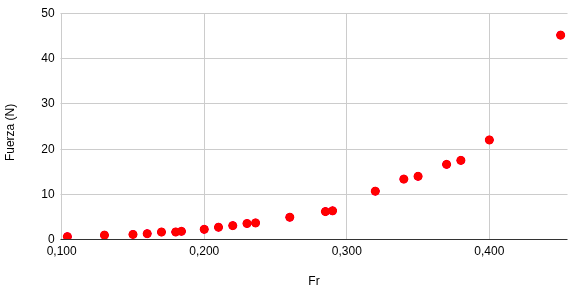
\includegraphics[width=\textwidth]{images/efd-165}
         \caption{Calado 1.}
         \label{fig:resis_tpa_165}
     \end{subfigure}
     \hfill
     \begin{subfigure}[b]{0.45\textwidth}
         \centering
         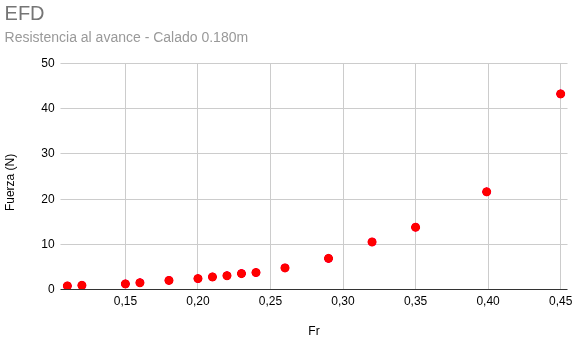
\includegraphics[width=\textwidth]{images/efd-180}
         \caption{Calado 2.}
         \label{fig:resis_tpa_180}
     \end{subfigure}
     
     \vspace{0.5cm} % Espacio entre filas
     
     % --- Segunda fila: Calado 3 centrado ---
     \begin{subfigure}[b]{0.45\textwidth}
         \centering
         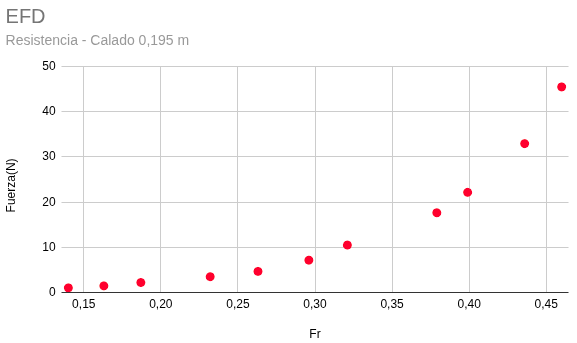
\includegraphics[width=\textwidth]{images/efd-195}
         \caption{Calado 3.}
         \label{fig:resis_tpa_195}
     \end{subfigure}
     
     \caption{Resistencia al avance (EFD) en función de Fr para diferentes calados.}
     \label{fig:comparativa_efd_calados}
\end{figure}


\subsection{Determinación experimental del factor de forma}\label{sec:det_exp_fac_form}

A partir de los resultados experimentales obtenidos para las distintas velocidades y condiciones de calado, se construyeron los diagramas del método de Prohaska, graficando $\frac{C_T}{C_F}$ frente a $\frac{Fr^4}{C_F}$ (Figura~\ref{fig:prohaska_tpa}).  
Cada conjunto de puntos corresponde a un calado diferente del \textit{P1}.  
Según el planteo teórico de \citet{prohaska1966}, los puntos deberían alinearse aproximadamente sobre una recta, cuya extrapolación al origen permite obtener el valor de $(1+k)$.  
Sin embargo, en los tres calados se observa una ligera curvatura en los puntos experimentales, especialmente a bajos números de Froude, lo que indica una desviación del comportamiento lineal esperado.

\begin{figure}[htpb]
\centering
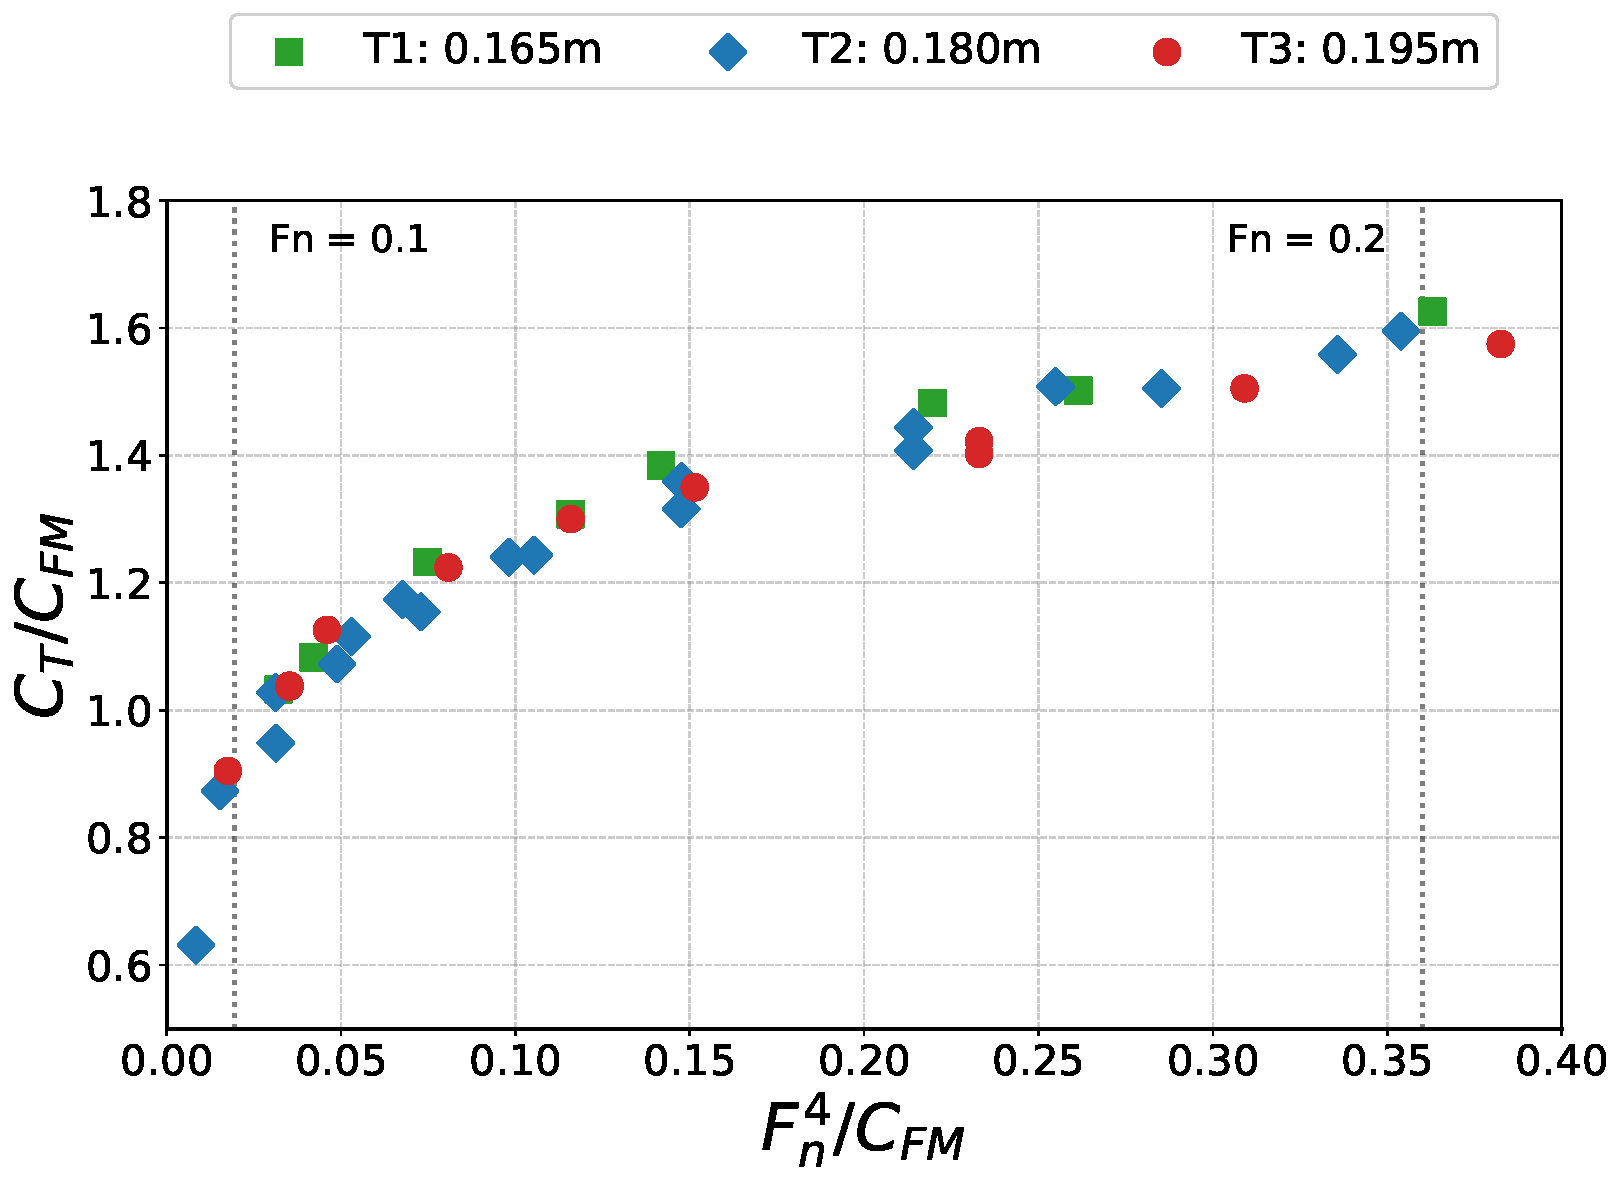
\includegraphics[width=0.6\textwidth]{images/prohaska_tpa_comparacion.pdf}
\caption{Diagramas del método de Prohaska para los tres calados del \textit{P1}. La desviación respecto de la linealidad teórica se acentúa a bajos números de Froude.}
\label{fig:prohaska_tpa}
\end{figure}

Una primera explicación de esta curvatura se relaciona con fenómenos de 
\textit{laminarización} parcial del flujo a bajas velocidades, como se describe 
en \cite{keh-sik-min}. En dichos regímenes, el flujo cercano a la proa puede 
volverse transicional o parcialmente laminar, reduciendo el coeficiente de 
fricción y alterando la pendiente esperada de la curva de Prohaska. A ello se 
suma la elevada sensibilidad del método frente a pequeñas incertidumbres en la 
medición de resistencia total, particularmente cuando el valor absoluto de la 
resistencia es muy bajo. Sin embargo, la laminarización no es la única fuente 
de desviación: como se discute en detalle en la Sección~\ref{sec:prohaska_antec}, 
las causas pueden agruparse en tres categorías: efectos geométricos no lineales 
asociados a la proa bulbo, fenómenos viscosos de separación de flujo en popas 
llenas o espejo sumergido, y curvaturas de naturaleza analítica introducidas 
por la línea de correlación ITTC-1957 o por la aproximación ${\sim}Fr^4$ para 
la resistencia por olas.

Dado que el análisis aplicado al \textit{P1} mostró cierta sensibilidad a los 
puntos considerados en la regresión lineal, se evaluaron distintos rangos de 
Froude para determinar un intervalo robusto. La Figura~\ref{fig:tpa_range} 
muestra, para el Calado~3, el valor de $(1+k)$ obtenido al variar el límite 
inferior del rango de ajuste, manteniendo fijo el límite superior en 
$Fr = 0.20$. Los otros calados presentaron un comportamiento análogo. 
Al eliminar los puntos de $Fr < 0.15$, el valor de $(1+k)$ se estabiliza, 
por lo que se adoptó el rango $0.15 < Fr < 0.20$ como intervalo de aplicación 
del método. Este comportamiento es consistente con la hipótesis de que a bajos 
$Fr$ el flujo presenta mayor proporción laminar o transicional, lo que 
distorsiona la extrapolación. A partir de $Fr \approx 0.15$, la estabilización 
del resultado sugiere que ambas condiciones del método (flujo predominantemente 
turbulento y componente por olas despreciable) se satisfacen de manera más 
razonable, aunque no puede descartarse que otros factores contribuyan a la 
mejora del ajuste.

\begin{figure}[htpb]
    \centering
    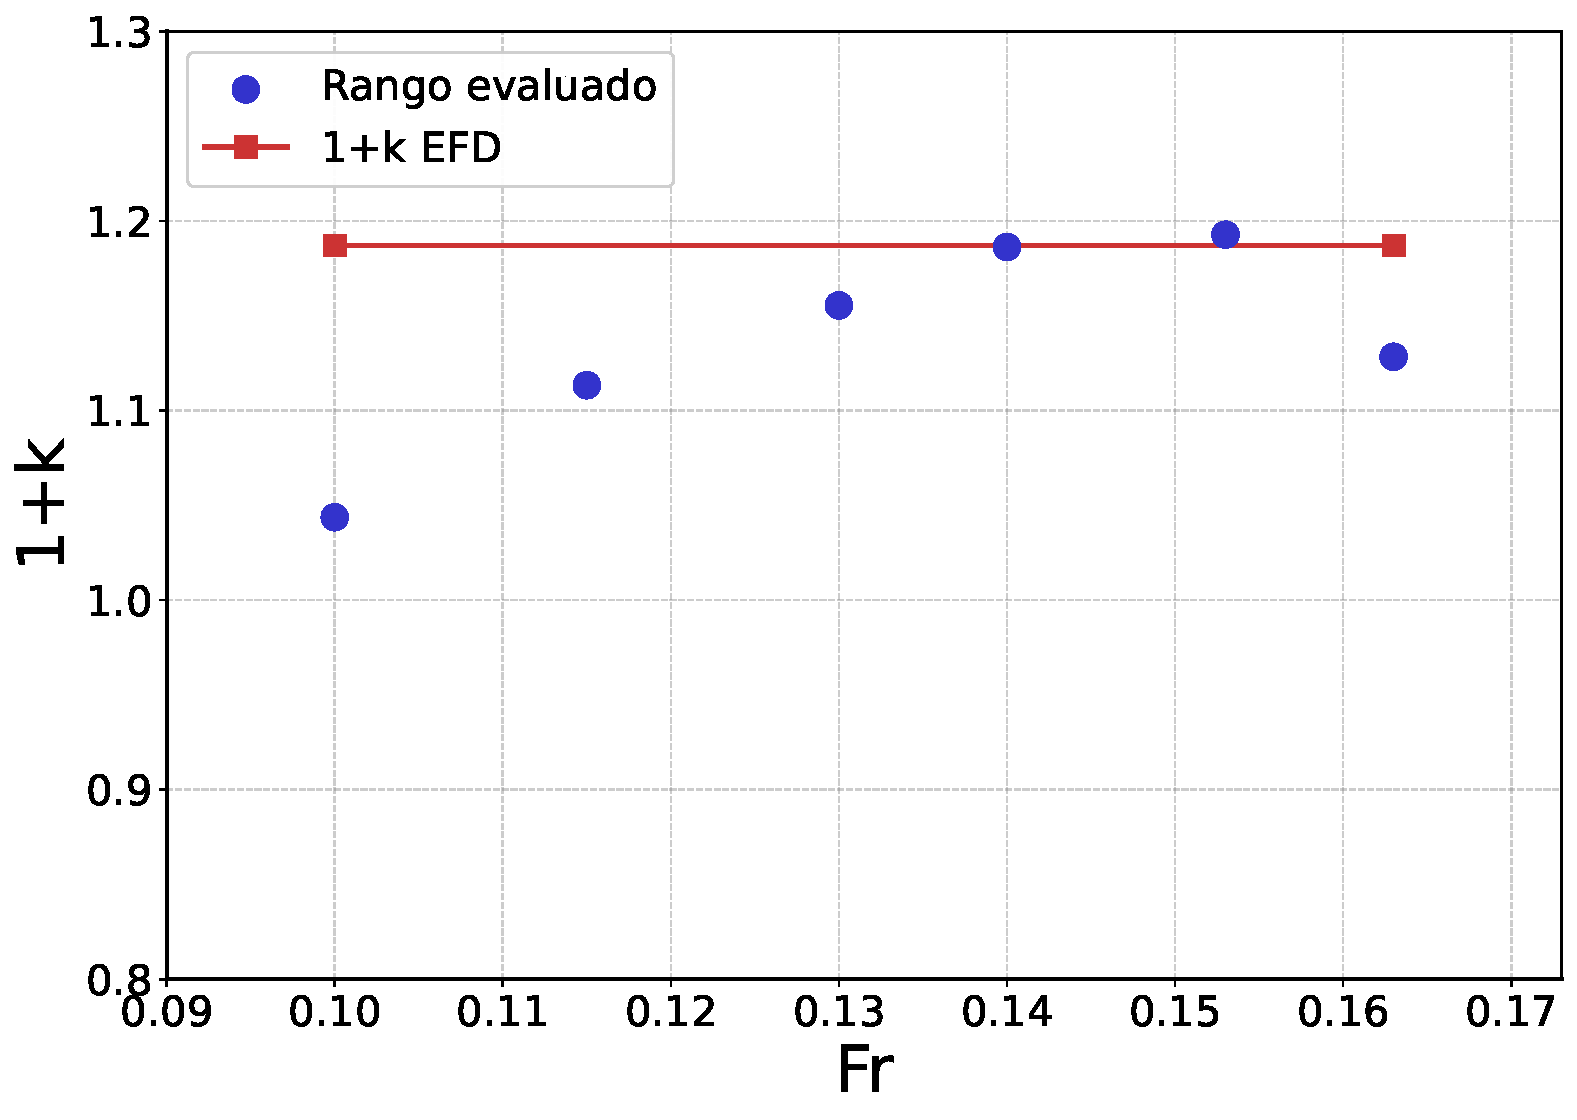
\includegraphics[width=.6\columnwidth]
        {images/efd_form_factor_tpa_range.pdf}
    \caption{Variación del factor de forma $(1+k)$ al modificar el límite 
inferior del rango de Froude (puntos azules), manteniendo el superior 
en $Fr = 0.20$. La línea roja indica el valor de $(1+k)$ adoptado 
mediante el método de Prohaska en el rango $0.15 < Fr < 0.20$. 
Calado~3; comportamiento análogo en otros calados.}
    \label{fig:tpa_range}
\end{figure}

En la Tabla \ref{tab:form_factors} se presenta el factor de forma calculado para cada calado analizado, reduciendo en cada caso el rango de Fr analizado.

\begin{table}[H]
\centering
\caption{Factor de forma $k$ para diferentes calados, calculado mediante el método de Prohaska.}
\begin{tabular}{lccc}
\hline
\textbf{Método} & \textbf{T1: 0.165 m} & \textbf{T2: 0.180 m} & \textbf{T3: 0.195 m} \\
\hline
EFD Prohaska ($k$) & 0.252 & 0.211 & 0.194 \\
\hline
\end{tabular}
\label{tab:form_factors}
\end{table}

Finalmente, para cuantificar la incertidumbre asociada al ajuste lineal, se aplicó el método propuesto por \cite{york}, que considera errores en ambos ejes y proporciona intervalos de confianza para $(1+k)$.  
La Figura~\ref{fig:york_tpa} ilustra un ejemplo del ajuste ponderado obtenido para el Calado 1.  

\begin{figure}[htpb]
\centering
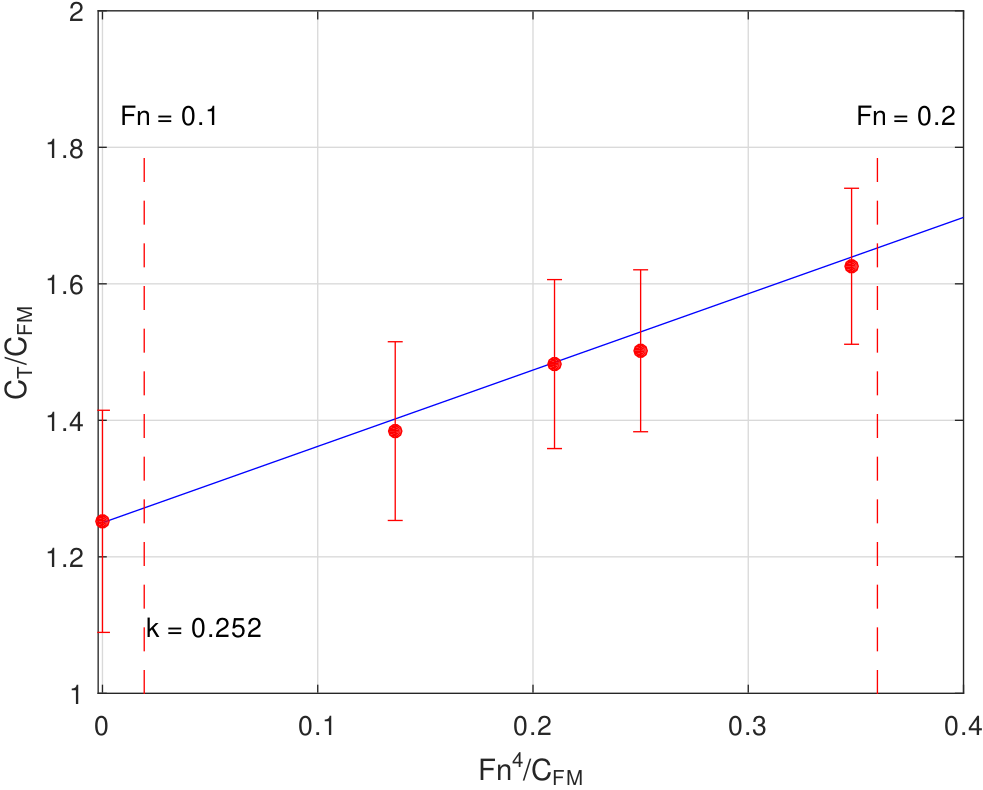
\includegraphics[width=0.6\textwidth]{images/york.png}
\caption{Ajuste lineal con ponderación mediante el método de York aplicado al \textit{P1} para la estimación de $(1+k)$ y su incertidumbre.}
\label{fig:york_tpa}
\end{figure}



En síntesis, las desviaciones observadas responden a causas de distinta 
naturaleza: algunas pueden minimizarse acotando el rango de $Fr$ analizado 
(efectos viscosos por problemas de semejanza con $Re$), otras son inherentes 
al método experimental (incertidumbre en la medición de resistencia total), 
otras son propias de las hipótesis simplificativas del método (línea de 
correlación ITTC-1957, aproximación ${\sim}Fr^4$) y otras son intrínsecas 
a la geometría del casco (proa bulbo, popa espejo sumergida). Estas últimas 
dos categorías se analizan en detalle en las 
Secciones~\ref{sec:proa_bulbo}, \ref{sec:popa_sumergida} 
y \ref{sec:linea_de_friccion}.

\vspace{1em}
\subsubsection{Modelo de referencia KCS}

Con el objetivo de analizar el comportamiento hidrodinámico de un casco 
de referencia y establecer una comparación directa con el \textit{P1}, 
se realizó una segunda campaña experimental utilizando el modelo KCS 
(escala 1:79). Este buque portacontenedores, ampliamente ensayado por 
laboratorios internacionales (KRISO, MARIN, SSPA, Hyundai), satisface 
adecuadamente los supuestos del método de Prohaska y es representativo 
de los cascos para los cuales fue desarrollado: flujo adherido en la 
región de popa, popa espejo sin inmersión significativa y componente de 
olas proporcional a $Fr^4$ en el rango de bajas velocidades. La 
comparación entre ambos cascos permite identificar qué fenómenos 
hidrodinámicos son propios del \textit{P1} y cuáles responden al 
comportamiento esperable para un casco de desplazamiento convencional.

El factor de forma experimental se determinó mediante el método de Prohaska, 
siguiendo el mismo procedimiento de ajuste aplicado al modelo \textit{P1}. 
La Figura~\ref{fig:prohaska_kcs} muestra el diagrama obtenido, donde se 
grafica $C_{TM}/C_{F0}$ frente a $Fr^4/C_{F0}$, siendo $C_{F0}$ el 
coeficiente de fricción de placa plana evaluado al número de Reynolds del 
modelo según la línea ITTC-57. Los puntos experimentales presentan una buena 
alineación sobre la recta de regresión en todo el rango analizado, en 
contraste con el comportamiento observado en el \textit{P1}. Este resultado 
es consistente con lo esperable para un casco como el KCS: la hipótesis de 
Hughes, que sustenta la descomposición de la resistencia viscosa, y la 
aproximación de Prohaska, que supone que la resistencia por olas varía como 
${\sim}Fr^4$, se satisfacen con mayor facilidad cuando el flujo permanece 
adherido y predominantemente turbulento. El KCS opera en un rango de Reynolds 
más elevado que el \textit{P1} ($Re \approx 3.84 \times 10^6$ vs 
$Re \approx 1.60 \times 10^6$ a velocidad de diseño), su proa bulbo opera 
suficientemente alejada de la superficie libre en el rango de $Fr$ analizado, 
y su popa espejo no presenta inmersión significativa, condiciones que en 
conjunto favorecen el cumplimiento de los supuestos del método.

\begin{figure}[htpb]
\centering
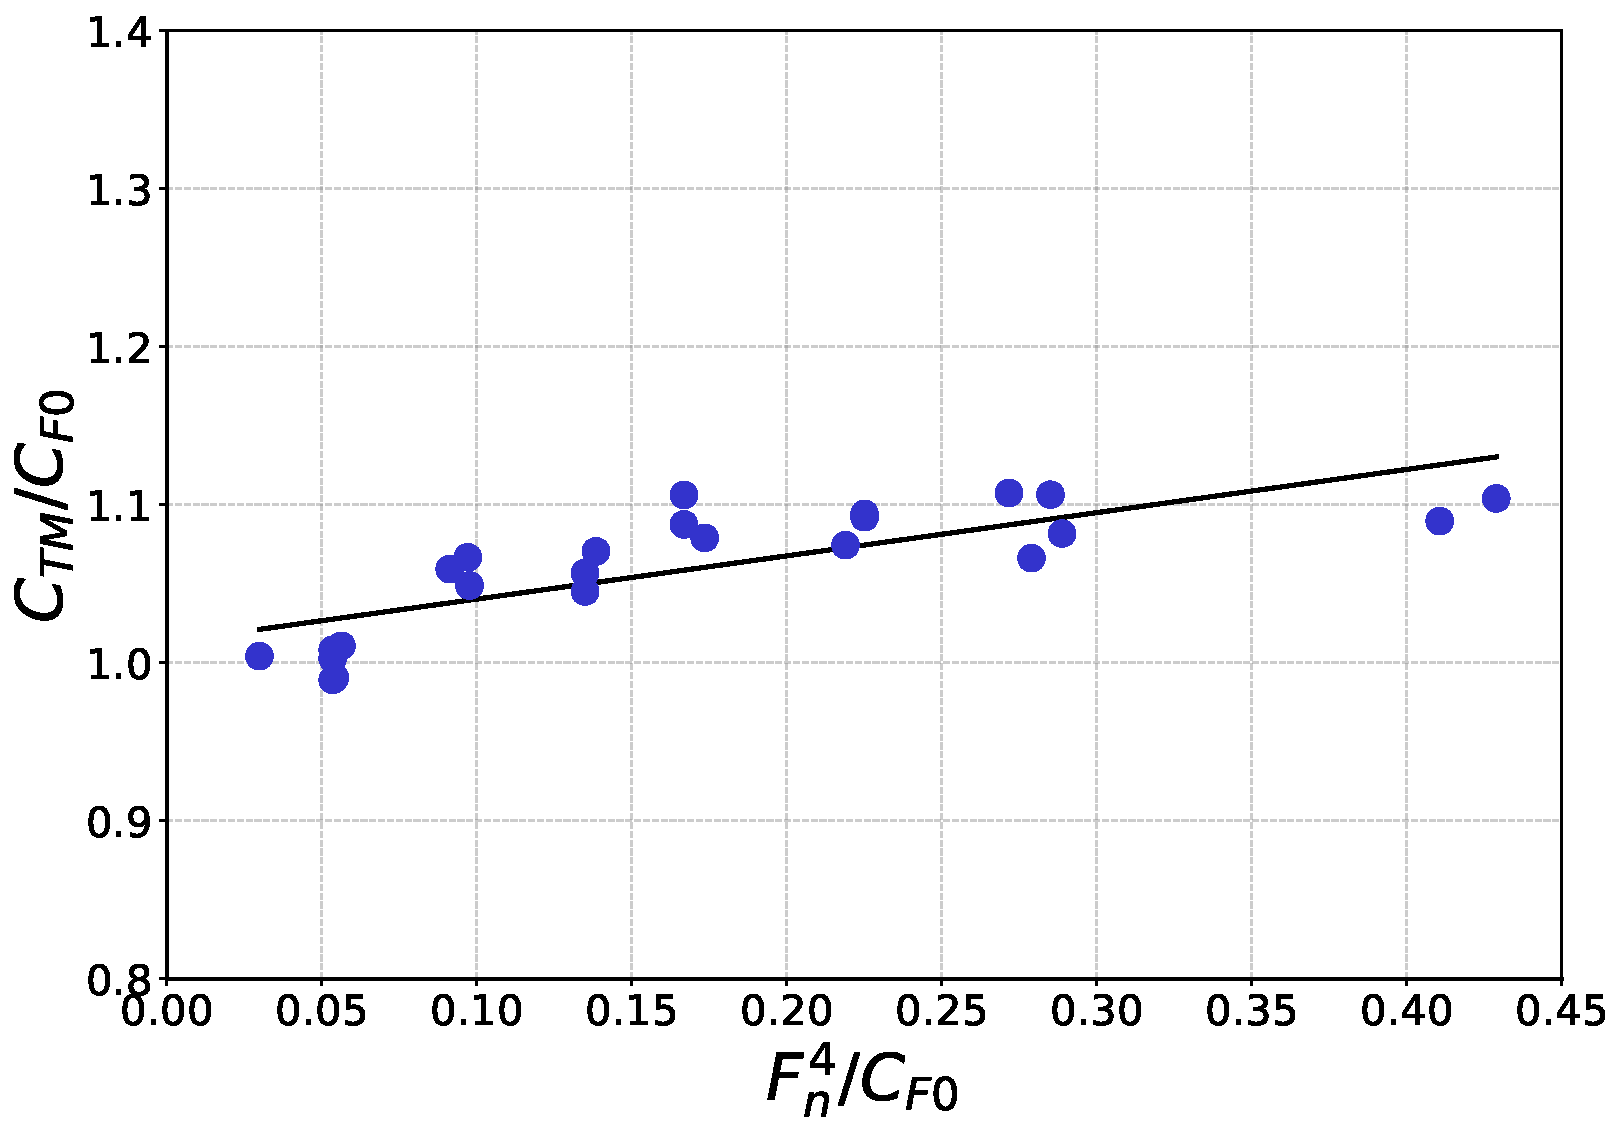
\includegraphics[width=0.6\textwidth]{images/prohaska_kcs.pdf}
\caption{Diagrama de Prohaska para el modelo KCS. Se grafica 
$C_{TM}/C_{F0}$ frente a $Fr^4/C_{F0}$, donde $C_{F0}$ es el 
coeficiente de fricción de placa plana al $Re$ del modelo según 
la línea ITTC-57. La línea continua representa el ajuste por 
mínimos cuadrados, cuya extrapolación al origen permite obtener 
el valor de $1+k$.}
\label{fig:prohaska_kcs}
\end{figure}

Posteriormente se analizó la sensibilidad del resultado al rango de velocidades 
considerado en el ajuste. La Figura~\ref{fig:kcs_range} muestra la evolución 
del valor de $(1+k)$ al variar el límite inferior del rango de $Fr$, 
manteniendo fijo el límite superior en $Fr = 0.20$. A diferencia de lo 
observado en el \textit{P1}, el valor de $(1+k)$ se estabiliza rápidamente, 
con la excepción de los puntos más bajos ($Fr < 0.11$), donde se observa 
una leve caída atribuible a posibles efectos de laminarización. El valor 
adoptado fue $(1+k) = 1.06$, correspondiente al rango $0.13 < Fr < 0.20$.

\begin{figure}[htpb]
\centering
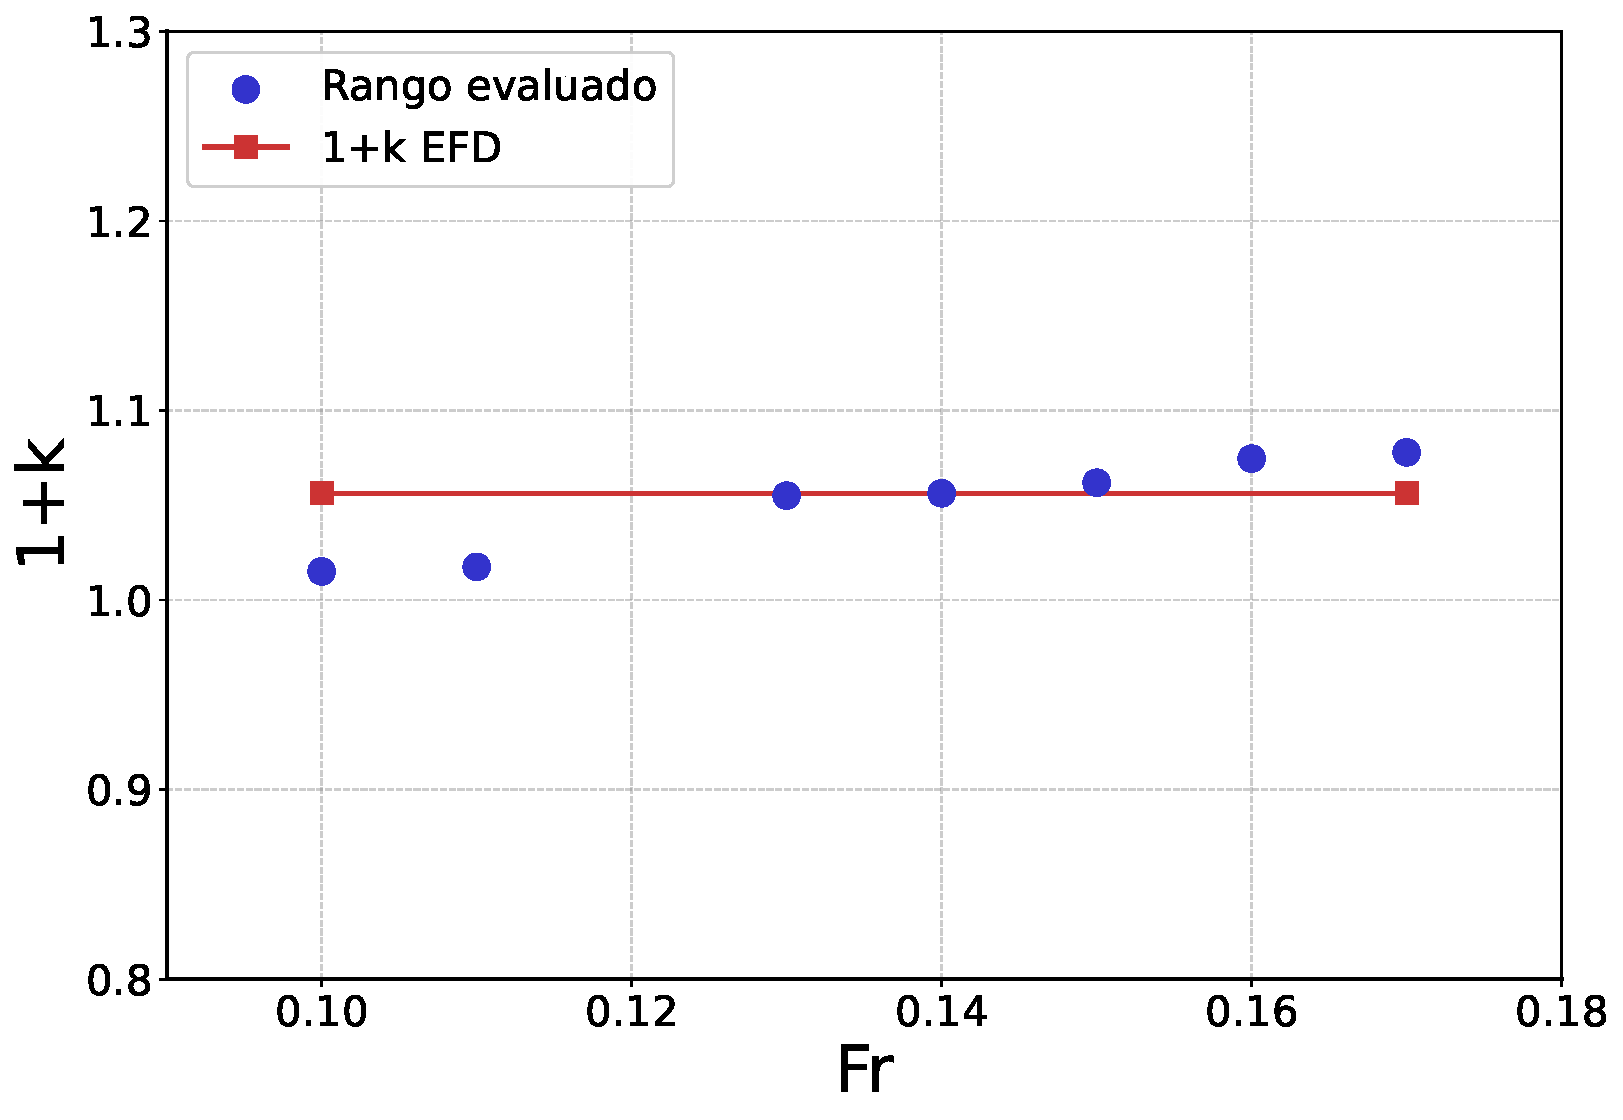
\includegraphics[width=0.6\textwidth]{images/efd_form_factor_kcs_range.pdf}
\caption{Variación del factor de forma $(1+k)$ para el modelo KCS en función 
del límite inferior del rango de Froude utilizado en el ajuste de Prohaska, 
con límite superior fijo en $Fr = 0.20$. El cuadrado rojo indica el valor 
adoptado.}
\label{fig:kcs_range}
\end{figure}

Finalmente, la Figura~\ref{fig:kcs_validation} compara el valor obtenido en 
el LabHiNO con los recopilados por \citet{TerzievDataSet} a partir de ensayos 
de distintos laboratorios internacionales. El punto del LabHiNO se ubica en 
la zona de crecimiento de $(1+k)$ con $Re$, en perfecta concordancia con la 
tendencia general de los datos de referencia, confirmando que el canal 
reproduce correctamente el comportamiento esperado para este casco a la escala 
ensayada.

\begin{figure}[htpb]
\centering
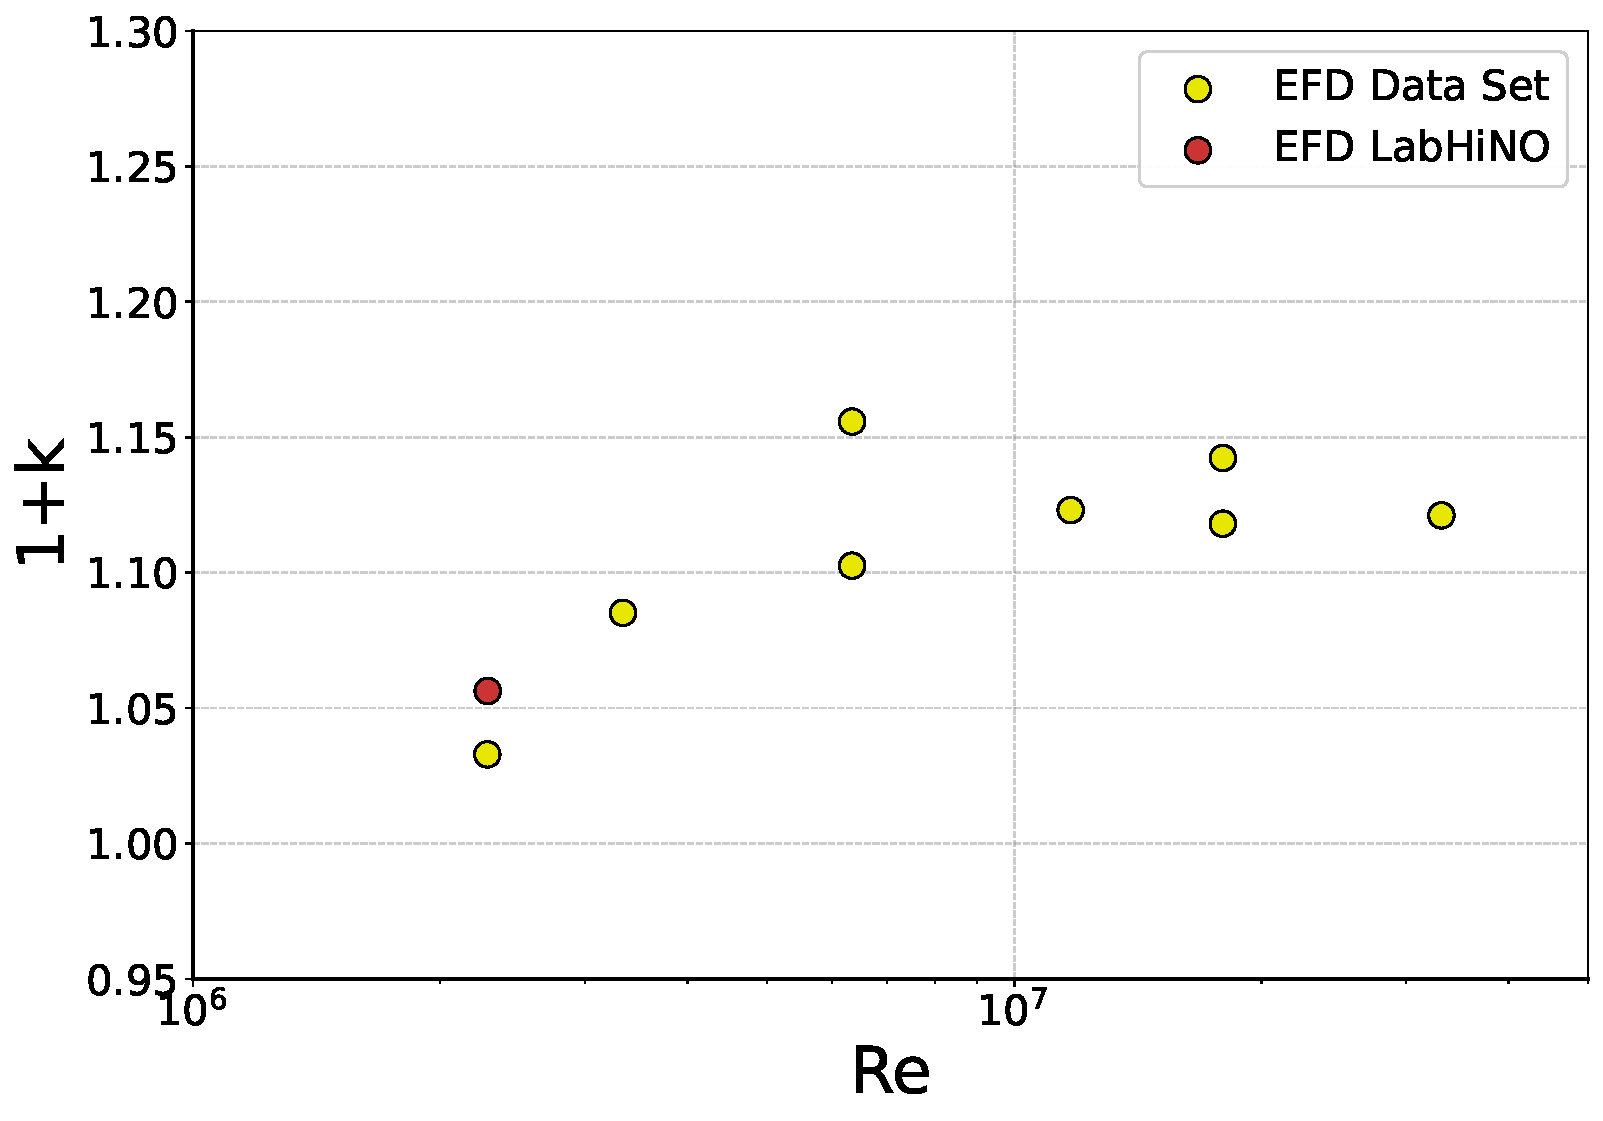
\includegraphics[width=0.6\textwidth]{images/efd_kcs_lit.pdf}
\caption{Comparación del factor de forma $(1+k)$ del KCS obtenido en el 
LabHiNO (punto rojo) con resultados experimentales históricos del KCS 
compilados de literatura internacional por \citet{TerzievDataSet} 
(puntos amarillos), en función del número de Reynolds.}
\label{fig:kcs_validation}
\end{figure}


\subsection{Ensayos computacionales de resistencia al avance}

Con el objetivo de validar la herramienta numérica y descomponer la resistencia 
total en sus componentes físicas, se replicaron computacionalmente los ensayos 
de canal descritos en la sección anterior. Las simulaciones se realizaron 
siguiendo la configuración metodológica detallada en el Capítulo~\ref{chap:Metodologia}, 
utilizando el solucionador multifásico \texttt{interFoam} para capturar la 
deformación de la superficie libre.

El dominio computacional, Figura~\ref{fig:dominio_metodologia}, reproduce las condiciones de aguas 
profundas del canal, asegurando también que las reflexiones de olas en los 
límites laterales no interfieran con la medición de resistencia en el casco. 
Las condiciones de contorno empleadas corresponden al esquema estándar 
presentado en la Tabla~\ref{tab:bc_setup}, garantizando la conservación de 
masa y la correcta generación de turbulencia en la capa límite mediante el 
modelo $k$-$\omega$ SST.

A diferencia del ensayo experimental, donde solo se obtiene la fuerza integral 
$R_{TM}$, el enfoque numérico permite separar las contribuciones de las fuerzas 
de presión y de fricción. Esta descomposición es fundamental para analizar la 
influencia de la forma del casco en la resistencia viscosa, aspecto que se 
discute en las secciones siguientes.

La validación del modelo numérico frente a los ensayos experimentales constituye 
un paso previo indispensable antes de proceder al análisis mediante el método de 
doble cuerpo. A diferencia de las simulaciones bifásicas con superficie libre, 
cuyas predicciones de resistencia total pueden cotejarse directamente con los 
resultados EFD, las simulaciones de doble cuerpo no tienen una contrapartida 
experimental directa: al eliminar la superficie libre se suprime también la 
componente de resistencia por olas, lo que imposibilita una comparación global 
con el ensayo de canal. Por este motivo, la confianza en los resultados del 
doble cuerpo descansa en la validación previa del modelo numérico completo. 
La concordancia entre EFD y CFD bifásico presentada en las 
Figuras~\ref{fig:resis_tpa_efd_cfd_165} a~\ref{fig:resis_tpa_efd_cfd_195} 
confirma que la configuración numérica, dominio, malla, modelo de turbulencia 
y condiciones de contorno, reproduce correctamente la física del problema, 
lo que respalda la confiabilidad de las simulaciones de doble cuerpo 
presentadas en la sección siguiente.

En la Figura~\ref{fig:3D-comparacion} se presenta una comparación del patrón 
de olas sobre el casco del \textit{P1} obtenido con el modelo CFD y el ensayo 
experimental (EFD), para el Calado~3 a tres números de Froude distintos 
($Fr = 0.26$, $0.37$ y $0.45$). Los tres casos ilustran la capacidad del 
modelo numérico para reproducir el patrón de olas generado por el buque en 
diferentes condiciones de velocidad.

\begin{figure}[H]
    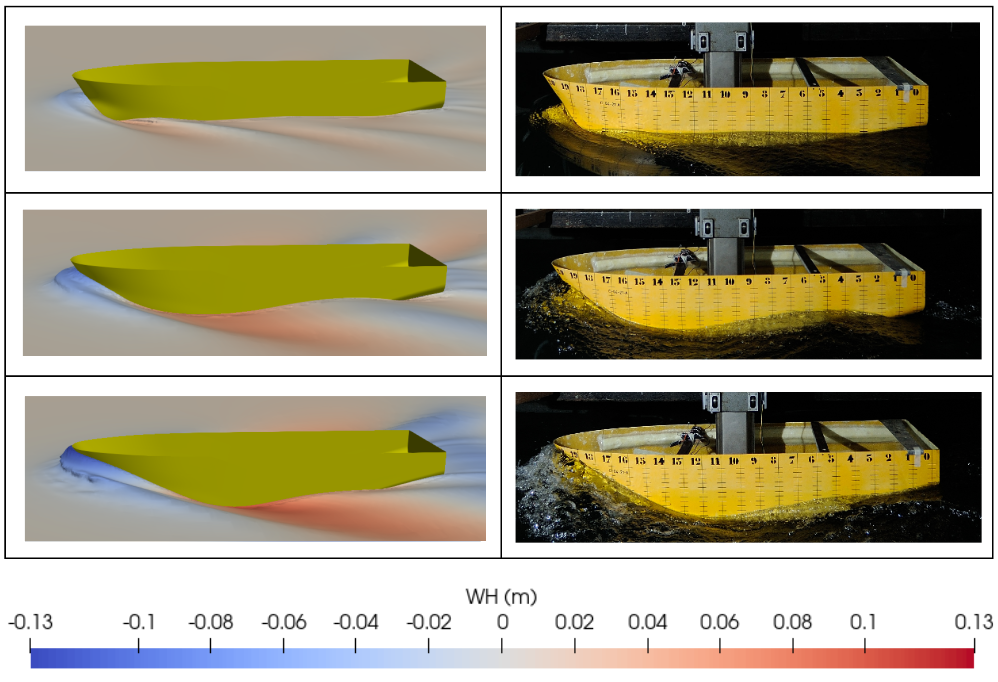
\includegraphics[width=1\linewidth]{images/3D-comparacion1.png}
    \caption{Patrón de olas sobre el \textit{P1} para distintos $Fr$ y 
    Calado~3. \textbf{Columna izquierda}: modelo CFD. 
    \textbf{Columna derecha}: EFD. 
    \textbf{Primera fila}: $Fr = 0.26$; \textbf{segunda fila}: $Fr = 0.37$; 
    \textbf{tercera fila}: $Fr = 0.45$.}
    \label{fig:3D-comparacion}
\end{figure}

En las Figuras~\ref{fig:cfd_165_tpa} a~\ref{fig:cfd_195_tpa} se presentan 
las curvas de resistencia total obtenidas para los tres calados del 
\textit{P1}. En todos los casos se observa un incremento continuo de la 
resistencia con el número de Froude, mostrando la transición habitual entre 
el régimen de bajas velocidades, donde la contribución viscosa domina el 
comportamiento global, y el rango a partir de $Fr \approx 0.30$, donde la 
componente asociada a la generación de olas comienza a desarrollarse con mayor 
intensidad. La evolución suave de las curvas y la ausencia de oscilaciones 
significativas indican que las simulaciones convergen de forma estable hacia 
un régimen estacionario, reproduciendo adecuadamente el comportamiento 
esperado para un ensayo de remolque.

\begin{figure}[htpb]
     \centering
     \begin{subfigure}[b]{0.45\textwidth}
         \centering
         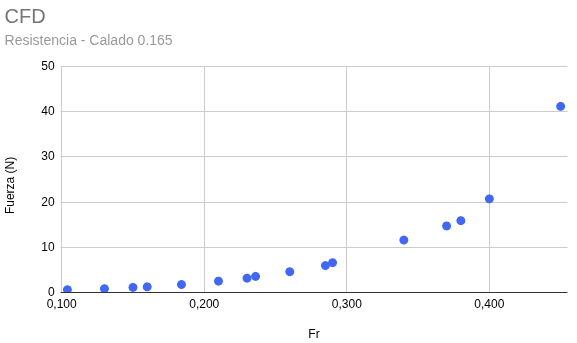
\includegraphics[width=\textwidth]{images/cfd-165}
         \caption{Calado 1.}
         \label{fig:cfd_165_tpa}
     \end{subfigure}
     \hfill
     \begin{subfigure}[b]{0.45\textwidth}
         \centering
         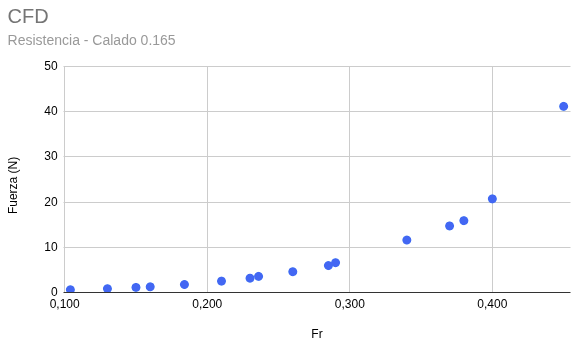
\includegraphics[width=\textwidth]{images/cfd-180}
         \caption{Calado 2.}
         \label{fig:cfd_180_tpa}
     \end{subfigure}
     
     \vspace{0.5cm}
     
     \begin{subfigure}[b]{0.45\textwidth}
         \centering
         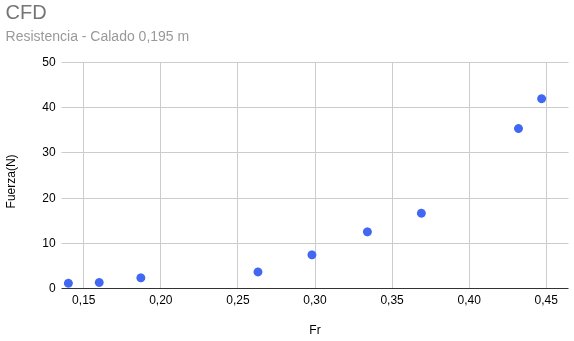
\includegraphics[width=\textwidth]{images/cfd-195}
         \caption{Calado 3.}
         \label{fig:cfd_195_tpa}
     \end{subfigure}
     
     \caption{Resistencia al avance del \textit{P1} obtenida por CFD en 
     función de $Fr$ para los tres calados.}
     \label{fig:comparativa_calados}
\end{figure}


\subsection{Determinación numérica del factor de forma}\label{sec:det_num_fac_form}

Para la determinación computacional del factor de forma se implementaron dos métodos. El primero fue repetir lo propuesto por Prohaska para lo tres calados con el dominio presentado en la Figura \ref{fig:dominio_metodologia}, mientras que el segundo, que será tratado en detalle en la Sección \ref{sec:4.1.5_enfoque_doble_cuerpo}, implica la simulación únicamente de la obra viva eliminando la superficie libre. El primer método permite una comparación directa con el ensayo experimental. Como sucedió en los ensayos experimentales, a bajas velocidades también se observa en los ensayos CFD una separación de los puntos respecto de la recta teórica esperada, pero esta vez de forma cóncava en lugar de convexa, como se ve en la Figura \ref{fig:prohaska_tpa_cfd}.


\begin{figure}[htpb]
\centering
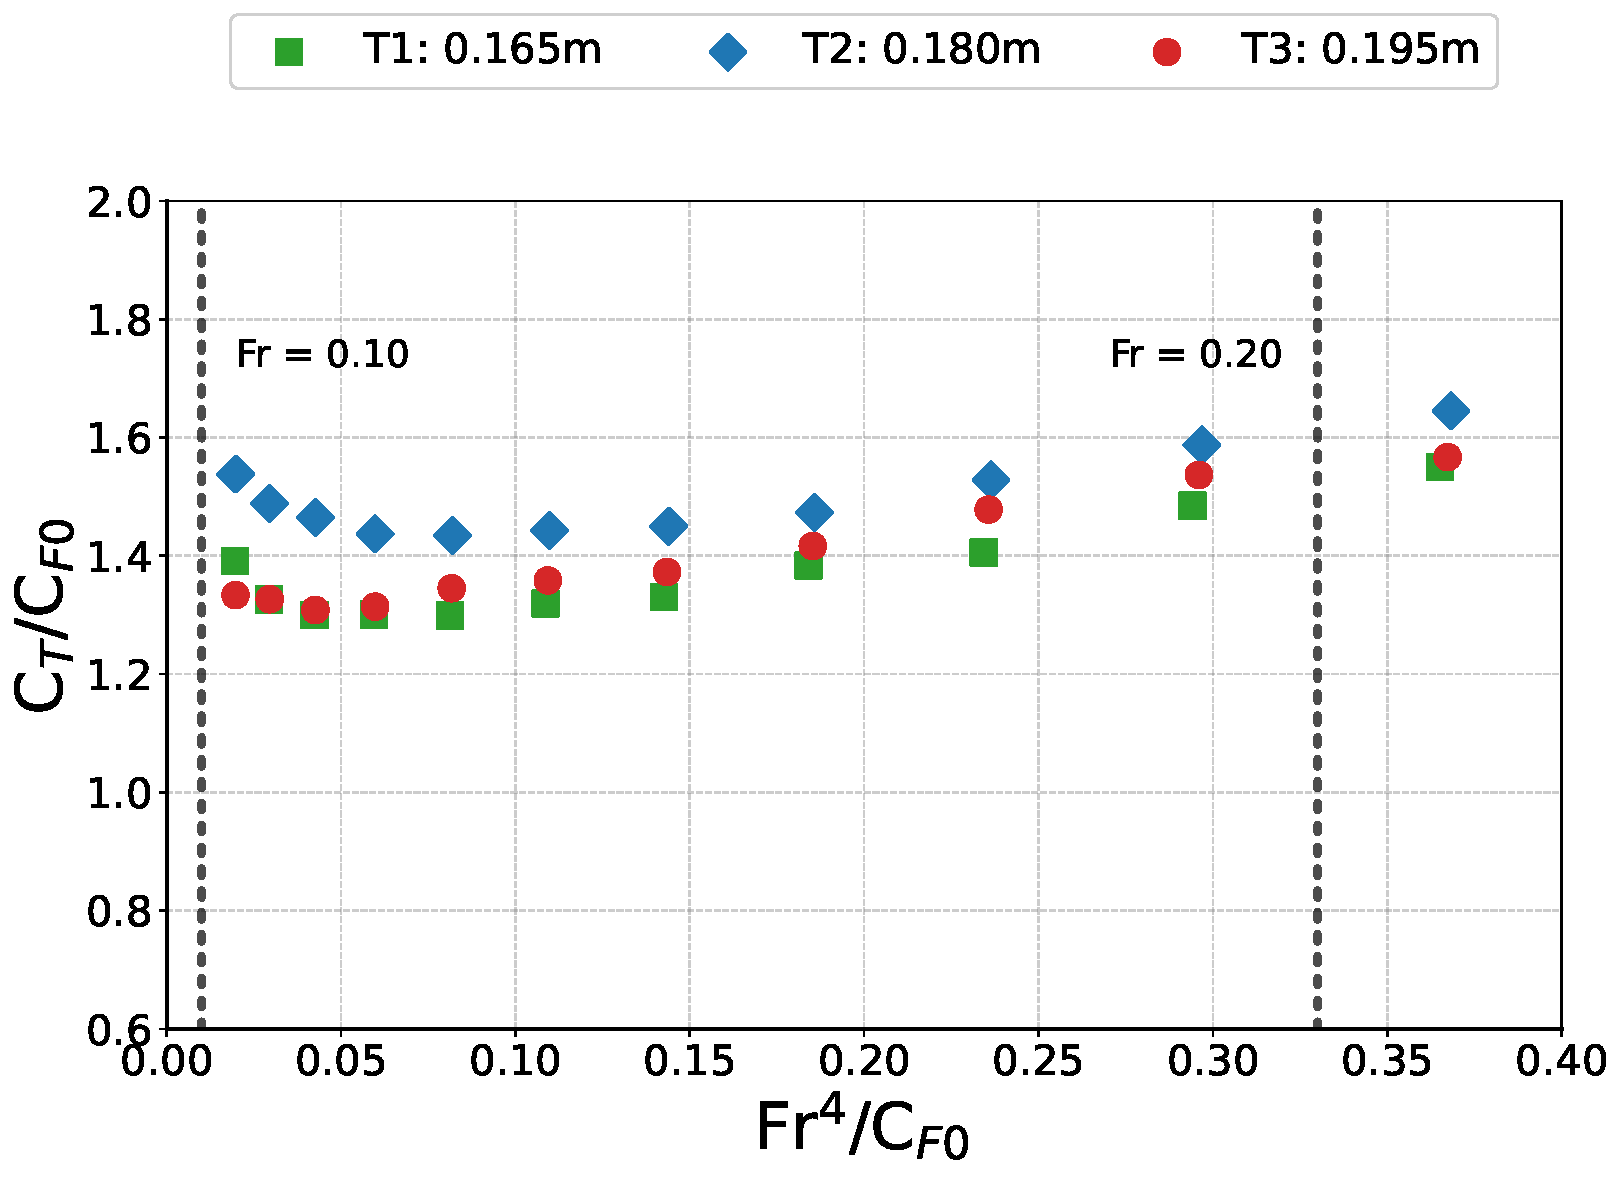
\includegraphics[width=0.6\textwidth]{images/prohaska_tpa_cfd_comparacion.pdf}
\caption{Diagramas del método de Prohaska para los tres calados del \textit{P1}. La desviación respecto de la linealidad teórica se acentúa a bajos números de Froude.}
\label{fig:prohaska_tpa_cfd}
\end{figure}

La diferencia observada a bajas velocidades sugiere una deficiencia en el modelado de la zona de transición. Dado que el modelo $k-\omega$ SST asume un régimen turbulento, carece de la sensibilidad necesaria para capturar correctamente la transición de la capa límite en las simulaciones. El punto de transición suele verse adelantado por los modelos que asumen flujo turbulento. 

Al igual que se hizo con los ensayos experimentales, se repite el análisis de rangos de Froude para el análisis computacional del factor de forma. Dado que los tres calados presentaron un comportamiento análogo, tanto en la 
forma de la curva como en la sensibilidad al rango de Froude considerado, 
presentar los resultados de cada uno por separado no aportaría información 
adicional sino que recargaría innecesariamente la exposición. Por este motivo, 
de aquí en adelante el análisis se centra en el Calado~3, que corresponde a la 
condición de plena carga y resulta el más representativo del régimen de operación del \textit{P1}. La Figura~\ref{fig:tpa_range_cfd} muestra la variación de $(1+k)$ en función del límite inferior del rango de Froude utilizado en el ajuste de Prohaska, con límite superior fijo en $Fr = 0.20$, junto con el valor adoptado como representativo del factor de forma para este calado.

\begin{figure}[htpb]
	\centering
	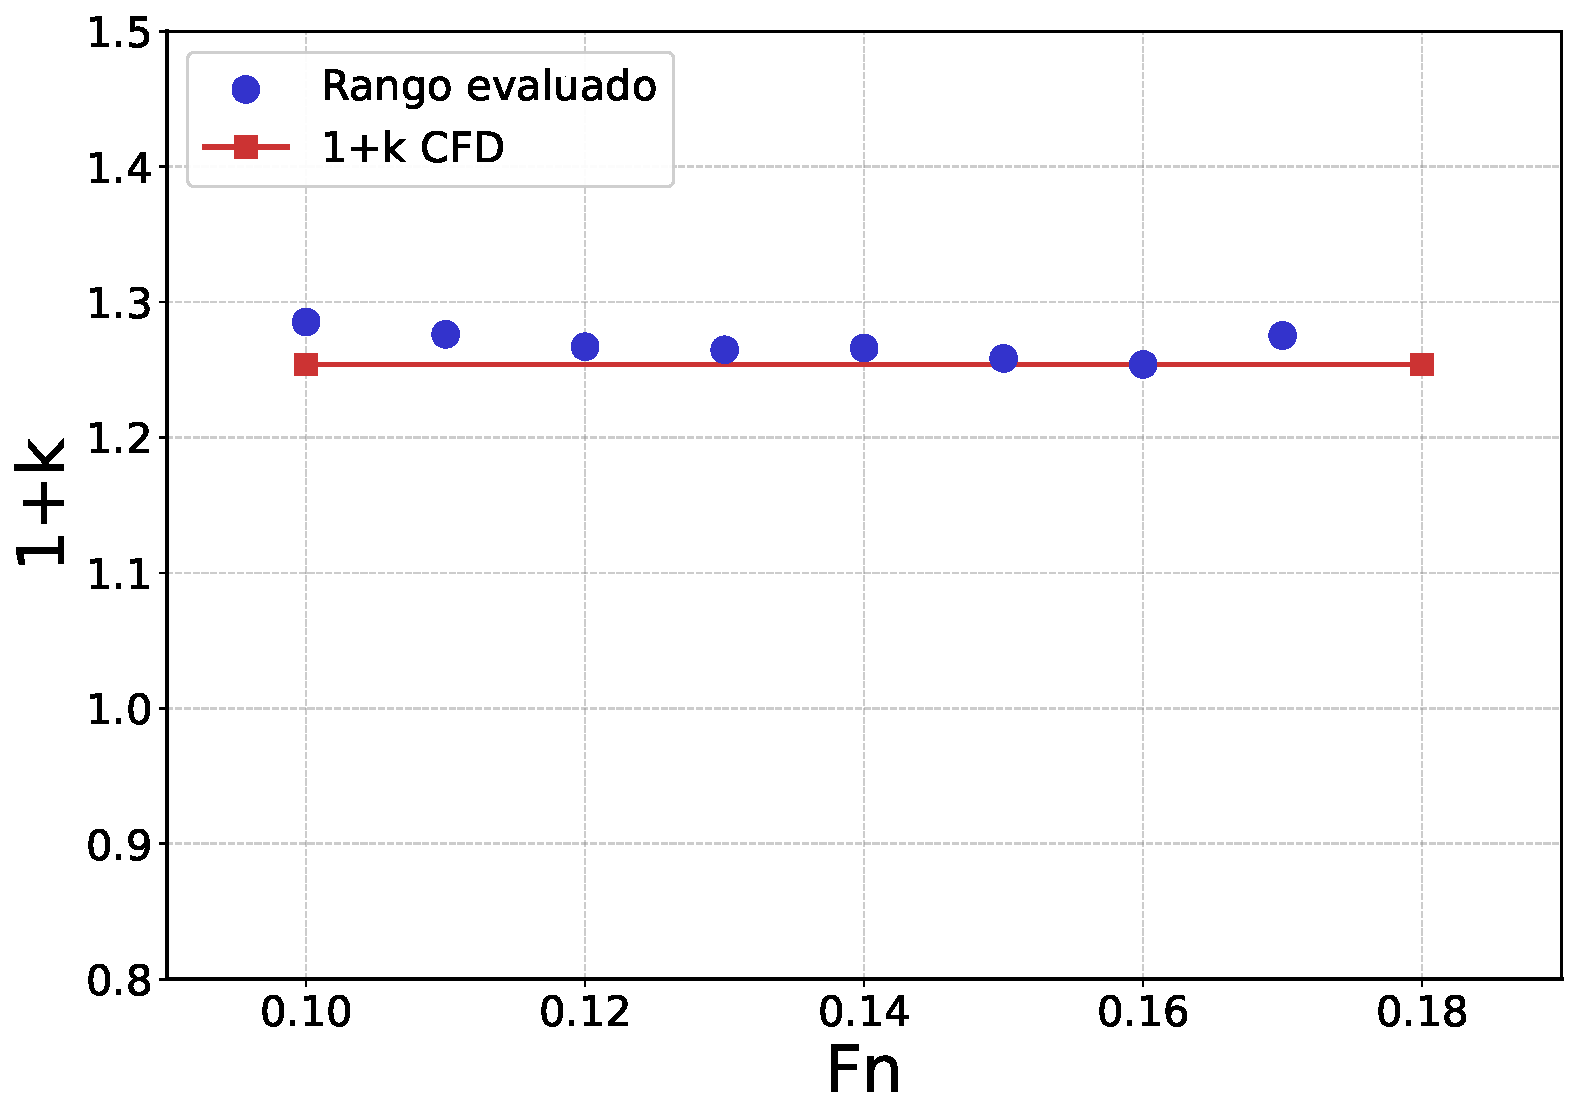
\includegraphics[width=.6\columnwidth]{images/cfd_form_factor_tpa_195_range.pdf}
	\caption{Variación del factor de forma experimental $(1+k)$ para el \textit{P1} en función del rango de Froude utilizado en el ajuste de Prohaska. Calado 3}
\label{fig:tpa_range_cfd}
\end{figure}

\subsection{Enfoque de Doble Cuerpo}\label{sec:4.1.5_enfoque_doble_cuerpo}

Ante las dificultades observadas para aplicar el método de Prohaska en el 
entorno numérico, debido a la incertidumbre en la transición de la turbulencia 
y la curvatura observada en el diagrama $C_{TM}/C_{F0}$ vs $Fr^4/C_{F0}$ a 
bajas velocidades, se optó por una estrategia alternativa: el método de 
\textit{doble cuerpo}, descripto en la Sección~\ref{sec:doble_cuerpo}.

Como se detalló en la Sección \ref{sec:doble_cuerpo}, este enfoque elimina la superficie libre y la formación de olas, modelando el fluido como un medio infinito y el casco como un cuerpo reflejado (ver Figura \ref{fig:double_body_domain}). Esto permite aislar la resistencia viscosa ($R_V$) y calcular el factor de forma $(1+k)$ directamente para cada velocidad mediante la relación $C_V / C_{F0}$, sin depender de la extrapolación a velocidad cero.

\subsubsection{Análisis del \textit{P1}}


Antes de interpretar el comportamiento físico del factor de forma, se
verifica la fiabilidad numérica de las simulaciones en las cuatro escalas
geométricas. La Tabla~\ref{tab:CFD_summary_compact} resume, para cada número
de Froude, el número de Reynolds, la resolución de pared ($y^+$), el factor de
forma $(1+k)$ y el índice de convergencia de malla (GCI).

\begin{table}[htbp]
\centering
\caption{Resumen de las simulaciones CFD para las cuatro escalas geométricas
del \textit{P1} (Calado~3): número de Reynolds, resolución de pared ($y^+$),
factor de forma $(1+k)$ e índice de convergencia de malla (GCI) para cada
número de Froude. Modelo de turbulencia: $k$--$\omega$ SST.}
\label{tab:CFD_summary_compact}
\footnotesize
\begin{tabularx}{\textwidth}{>{\bfseries}c *{4}{>{\centering\arraybackslash}X}}
\toprule
\textbf{Fr} & \textbf{1:20} & \textbf{1:10} & \textbf{1:5} & \textbf{1:1} \\
\midrule
\multicolumn{5}{c}{\textbf{Número de Reynolds}} \\[-0.3em]
\multicolumn{5}{c}{\rule{\dimexpr\textwidth-2\tabcolsep}{0.2pt}} \\[0.4em]
\textbf{0.100} & $6.40\times10^{5}$ & $1.81\times10^{6}$ & $5.12\times10^{6}$ & $5.73\times10^{7}$ \\
\textbf{0.160} & $1.02\times10^{6}$ & $2.90\times10^{6}$ & $8.20\times10^{6}$ & $9.17\times10^{7}$ \\
\textbf{0.200} & $1.28\times10^{6}$ & $3.62\times10^{6}$ & $1.02\times10^{7}$ & $1.15\times10^{8}$ \\
\textbf{0.240} & $1.54\times10^{6}$ & $4.35\times10^{6}$ & $1.23\times10^{7}$ & $1.37\times10^{8}$ \\
\textbf{0.300} & $1.92\times10^{6}$ & $5.43\times10^{6}$ & $1.54\times10^{7}$ & $1.72\times10^{8}$ \\
\textbf{0.360} & $2.31\times10^{6}$ & $6.52\times10^{6}$ & $1.84\times10^{7}$ & $2.06\times10^{8}$ \\
\textbf{0.400} & $2.56\times10^{6}$ & $7.25\times10^{6}$ & $2.05\times10^{7}$ & $2.29\times10^{8}$ \\
\midrule
\multicolumn{5}{c}{\textbf{Resolución de pared ($y^+$)}} \\[-0.3em]
\multicolumn{5}{c}{\rule{\dimexpr\textwidth-2\tabcolsep}{0.2pt}} \\[0.4em]
\textbf{0.100} & 0.40 & 8.42$^{c}$ & 12.0 & 108 \\
\textbf{0.160} & 0.70 & 9.00 & 17.0 & 168 \\
\textbf{0.200} & 1.03 & 11.0 & 22.0 & 207 \\
\textbf{0.240} & 1.40 & 11.4 & 26.0 & 245 \\
\textbf{0.300} & 2.23 & 12.6 & 32.0 & 302 \\
\textbf{0.360} & 2.70 & 14.6 & 38.0 & 353 \\
\textbf{0.400} & 3.00 & 15.9 & 41.0 & 389 \\
\midrule
\multicolumn{5}{c}{\textbf{Factor de forma $(1+k)$}} \\[-0.3em]
\multicolumn{5}{c}{\rule{\dimexpr\textwidth-2\tabcolsep}{0.2pt}} \\[0.4em]
\textbf{0.100} & 1.179 & 1.399 & 1.489 & 1.654 \\
\textbf{0.160} & 1.251 & 1.622$^{b}$ & 1.484 & 1.690 \\
\textbf{0.200} & 1.320 & 1.570 & 1.501 & 1.713 \\
\textbf{0.240} & 1.378 & 1.513 & 1.522 & 1.714 \\
\textbf{0.300} & 1.470 & 1.465 & 1.528 & 1.727 \\
\textbf{0.360} & 1.598 & 1.465 & 1.548 & 1.731 \\
\textbf{0.400} & 1.637 & 1.473 & 1.554 & 1.745 \\
\midrule
\multicolumn{5}{c}{\textbf{Índice de convergencia de malla (GCI) [\%]}} \\[-0.3em]
\multicolumn{5}{c}{\rule{\dimexpr\textwidth-2\tabcolsep}{0.2pt}} \\[0.4em]
\textbf{0.100} & 0.028 & 0.773 & 1.748 & 0.002 \\
\textbf{0.160} & 0.112 & 1.032 & 0.005 & 0.849 \\
\textbf{0.200} & 0.009 & 3.722 & 0.859 & 3.730 \\
\textbf{0.240} & 0.003 & 2.193 & 0.723 & 3.985 \\
\textbf{0.300} & 0.002 & 0.001 & 3.544 & 1.681 \\
\textbf{0.360} & 1.382 & 0.003 & 0.311 & 2.053 \\
\textbf{0.400} & 13.433$^{a}$ & 0.011 & 0.090 & 4.421 \\
\bottomrule
\end{tabularx}

\vspace{0.4em}
{\footnotesize\raggedright
$^{a}$~El punto 1:20 / $Fr = 0{.}400$ presenta $GCI = 13{.}4\%$, atribuible a
la complejidad del campo de flujo a alta velocidad; esta condición queda fuera
del rango operativo del buque ($Fr \lesssim 0{.}36$) y no se considera en el
análisis de efectos de escala.\\
$^{b}$~El valor $1+k = 1{.}622$ en 1:10 / $Fr = 0{.}160$ ($y^+ = 9{.}0$) se
aparta de la tendencia de su columna; su ubicación en la región
\textit{buffer}, por debajo del umbral de conmutación de la función de pared,
sugiere un origen numérico asociado al tratamiento de pared más que físico.\par}
\end{table}

Dado que las cuatro escalas geométricas se simularon con mallas
geométricamente similares, la distancia media a la pared en unidades de pared
crece con el número de Reynolds: desde $y^+ \sim 1$ en la menor escala de
modelo hasta $y^+ > 300$ en escala buque. La escala 1:20 resuelve la subcapa
viscosa ($y^+ \lesssim 5$), mientras que las mallas de escala buque ubican el
primer centro de celda dentro de la capa logarítmica
($30 \lesssim y^+ \lesssim 300$), rango de operación previsto para el enfoque
de funciones de pared. Las dos escalas intermedias (1:10 y 1:5) se sitúan
mayormente en la región \textit{buffer} ($5 \lesssim y^+ \lesssim 30$). En
esta región, la formulación de $\omega$ empleada por el modelo $k$--$\omega$
SST combina de forma continua las expresiones viscosa y logarítmica
\citep{Menter1994}, lo que le confiere una relativa insensibilidad a la
posición de la primera celda; no obstante, la región \textit{buffer}
constituye el régimen de menor fiabilidad para el tratamiento de pared, por lo
que las escalas intermedias deben interpretarse con mayor cautela que las
escalas resuelta y de capa logarítmica.

Esta menor fiabilidad se refleja en la dispersión local del factor de forma:
en las escalas intermedias, los valores de $(1+k)$ varían de manera no
monótona con la velocidad y alcanzan índices de convergencia de malla de hasta
aproximadamente un 4\%, en consistencia con la mayor incertidumbre numérica de
la componente de presión viscosa reportada para las simulaciones de doble
cuerpo \citep{KORKMAZ2022112590}. Los resultados de escala buque, que son los
que sustentan las conclusiones de esta tesis, resultan en cambio suaves y
monótonos con el número de Reynolds ($1+k$ crece de $1{.}654$ a $1{.}745$ en el
rango analizado), se ubican en el rango de $y^+$ válido para las funciones de
pared y no presentan cambios de pendiente ni anomalías. La tendencia de
$(1+k)$ a crecer con $Re$ sin alcanzar un valor asintótico es, por lo tanto,
robusta: se sostiene tanto en la escala buque, resuelta en un régimen de pared
adecuado, como en la consistencia global de la curva, aun cuando algunos
puntos individuales de la región \textit{buffer} se dispersen en torno a ella.

La Figura \ref{fig:tpa_DB_k_evolucion} muestra la distribución del factor de forma calculado para los tres calados analizados empleando la configuración de malla verificada en la Sección~\ref{sec:convergencia_de_malla}. Contrario a la hipótesis clásica de la ITTC, que asume un factor de forma constante e independiente de la velocidad ($k \neq f(Fr, Re)$), los resultados obtenidos revelan una variación significativa y sistemática de $(1+k)$ a lo largo del rango de Froude evaluado.

Este hallazgo resulta crítico: si el factor de forma varía de manera apreciable dentro de la misma escala, la selección de un valor único para el proceso de extrapolación a escala buque se vuelve inherentemente ambigua. Más aún, la tendencia creciente observada sugiere una fuerte dependencia con el número de Reynolds, una problemática de efectos de escala que se abordará en profundidad en la Sección \ref{sec:analisis_efectos_escala}.

\begin{figure}[htpb]
    \centering
    % Primera fila: Calado 1 y Calado 2
    \begin{subfigure}[b]{0.48\textwidth}
        \centering
        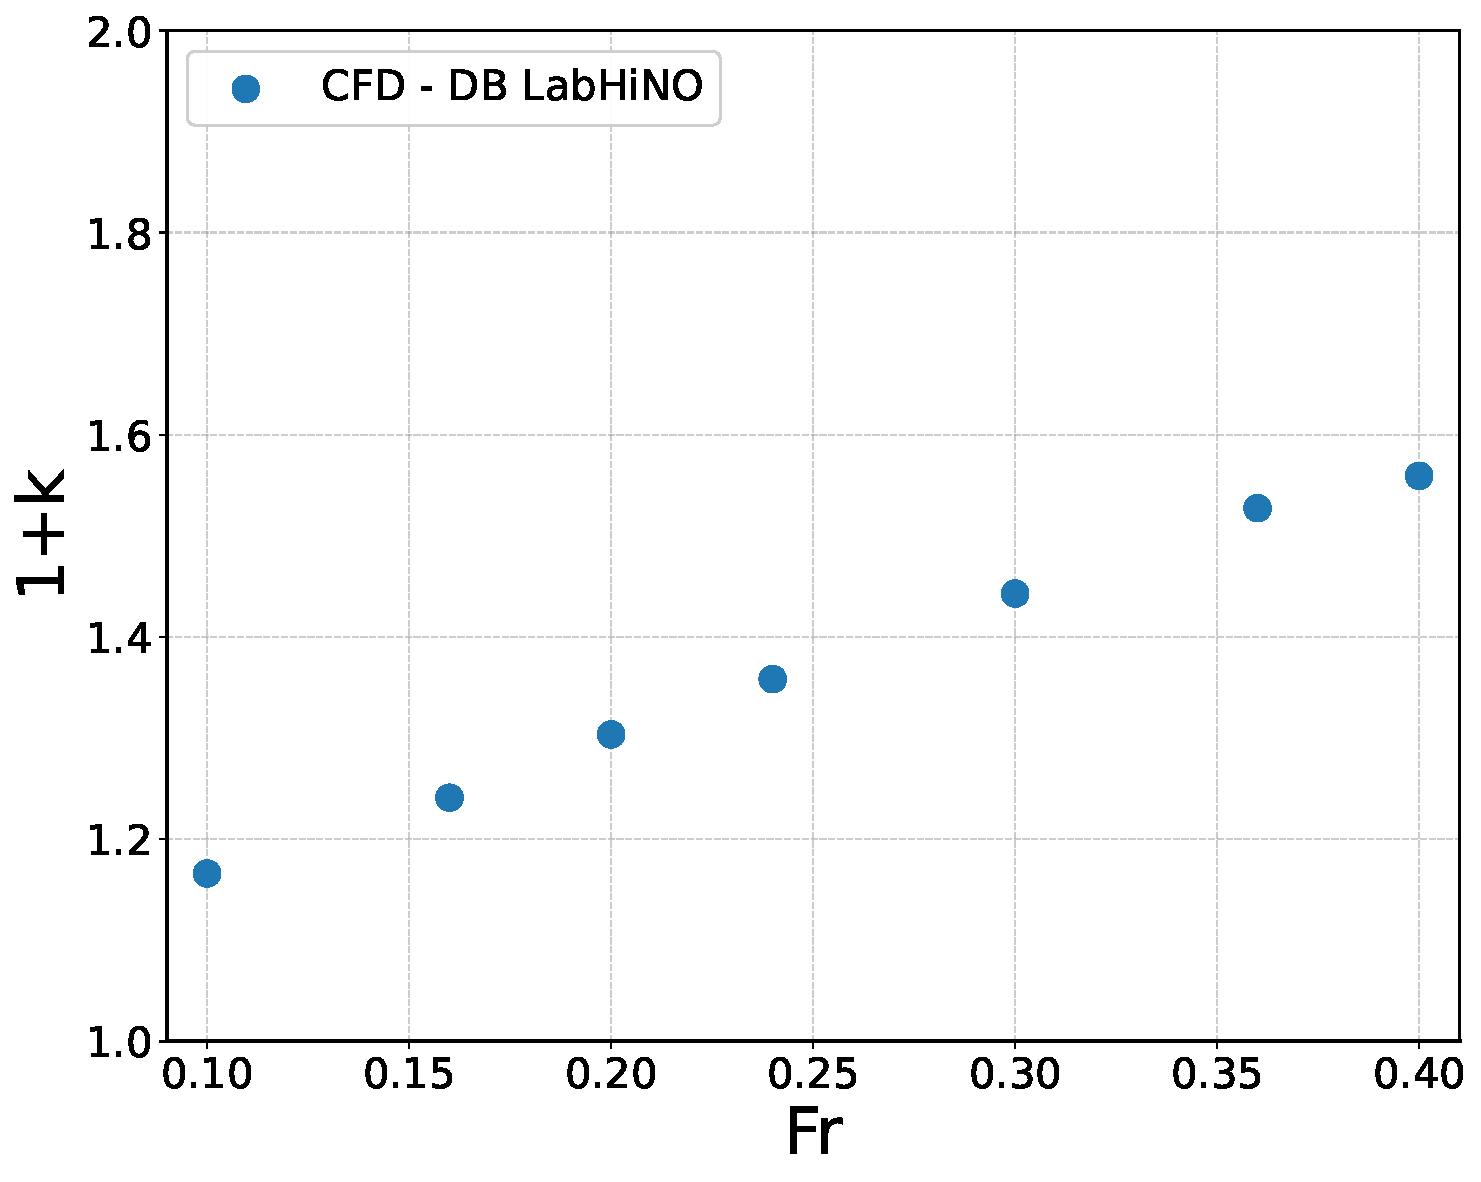
\includegraphics[width=\textwidth]{images/tpa_CFD_DB_165.pdf}
        \caption{Calado 1 (T1: 0.165 m)}
        \label{fig:k_165}
    \end{subfigure}
    \hfill
    \begin{subfigure}[b]{0.48\textwidth}
        \centering
        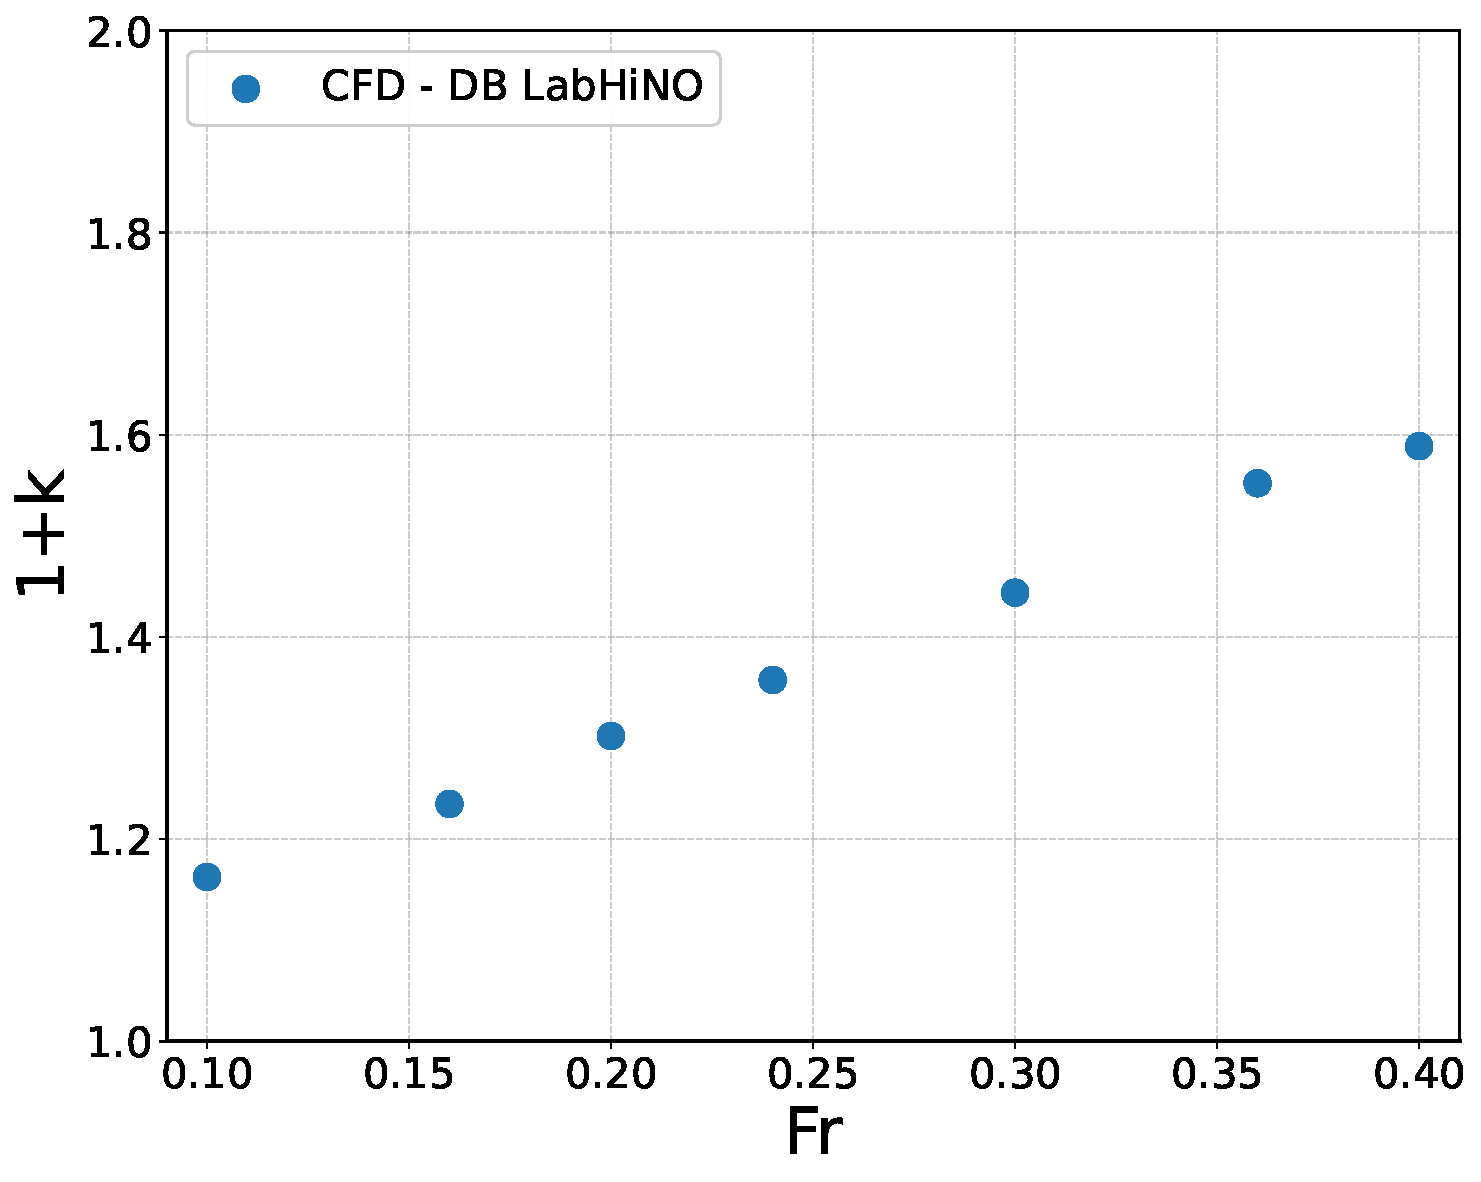
\includegraphics[width=\textwidth]{images/tpa_CFD_DB_180.pdf}
        \caption{Calado 2 (T2: 0.180 m)}
        \label{fig:k_180}
    \end{subfigure}
    
    \vspace{10pt} % Espacio entre filas
    
    % Segunda fila: Calado 3 centrado
    \begin{subfigure}[b]{0.48\textwidth}
        \centering
        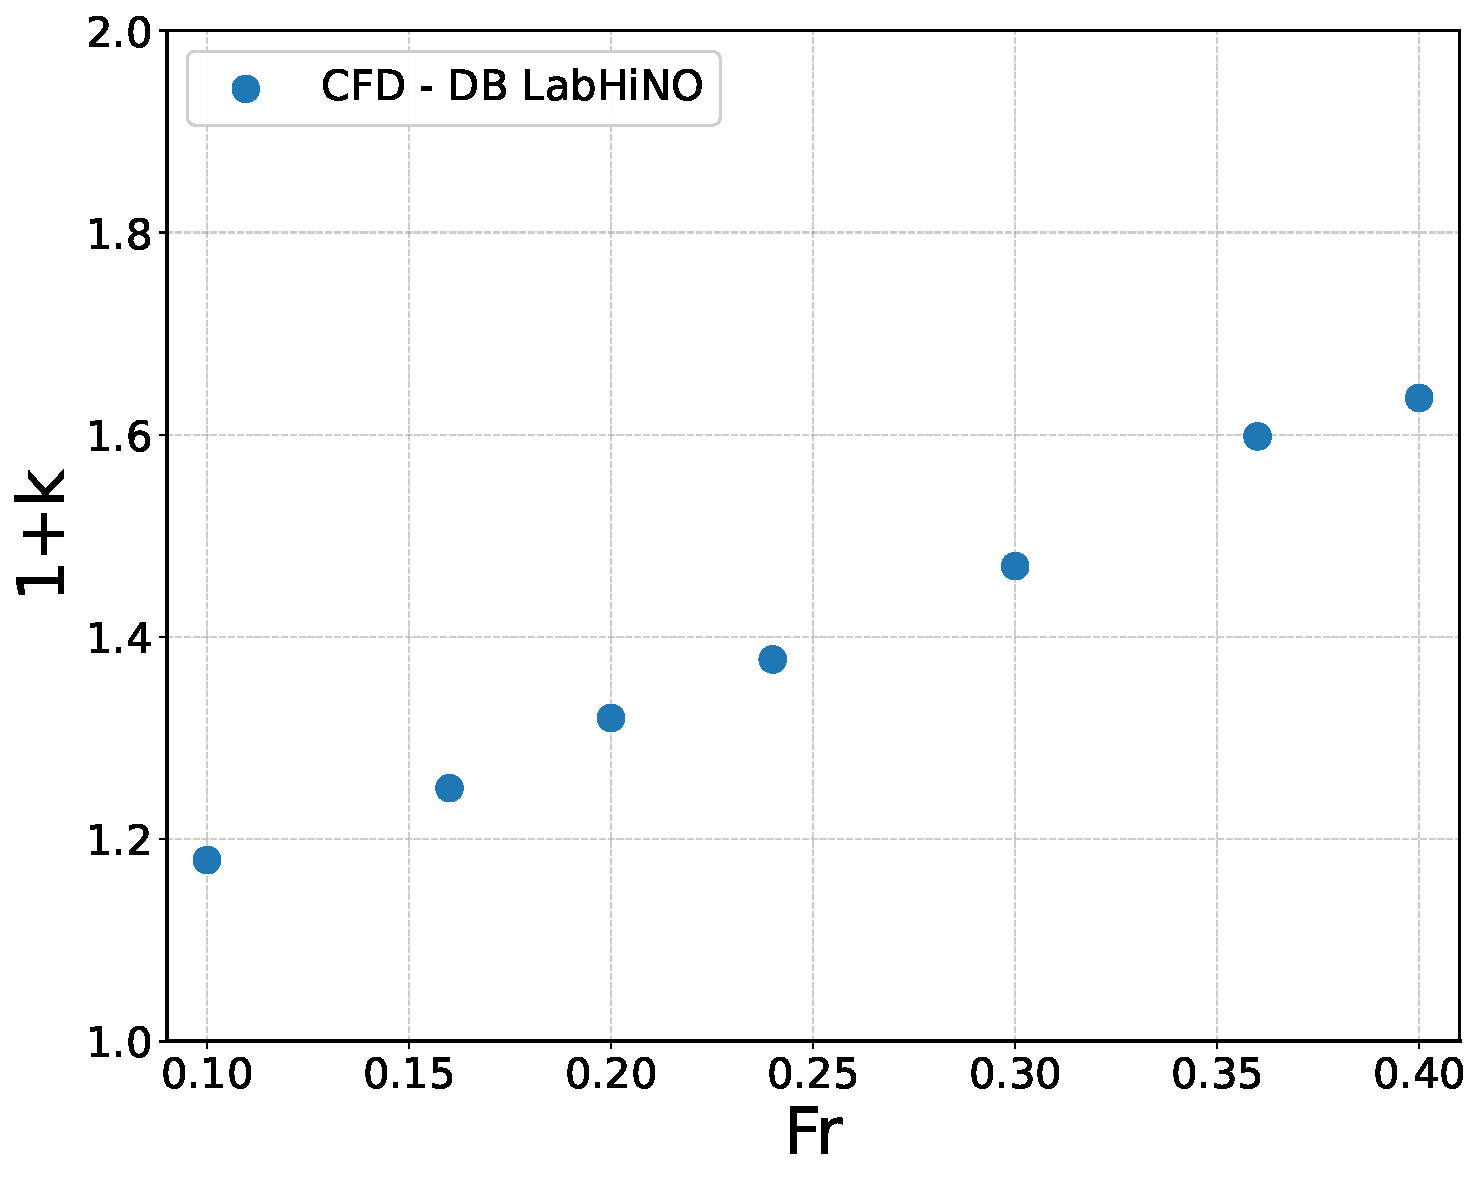
\includegraphics[width=\textwidth]{images/tpa_CFD_DB_195.pdf}
        \caption{Calado 3 (T3: 0.195 m)}
        \label{fig:k_195}
    \end{subfigure}

    \caption{Factor de forma calculado mediante el método de doble cuerpo para el \textit{P1} en los tres calados analizados, en función de Froude.}
    \label{fig:tpa_DB_k_evolucion}
\end{figure}

\subsubsection{Validación con modelo de referencia KCS}

Dada la variabilidad observada en el \textit{P1}, resulta necesario descartar 
que se trate de un error sistemático en la configuración del solver o del 
modelo de turbulencia. Para ello, se replicó exactamente la misma metodología 
sobre el modelo de referencia KCS (escala 1:79). La verificación numérica 
correspondiente se resume en la Tabla~\ref{tab:CFD_KCS}.

\begin{table}[htbp]
\centering
\caption{Verificación numérica para el modelo KCS a escala 1:79.}
\label{tab:CFD_KCS}
\small
\begin{tabular}{ccccc}
\toprule
\textbf{Fr} & \textbf{Re} & \boldmath{$y^+$} & \textbf{1+k} & \textbf{GCI [\%]} \\
\midrule
0.020 & $3.19\times10^{5}$ & 0.32 & 1.015 & 0.12 \\
0.040 & $6.37\times10^{5}$ & 0.91 & 1.022 & 0.06 \\
0.060 & $9.56\times10^{5}$ & 1.70 & 1.039 & 0.04 \\
0.080 & $1.28\times10^{6}$ & 2.64 & 1.101 & 0.01 \\
0.100 & $1.59\times10^{6}$ & 3.71 & 1.141 & 0.09 \\
0.120 & $1.91\times10^{6}$ & 4.90 & 1.218 & 0.07 \\
0.140 & $2.23\times10^{6}$ & 6.21 & 1.308 & 0.00 \\
0.160 & $2.55\times10^{6}$ & 7.61 & 1.314 & 0.01 \\
0.180 & $2.87\times10^{6}$ & 9.12 & 1.289 & 0.01 \\
0.200 & $3.19\times10^{6}$ & 10.71 & 1.254 & 0.04 \\
0.220 & $3.51\times10^{6}$ & 12.39 & 1.214 & 0.08 \\
0.240 & $3.82\times10^{6}$ & 14.16 & 1.182 & 0.11 \\
0.260 & $4.14\times10^{6}$ & 16.00 & 1.154 & 0.13 \\
0.280 & $4.46\times10^{6}$ & 17.92 & 1.131 & 0.20 \\
0.300 & $4.78\times10^{6}$ & 19.92 & 1.118 & 0.09 \\
0.320 & $5.10\times10^{6}$ & 21.98 & 1.118 & 0.43 \\
0.340 & $5.42\times10^{6}$ & 24.12 & 1.117 & 0.35 \\
0.360 & $5.74\times10^{6}$ & 26.32 & 1.114 & 1.06 \\
0.380 & $6.06\times10^{6}$ & 28.59 & 1.118 & 1.86 \\
0.400 & $6.37\times10^{6}$ & 30.93 & 1.117 & 1.09 \\
\bottomrule
\end{tabular}
\end{table}

A diferencia del \textit{P1}, el $y^+$ del KCS abarca desde la subcapa viscosa 
($y^+ \approx 0{.}3$) hasta el borde superior de la capa logarítmica 
($y^+ \approx 31$), atravesando la región \textit{buffer}. Pese a ello, la 
curva de $(1+k)$ resulta suave y sin cambios de pendiente, y el GCI se 
mantiene por debajo del $2\%$ en todo el rango. Esta robustez frente al 
tratamiento de pared se explica por la reducida contribución de la presión 
viscosa en este casco esbelto: al ser $C_{PV}$ una fracción pequeña de la 
resistencia viscosa total, el factor de forma queda dominado por $C_F$ y es 
poco sensible a la resolución de pared, en contraste con el \textit{P1}, donde 
$C_{PV}$ es comparable a $C_F$ (Sección~\ref{sec:descomposicion_de_la_res_viscosa}).

La Figura~\ref{fig:kcs_DB_prohaska} compara los resultados obtenidos con los 
reportados por \citet{TERZIEV2021147}. La concordancia es excelente, 
reproduciendo incluso la joroba característica en el rango de transición 
($Re \approx 10^6 - 3\times10^6$). Las líneas punteadas verticales indican 
los límites del rango de Froude recomendado por la ITTC para la aplicación 
del método de Prohaska ($Fr = 0.10$ y $Fr = 0.20$), correspondientes al 
modelo KCS a escala 1:79 ensayado en el LabHiNO, mientras que la línea 
horizontal continua representa el valor de $(1+k)$ adoptado a partir del 
ensayo experimental (EFD Prohaska, LabHiNO). Se observa que el valor 
experimental se ubica por debajo de los resultados CFD DB en ese rango, 
lo cual es consistente con la curvatura cóncava observada en el diagrama 
de Prohaska para las simulaciones numéricas, discutida en la 
Sección~\ref{sec:det_num_fac_form}.

\begin{figure}[htpb]
    \centering
    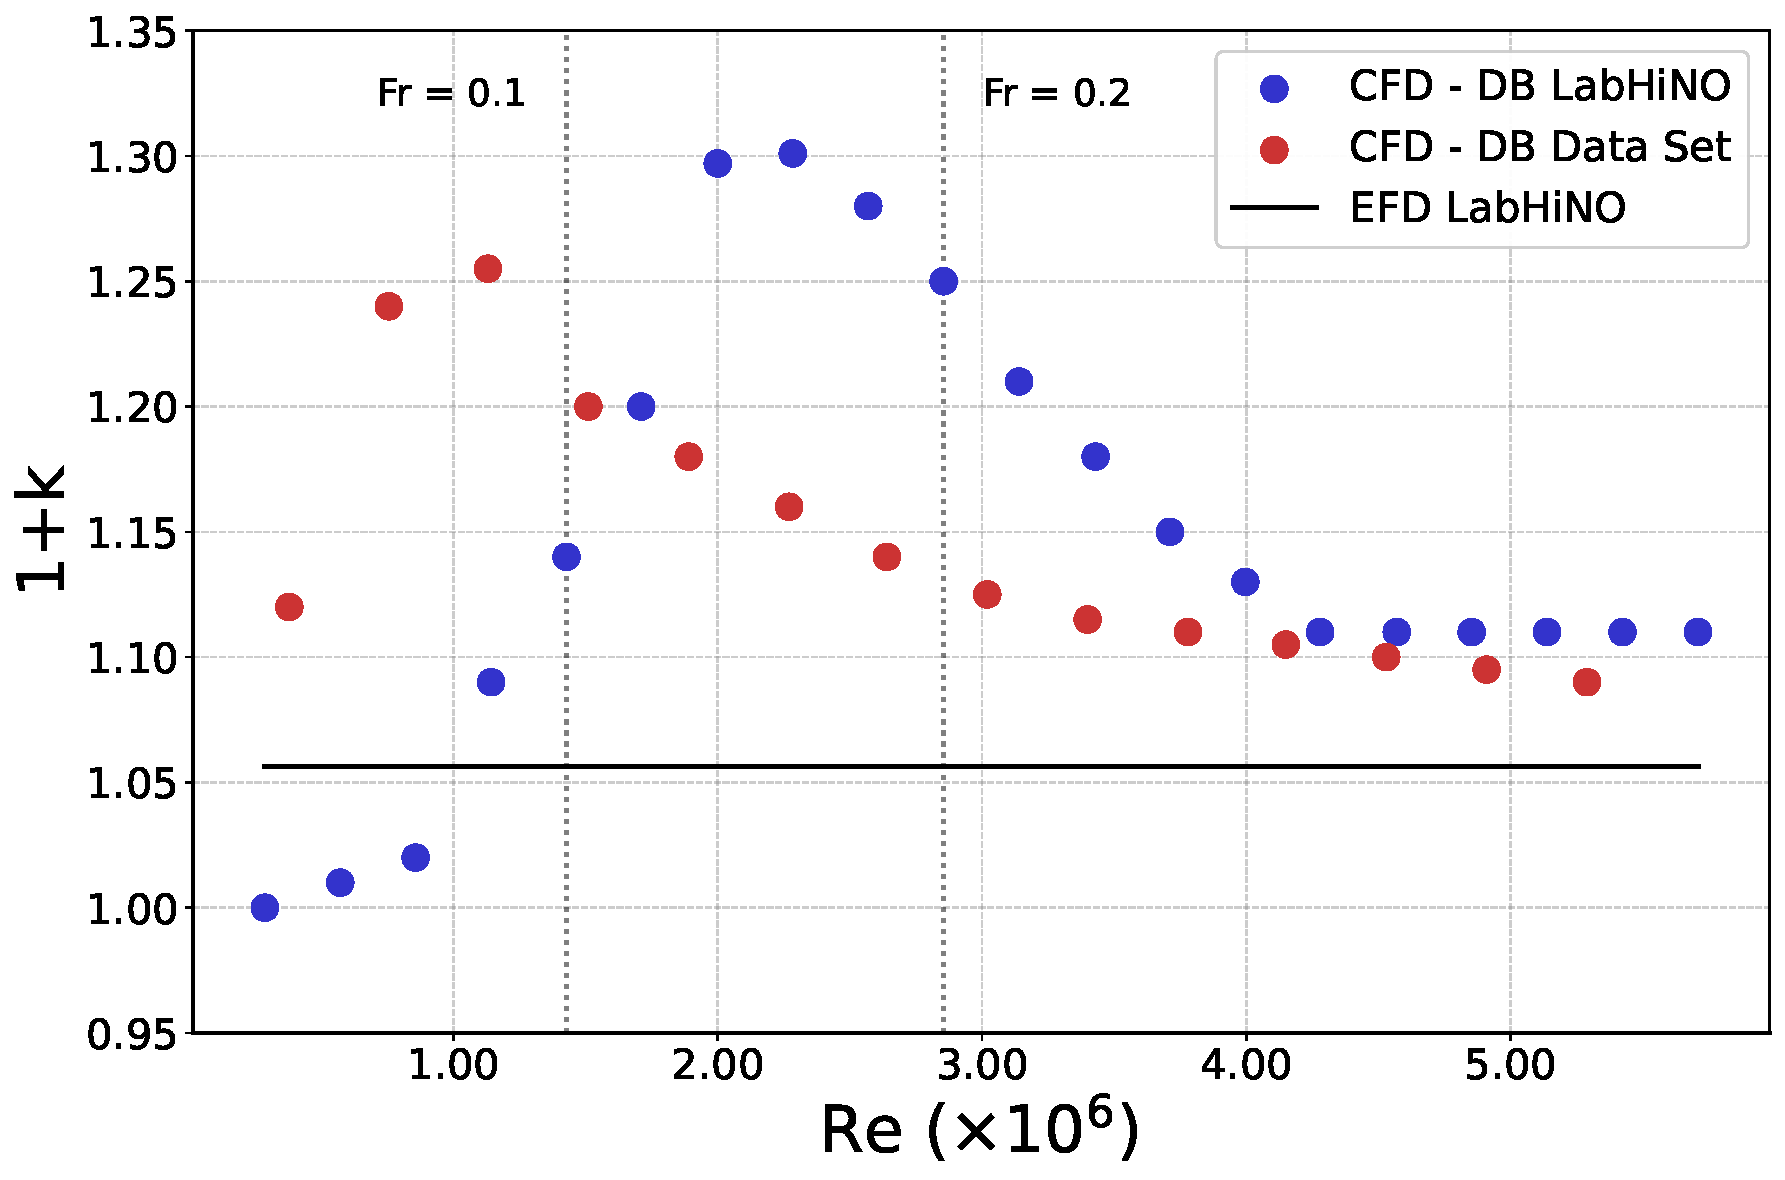
\includegraphics[width=.6\columnwidth]
        {images/kcs_DB_prohaska.pdf}
    \caption{Comparación de $1+k$ numérico vs $Re$ para el KCS 1:79 (escala LabHiNO) y 1:75 \citep{TERZIEV2021147}.}
    \label{fig:kcs_DB_prohaska}
\end{figure}

Finalmente, la Figura~\ref{fig:completo_kcs_lit} confirma que los resultados 
siguen la tendencia asintótica global validada por múltiples laboratorios 
internacionales \citep{TerzievDataSet}.

\begin{figure}[htpb]
    \centering
    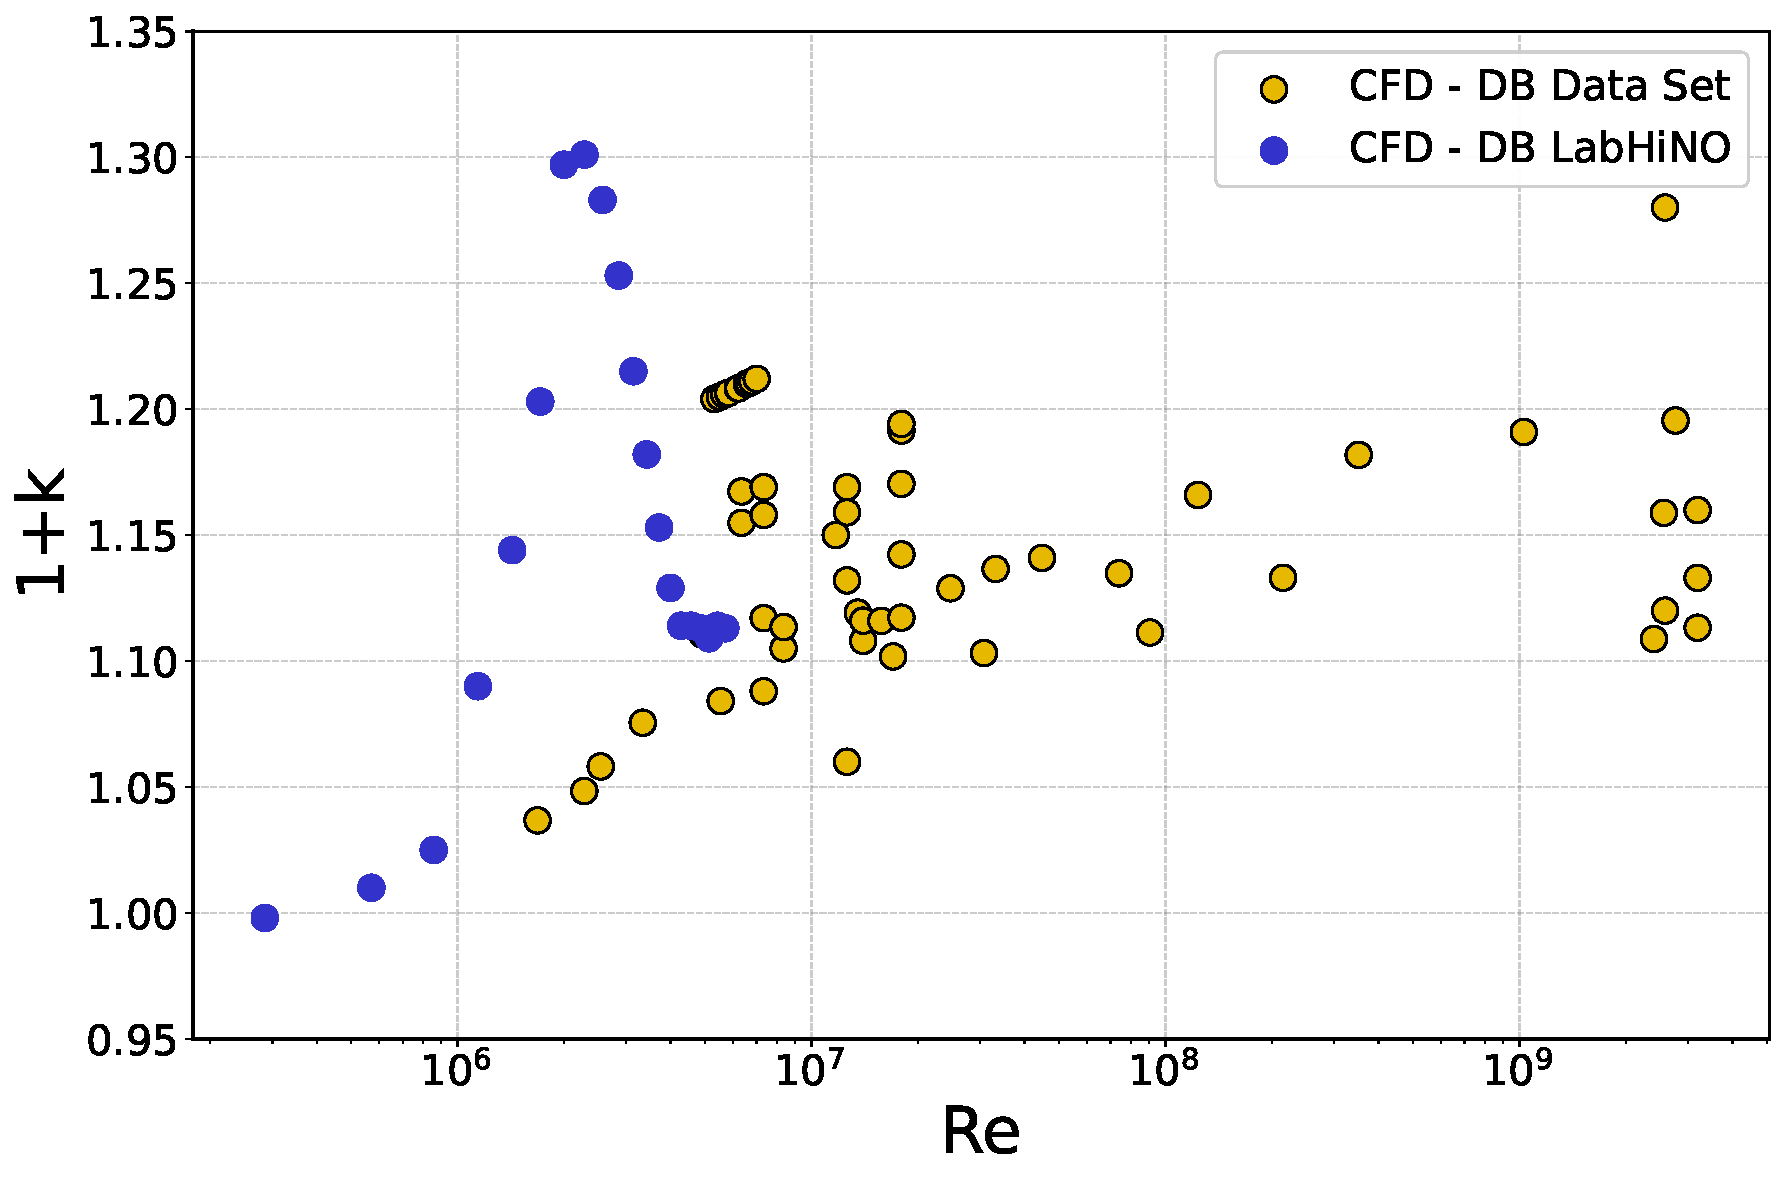
\includegraphics[width=.6\columnwidth]{images/cfd_kcs_lit.pdf}
    \caption{Factor de forma $(1+k)$ del KCS propio (CFD DB) frente a la base de datos \citep{TerzievDataSet}.}
    \label{fig:completo_kcs_lit}
\end{figure}

Esta validación cruzada permite afirmar que:
\begin{enumerate}
    \item La metodología numérica es correcta y precisa.
    \item La falta de estabilidad asintótica observada en el \textit{P1} no 
    es un error numérico ni un artefacto de la configuración del solver o del 
    modelo de turbulencia, sino una característica propia del casco analizado, 
    cuyo origen físico se analiza en profundidad en las secciones siguientes.
\end{enumerate}

\subsection{Comparación EFD CFD de resistencia y de factor de forma}

En esta sección se comparan los resultados experimentales y computacionales 
del \textit{P1} presentados en las secciones anteriores con el fin de 
sintetizar las diferencias encontradas. Esta comparación resulta central para 
el resto del análisis: dado que las simulaciones de doble cuerpo no admiten 
una validación experimental directa, al no existir un ensayo físico equivalente 
sin superficie libre, la confiabilidad del enfoque numérico completo descansa 
en la concordancia que aquí se establece entre el modelo bifásico con 
superficie libre y los ensayos de canal. Esta validación respalda, por 
extensión, la configuración numérica empleada (dominio, malla, modelo de 
turbulencia y condiciones de contorno) utilizada en las simulaciones de 
doble cuerpo presentadas en secciones posteriores.

\paragraph{Resistencia} Las Figuras~\ref{fig:resis_tpa_efd_cfd_165}
a~\ref{fig:resis_tpa_efd_cfd_195} comparan la resistencia experimental y
computacional del \textit{P1} para los tres calados. Para cuantificar
formalmente esta concordancia más allá de la inspección visual, se aplicó el
procedimiento de validación de la ITTC \citep{ITTC_uncertainty_CFD},
definiendo el error de comparación entre el valor experimental $D$ y el
numérico $S$ como $E\%D = (D-S)/D\times100$, y la incertidumbre de validación
como $U_{val}=\sqrt{U_D^2+U_{num}^2}$, con $U_D$ la incertidumbre experimental
(Tabla~\ref{tab:uncert_tpa}) y $U_{num}$ la numérica derivada del GCI. La
solución se considera validada, dentro de la incertidumbre disponible, cuando
$|E\%D|\le U_{val}$.

La validación formal se presenta para el Calado~2
(Tabla~\ref{tab:validacion_efd_cfd}), cuyos ensayos y simulaciones cubren el
rango operativo con una grilla de velocidades coincidente. El error de
comparación se mantiene dentro de la incertidumbre de medición hasta
$Fr \approx 0{.}26$, con un valor medio del orden del $1{.}5\%$ en ese
intervalo. A partir de $Fr \approx 0{.}29$ el modelo numérico subestima la
resistencia de manera creciente; esta desviación es atribuible a la
restricción de grados de libertad del modelo numérico —fijo en cabeceo y
hundimiento, frente al modelo libre del ensayo— y no a un error del modelo
físico, y ocurre además fuera del rango de operación del \textit{P1}. Los
puntos de $Fr < 0{.}18$ se excluyen del análisis por la baja relación
señal--ruido característica del régimen de baja resistencia.

\begin{table}[htbp]
\centering
\caption{Validación EFD--CFD de la resistencia total del \textit{P1}
(Calado~2, $T=0{.}180$~m) en el rango operativo. Error de comparación
$E\%D=(D-S)/D\times100$; incertidumbre de validación
$U_{val}=\sqrt{U_D^2+U_{num}^2}\approx U_D$, siendo $U_{num}<0{.}2\%$
despreciable frente a $U_D$ en este rango.}
\label{tab:validacion_efd_cfd}
\small
\begin{tabular}{ccccc}
\toprule
\textbf{Fr} & \boldmath{$E\%D$ [\%]} & \boldmath{$U_D$ [\%]} &
\boldmath{$U_{val}$ [\%]} & \textbf{¿Validado?} \\
\midrule
0.20 & $-2{.}4$ & 3.7 & 3.7 & Sí \\
0.22 & $-0{.}1$ & 3.1 & 3.1 & Sí \\
0.24 & $\phantom{-}1{.}3$ & 2.6 & 2.6 & Sí \\
0.26 & $\phantom{-}1{.}0$ & 2.0 & 2.0 & Sí \\
0.29 & $\phantom{-}4{.}1$ & 1.7 & 1.7 & No \\
0.32 & $\phantom{-}4{.}7$ & 1.4 & 1.4 & No \\
\bottomrule
\end{tabular}
\end{table}

El mismo análisis se aplicó a los calados restantes. Para el Calado~1
($T=0{.}165$~m), el error de comparación medio en el rango operativo es del
orden del $5\%$, mayor que en el Calado~2 y asociado a una mayor dispersión de
las corridas CFD en esa condición; aun así se mantiene dentro de márgenes
habituales para la predicción de resistencia por CFD. Para el Calado~3
($T=0{.}195$~m), los ensayos experimentales y las simulaciones se realizaron
sobre grillas de $Fr$ no coincidentes, por lo que la comparación se efectúa
interpolando la curva CFD a las velocidades ensayadas; sobre los puntos
comparables del rango operativo, la concordancia entre las curvas experimental
y computacional es del orden del $1$--$2\%$, consistente con la obtenida para
los demás calados.

En conjunto, la concordancia EFD--CFD en el rango operativo respalda la
confiabilidad del modelo numérico con superficie libre y, por extensión, de
las simulaciones de doble cuerpo, que carecen de contrapartida experimental
directa (Sección~\ref{sec:4.1.5_enfoque_doble_cuerpo}).

\begin{figure}[htpb]
     \centering
     \begin{subfigure}[b]{0.45\textwidth}
         \centering
         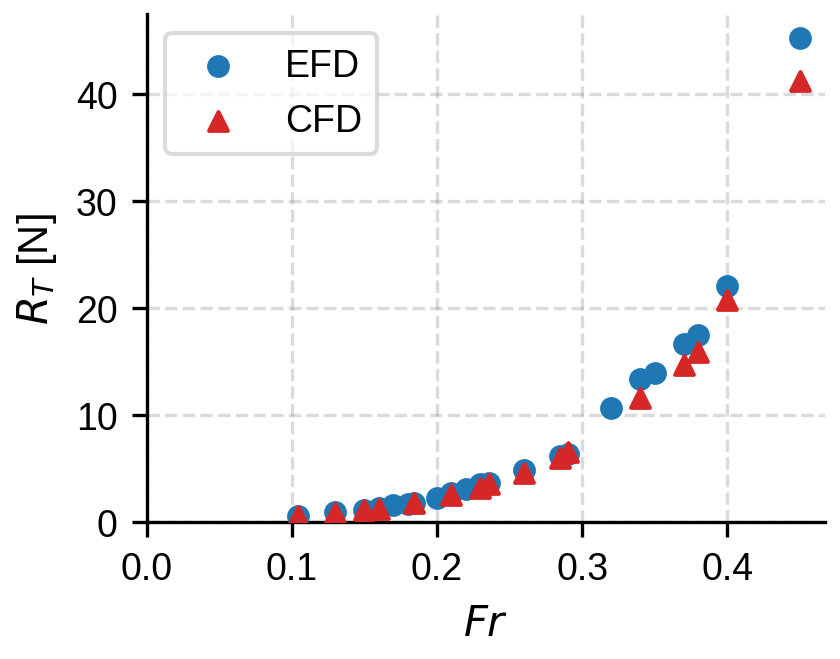
\includegraphics[width=\textwidth]{images/efd-cfd-165}
         \caption{Calado 1.}
         \label{fig:resis_tpa_efd_cfd_165}
     \end{subfigure}
     \hfill
     \begin{subfigure}[b]{0.45\textwidth}
         \centering
         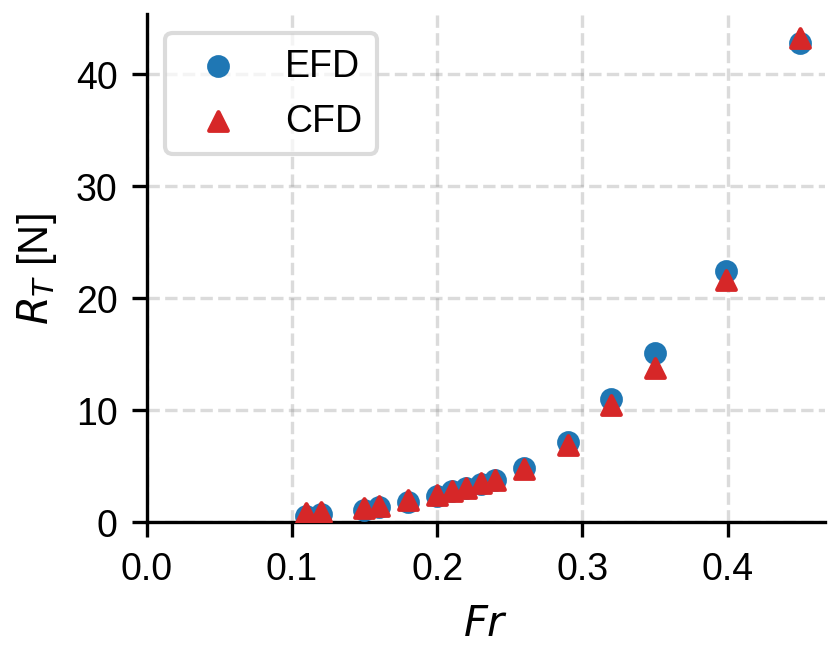
\includegraphics[width=\textwidth]{images/efd-cfd-180}
         \caption{Calado 2.}
         \label{fig:resis_tpa_efd_cfd_180}
     \end{subfigure}

     \vspace{0.5cm}

     \begin{subfigure}[b]{0.45\textwidth}
         \centering
         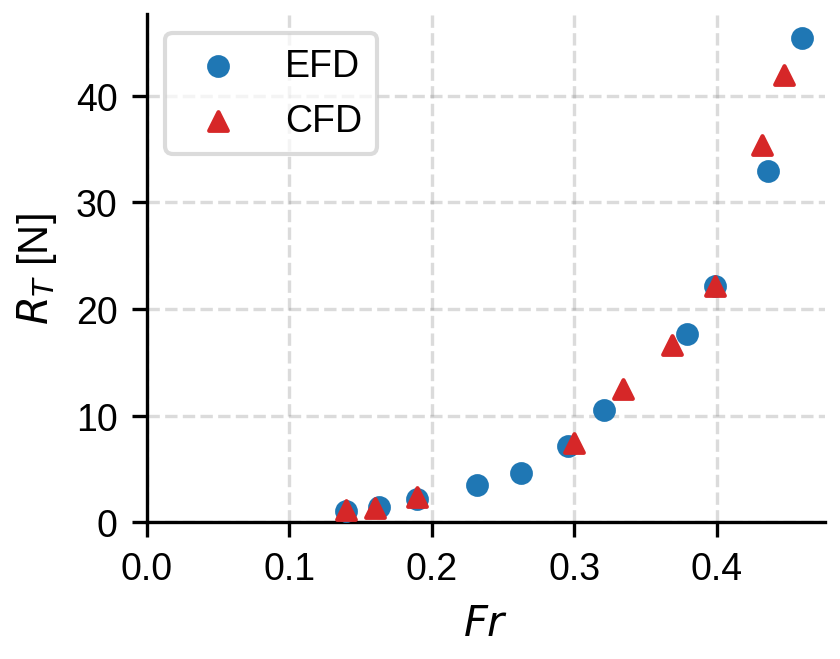
\includegraphics[width=\textwidth]{images/efd-cfd-195}
         \caption{Calado 3.}
         \label{fig:resis_tpa_efd_cfd_195}
     \end{subfigure}

     \caption{Resistencia al avance del \textit{P1} en función de $Fr$. 
     Comparación EFD--CFD para los tres calados.}
     \label{fig:comparativa_efd_cfd_calados}
\end{figure}

\paragraph{Factor de forma} Como fue mencionado en las secciones 
\ref{sec:det_exp_fac_form} y \ref{sec:det_num_fac_form}, tanto para el cálculo 
experimental como para el computacional, no es posible ajustar adecuadamente 
la recta esperada por el método de Prohaska a bajas velocidades. Las 
Figuras~\ref{fig:prohaska_tpa_efd_cfd_165} a \ref{fig:prohaska_tpa_efd_cfd_195} 
superponen los diagramas de Prohaska del \textit{P1} obtenidos mediante EFD 
(recta D2) y CFD (recta D1) para cada calado, junto con los puntos 
correspondientes a cada enfoque. Ambas rectas representan la extrapolación 
lineal sobre el rango $0.10 < Fr < 0.20$, cuya ordenada al origen determina 
el valor de $(1+k)$ adoptado en cada caso. Se observa que las rectas EFD y 
CFD se cruzan en un punto intermedio del rango analizado, lo que indica que 
la desviación respecto de la linealidad teórica tiene signo opuesto en ambos 
enfoques: mientras que los puntos experimentales tienden a curvarse de forma 
convexa, los puntos numéricos lo hacen de forma cóncava. Como se discutió en 
la Sección~\ref{sec:prohaska_antec}, esta desviación puede atribuirse a 
múltiples causas, entre ellas la laminarización parcial del flujo, la 
geometría de la proa bulbo, la separación de flujo en popa y el sesgo 
introducido por la línea de correlación ITTC-1957. En el caso particular de 
las simulaciones CFD, la curvatura cóncava observada es consistente con la 
incapacidad del modelo de turbulencia $k$-$\omega$ SST de reproducir 
correctamente la zona de transición a bajos $Re$.

\begin{figure}[htpb]
\centering
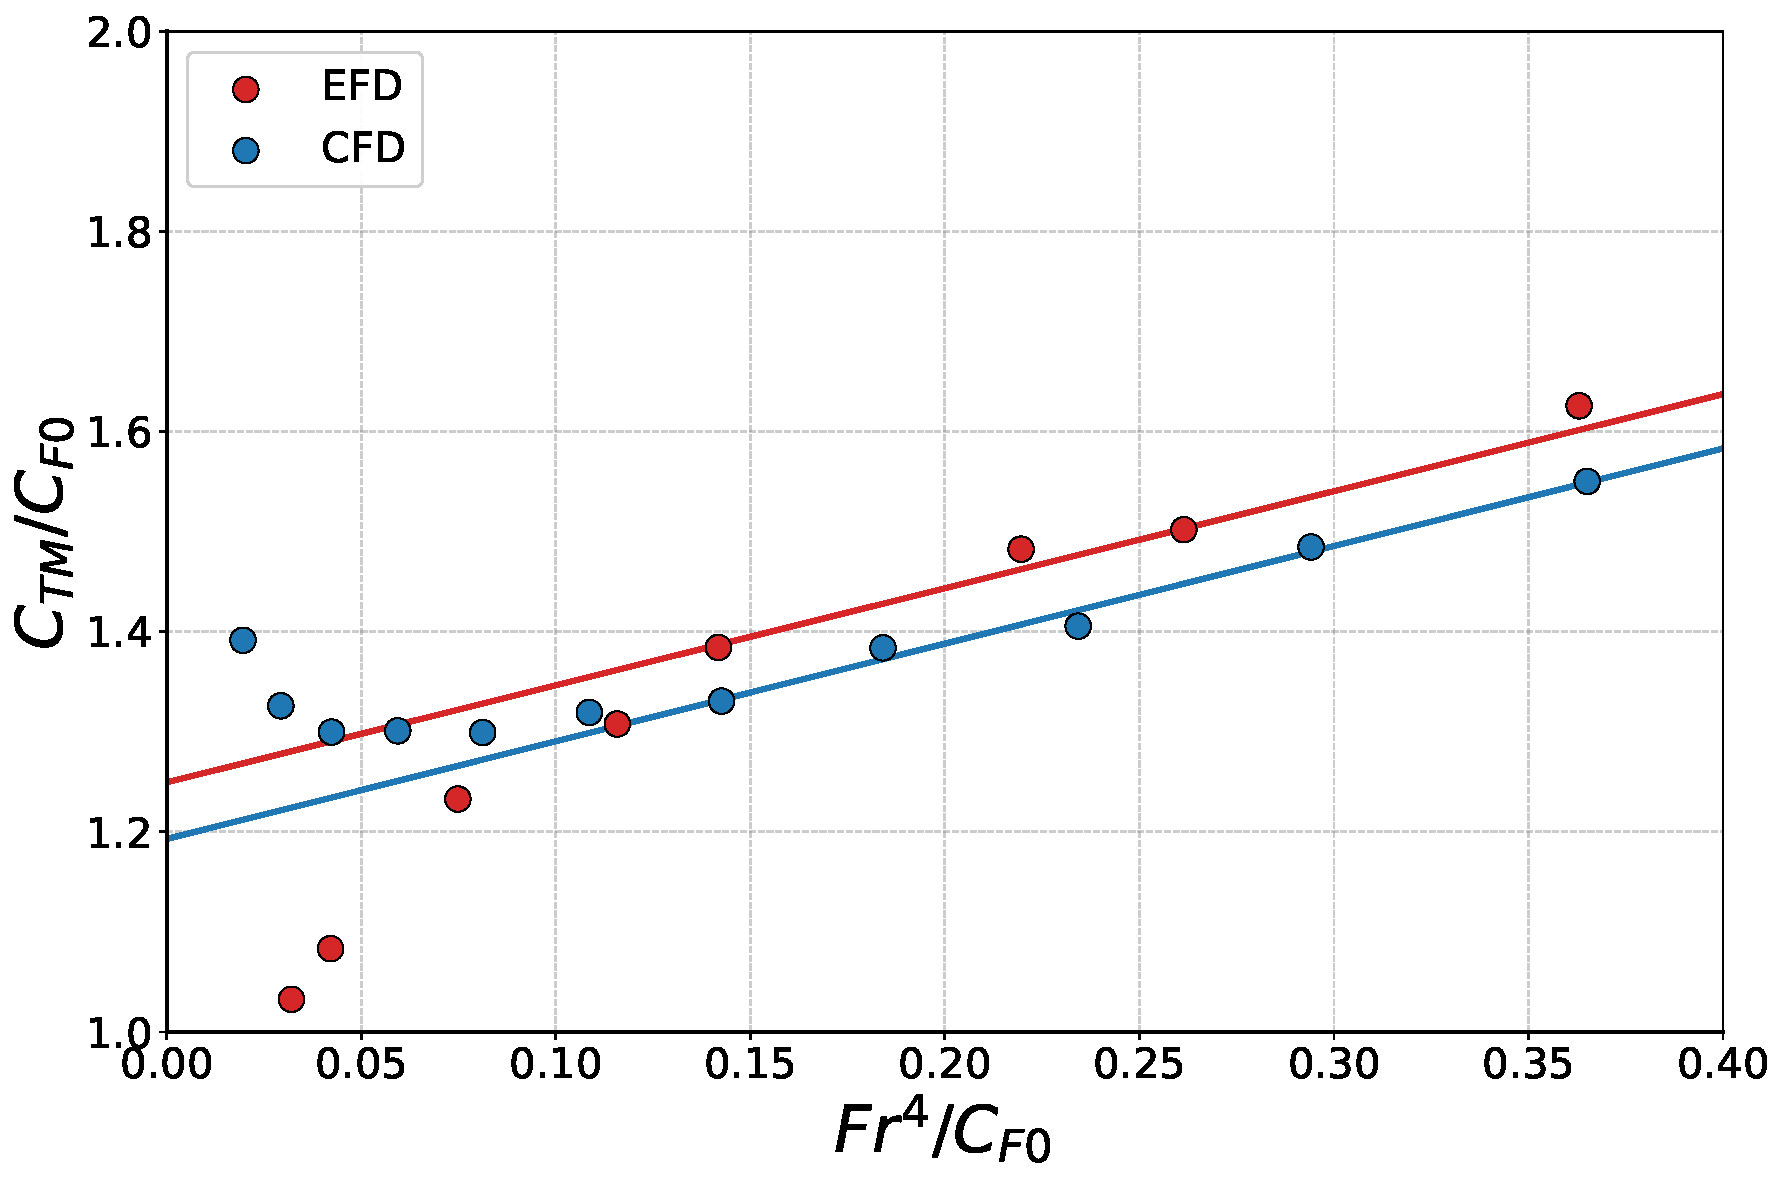
\includegraphics[width=0.6\textwidth]{images/prohaska-efd-cfd-165.pdf}
\caption{Diagrama de Prohaska del \textit{P1} comparando EFD y CFD. Calado 1.}
\label{fig:prohaska_tpa_efd_cfd_165}
\end{figure}

\begin{figure}[htpb]
\centering
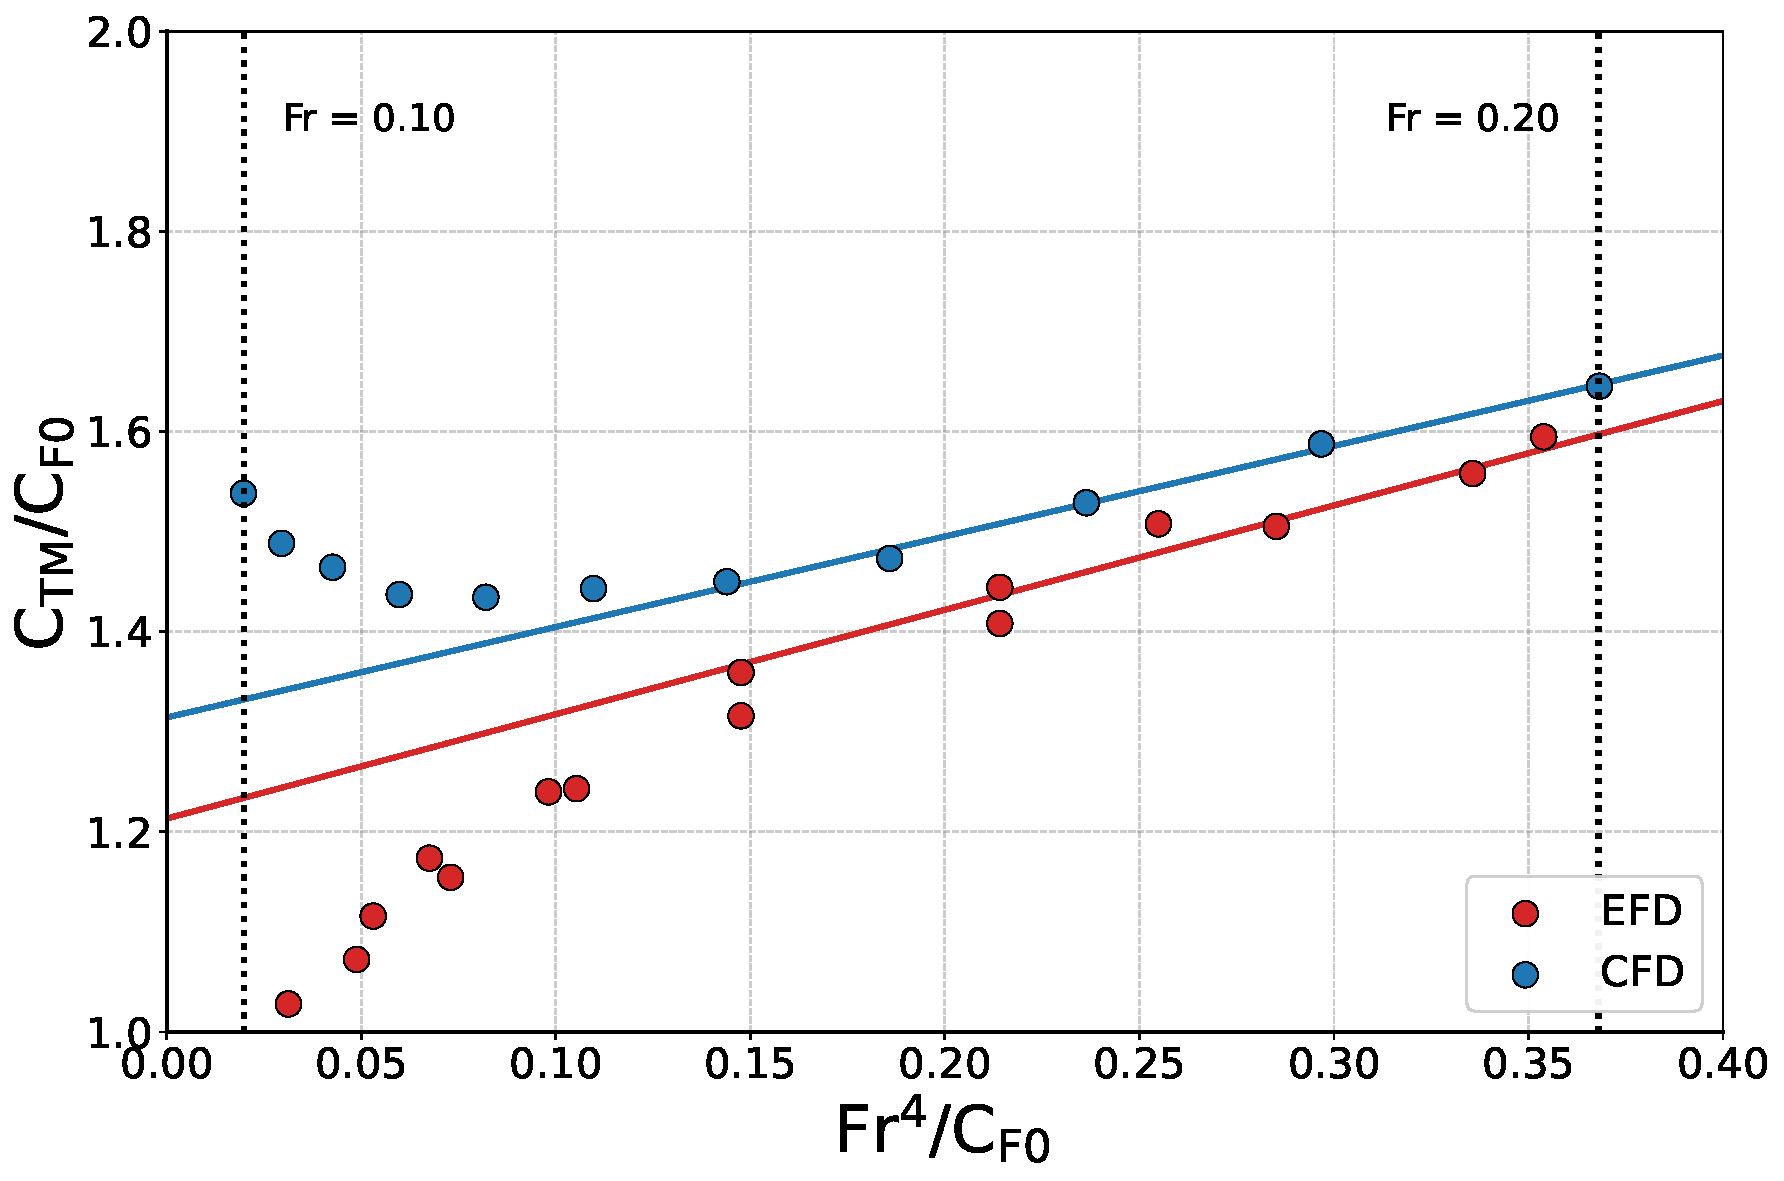
\includegraphics[width=0.6\textwidth]{images/prohaska-efd-cfd-180.pdf}
\caption{Diagrama de Prohaska del \textit{P1} comparando EFD y CFD. Calado 2.}
\label{fig:prohaska_tpa_efd_cfd_180}
\end{figure}

\begin{figure}[htpb]
\centering
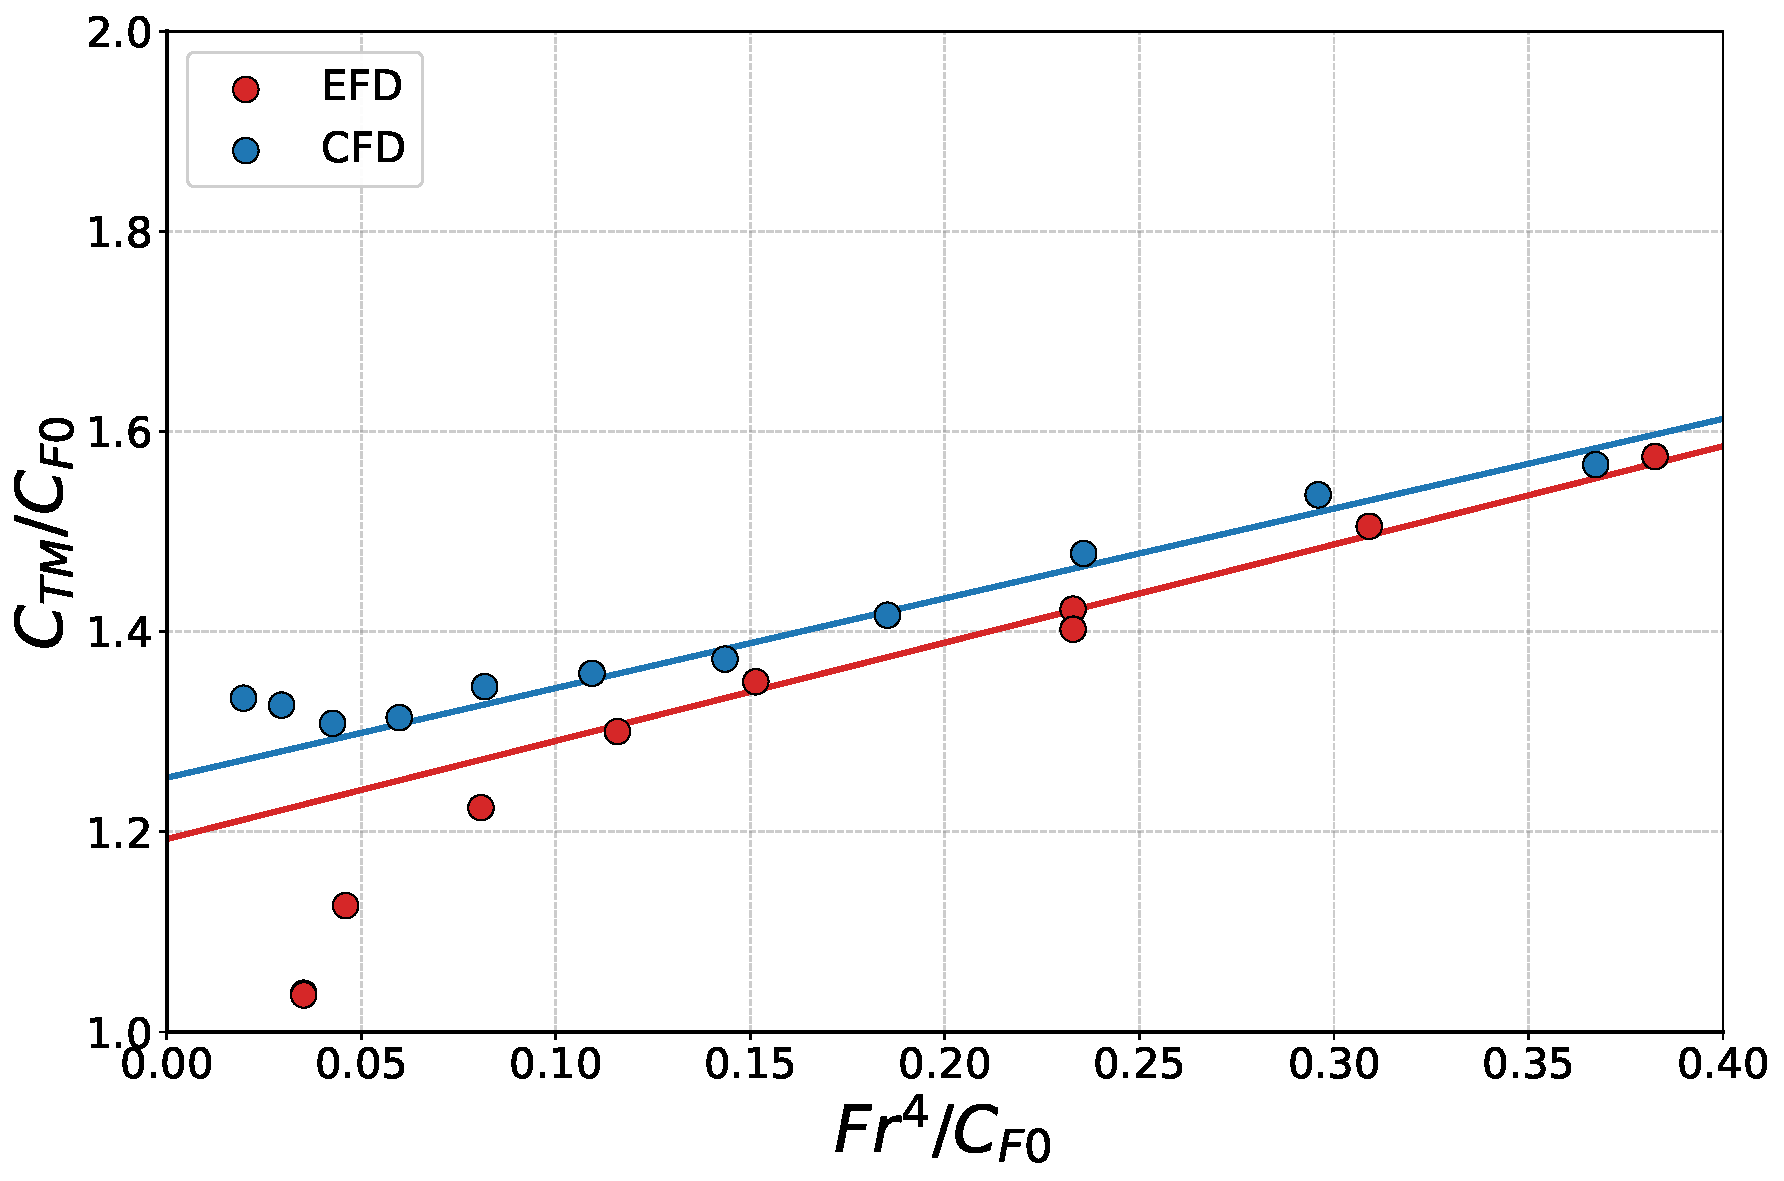
\includegraphics[width=0.6\textwidth]{images/prohaska-efd-cfd-195.pdf}
\caption{Diagrama de Prohaska del \textit{P1} comparando EFD y CFD. Calado 3.}
\label{fig:prohaska_tpa_efd_cfd_195}
\end{figure}

La Figura~\ref{fig:comparativa_form_factor_range} muestra, para cada calado, 
el valor de $(1+k)$ obtenido por Prohaska al variar el límite inferior del 
rango de Froude considerado en la regresión, tanto para EFD como para CFD. 
Se observa que, al restringir el rango a $0.13 < Fr < 0.18$ aproximadamente, 
ambos enfoques convergen a un valor prácticamente idéntico, eliminando la 
discrepancia inicial observada a bajas velocidades. Este resultado confirma 
que, dentro del rango adecuado de aplicación del método, tanto el ensayo 
experimental como la simulación numérica con superficie libre predicen el 
mismo factor de forma para el \textit{P1}.

\begin{figure}[htpb]
     \centering
     \begin{subfigure}[b]{0.48\textwidth}
         \centering
         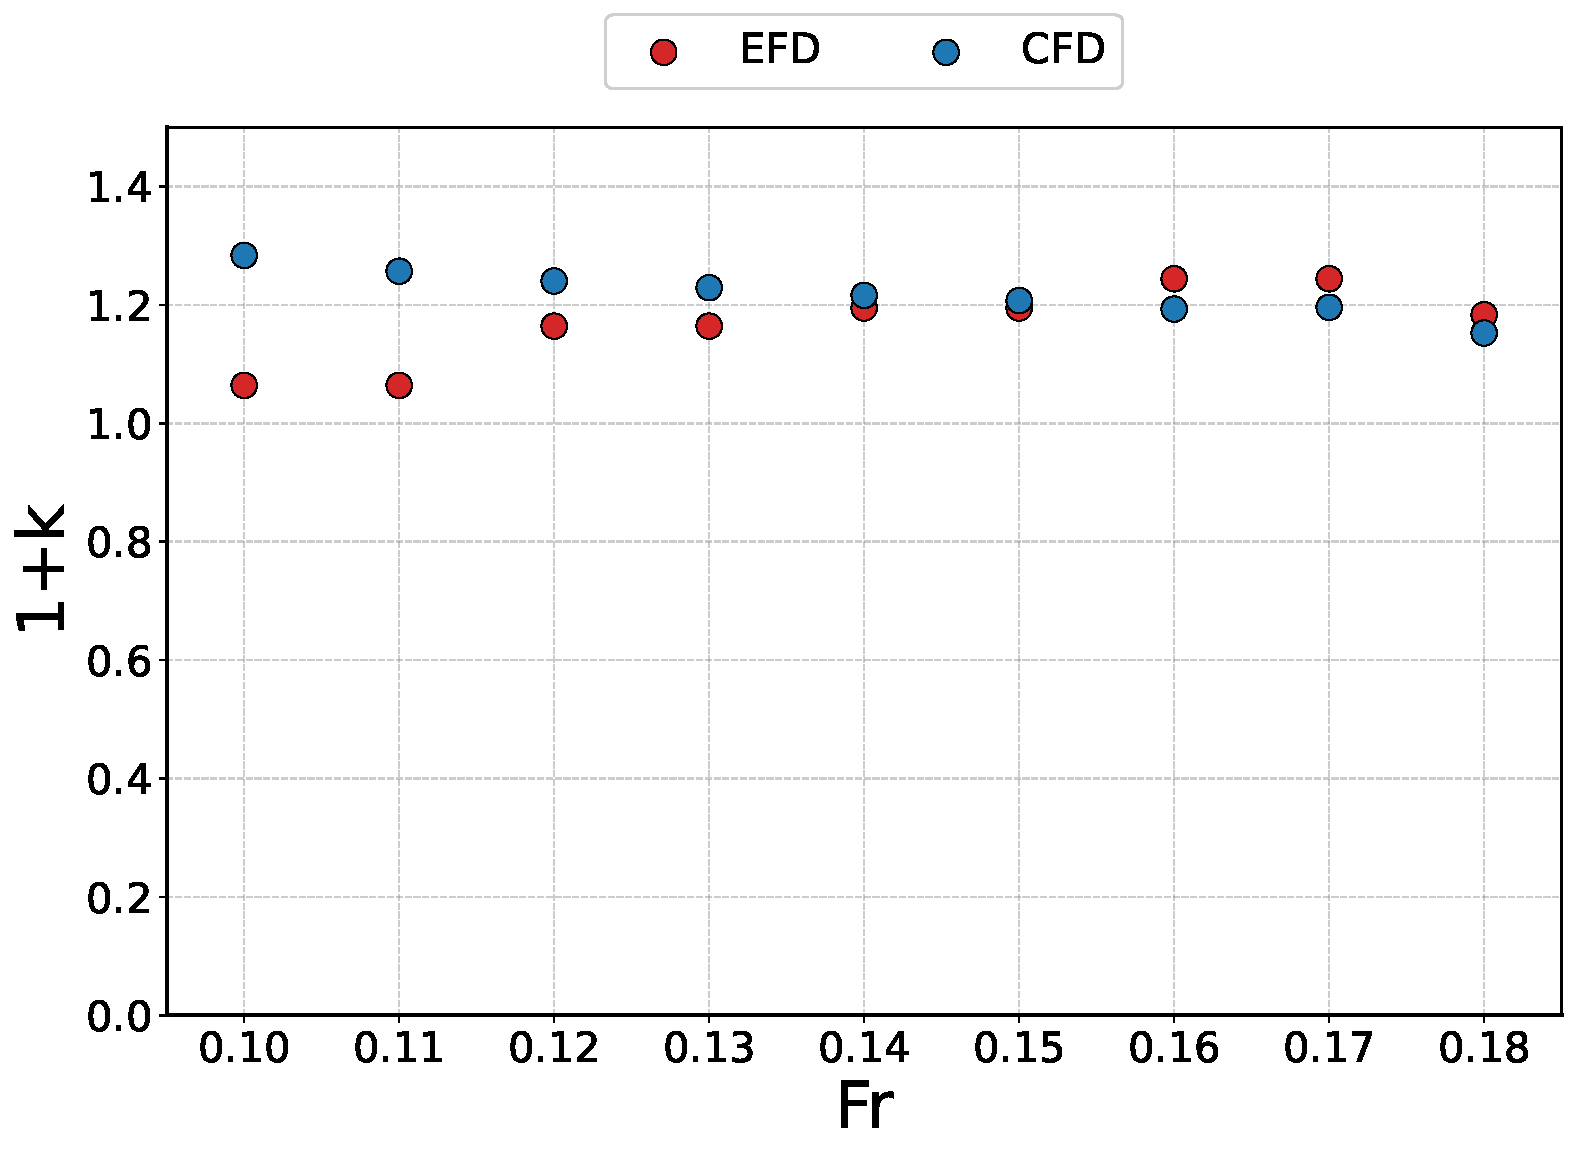
\includegraphics[width=\textwidth]{images/efd_cfd_form_factor_tpa_165_range}
         \caption{Calado 1.}
         \label{fig:efd_cfd_165_tpa_range}
     \end{subfigure}
     \hfill
     \begin{subfigure}[b]{0.48\textwidth}
         \centering
         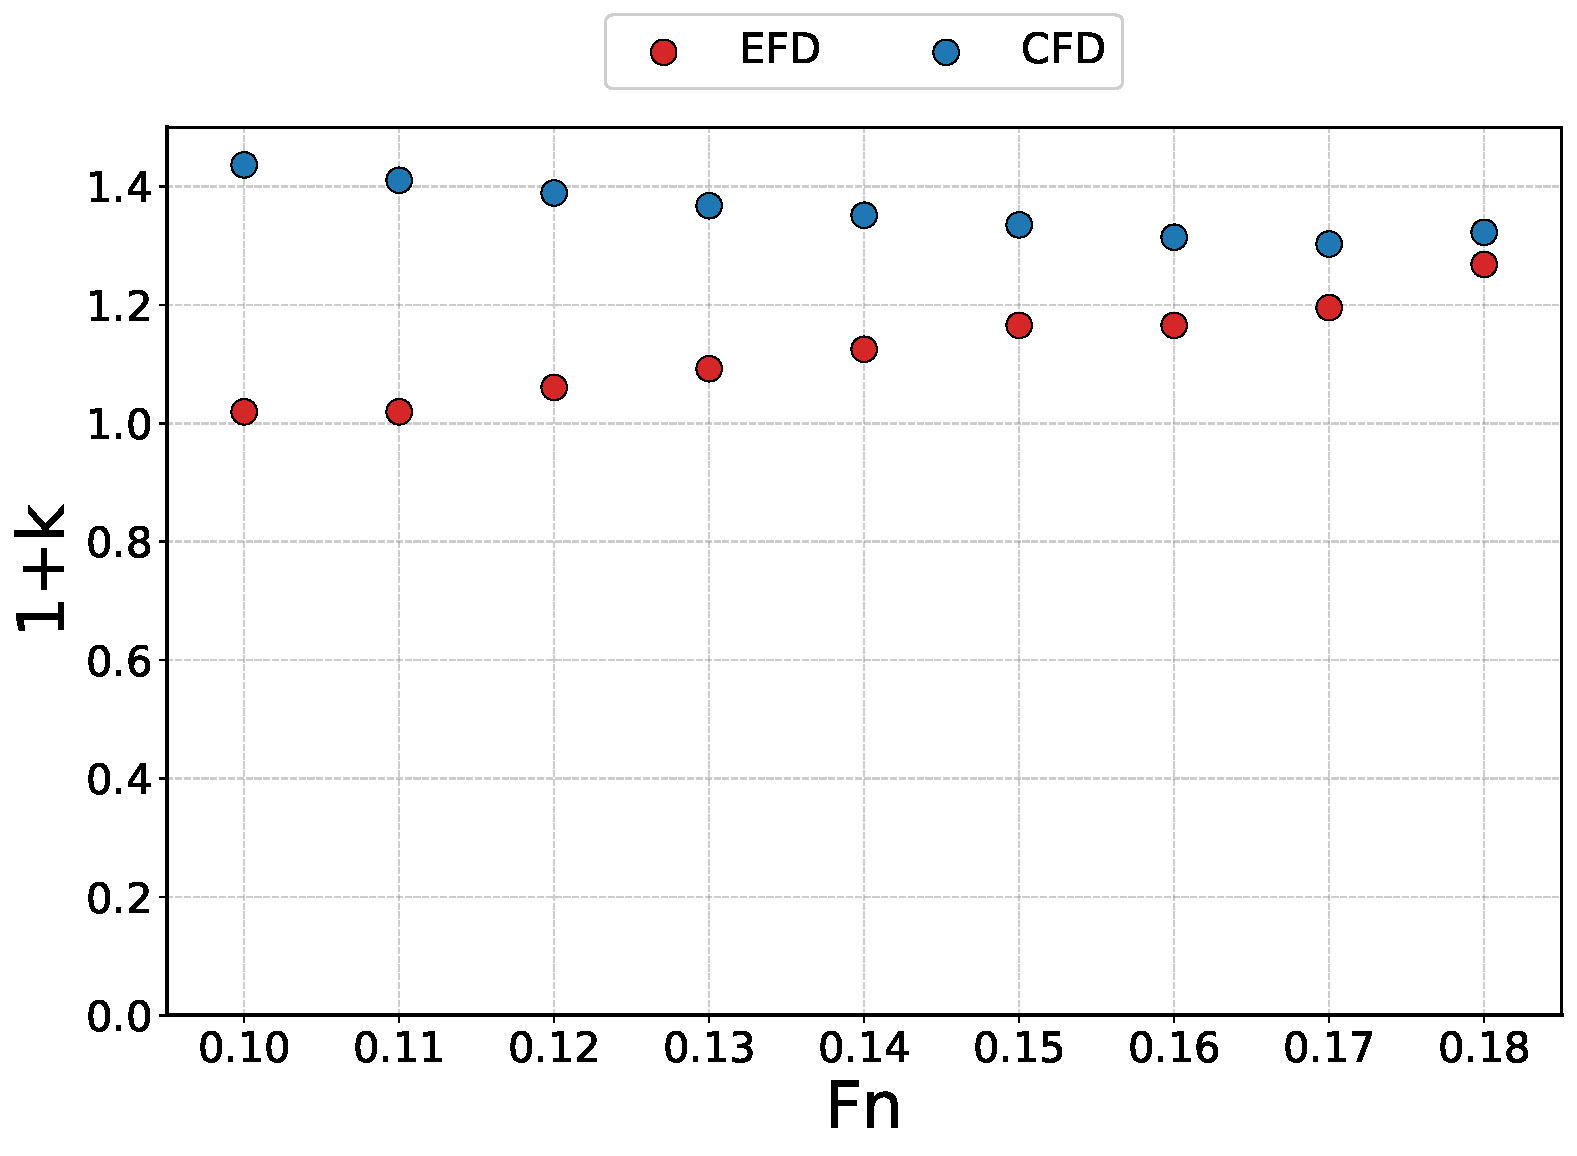
\includegraphics[width=\textwidth]{images/efd_cfd_form_factor_tpa_180_range}
         \caption{Calado 2.}
         \label{fig:efd_cfd_180_tpa_range}
     \end{subfigure}
     
     \vspace{0.5cm}
     
     \begin{subfigure}[b]{0.48\textwidth}
         \centering
         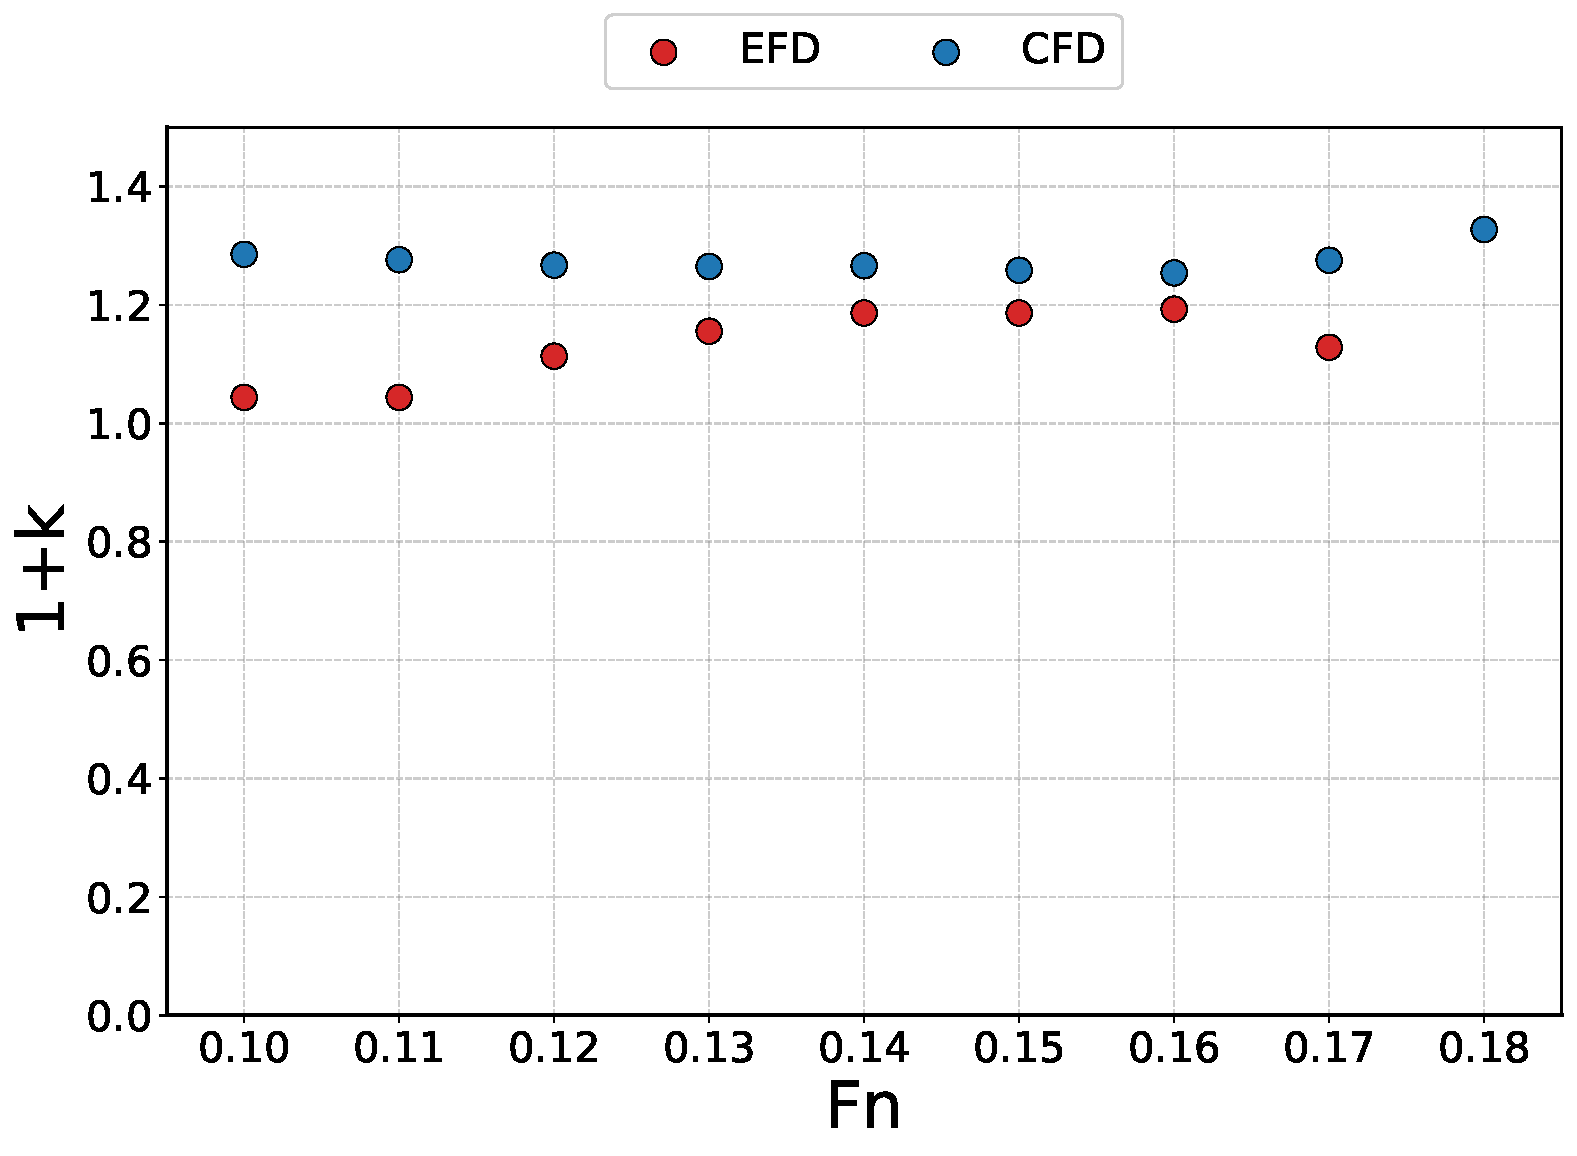
\includegraphics[width=\textwidth]{images/efd_cfd_form_factor_tpa_195_range}
         \caption{Calado 3.}
         \label{fig:efd_cfd_195_tpa_range}
     \end{subfigure}
     
     \caption{Variación del factor de forma $(1+k)$ del \textit{P1}, obtenido 
     mediante el método de Prohaska a partir de EFD y CFD, en función del 
     límite inferior del rango de Froude considerado en el ajuste.}
     \label{fig:comparativa_form_factor_range}
\end{figure}

Habiendo establecido un valor único y consistente de $(1+k)$ mediante Prohaska, 
surge la pregunta de cómo se relaciona este valor con los resultados obtenidos 
mediante el método de doble cuerpo, presentado en la 
Sección~\ref{sec:doble_cuerpo}. La Figura~\ref{fig:comparativa_doble_cuerpo} 
superpone, para cada calado, el valor adoptado por Prohaska (línea horizontal 
roja) con la evolución de $(1+k)$ obtenida mediante doble cuerpo en función 
de $Fr$ (puntos azules). Se observa que el valor de Prohaska coincide con los 
resultados de doble cuerpo específicamente en el rango $0.10 < Fr < 0.20$, es 
decir, el mismo rango utilizado para el ajuste de Prohaska. Sin embargo, para 
$Fr > 0.20$, el valor de doble cuerpo continúa creciendo de manera sostenida, 
mientras que el valor de Prohaska permanece constante por definición. Esto 
sugiere que el método de Prohaska, al restringirse a un rango acotado de bajas 
velocidades, podría estar capturando únicamente un punto particular de una 
curva de $(1+k)$ que en realidad varía con $Fr$ (o $Re$) en todo el rango 
operativo del buque, comportamiento que ya fue observado para el KCS y que 
será analizado en profundidad en la Sección~\ref{sec:analisis_efectos_escala}.

\begin{figure}[H]
     \centering
     \begin{subfigure}[b]{0.48\textwidth}
         \centering
         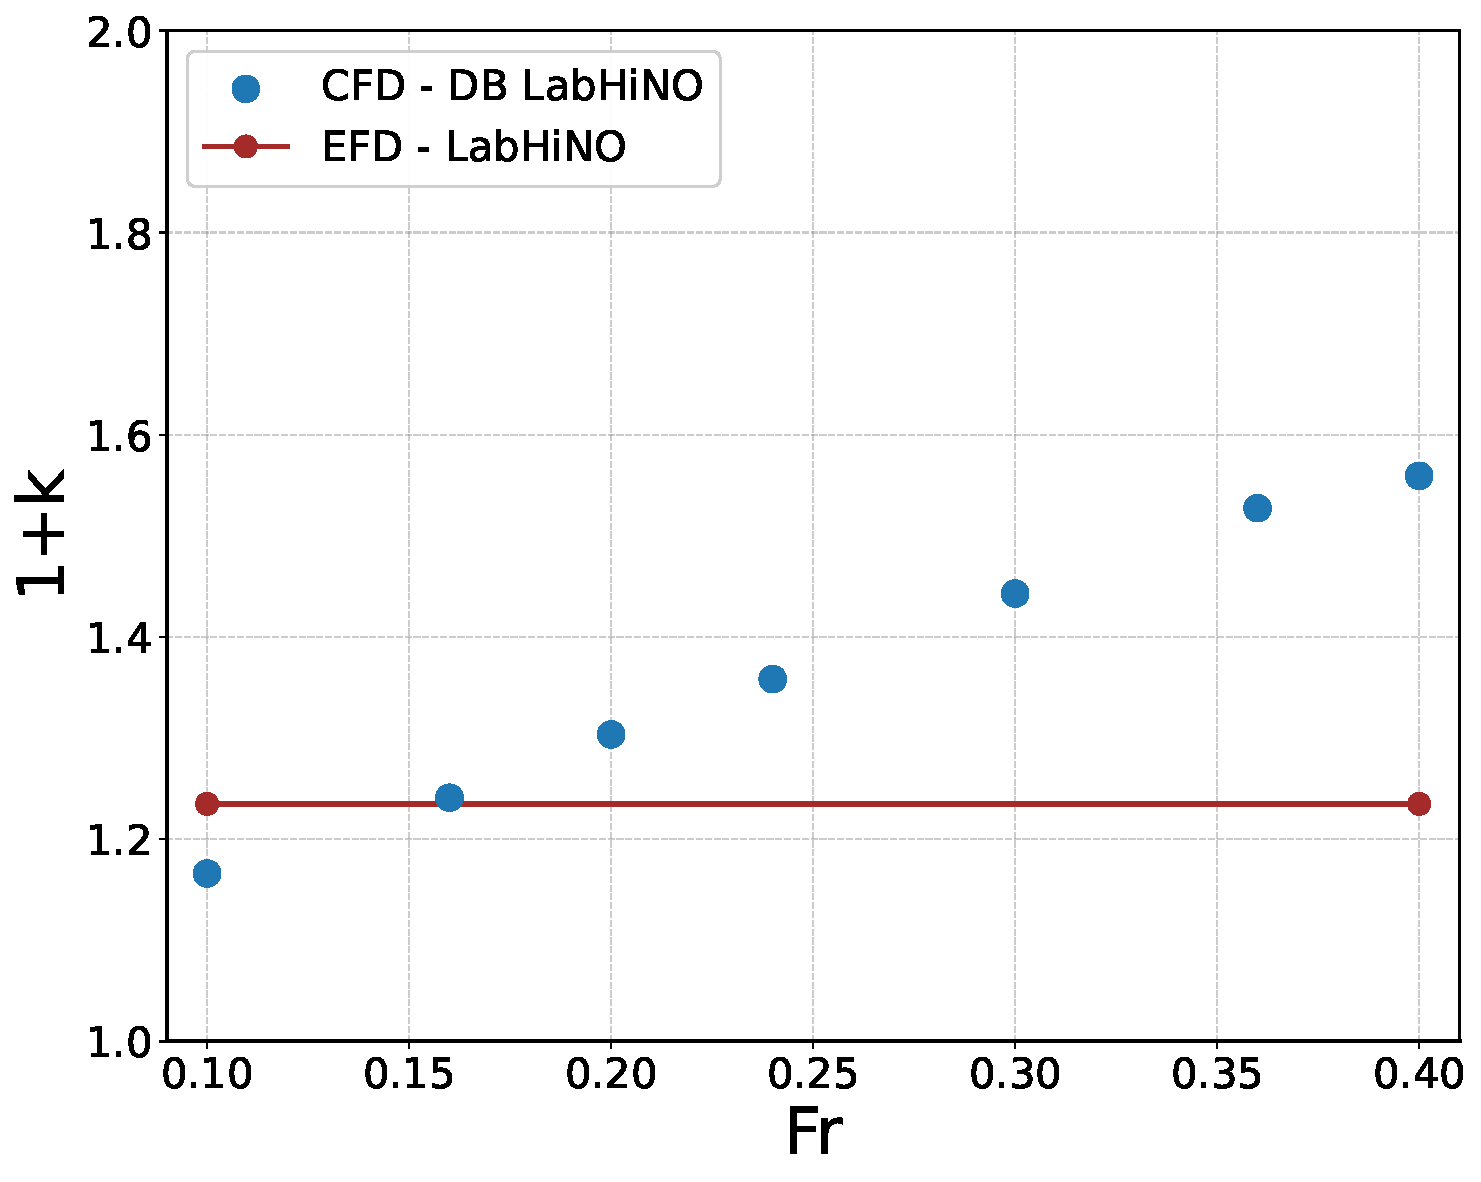
\includegraphics[width=\textwidth]{images/tpa_CFD_DB_prohaska_165.pdf}
         \caption{Calado 1.}
         \label{fig:tpa_proj_DB_k_escala20_165}
     \end{subfigure}
     \hfill
     \begin{subfigure}[b]{0.48\textwidth}
         \centering
         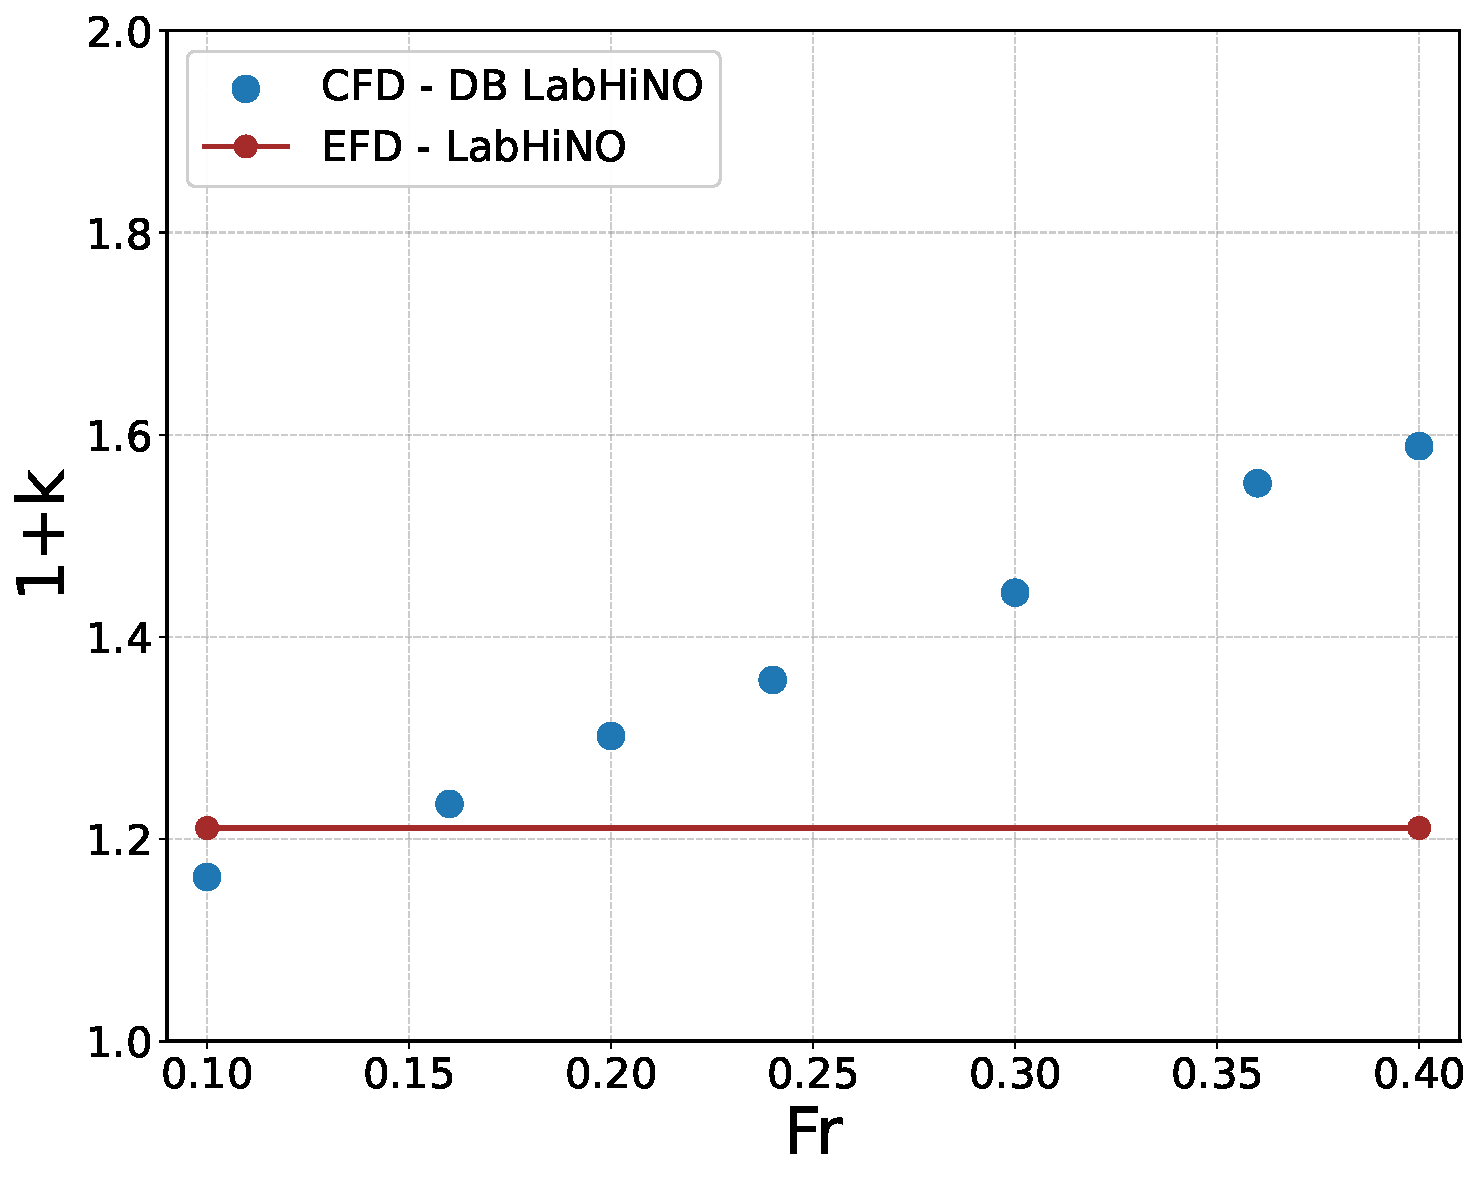
\includegraphics[width=\textwidth]{images/tpa_CFD_DB_prohaska_180.pdf}
         \caption{Calado 2.}
         \label{fig:tpa_proj_DB_k_escala20_180}
     \end{subfigure}
     
     \vspace{0.5cm}
     
     \begin{subfigure}[b]{0.48\textwidth}
         \centering
         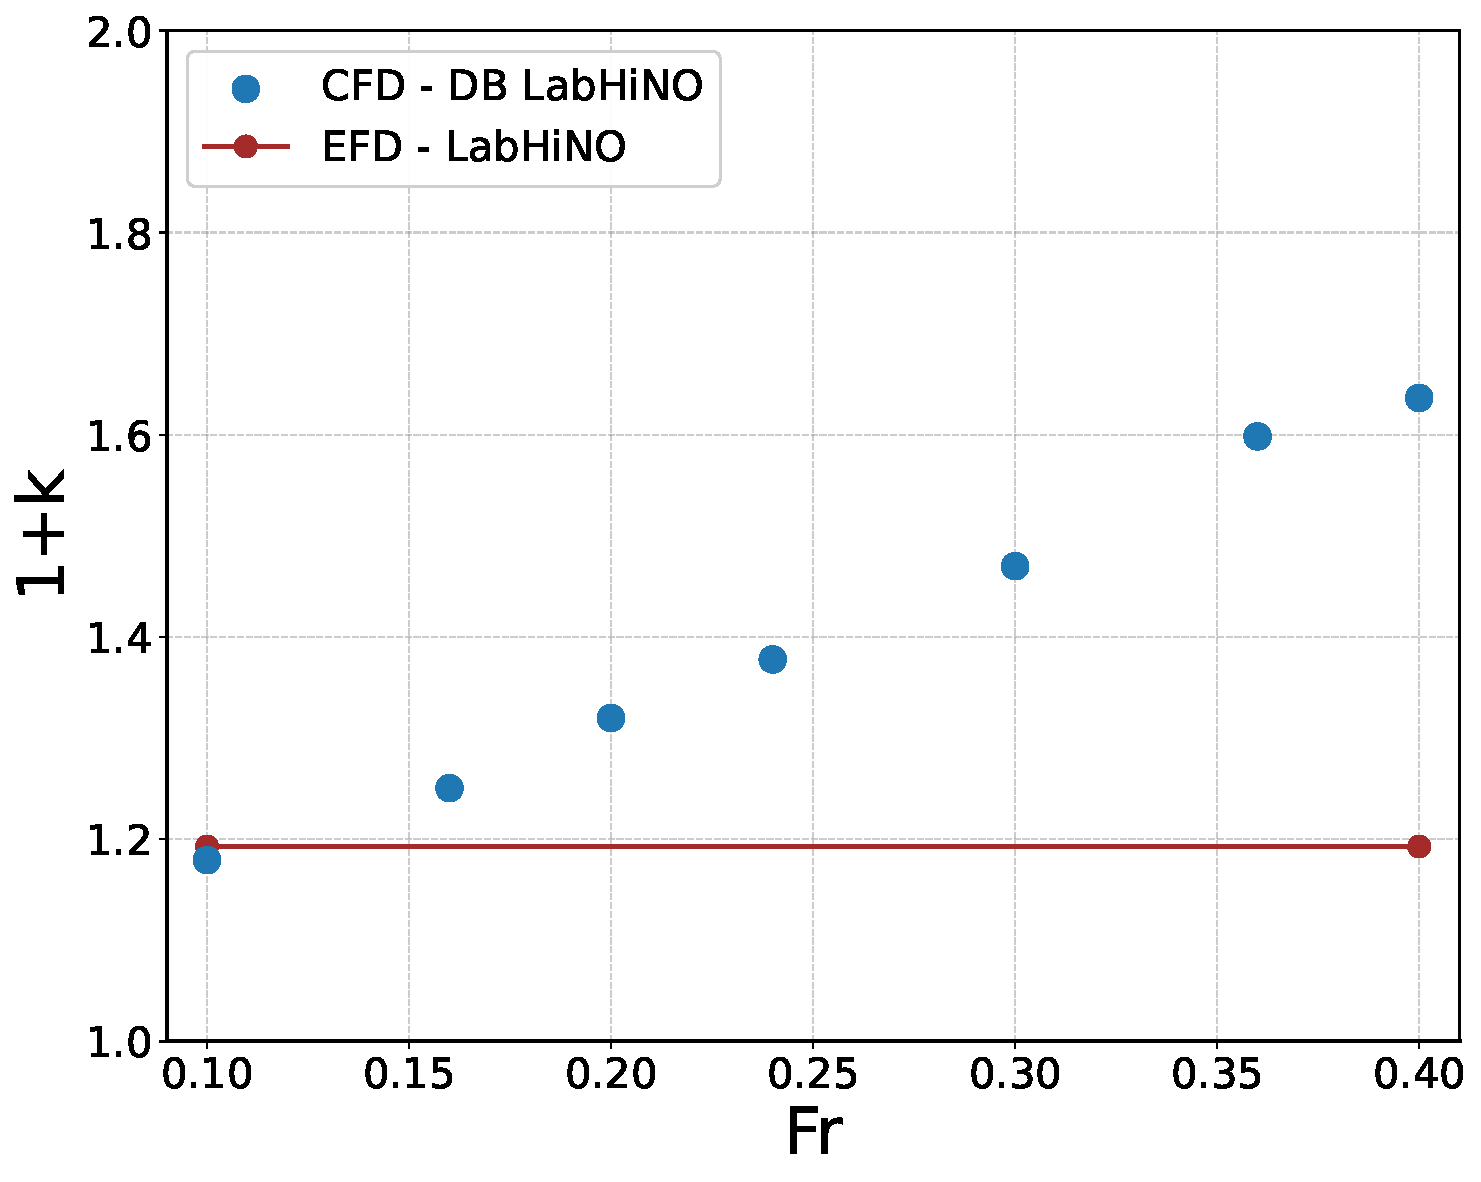
\includegraphics[width=\textwidth]{images/tpa_CFD_DB_prohaska_195.pdf}
         \caption{Calado 3.}
         \label{fig:tpa_proj_DB_k_escala20_195}
     \end{subfigure}
     
     \caption{Comparación del valor de $(1+k)$ adoptado por Prohaska (EFD/CFD, 
     línea roja) con la evolución de $(1+k)$ obtenida mediante el método de 
     doble cuerpo (puntos azules) en función de $Fr$, para los tres calados 
     del \textit{P1}.}
     \label{fig:comparativa_doble_cuerpo}
\end{figure}

\subsection{Discusión de incertidumbres y diferencias entre EFD y CFD}

Los resultados presentados hasta el momento permiten realizar una primera discusión conjunta sobre las incertidumbres involucradas y las diferencias observadas entre los ensayos experimentales (EFD) y las simulaciones numéricas (CFD) en la determinación de la resistencia al avance y del factor de forma $(1+k)$.

Desde el punto de vista experimental, la campaña realizada en el canal del LabHiNO mostró un nivel de repetibilidad adecuado y valores de incertidumbre combinada compatibles con las recomendaciones de la ITTC, especialmente en el rango de velocidades de interés operativo. Las curvas de resistencia obtenidas para los distintos calados presentan una evolución continua y físicamente consistente, lo que indica una correcta adquisición de la fuerza de remolque y una adecuada calibración del sistema de medición. No obstante, como es habitual en este tipo de ensayos, las mayores incertidumbres relativas se concentran en el rango de bajas velocidades, donde la resistencia total es pequeña y el método de Prohaska resulta particularmente sensible a pequeñas variaciones en $C_T$.

En este contexto, la aplicación del método de Prohaska a los datos experimentales evidenció desviaciones respecto de la linealidad teórica esperada, principalmente a bajos números de Froude. Tal comportamiento puede atribuirse a una combinación de factores: laminarización parcial del flujo, transición temprana, fenómenos viscosos locales asociados a la geometría del casco y limitaciones inherentes al uso de la línea de correlación ITTC-1957 en regímenes de Reynolds moderados. Estas desviaciones introducen una incertidumbre adicional en la estimación de $(1+k)$, que obliga a seleccionar cuidadosamente el rango de velocidades utilizado para la regresión lineal.

Las simulaciones CFD bifásicas reprodujeron de manera satisfactoria las curvas de resistencia total obtenidas experimentalmente en un amplio rango de velocidades, lo que constituye una primera validación global del modelo numérico. Las pequeñas diferencias observadas a velocidades elevadas pueden explicarse por diferencias en las condiciones de contorno dinámicas del casco, dado que en los ensayos experimentales se permitió el libre movimiento vertical y de cabeceo, mientras que en las simulaciones el casco se mantuvo fijo. En cualquier caso, estas discrepancias aparecen fuera del rango de operación típico del buque y no afectan las conclusiones principales.

En cuanto a la determinación del factor de forma mediante CFD, la aplicación directa del método de Prohaska mostró nuevamente desviaciones respecto de la recta teórica, aunque con una curvatura de signo opuesto a la observada experimentalmente. Esta diferencia pone de manifiesto una limitación conocida de los modelos RANS convencionales, que asumen flujo plenamente turbulento incluso en regímenes donde el flujo real se encuentra en transición. En consecuencia, tanto en EFD como en CFD, los puntos correspondientes a bajas velocidades no cumplen estrictamente los supuestos fundamentales del método de Prohaska, aunque por razones físicas y numéricas distintas.

La comparación sistemática entre EFD y CFD mostró que, al restringir el 
análisis a un rango adecuado de números de Froude, los valores de $(1+k)$ 
obtenidos por ambos enfoques mediante el método de Prohaska convergen de 
manera satisfactoria. Este resultado confirma que las discrepancias iniciales 
no responden a errores sistemáticos de medición o modelado, sino a la 
violación de los supuestos del método de Prohaska fuera de su rango óptimo de 
aplicación. La adopción de un intervalo reducido y físicamente consistente 
permitió reducir significativamente la dispersión y obtener valores 
comparables entre ambos enfoques.

Por último, la comparación entre el método de Prohaska (experimental y 
numérico) y el enfoque de doble cuerpo introdujo un nuevo elemento de análisis. 
Los valores de $(1+k)$ obtenidos mediante simulaciones de doble cuerpo, sin 
superficie libre, presentan una variación apreciable con la velocidad, lo que 
plantea interrogantes sobre la hipótesis de constancia del factor de forma 
asumida por el método de Prohaska. La superposición parcial entre los valores 
adoptados por Prohaska y el rango de resultados del método de doble cuerpo 
sugiere que ambos enfoques capturan distintos aspectos del mismo fenómeno 
viscoso, aunque con sensibilidades diferentes al régimen de flujo y al 
modelado de la turbulencia.

En síntesis, los resultados obtenidos hasta acá indican que:
\begin{itemize}
    \item Las mediciones experimentales presentan niveles de incertidumbre 
    compatibles con estándares internacionales y constituyen una base 
    confiable para la validación numérica.
    \item El método de Prohaska es altamente sensible a las condiciones de 
    flujo a bajas velocidades, tanto en EFD como en CFD, lo que exige una 
    selección cuidadosa del rango de aplicación.
    \item Las simulaciones CFD con superficie libre reproducen adecuadamente 
    la resistencia total, pero introducen limitaciones adicionales en 
    regímenes transicionales debido a las hipótesis del modelo de turbulencia.
    \item La concordancia entre EFD y CFD mejora significativamente cuando se 
    restringe el análisis a rangos donde los supuestos físicos del método de 
    Prohaska son razonablemente válidos.
\end{itemize}

Estas observaciones establecen un marco sólido para los análisis posteriores, 
donde se profundizará en la descomposición de la resistencia viscosa y en la 
interpretación física de las variaciones de $(1+k)$ con la velocidad 
observadas mediante el método de doble cuerpo.

\subsection{Análisis de efectos de escala} \label{sec:analisis_efectos_escala}

\paragraph{Extensión de escalas}

Con el fin de resaltar el comportamiento distintivo de $(1+k)$ en función de 
$Re$ que se ha encontrado para el \textit{P1}, en esta subsección se compara 
dicho comportamiento con el correspondiente al KCS. A diferencia de las 
secciones anteriores, donde $(1+k)$ se presentó en función de $Fr$ para un 
único buque a una escala fija, aquí se opta por graficar en función de $Re$, 
dado que esta variable permite comparar directamente resultados provenientes 
de buques y escalas distintas (KCS a 1:79 y 1:75, y \textit{P1} a 1:20) en un 
mismo eje, algo que $Fr$ no posibilita al depender únicamente de la velocidad 
relativa a la eslora de cada modelo.

En primer lugar, con el propósito de una mayor claridad analítica, los 
resultados presentados en las Figuras~\ref{fig:k_195} y \ref{fig:kcs_DB_prohaska} 
se reúnen en la Figura~\ref{fig:comparacion_total_kcs_tpa}.

La Figura~\ref{fig:comparacion_total_kcs_tpa} muestra los valores de $(1+k)$ 
frente a $Re$ obtenidos mediante CFD \textit{double body} (DB) para el KCS 
a escala 1:79, el KCS a escala 1:75 de \citet{TERZIEV2021147} y el \textit{P1} 
en escala modelo (1:20) para el Calado~3. El gráfico incluye además los 
valores experimentales (EFD) de $(1+k)$ determinados mediante el método de 
Prohaska en el presente trabajo, para el KCS a escala 1:79 y para el 
\textit{P1}.

\begin{figure}[htpb]
	\centering
	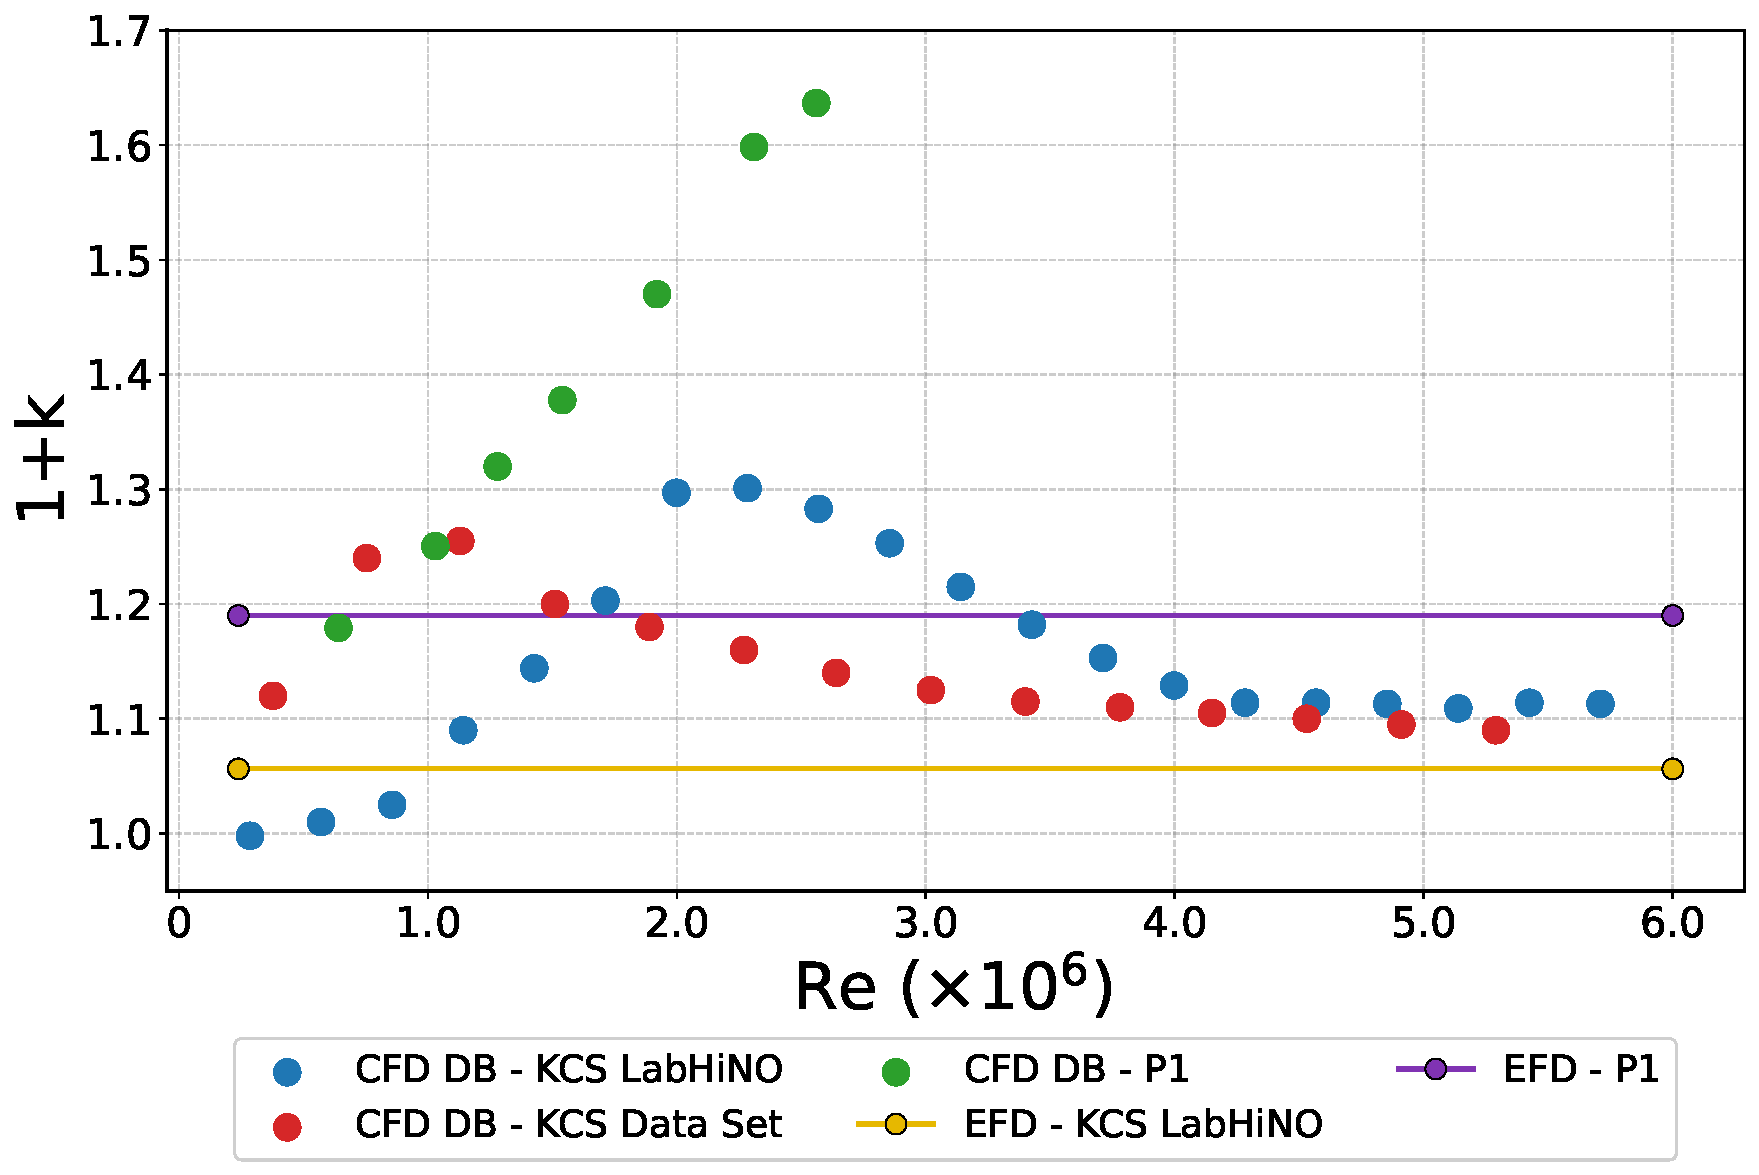
\includegraphics[width=.6\columnwidth]{images/comparacion_total_kcs_tpa.pdf}
	\caption{$(1+k)$ frente a $Re$ para el KCS (CFD DB, escalas 1:79 y 1:75 
	de \citet{TERZIEV2021147}, y EFD a 1:79) y para el \textit{P1} (CFD DB y 
	EFD, escala 1:20, Calado~3).}
	\label{fig:comparacion_total_kcs_tpa}
\end{figure}

Es evidente que, dentro del rango de velocidades del modelo considerado, el 
\textit{P1} no alcanza un valor asintótico de $(1+k)$, a diferencia de lo 
observado en el KCS. Por consiguiente, y en contraste con el comportamiento 
mostrado por el KCS, el valor de $(1+k)$ del \textit{P1} calculado mediante 
CFD DB se desvía progresivamente del valor obtenido por el método de 
Prohaska, ya sea numérica o experimentalmente, a medida que aumenta la 
velocidad del modelo.

Para comprender mejor el comportamiento de $(1+k)$ en función de $Re$ en el 
caso del \textit{P1}, se realizaron cálculos CFD DB de $(1+k)$ para diferentes 
escalas de modelo, con el fin de abarcar un rango más amplio de $Re$. Se 
evaluaron la escala 1:20 (ya presentada) y tres escalas adicionales, 1:10, 
1:5 y 1:1.

\begin{figure}[htpb]
	\centering
	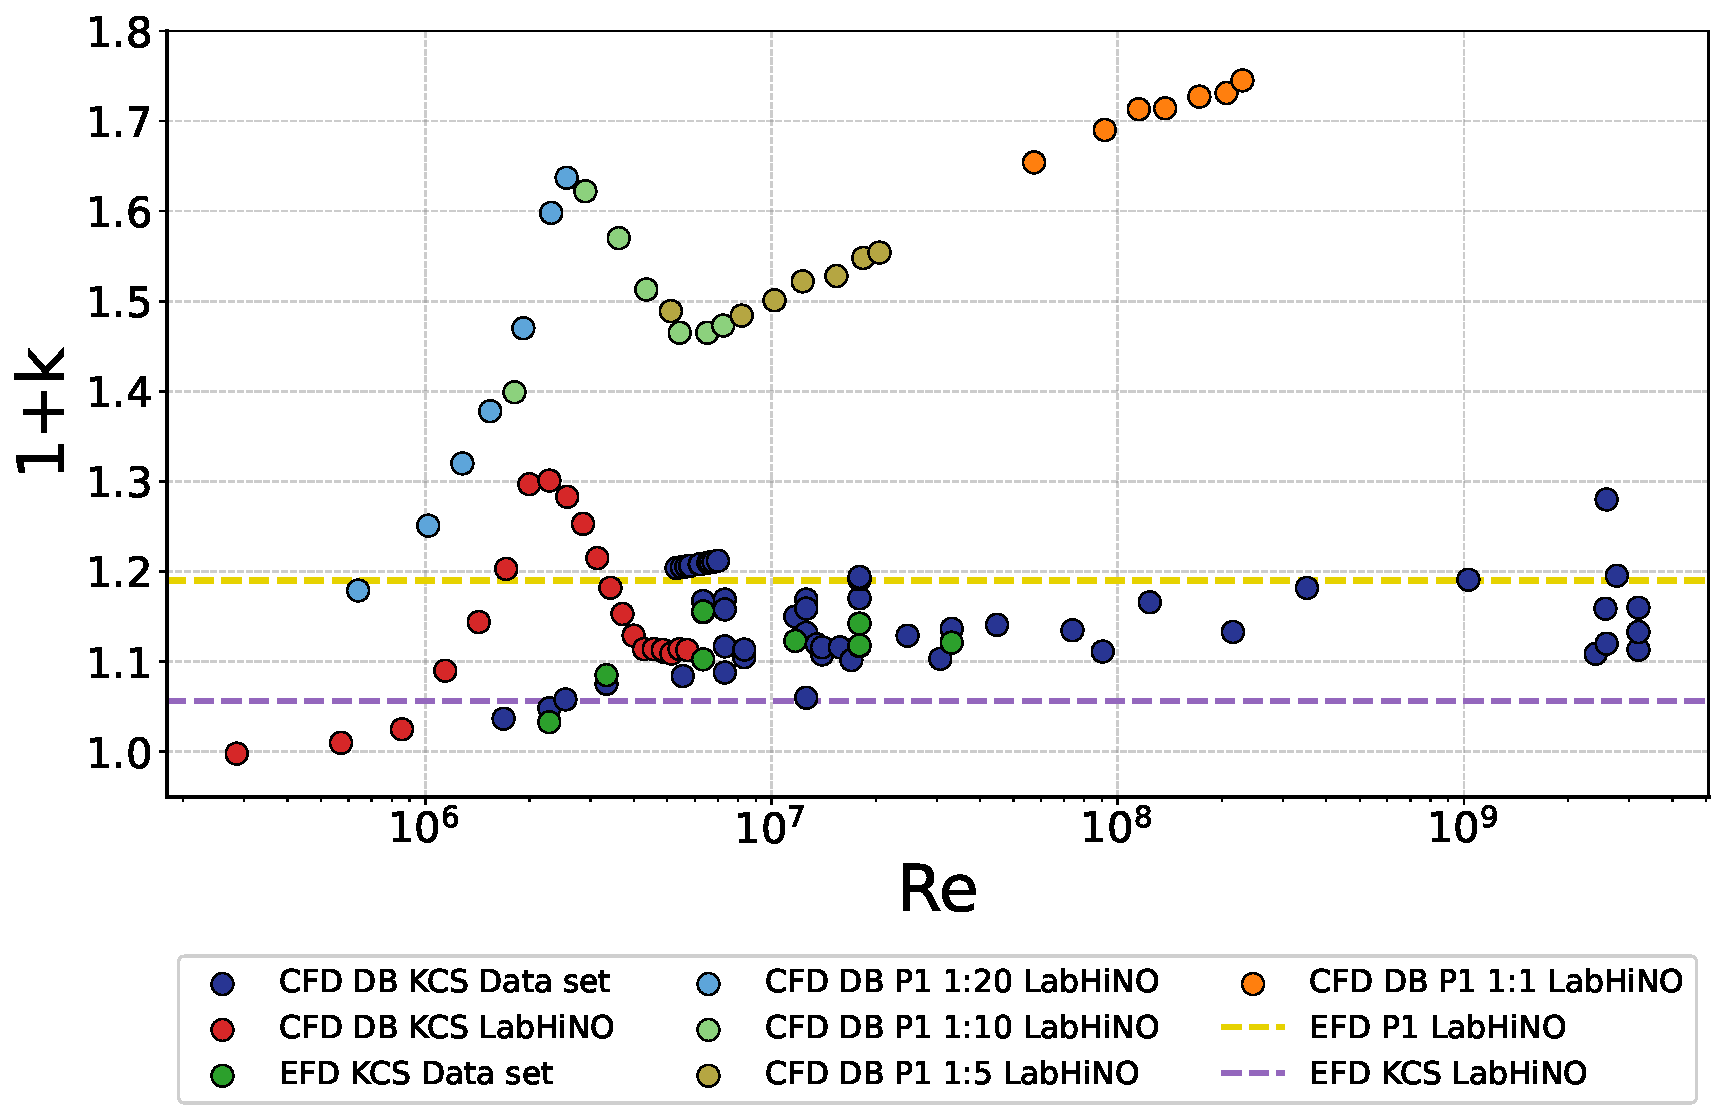
\includegraphics[width=.6\columnwidth]{images/completo_log_kcs_lit_tpa.pdf}
	\caption{$(1+k)$ frente a $Re$ para el KCS y el \textit{P1}, en escala 
	logarítmica. Para el KCS se muestran los resultados propios obtenidos en 
	el LabHiNO (CFD DB y Prohaska EFD, escala 1:79) junto con el conjunto de 
	datos recopilado por \citet{TerzievDataSet} (CFD DB y Prohaska, otras 
	escalas y laboratorios). Para el \textit{P1} se muestran únicamente 
	resultados propios: CFD DB en las escalas 1:20, 1:10, 1:5 y 1:1, y el 
	valor experimental obtenido por Prohaska en el LabHiNO (escala 1:20).}
	\label{fig:comparacion_total_escalas_kcs_tpa}
\end{figure}

La Figura~\ref{fig:comparacion_total_escalas_kcs_tpa} permite contextualizar 
los resultados del \textit{P1} dentro de la tendencia general documentada para 
el KCS en la literatura, y extender el análisis del \textit{P1} a un rango 
más amplio de $Re$ mediante simulaciones a distintas escalas geométricas.

Se observa que el modelo CFD DB presenta, para ambos buques estudiados, un 
pico aproximadamente en el mismo rango de $Re$. Como se mencionó previamente, 
este pico podría estar directamente asociado con la modelización de la 
transición.

Por otro lado, se observa en la Figura que la variación de $(1+k)$ con $Re$ 
disminuye para el KCS a valores altos de $Re$, mientras que para el 
\textit{P1} la tendencia creciente persiste hasta la escala buque (1:1), sin 
alcanzar un valor asintótico dentro del rango analizado.

El impacto de $Re$ sobre el valor de $(1+k)$ es considerablemente más 
pronunciado en el \textit{P1}. A modo ilustrativo, la diferencia entre el 
valor de $(1+k)$ a bajo $Re$ y a alto $Re$ es aproximadamente del 40\% para 
el \textit{P1}, mientras que para el KCS es cercana al 8\%. Además, el valor 
final de $(1+k)$ del \textit{P1} resulta casi un 50\% superior al del KCS, 
valor no encontrado en la literatura de hidrodinámica naval al día de hoy.

Para verificar que este comportamiento no es exclusivo del \textit{P1}, 
se extendió el análisis CFD DB a los otros dos pesqueros analizados en 
esta tesis (\textit{P2}, $L/B = 3{.}23$; \textit{P3}, $L/B = 2{.}85$). 
La Figura~\ref{fig:Re_formfactor} muestra la evolución de $(1+k)$ con 
$Re$ para los cuatro cascos. Los tres pesqueros presentan el mismo 
comportamiento creciente y no asintótico observado en el \textit{P1}, en 
marcado contraste con la estabilización del KCS. Esta consistencia 
confirma que la falta de valor asintótico de $(1+k)$ no es una 
singularidad del \textit{P1}, sino una característica común a los 
pesqueros estudiados. Las causas geométricas de este comportamiento se 
analizan en profundidad en la Sección~\ref{sec:generalizacion_LB}.

\begin{figure}[htpb]
    \centering
    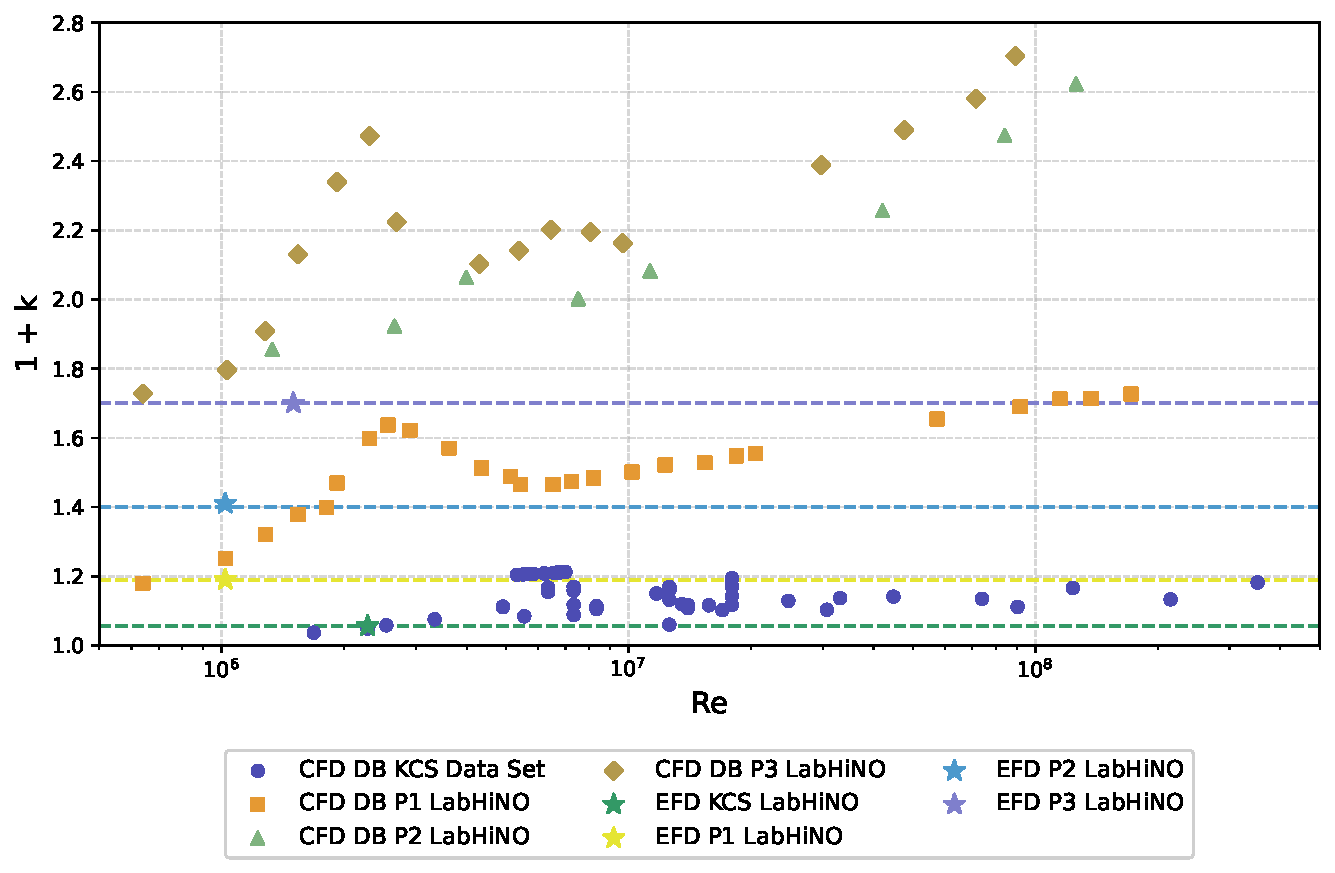
\includegraphics[width=.6\textwidth]{./images/completo_log_kcs_lit_tpa_jpa_contessi.pdf}
    \caption{Evolución de $(1+k)$ con el número de Reynolds para el KCS 
    y los tres pesqueros analizados.}
    \label{fig:Re_formfactor}
\end{figure}

El método de \citet{gomezgarcia} (Sección~\ref{sec:factor_de_forma_antec})
ofrece una prueba cuantitativa directa de cuán anómalo resulta el
comportamiento del \textit{P1}. Aplicando su relación empírica
[Ecuación~\eqref{eq:gomezgarcia}] a la escala del modelo ($\lambda = 20$), el efecto de escala predicho es $K_S - K_M \approx 1{.}91\times 19\times 10^{-3}= 0{.}036$. El valor obtenido por CFD de doble cuerpo para el \textit{P1} en el Calado~3, en cambio, es $k_S - k_M = 0{.}716 - 0{.}194 = 0{.}522$, es decir, aproximadamente catorce veces mayor que la predicción. La fórmula de \citet{gomezgarcia}, calibrada para estimar la corrección de escala del factor de forma, subestima en más de un orden de magnitud el efecto de escala real de este casco.

Esta discrepancia no se limita a la magnitud, sino que alcanza a la propia
forma funcional. Al ajustar el modelo lineal de \citet{gomezgarcia} —$K_S -
K_M$ en función de $\lambda$— a los cuatro puntos de escala calculados para el \textit{P1} (1:20, 1:10, 1:5 y 1:1), la pendiente resultante es de
$15{.}8\times 10^{-3}$, más de ocho veces la de $1{.}851\times 10^{-3}$ de la regresión original (Figura~\ref{fig:gomez-garcia-nuestro}). Más significativo aún es que el ajuste lineal del \textit{P1} arroja una ordenada al origen de $0{.}054$, de modo que predice un efecto de escala espurio de $K_S - K_M \approx 0{.}070$ en $\lambda = 1$, condición en la que necesariamente debe anularse. La regresión de \citet{gomezgarcia}, en cambio, satisface esta restricción física ($K_S - K_M \approx 0{.}001$ en $\lambda = 1$). El modelo lineal, por lo tanto, no puede recuperarse reescalando la pendiente: la hipótesis de linealidad en $\lambda$ sobre la que se apoya no se cumple para esta clase de casco.

El origen de esta inaplicabilidad es geométrico. Las cuatro familias de
geosims sobre las que \citet{gomezgarcia} calibró su correlación corresponden a cascos esbeltos convencionales, con relaciones $L_{PP}/B$ comprendidas entre $6{.}98$ y $9{.}07$; ninguna se aproxima siquiera a la baja esbeltez del \textit{P1} ($L/B \approx 2{.}8$--$3{.}5$). La correlación se aplica, por lo tanto, fuera del dominio para el que fue derivada, en un régimen donde la resistencia por presión viscosa, despreciable en los cascos esbeltos de lamuestra original, pasa a ser una fracción dominante de la resistencia viscosa total, como se demuestra en la
Sección~\ref{sec:descomposicion_de_la_res_viscosa}.

\begin{figure}[htpb]
\centering
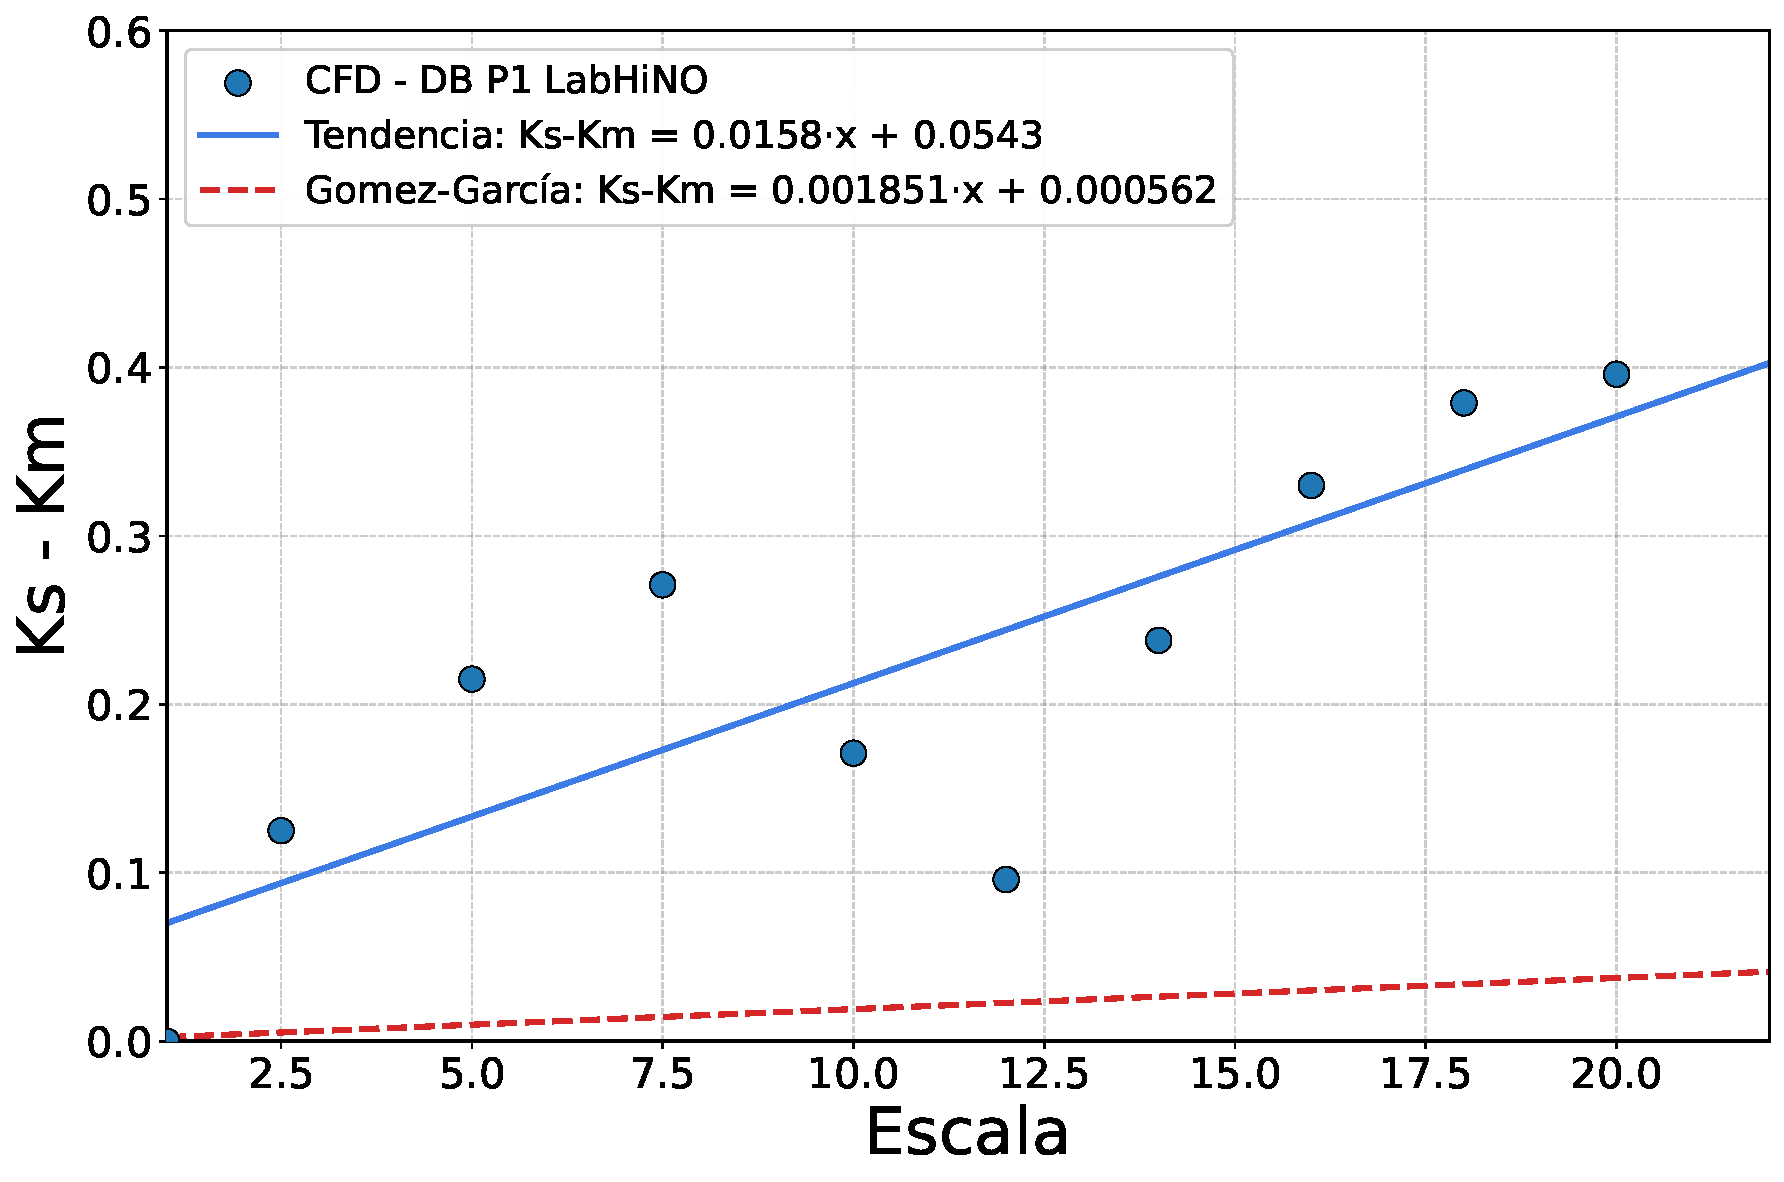
\includegraphics[width=0.6\textwidth]{images/gomez-garcia-nuestro.pdf}
\caption{Efecto de escala del factor de forma del \textit{P1}, $k_S - k_M$,
en función de la razón de escala $\lambda$, con la recta de regresión lineal ajustada a los puntos calculados por CFD de doble cuerpo. Se incluye, para comparación, la recta de \citet{gomezgarcia}.}
\label{fig:gomez-garcia-nuestro}
\end{figure}

De manera similar, el método de \citet{keh-sik-min} (Sección~\ref{sec:factor_de_forma_antec}) 
podría ser aplicado exitosamente al KCS, dado que se observa dicho factor de 
forma terminal a altos valores de $Re$, pero no así al \textit{P1}, donde 
$(1+k)$ no alcanza un valor asintótico dentro del rango analizado. Esto 
motiva la siguiente sección, donde se analizan las posibles razones de este 
aumento continuo del factor de forma.


\subsection{Descomposición de la resistencia viscosa} \label{sec:descomposicion_de_la_res_viscosa}

A diferencia del ensayo experimental, donde solo es posible medir la fuerza 
total de resistencia, la simulación CFD en configuración de doble cuerpo 
permite separar explícitamente las contribuciones friccional y de presión 
viscosa, lo que posibilita el análisis detallado que se presenta en esta 
sección. Esta descomposición se basa en la relación:
%
\begin{equation}
    (1+k) = \frac{C_V}{C_{F0}} = \frac{C_F + C_{PV}}{C_{F0}}
    \label{eq:descomposicion_1k}
\end{equation}
%
donde $C_F$ es el coeficiente de resistencia friccional, $C_{PV}$ el 
coeficiente de resistencia por presión viscosa y $C_{F0}$ el coeficiente de 
la línea de correlación ITTC-57. La Ecuación~\eqref{eq:descomposicion_1k} 
permite anticipar el comportamiento de $(1+k)$ con $Re$: si $C_{PV}$ 
disminuye con $Re$ más lentamente que $C_{F0}$ en el denominador, el 
cociente continúa creciendo aun cuando ambos coeficientes decaigan en 
términos absolutos.

La Figura~\ref{descomposicion_fuerzas} muestra el coeficiente de resistencia 
total ($C_T$), el coeficiente de resistencia friccional ($C_F$) y el 
coeficiente de resistencia por presión viscosa ($C_{PV}$) obtenidos a partir 
de la simulación CFD en configuración de doble cuerpo (DB) para el 
\textit{P1}, en función del número de Reynolds ($Re$). Asimismo, se incluye 
la línea de correlación ITTC-57 ($C_{F0}$) a efectos comparativos.

\begin{figure}
\centering
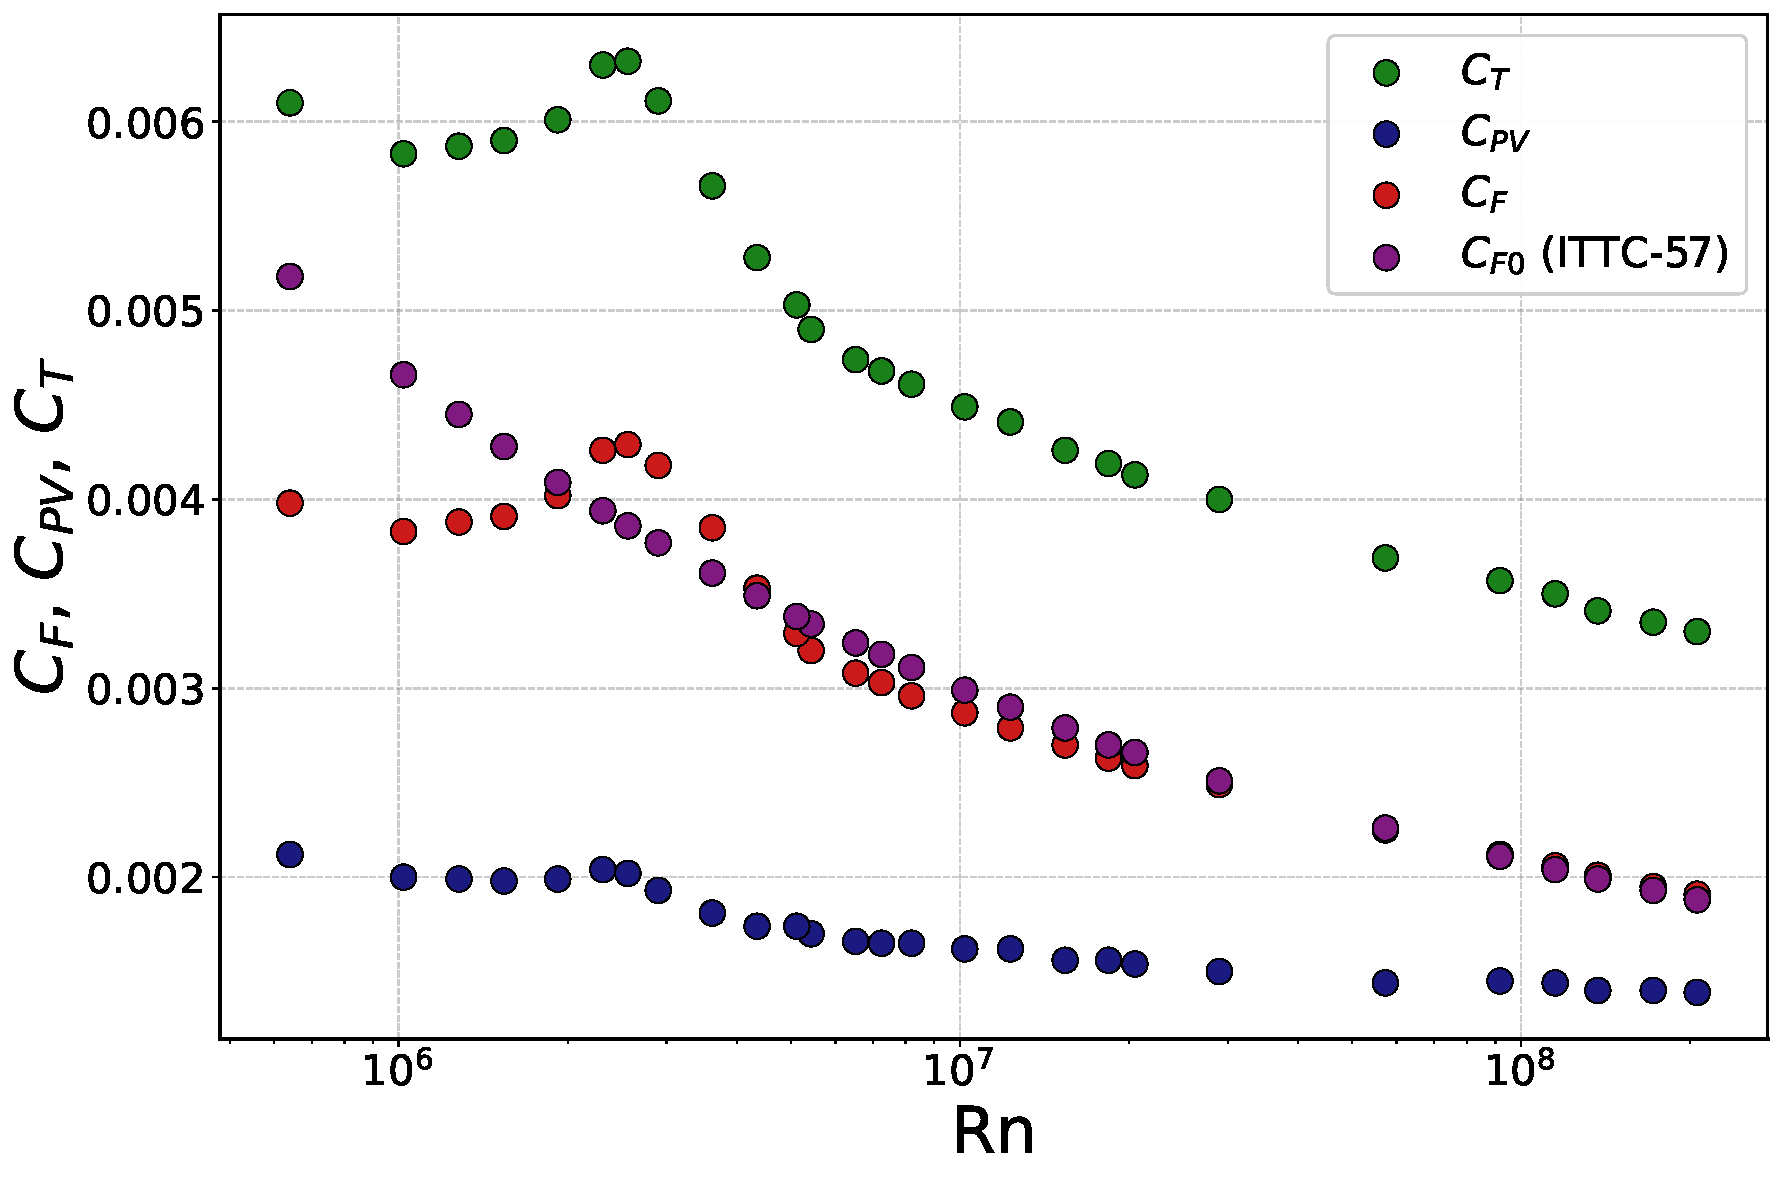
\includegraphics[width=.6\columnwidth]{./images/descomposicion_coeficientes.pdf}
\caption{Coeficientes $C_T$, $C_{PV}$ y $C_F$ obtenidos mediante CFD en 
configuración de doble cuerpo, junto con la línea ITTC-57 ($C_{F0}$), en 
función de $Re$ para el \textit{P1}.}
\label{descomposicion_fuerzas}
\end{figure}

El coeficiente de resistencia friccional ($C_F$) del modelo CFD-DB coincide 
estrechamente con la correlación ITTC-57 para valores de $Re$ mayores que 
$5\times 10^6$, es decir, más allá de la región de transición. En cambio, 
$C_{PV}$ disminuye de manera muy lenta con $Re$. Según la 
Ecuación~\eqref{eq:descomposicion_1k}, esta disminución lenta de $C_{PV}$ en 
el numerador, combinada con la disminución más rápida de $C_{F0}$ en el 
denominador, genera el incremento sostenido de $(1+k)$ observado. La tasa de 
crecimiento de $(1+k)$ con $Re$ disminuye a medida que aumenta $Re$, 
fundamentalmente debido a la meseta que alcanza $C_F$.

Para analizar el comportamiento característico de $C_{PV}$, la 
Figura~\ref{cpv_friccion} compara los valores de $C_F$ y $C_{PV}$ obtenidos 
para el \textit{P1} y para el KCS. Se observa que, en todo el rango de 
Reynolds considerado, el valor de $C_{PV}$ del \textit{P1} es sustancialmente 
superior al del KCS, y que dicha diferencia se mantiene prácticamente sin 
disminuir a medida que aumenta $Re$. Cualitativamente, mientras que en el 
KCS $C_F$ domina ampliamente sobre $C_{PV}$ en todo el rango analizado, en el 
\textit{P1} ambos coeficientes resultan de magnitud comparable, lo que indica 
que la presión viscosa constituye una fracción mucho más significativa de la 
resistencia viscosa total para este casco.

\begin{figure}
\centering
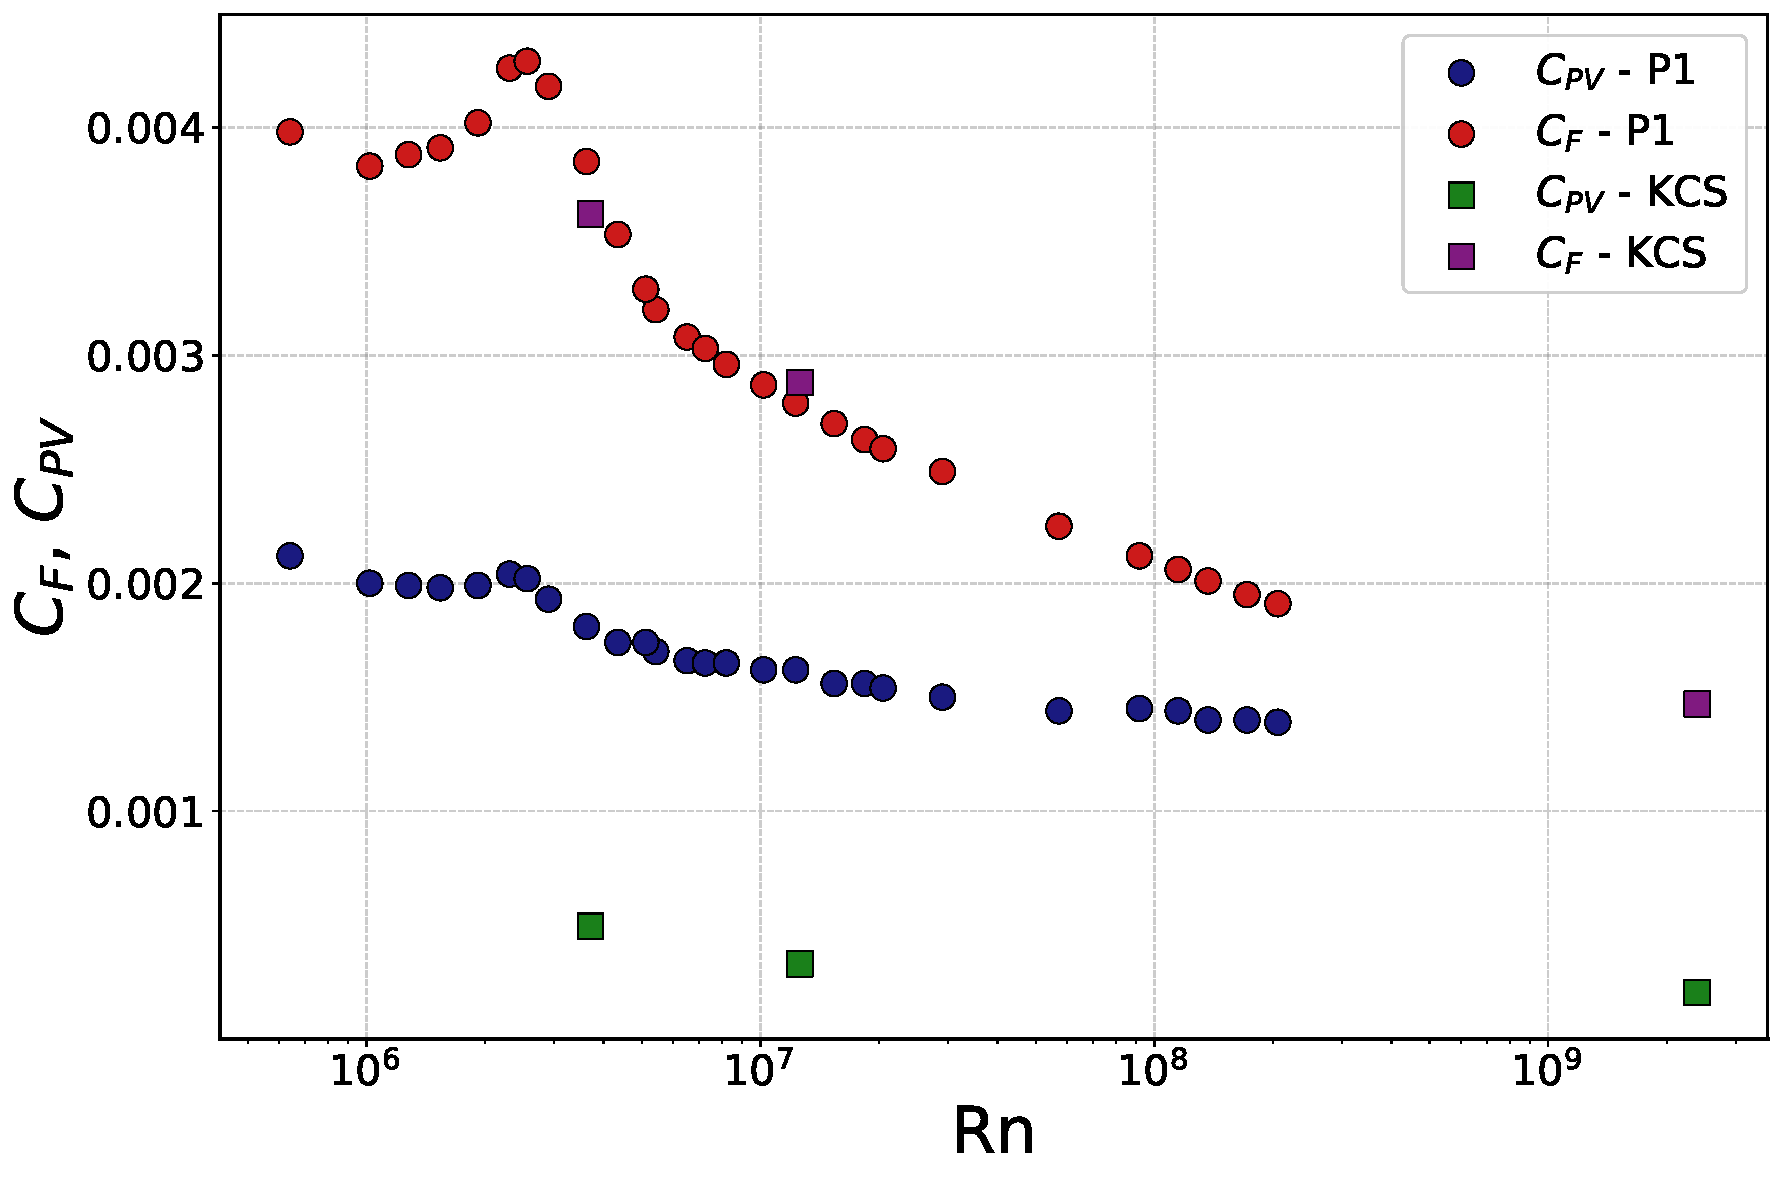
\includegraphics[width=.6\columnwidth]{./images/kcs_tpa_descomposicion.pdf}
\caption{$C_{PV}$ y $C_F$ obtenidos mediante CFD en doble cuerpo para el 
\textit{P1} y para el KCS 1:79 (LabHiNO).}
\label{cpv_friccion}
\end{figure}

A diferencia de $C_F$, el coeficiente $C_{PV}$ es poco sensible a variaciones 
de $Re$ y resulta fuertemente influenciado por la geometría del casco. Para 
comprender esta dependencia con la forma del casco, es necesario considerar 
dos mecanismos que compiten en la formación de la resistencia por presión 
viscosa. El primero es la contribución de la capa límite tridimensional, que 
disminuye con $Re$ a medida que la capa límite se adelgaza y se reduce la 
disipación de energía cinética viscosa a lo largo del casco. El segundo es la 
contribución de estructuras vorticosas generadas en el casco, entre las que 
se incluyen tanto vórtices longitudinales desprendidos de la quilla y el 
pantoque como la posible recirculación asociada a la popa espejo, cuya 
intensidad puede aumentar o mantenerse aproximadamente estable con $Re$. La 
curva resultante de $C_{PV}(Re)$ surge de la superposición de estas dos 
tendencias opuestas (capa límite vs. estructuras vorticosas). 
Interpretaciones similares de doble mecanismo han sido reportadas por 
\citet{ZENG2019106434} y \citet{Raven2016}, y son consistentes con los 
estudios de escalado de popas mojadas de \citet{KORKMAZ2022112590}. El aporte 
relativo de cada una de estas fuentes de vorticidad se analiza en detalle en 
la Sección~\ref{sec:popa_sumergida}.

La Figura~\ref{U_x_U_0} presenta contornos de la velocidad longitudinal 
$U_x/U_0$ a $x/L=0.05$, inmediatamente detrás de la sección de popa, para 
escala modelo (1:20, $Re \approx 10^6$) y escala buque (1:1, $Re \approx 10^8$), donde se aprecia el adelgazamiento de la capa límite con $Re$, como cabría esperar del primer mecanismo. Por otro lado, la Figura~\ref{vortex} muestra iso-superficies de criterio Q que revelan el sistema de estructuras 
vorticosas presentes en la popa para ambas escalas. Dichas estructuras se 
mantienen con intensidad similar al aumentar $Re$, lo que indica que es la 
persistencia de este segundo mecanismo, y no el primero, la causa del alto 
valor de $C_{PV}$ y de su débil sensibilidad al número de Reynolds para el 
\textit{P1}. La pequeña disminución de $C_{PV}$ con $Re$ observada puede 
atribuirse al efecto superpuesto de la reducción de la capa límite.

\begin{figure}
\centering
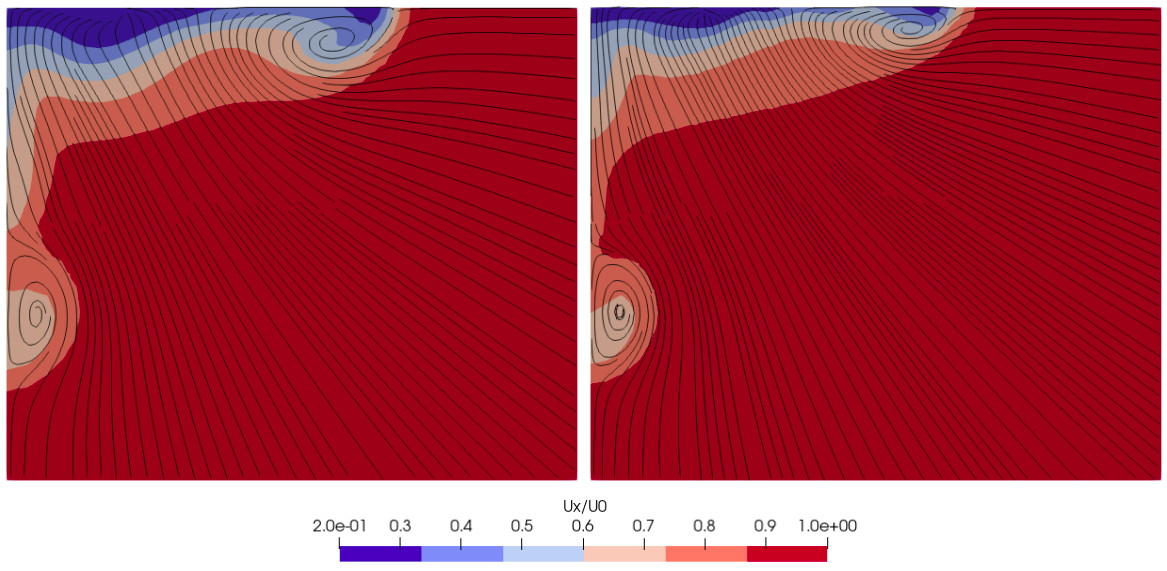
\includegraphics[width=1\columnwidth]{./images/U_x_U_0.png}
\caption{Contornos de velocidad longitudinal $U_x/U_0$ en un plano ubicado en 
$x/L=0.05$ para escala modelo, 1:20 (izquierda, $\log(Re) \approx 6$) y 
escala buque, 1:1 (derecha, $\log(Re) \approx 8$), a $Fr=0.2$.}
\label{U_x_U_0}
\end{figure}

\begin{figure}
\centering
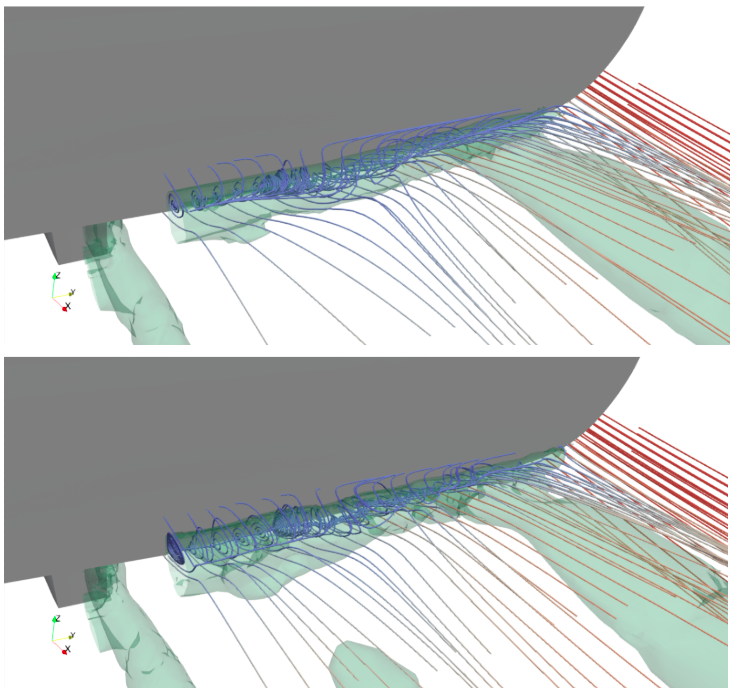
\includegraphics[width=.8\columnwidth]{./images/vortex.png}
\caption{Iso-superficies de Q-criterion (Q=10) mostrando las estructuras 
vorticosas presentes en la popa, a escala modelo, 1:20 (arriba, 
$\log(Re) \approx 6$) y escala buque, 1:1 (abajo, $\log(Re) \approx 8$), 
a $Fr=0.2$.}
\label{vortex}
\end{figure}

En síntesis, la descomposición presentada en esta sección permite explicar el 
comportamiento contrastante de $(1+k)$ entre ambos buques observado en la 
Sección~\ref{sec:analisis_efectos_escala}. En el KCS, la contribución de 
$C_{PV}$ al numerador de la Ecuación~\eqref{eq:descomposicion_1k} es 
comparativamente pequeña frente a $C_F$, de modo que $(1+k)$ queda dominado 
por el comportamiento de $C_F$, que sigue de cerca a $C_{F0}$ más allá de la 
región de transición y produce así un cociente prácticamente constante. En 
el \textit{P1}, en cambio, la magnitud comparable y la lenta caída de 
$C_{PV}$ frente a la caída más rápida de $C_{F0}$ impiden que el cociente se 
estabilice dentro del rango de escalas analizado. Este mecanismo, sostenido 
por la persistencia de estructuras vorticosas en la popa que no se atenúan 
significativamente con $Re$, es el responsable directo de la falta de valor 
asintótico de $(1+k)$ característica de este casco.

\subsubsection*{Taxonomía de mecanismos de efecto de escala}

Los resultados presentados permiten ubicar el comportamiento del
\textit{P1} dentro de un panorama más amplio de mecanismos por los cuales
el factor de forma puede depender de la escala. La literatura documenta al
menos tres mecanismos distintos, que se diferencian tanto por su origen
físico como por el signo de su efecto sobre $(1+k)$ al aumentar el número
de Reynolds.

El primero es la \textbf{separación tipo burbuja} en la popa de cascos de
formas llenas, originada por el gradiente de presión adverso que sigue a la
región de baja presión del pantoque. A medida que aumenta $Re$, la
influencia de la viscosidad disminuye, la separación se atenúa y la
contribución de la resistencia de forma respecto de la viscosa se reduce,
de modo que $(1+k)$ \textit{decrece} con la escala
\citep{korkmaz-verif-and-valid-cfd-efd}. El segundo es la
\textbf{recirculación tras un espejo de popa sustancialmente sumergido},
análoga al flujo sobre un escalón hacia atrás. A diferencia del anterior,
esta estructura persiste al aumentar $Re$ y genera un incremento acotado
del factor de forma entre modelo y buque, cuantificado mediante el
\textit{transom form factor} $k_{tr}>0$ \citep{korkmaz_wetted_transom}; su
aplicación al \textit{P1} se analiza en la
Sección~\ref{sec:popa_sumergida}.

El mecanismo dominante en el \textit{P1}, en cambio, es distinto de ambos y
responde a la geometría de baja esbeltez del casco: se trata de la
persistencia de \textbf{estructuras vorticosas longitudinales} desprendidas
de la quilla y el pantoque, cuya intensidad no se atenúa apreciablemente
con $Re$, según se documentó mediante los contornos de velocidad
(Figura~\ref{U_x_U_0}) y las iso-superficies de criterio Q
(Figura~\ref{vortex}). Este mecanismo sostiene un valor elevado y poco
sensible de $C_{PV}$, lo que hace que $(1+k)$ \textit{crezca} de manera
sostenida y sin alcanzar un valor asintótico dentro del rango de escalas
analizado. El contraste de signo respecto de la separación tipo burbuja es
significativo: mientras en aquel caso el aumento de $Re$ tiende a
\textit{recuperar} el comportamiento de placa plana, en los pesqueros de
baja esbeltez el efecto tridimensional persiste hasta la escala buque. Esta
diferencia es la que confiere carácter distintivo al resultado y la que
explica por qué las correcciones concebidas para los dos primeros
mecanismos resultan insuficientes para esta clase de cascos, como se
verifica en las Secciones~\ref{sec:popa_sumergida}
y~\ref{sec:linea_de_friccion}.

\subsection{Distribución de presiones sobre el casco}

En esta sección se analiza la distribución del coeficiente de presión 
($C_P$) sobre el casco del \textit{P1} para distintas escalas. Este 
parámetro se define como:

\begin{equation}
    C_{P} = \frac{p - p_\infty}{\tfrac{1}{2}\rho V^2},
\end{equation}

donde $p$ es la presión sobre el casco, $p_\infty$ la presión del flujo 
incidente sin perturbaciones, $V$ la velocidad del buque y $\rho$ la densidad 
del agua. El coeficiente $C_{PV}$ surge de integrar $C_P$ sobre la superficie 
mojada y proyectarlo en la dirección de avance, por lo que el estudio 
detallado de su distribución permite comprender mejor la evolución de 
$C_{PV}$ con el número de Reynolds.

Las Figuras~\ref{cp_bow}, \ref{cp_stern}, \ref{cp_bottom} y \ref{cp_side} 
muestran la distribución de $C_P$ sobre el casco del \textit{P1} para escala 
modelo (1:20) y escala buque (1:1), a $Fr=0.2$, vistas desde la proa, la 
popa, el fondo y el costado respectivamente.

\begin{figure}
\centering
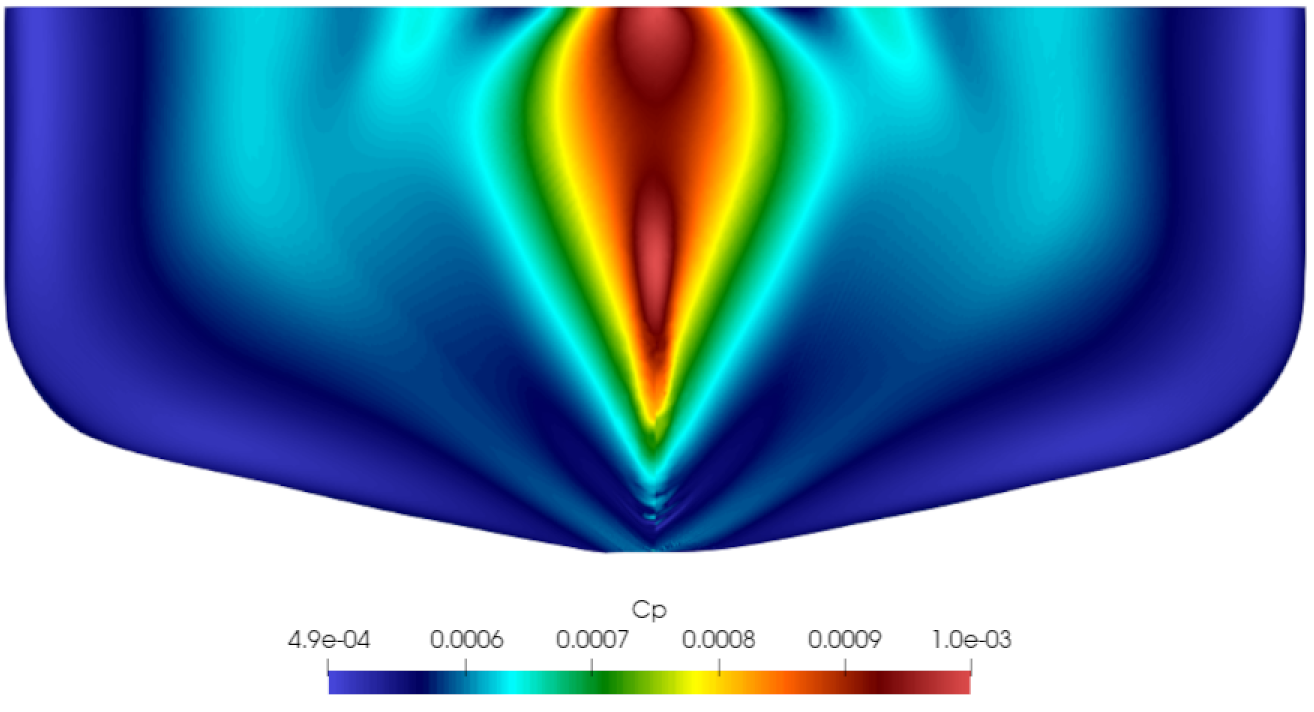
\includegraphics[width=.6\columnwidth]{./images/cp_proa2.png}
\caption{$C_P$ para $Fr=0.2$, vista de proa. Izquierda: escala 1:20. 
Derecha: escala 1:1.}
\label{cp_bow}
\end{figure}

\begin{figure}
\centering
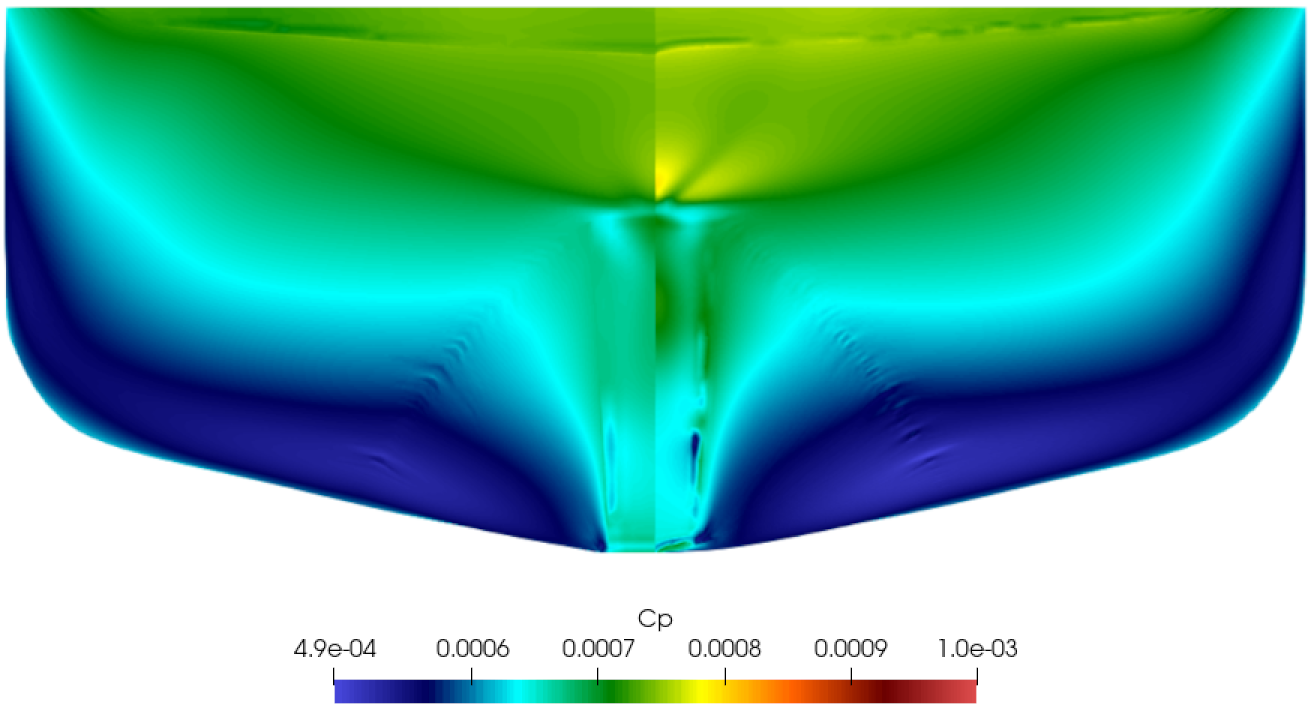
\includegraphics[width=.6\columnwidth]{./images/cp_popa2.png}
\caption{$C_P$ para $Fr=0.2$, vista de popa. Izquierda: escala 1:20. 
Derecha: escala 1:1.}
\label{cp_stern}
\end{figure}

\begin{figure}
\centering
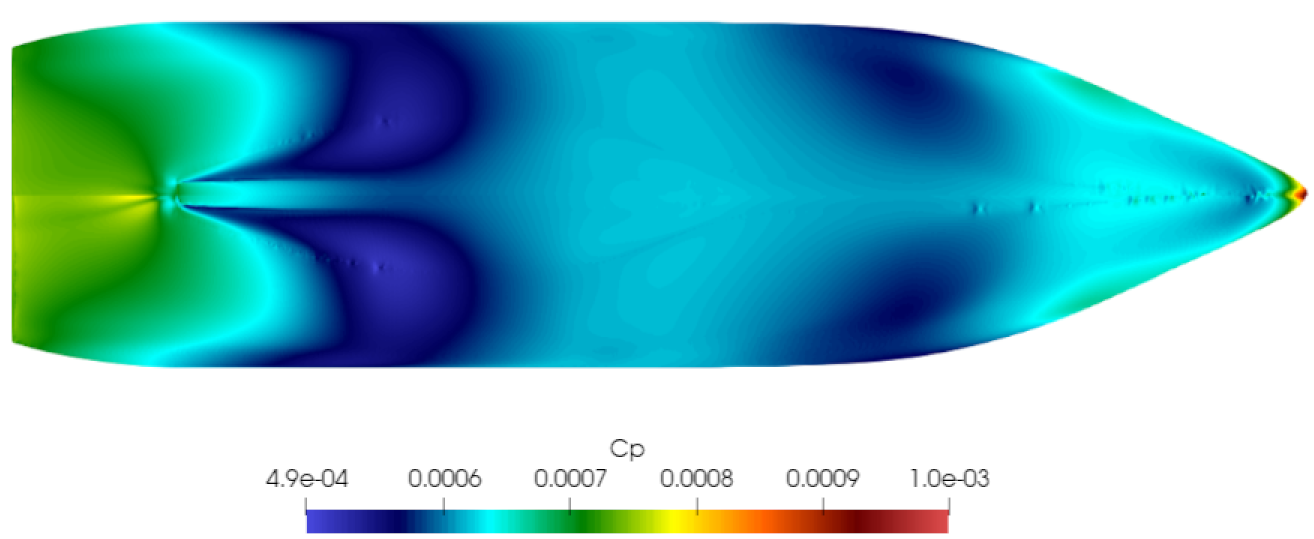
\includegraphics[width=.6\columnwidth]{./images/cp_fondo2.png}
\caption{$C_P$ para $Fr=0.2$, vista desde el fondo. Arriba: escala 1:20. 
Abajo: escala 1:1.}
\label{cp_bottom}
\end{figure}

\begin{figure}
\centering
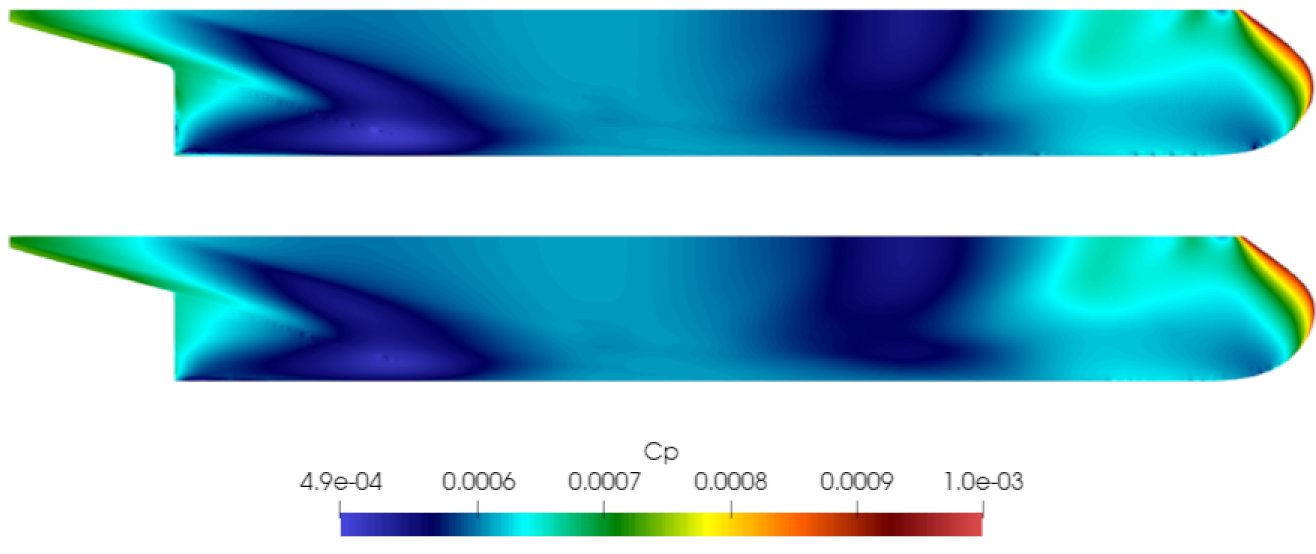
\includegraphics[width=.6\columnwidth]{./images/cp_lateral2.png}
\caption{$C_P$ para $Fr=0.2$, vista lateral. Arriba: escala 1:20. Abajo: 
escala 1:1.}
\label{cp_side}
\end{figure}

Los resultados indican que la recuperación de presión en la zona de popa es 
considerablemente menor que en cascos más hidrodinámicos, como el KCS 
\citep{cp_recovery_kcs}, lo cual explica los altos valores de $(1+k)$ 
observados en este tipo de buques. En cuanto al efecto del número de 
Reynolds sobre $C_P$, se observa una diferencia muy leve en la distribución 
de presiones en la zona de popa entre escalas: la presión en escala 1:1 
recupera ligeramente más que en escala 1:20, lo cual es consistente con la 
disminución muy leve de $C_{PV}$ con $Re$ observada para este buque.

Las Figuras~\ref{fig:cp_z0}, \ref{fig:cp_z5} y \ref{fig:cp_z75} presentan la 
distribución longitudinal del coeficiente de presión $C_{P}(x/L)$ para 
distintos números de Reynolds, sobre tres planos horizontales a profundidad 
constante $z/T = 0$, $0.5$ y $0.75$ respectivamente, es decir, en la línea de 
flotación, a media manga sumergida y cerca del fondo. La coordenada 
longitudinal se expresa como $x/L$, donde $x/L = 0$ corresponde a la 
perpendicular de proa. Se observa un déficit persistente de presión en la 
región de popa para todos los $Re$, en las tres líneas de agua analizadas, 
con variaciones mínimas entre escalas. La diferencia entre el caso a escala 
modelo ($Re=1.3\times10^6$) y el de escala buque ($Re=1.1\times10^8$) es del 
orden de $\Delta C_P = 0.01$--$0.02$, lo que indica que la recuperación de 
presión en popa es extremadamente débil y poco sensible a los efectos 
inerciales del flujo. Estos resultados cuantitativos son plenamente 
consistentes con la lenta disminución de $C_{PV}$ con el número de Reynolds, 
respaldando la conclusión de que las pérdidas por presión viscosa en la 
región de popa dominan el comportamiento del factor de forma $(1+k)$ para 
este casco.

\begin{figure}[htpb]
    \centering
    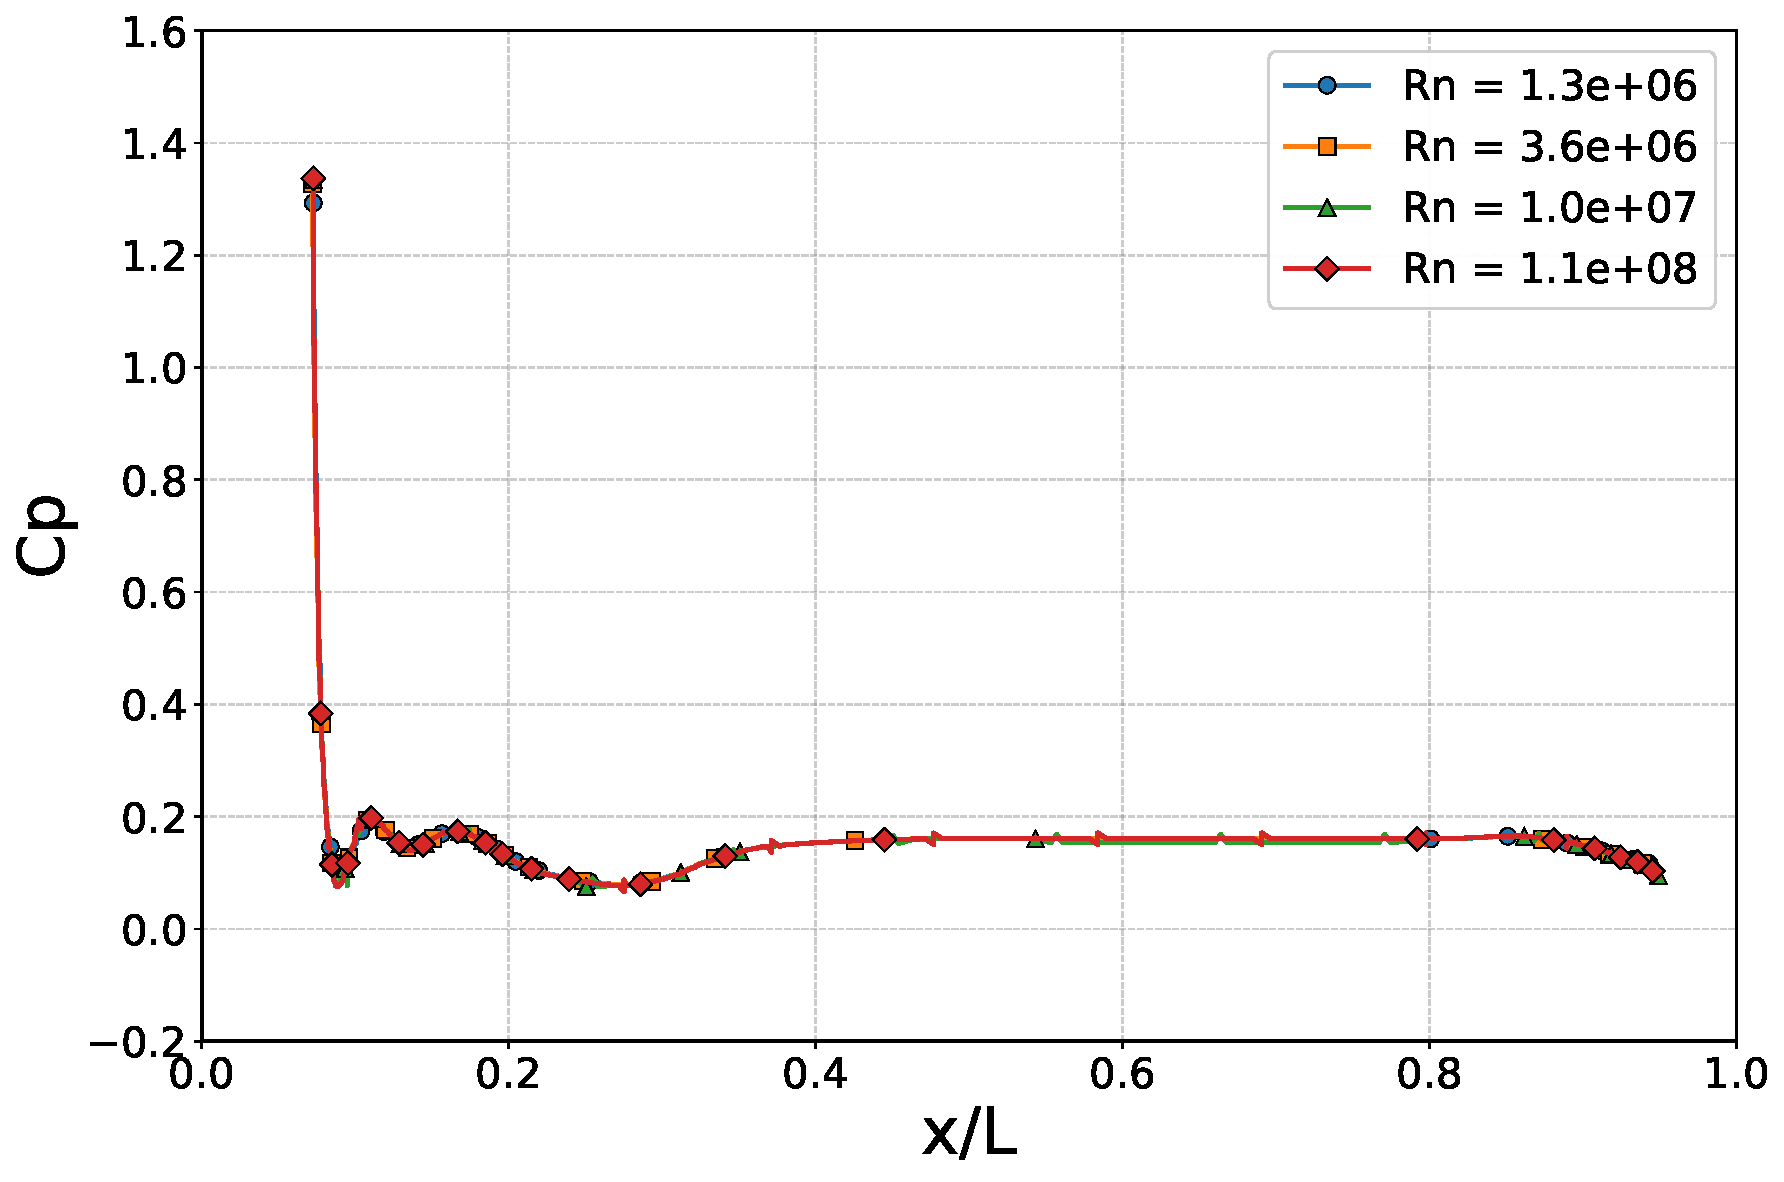
\includegraphics[width=.6\columnwidth]{./images/z0.pdf}
    \caption{Distribución de $C_{P}(x/L)$ sobre el plano $z/T = 0$ 
    (línea de flotación). Se observa un déficit persistente de presión 
    en popa y variaciones mínimas entre escalas.}
    \label{fig:cp_z0}
\end{figure}

\begin{figure}[htpb]
    \centering
    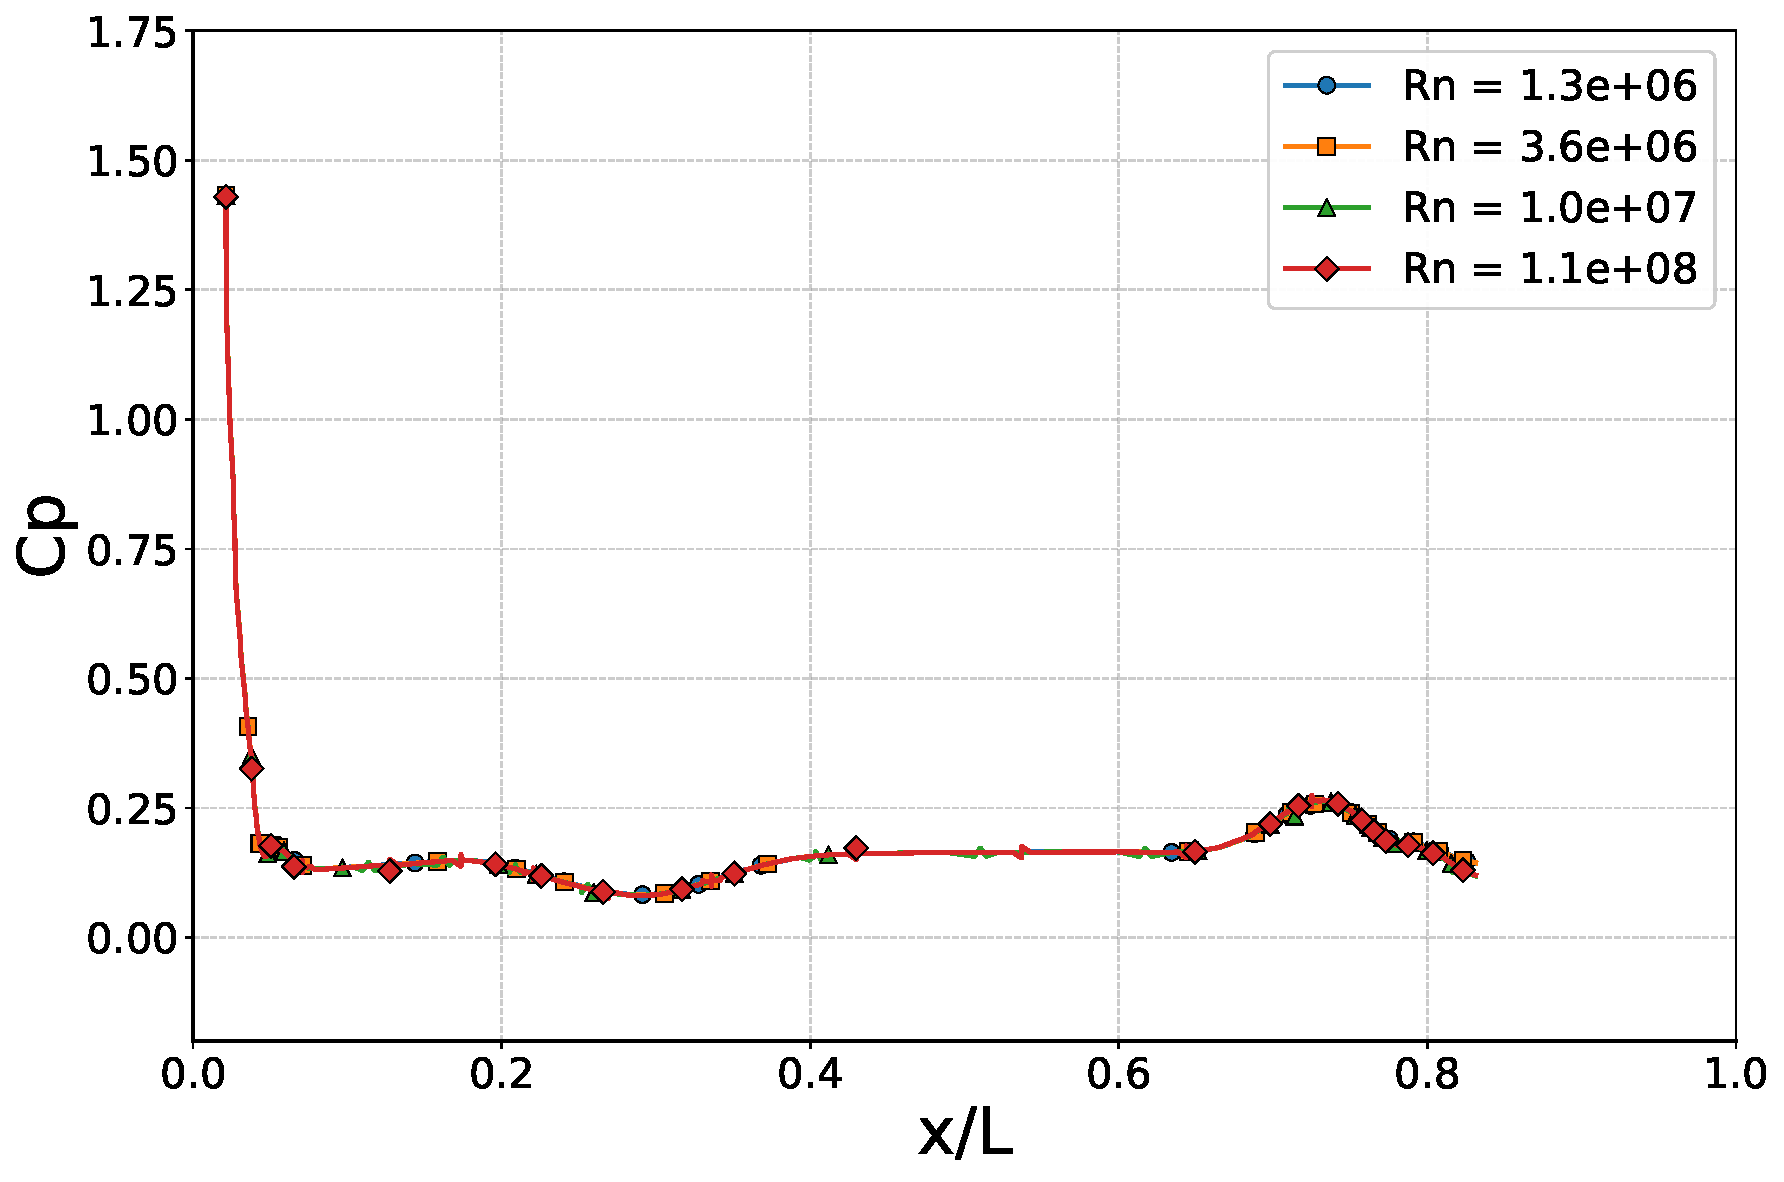
\includegraphics[width=.6\columnwidth]{./images/z5.pdf}
    \caption{Distribución de $C_{P}(x/L)$ sobre el plano $z/T = 0.5$.}
    \label{fig:cp_z5}
\end{figure}

\begin{figure}[htpb]
    \centering
    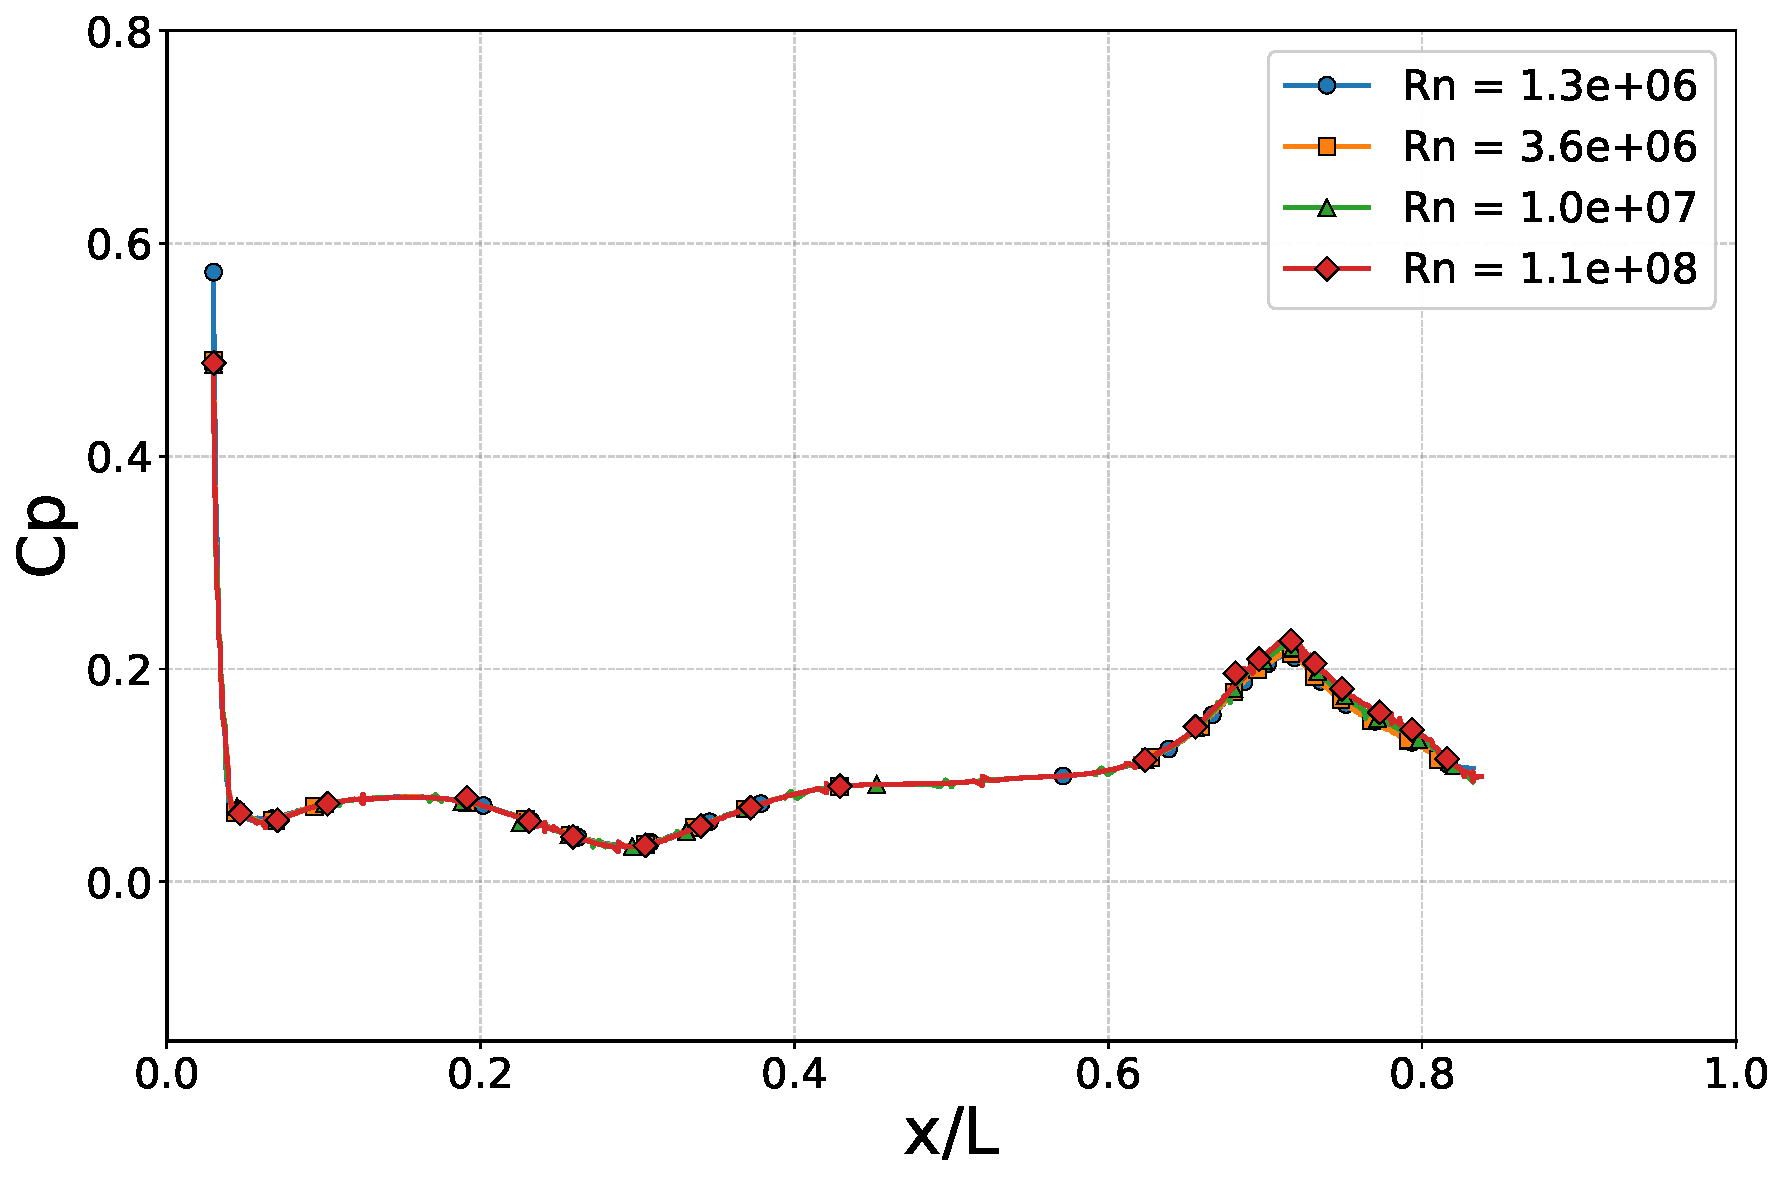
\includegraphics[width=.6\columnwidth]{./images/z75.pdf}
    \caption{Distribución de $C_{P}(x/L)$ sobre el plano $z/T = 0.75$.}
    \label{fig:cp_z75}
\end{figure}


\subsection{Conclusiones parciales}

El análisis de la distribución del coeficiente de presión $C_P$ confirma que 
el comportamiento del término de presión viscosa $C_{PV}$ está dominado por 
la región de popa del \textit{P1}. En todas las escalas analizadas se 
observa una recuperación de presión muy limitada en el cuerpo de salida, lo 
que conduce a pérdidas viscosas significativas asociadas a gradientes de 
presión adversos y a la persistencia de estructuras vorticosas de gran 
escala.

La comparación entre escala modelo y escala buque muestra que el efecto del 
número de Reynolds sobre la distribución de presiones es reducido. Si bien a 
escala buque se aprecia una recuperación de presión levemente mayor, las 
diferencias cuantitativas son pequeñas y se traducen únicamente en una 
disminución muy moderada de $C_{PV}$. Como se discutió en la 
Sección~\ref{sec:descomposicion_de_la_res_viscosa}, esta leve disminución 
puede atribuirse al efecto del adelgazamiento de la capa límite tridimensional con $Re$, mientras que la persistencia de las estructuras vorticosas de popa, prácticamente estables con la escala, explica que dicha disminución sea tan moderada. Este resultado explica la débil dependencia de la presión viscosa con $Re$ observada previamente y, en consecuencia, el crecimiento sostenido del factor de forma $(1+k)$ con la escala.

El déficit persistente de presión en popa, prácticamente invariante con el 
número de Reynolds, constituye así el mecanismo físico principal que 
distingue a los cascos de baja esbeltez de los cascos esbeltos convencionales. 
En este tipo de geometrías, las pérdidas por presión viscosa dominan la 
resistencia viscosa total y limitan la validez de los supuestos clásicos de 
extrapolación, reforzando la necesidad de considerar explícitamente los 
efectos geométricos en la estimación del factor de forma.

\section{Influencia de la proa bulbo en el factor de forma}\label{sec:proa_bulbo}

\subsection{Motivación y antecedentes sobre proa bulbo en pesqueros}

La incorporación de una proa bulbo en cascos pesqueros suele tener dos 
objetivos. Por un lado, aumentar el desplazamiento del casco, siendo esta 
una de las únicas variables disponibles dadas las limitaciones de eslora 
establecidas por las reglamentaciones nacionales. Por otro lado, busca 
reducir la resistencia por formación de olas en el rango de velocidades de 
servicio, mediante la generación de un sistema de ondas que interfiera 
destructivamente con el tren de olas producido por el resto del casco.

Como se discutió en la Sección~\ref{sec:prohaska_antec}, 
\citet{korkmaz_cfd_2021} reportaron que la geometría de la proa bulbo puede 
tener un impacto significativo en la aplicabilidad del método de Prohaska, 
llegando a introducir curvaturas marcadas en el diagrama que obligan a 
restringir severamente el rango de $Fr$ analizado, o incluso a descartar el 
método. El efecto se atribuye a la proximidad del bulbo a la superficie 
libre, que genera un sistema de ondas propio cuya interacción con el tren de 
proa no responde a la ley $Fr^4$ supuesta por el método.

El \textit{P1} presenta ambas anomalías: la curvatura cóncava a bajos 
números de Froude en su diagrama de Prohaska 
(Sección~\ref{sec:det_num_fac_form}) y la ausencia de un valor asintótico de 
$(1+k)$ con la velocidad y con la escala 
(Sección~\ref{sec:analisis_efectos_escala}), en contraste con el 
comportamiento del KCS. Ambas observaciones motivan la pregunta de 
investigación que organiza esta sección: \textit{¿es la proa bulbo 
responsable, total o parcialmente, de dichas anomalías?} Para responderla se 
repite el procedimiento completo de determinación del factor de forma sobre 
una variante del casco sin bulbo, de modo que cualquier comportamiento que 
persista en esa configuración no pueda atribuirse a su presencia.

\subsection{Modelos numéricos}

Para aislar el efecto del bulbo se generó un modelo modificado del 
\textit{P1} a escala 1:20, denominado ``Ctrl+Z'' en alusión al comando de 
deshacer, en referencia a que revierte la tendencia actual de incorporar 
proas bulbo en el diseño de pesqueros. El criterio de modificación consistió 
en eliminar el bulbo del modelo original manteniendo sin cambios el resto de 
la geometría del casco, de modo que ambos modelos resulten comparables y la 
única diferencia entre ellos sea la presencia o ausencia del bulbo. Este 
análisis se realizó exclusivamente a escala modelo, en una etapa temprana de 
la investigación, previa a la extensión del estudio a escalas mayores 
presentada en la Sección~\ref{sec:analisis_efectos_escala}.

Dado que el bulbo se encuentra completamente sumergido, su eliminación no 
modifica la eslora de flotación, que permanece idéntica en ambas 
configuraciones y define por lo tanto un mismo número de Froude para una 
misma velocidad. Sí se modifica, en cambio, la eslora mojada, que se reduce 
de $1{.}634$ a $1{.}515$~m para $T = 0{.}165$~m y de $1{.}641$ a $1{.}575$~m 
para $T = 0{.}195$~m. Esta distinción es relevante porque es la eslora 
mojada la que interviene en el número de Reynolds y, en consecuencia, en el 
coeficiente de fricción de referencia $C_{F0}$ empleado para la 
descomposición: a igual velocidad, la configuración con bulbo opera a un 
$Re$ mayor y por lo tanto a un $C_{F0}$ menor. Todas las comparaciones 
presentadas a continuación se realizan a igual número de Froude, es decir, a 
igual velocidad, empleando para cada configuración su propia eslora mojada 
en el cálculo de $Re$.

La Figura~\ref{fig:tpa_y_ctrlZ} presenta, para ambos modelos, la vista de 
perfil con la curva de áreas superpuesta (en rojo) y la vista en perspectiva 
del casco. La curva de áreas representa el área de la sección transversal 
sumergida en función de la posición longitudinal, y permite visualizar de 
manera directa cómo se modifica la distribución de volumen del casco al 
eliminar el bulbo: en el modelo original (Figura~\ref{fig:tpa_y_ctrlZ}a) se 
observa el incremento de área característico en la zona de proa asociado al 
bulbo, mientras que en el modelo Ctrl+Z (Figura~\ref{fig:tpa_y_ctrlZ}b) dicha 
protuberancia desaparece, conservándose el resto de la distribución de 
volumen prácticamente sin cambios.

\begin{figure}
    \centering
    \begin{subfigure}{\linewidth}
        \centering
        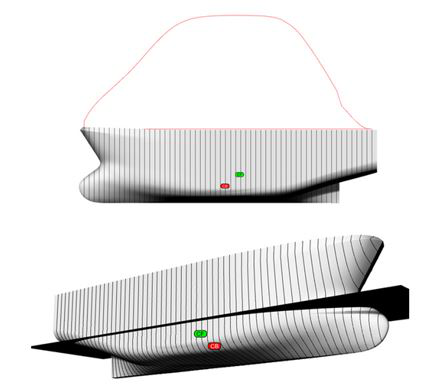
\includegraphics[width=.6\columnwidth]{./images/A1.png}
        \caption{Modelo original.}
    \end{subfigure}

    \vspace{1em}

    \begin{subfigure}{\linewidth}
        \centering
        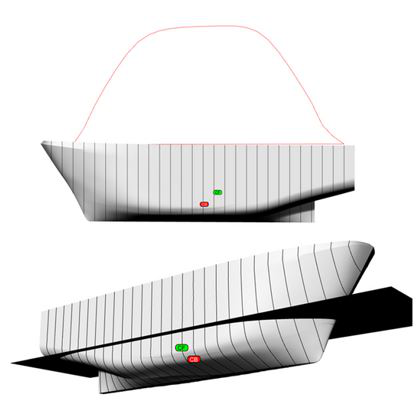
\includegraphics[width=.6\columnwidth]{./images/A2.png}
        \caption{Modelo Ctrl+Z.}
    \end{subfigure}

    \caption{Comparación entre el modelo original del \textit{P1} y el 
    modelo Ctrl+Z, sin proa bulbo, junto con sus curvas de áreas 
    correspondientes (en rojo).}
    \label{fig:tpa_y_ctrlZ}
\end{figure}


\subsection{Resultados de resistencia para diferentes configuraciones de proa 
en todo el rango de operación}

Para evaluar el impacto de la proa bulbo sobre la resistencia del 
\textit{P1}, se compararon las curvas de resistencia total ($C_T$), viscosa 
($C_V$) y por olas ($C_W$) en función del número de Froude, para los dos 
modelos (con y sin bulbo) y los dos calados disponibles ($T = 0{.}165$~m y 
$T = 0{.}195$~m). El coeficiente $C_T$ se obtuvo directamente de las 
simulaciones bifásicas con superficie libre para cada configuración. El 
coeficiente $C_V$ se calculó como:
%
\begin{equation}
    C_V = (1+k)\, C_{F0}
\end{equation}
%
empleando, para cada configuración, el factor de forma $k$ determinado 
mediante el método de Prohaska a partir de sus propias simulaciones CFD 
bifásicas: para el modelo original con bulbo, el valor validado contra el 
ensayo experimental (Sección~\ref{sec:det_exp_fac_form}); para el modelo 
Ctrl+Z, el valor obtenido aplicando el mismo procedimiento a sus 
simulaciones, sin contar con un ensayo experimental propio de validación. 
Finalmente, el coeficiente de resistencia por olas se obtuvo como residuo:
%
\begin{equation}
    C_W = C_T - C_V
\end{equation}

Los diagramas de Prohaska correspondientes a ambas configuraciones se 
presentan en las Figuras~\ref{fig:prohaska_bulbo_165} y 
\ref{fig:prohaska_bulbo_195}. En ambos calados se observa que la curvatura 
cóncava a bajos números de Froude, ya identificada para el modelo original 
en la Sección~\ref{sec:det_num_fac_form}, se reproduce con igual intensidad 
en la configuración Ctrl+Z. Este resultado permite descartar la primera de 
las hipótesis planteadas: la deformación del diagrama de Prohaska no 
responde a la presencia del bulbo, sino que constituye una característica 
propia del resto del casco. La anomalía reportada por 
\citet{korkmaz_cfd_2021} para cascos con bulbo próximo a la superficie libre 
no explica, por lo tanto, el comportamiento observado en el \textit{P1}.

Descartada la proa bulbo, subsisten dos de las causas enumeradas en la 
Sección~\ref{sec:prohaska_antec}: la geometría del resto del casco y el 
modelado numérico de la zona de transición. Ambas configuraciones fueron 
simuladas con el mismo cierre turbulento ($k$--$\omega$ SST) y operan en el 
mismo rango de números de Reynolds, de modo que la comparación entre ellas 
no permite discriminar entre ambos orígenes: el adelantamiento del punto de 
transición que introduce un modelo formulado para régimen enteramente 
turbulento, discutido en la Sección~\ref{sec:det_num_fac_form}, afecta por 
igual a los dos casos y no puede aislarse eliminando el bulbo.

Existe, no obstante, un indicio a favor del origen numérico. Como se señaló 
en la Sección~\ref{sec:det_num_fac_form}, la desviación observada en los 
ensayos experimentales es convexa, mientras que la de las simulaciones es 
cóncava. Este cambio de signo sugiere que la concavidad no reproduce un 
fenómeno físico del casco sino que constituye un artefacto de la 
simulación, asociado a la incapacidad del modelo de turbulencia empleado 
para representar la fracción de capa límite que permanece laminar a los 
$Re$ de escala modelo. Dirimir definitivamente esta cuestión requeriría 
repetir las simulaciones con un modelo de transición del tipo 
$\gamma$--$\widetilde{Re}_{\theta t}$ (Sección~\ref{sec:modelos_transicion}), 
lo que excede el alcance de esta sección y queda planteado como línea de 
trabajo futuro.

\begin{figure}[htpb]
	\centering
	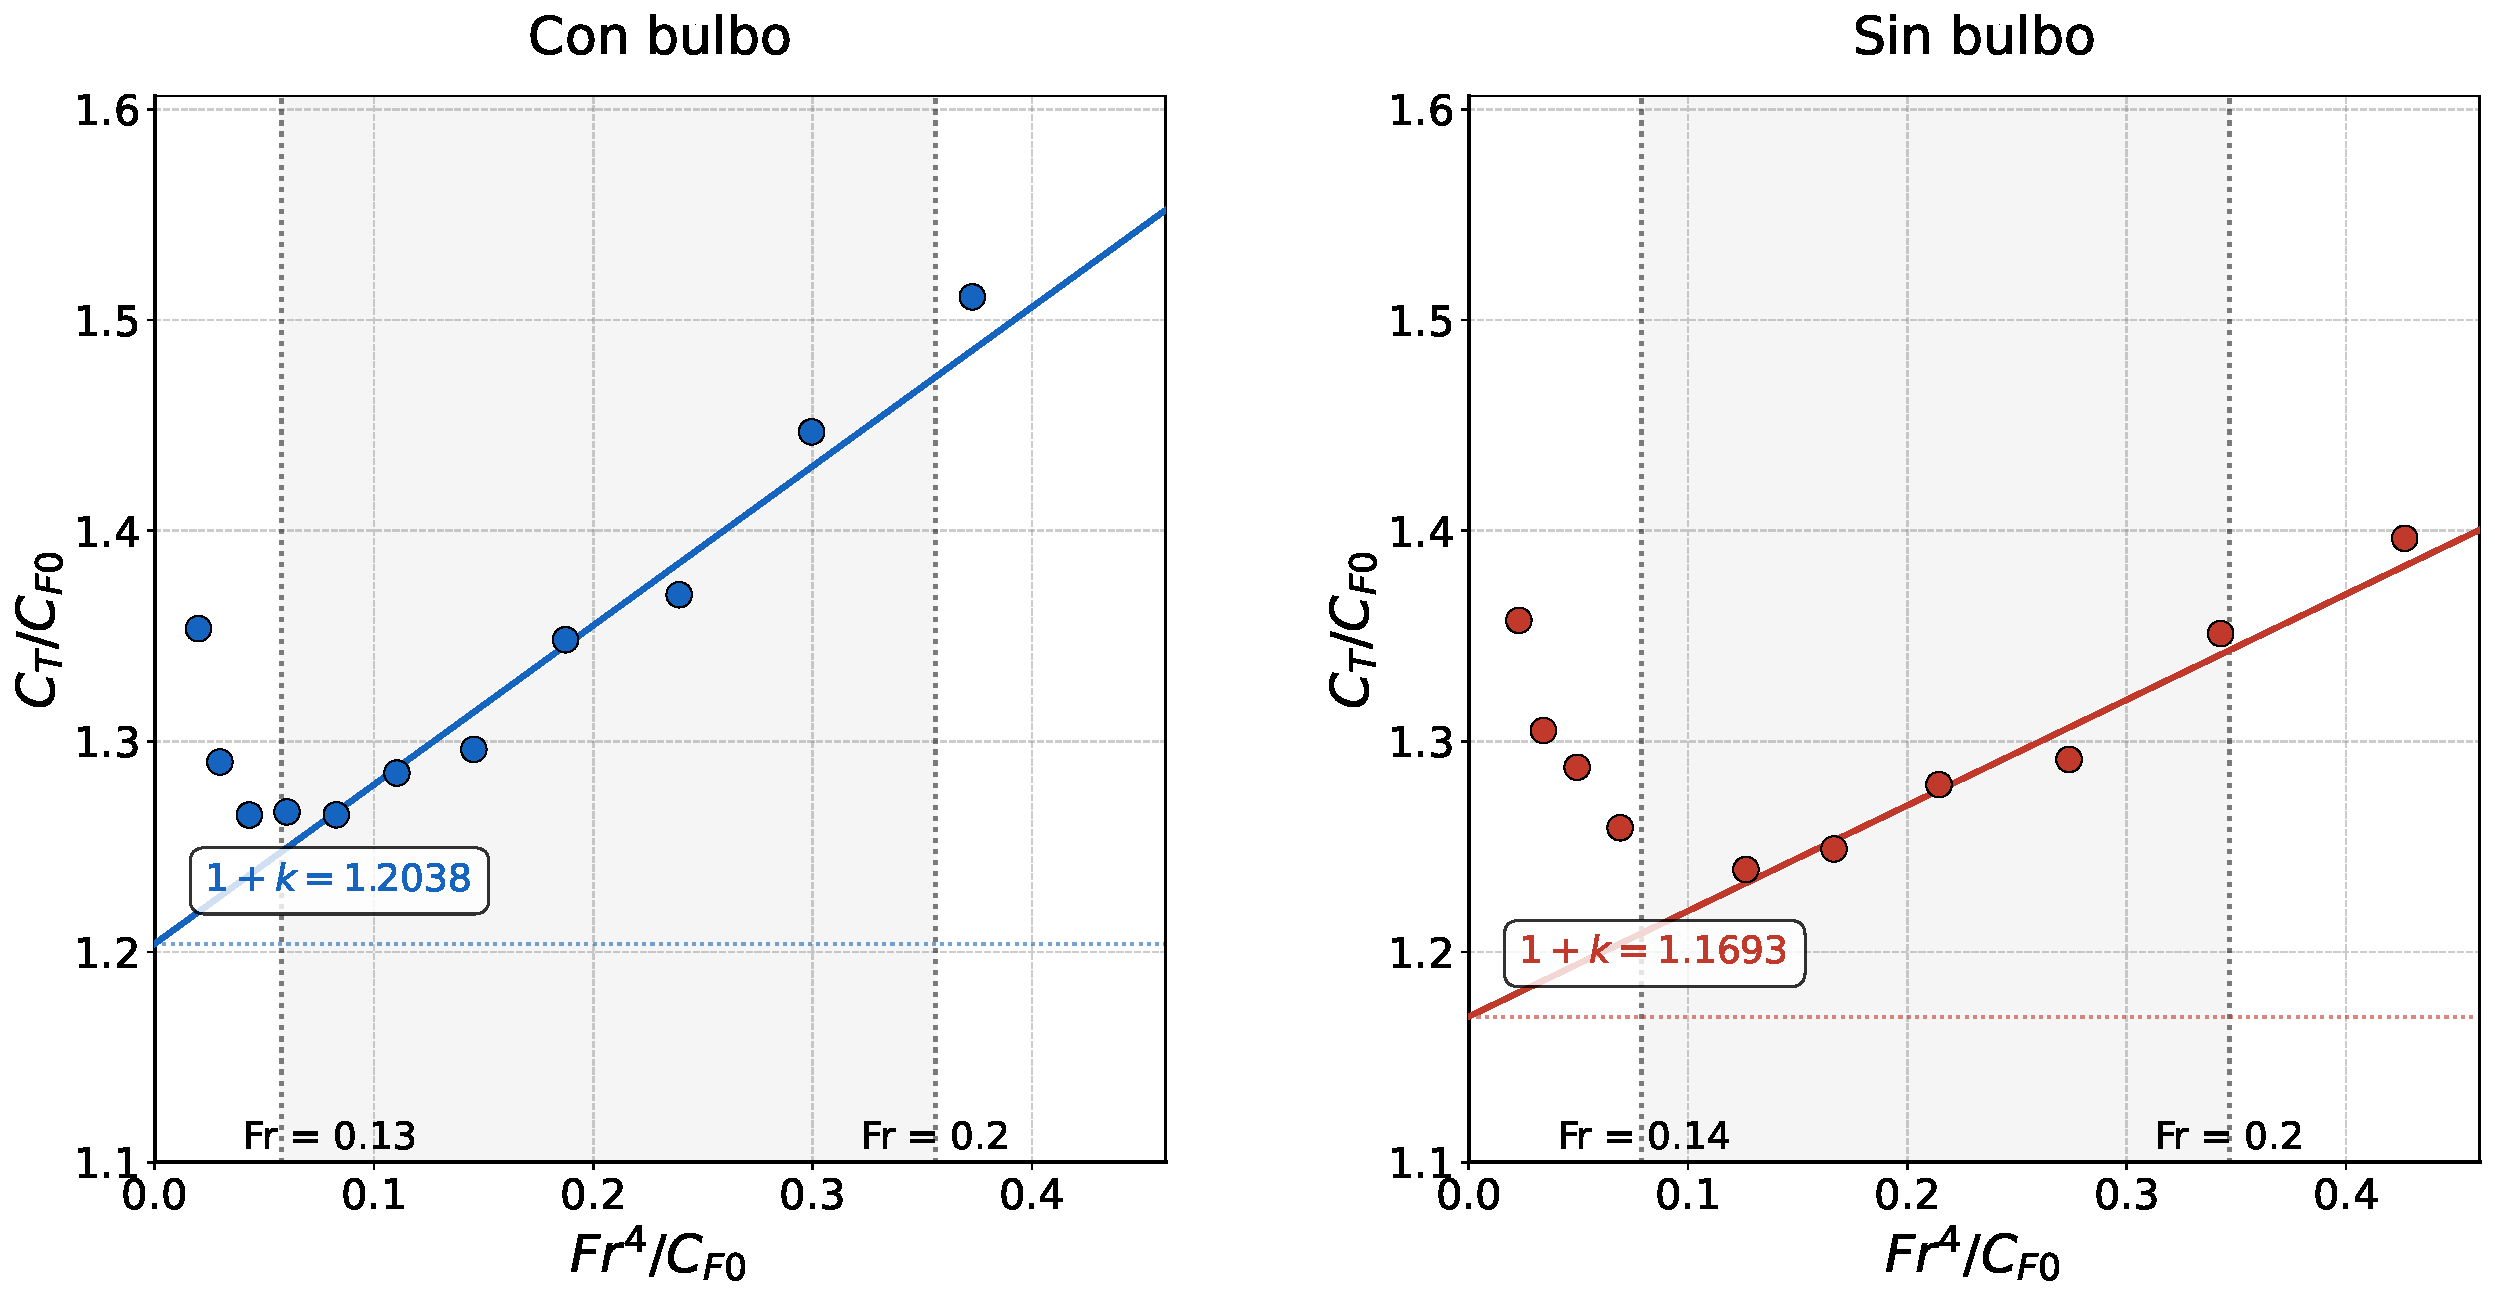
\includegraphics[width=.9\textwidth]{images/prohaska-bulbo-ctrlz-165.pdf}
	\caption{Diagrama de Prohaska comparando modelos con y sin bulbo 
	($T = 0{.}165$~m).}
	\label{fig:prohaska_bulbo_165}
\end{figure}

\begin{figure}[htpb]
	\centering
	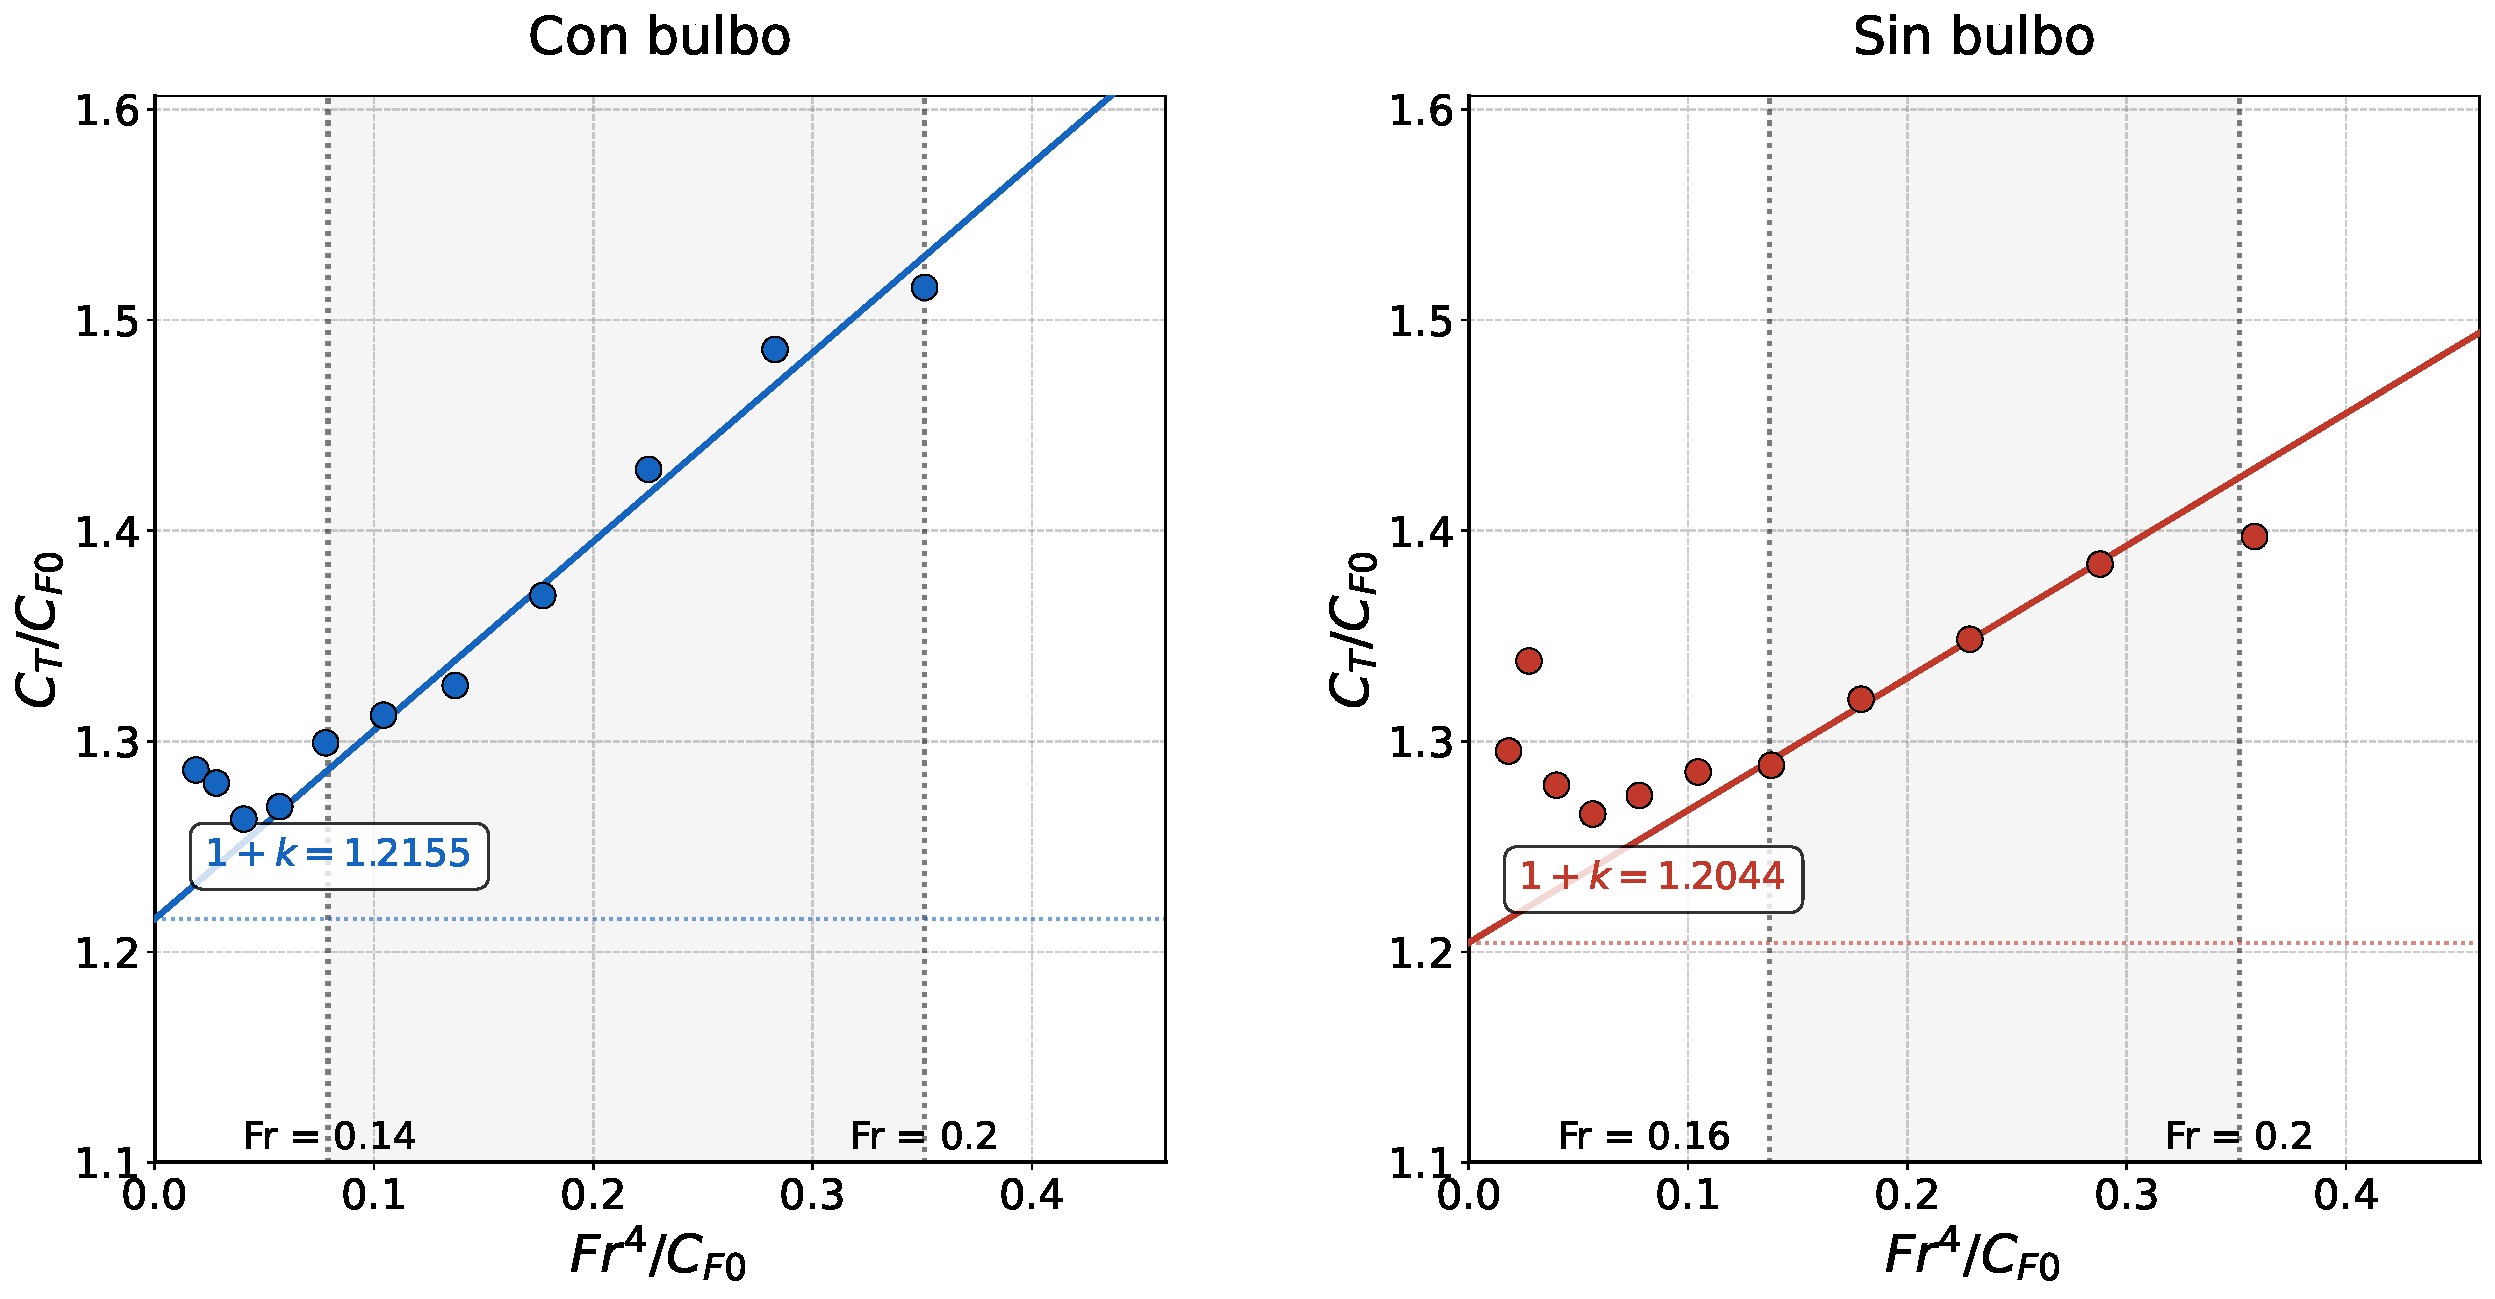
\includegraphics[width=.9\textwidth]{images/prohaska-bulbo-ctrlz-195.pdf}
	\caption{Diagrama de Prohaska comparando modelos con y sin bulbo 
	($T = 0{.}195$~m).}
	\label{fig:prohaska_bulbo_195}
\end{figure}

\paragraph{Calado $T = 0{.}165$~m} La Figura~\ref{fig:Ct_bulbo_165} muestra 
que la configuración con bulbo reduce la resistencia total a partir de 
$Fr \approx 0{.}25$, coincidiendo con la velocidad de diseño del bulbo. Por 
debajo de dicho valor ambas curvas se mantienen dentro de $5\times10^{-4}$ 
en $C_T$, sin diferencias apreciables entre configuraciones, con la 
excepción del punto $Fr \approx 0{.}24$, inmediatamente anterior al cruce, 
donde la configuración con bulbo presenta un incremento localizado de la 
resistencia total. La Figura~\ref{fig:Cw_bulbo_165} muestra que la mejora 
observada a velocidades altas se explica por una reducción de la resistencia 
por olas en ese mismo rango, consistente con la función destructiva esperada 
del bulbo. La Figura~\ref{fig:Cv_bulbo_165} muestra que la resistencia 
viscosa de la configuración con bulbo resulta levemente superior en todo el 
rango, entre un $1$ y un $1{.}5$\,\%, diferencia reducida pero de signo 
constante y consistente con el mayor factor de forma determinado para esta 
configuración.

\begin{figure}[htpb]
    \centering
    \begin{subfigure}[b]{0.48\textwidth}
        \centering
        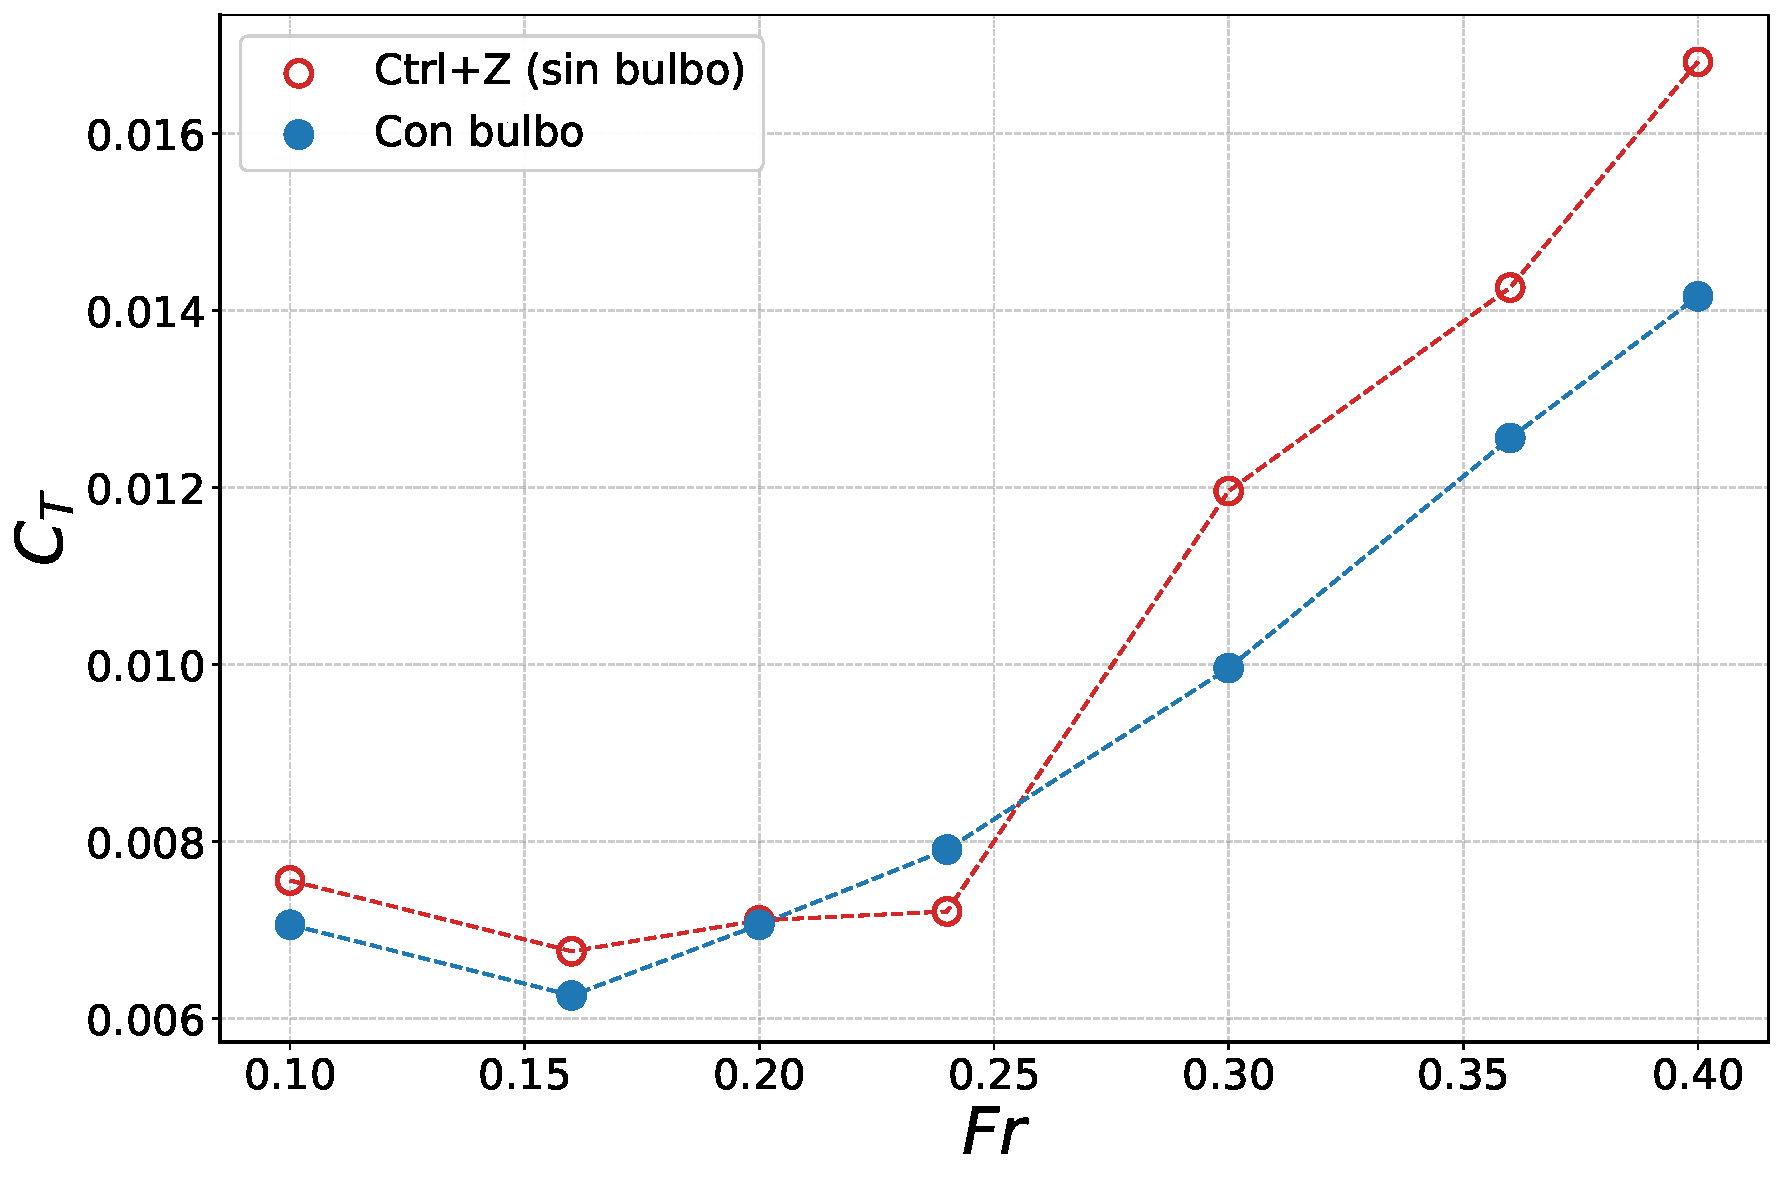
\includegraphics[width=\textwidth]{images/Ct-consinbulbo-165.pdf}
        \caption{Resistencia total.}
        \label{fig:Ct_bulbo_165}
    \end{subfigure}
    \hfill
    \begin{subfigure}[b]{0.48\textwidth}
        \centering
        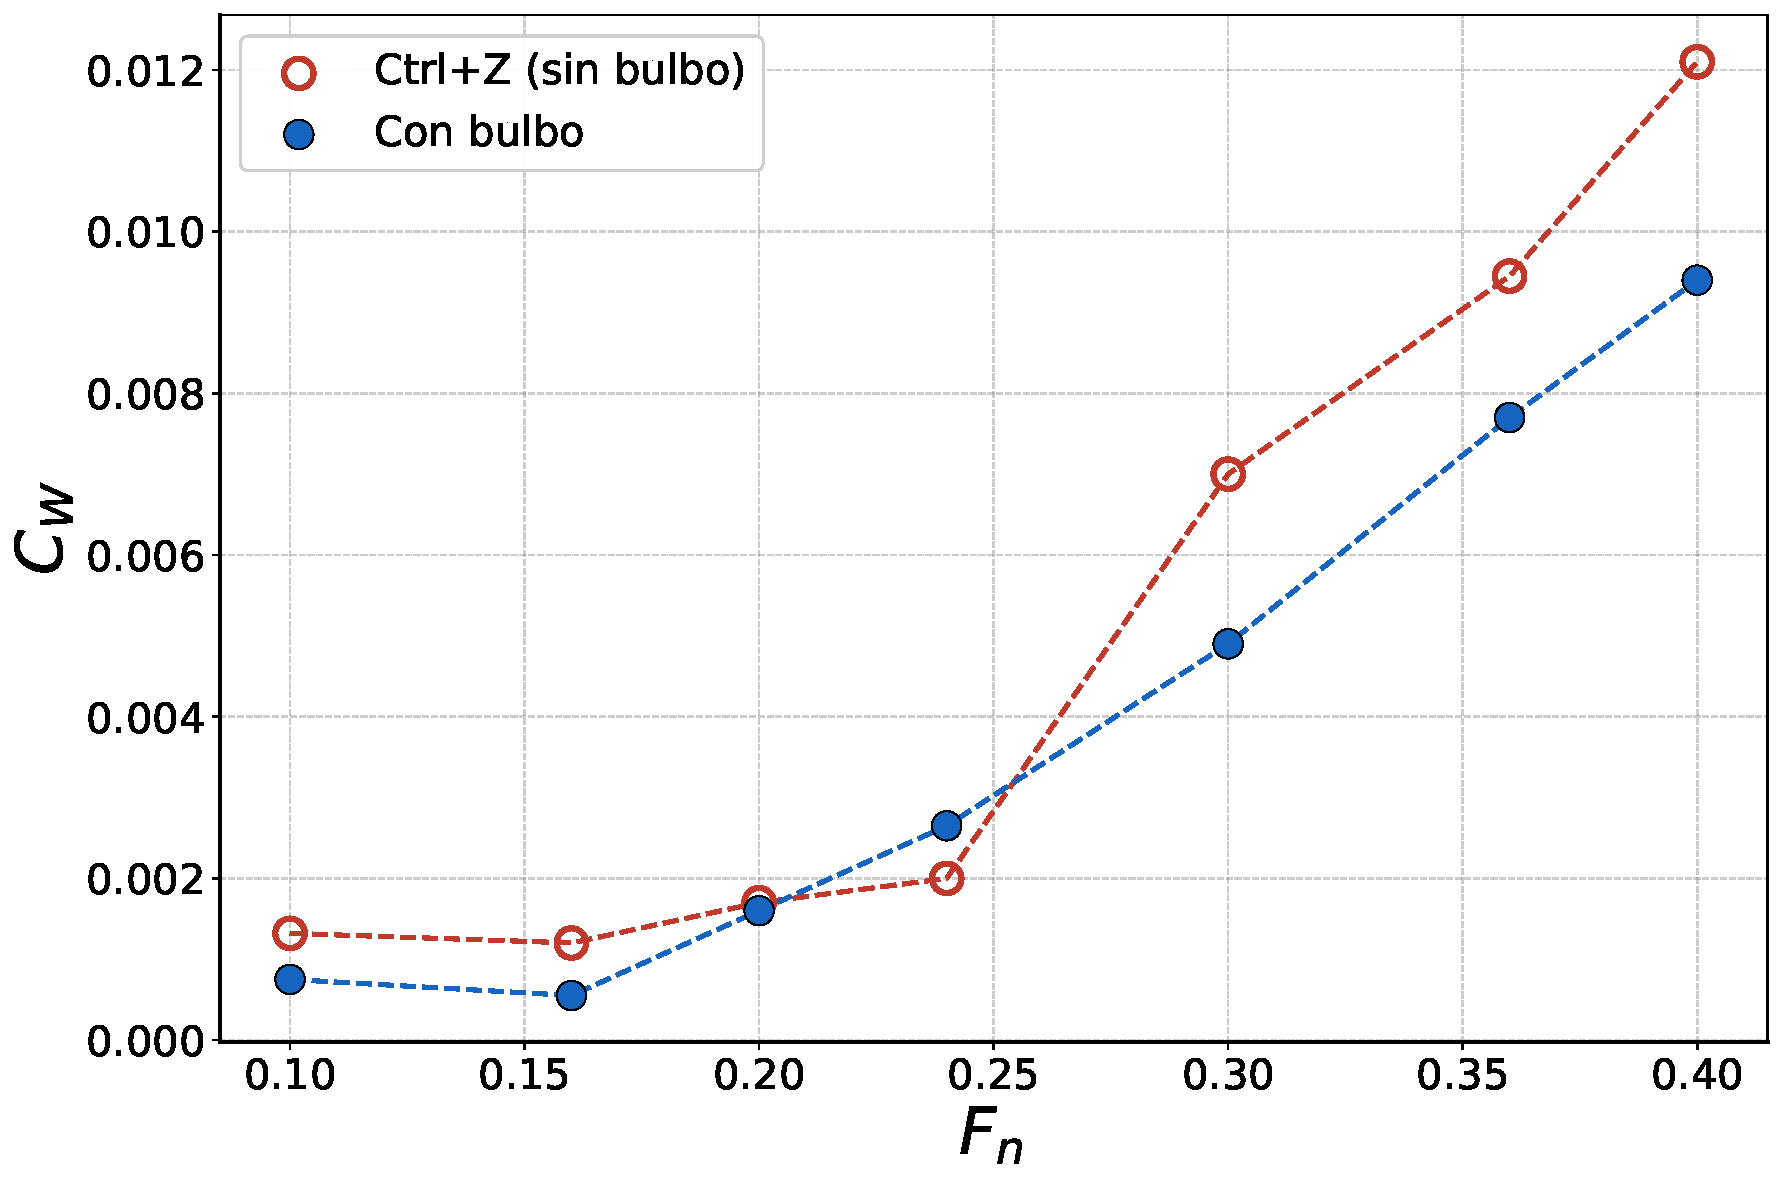
\includegraphics[width=\textwidth]{images/Cw-consinbulbo-165.pdf}
        \caption{Resistencia por olas.}
        \label{fig:Cw_bulbo_165}
    \end{subfigure}

    \vspace{0.6cm}

    \begin{subfigure}[b]{0.48\textwidth}
        \centering
        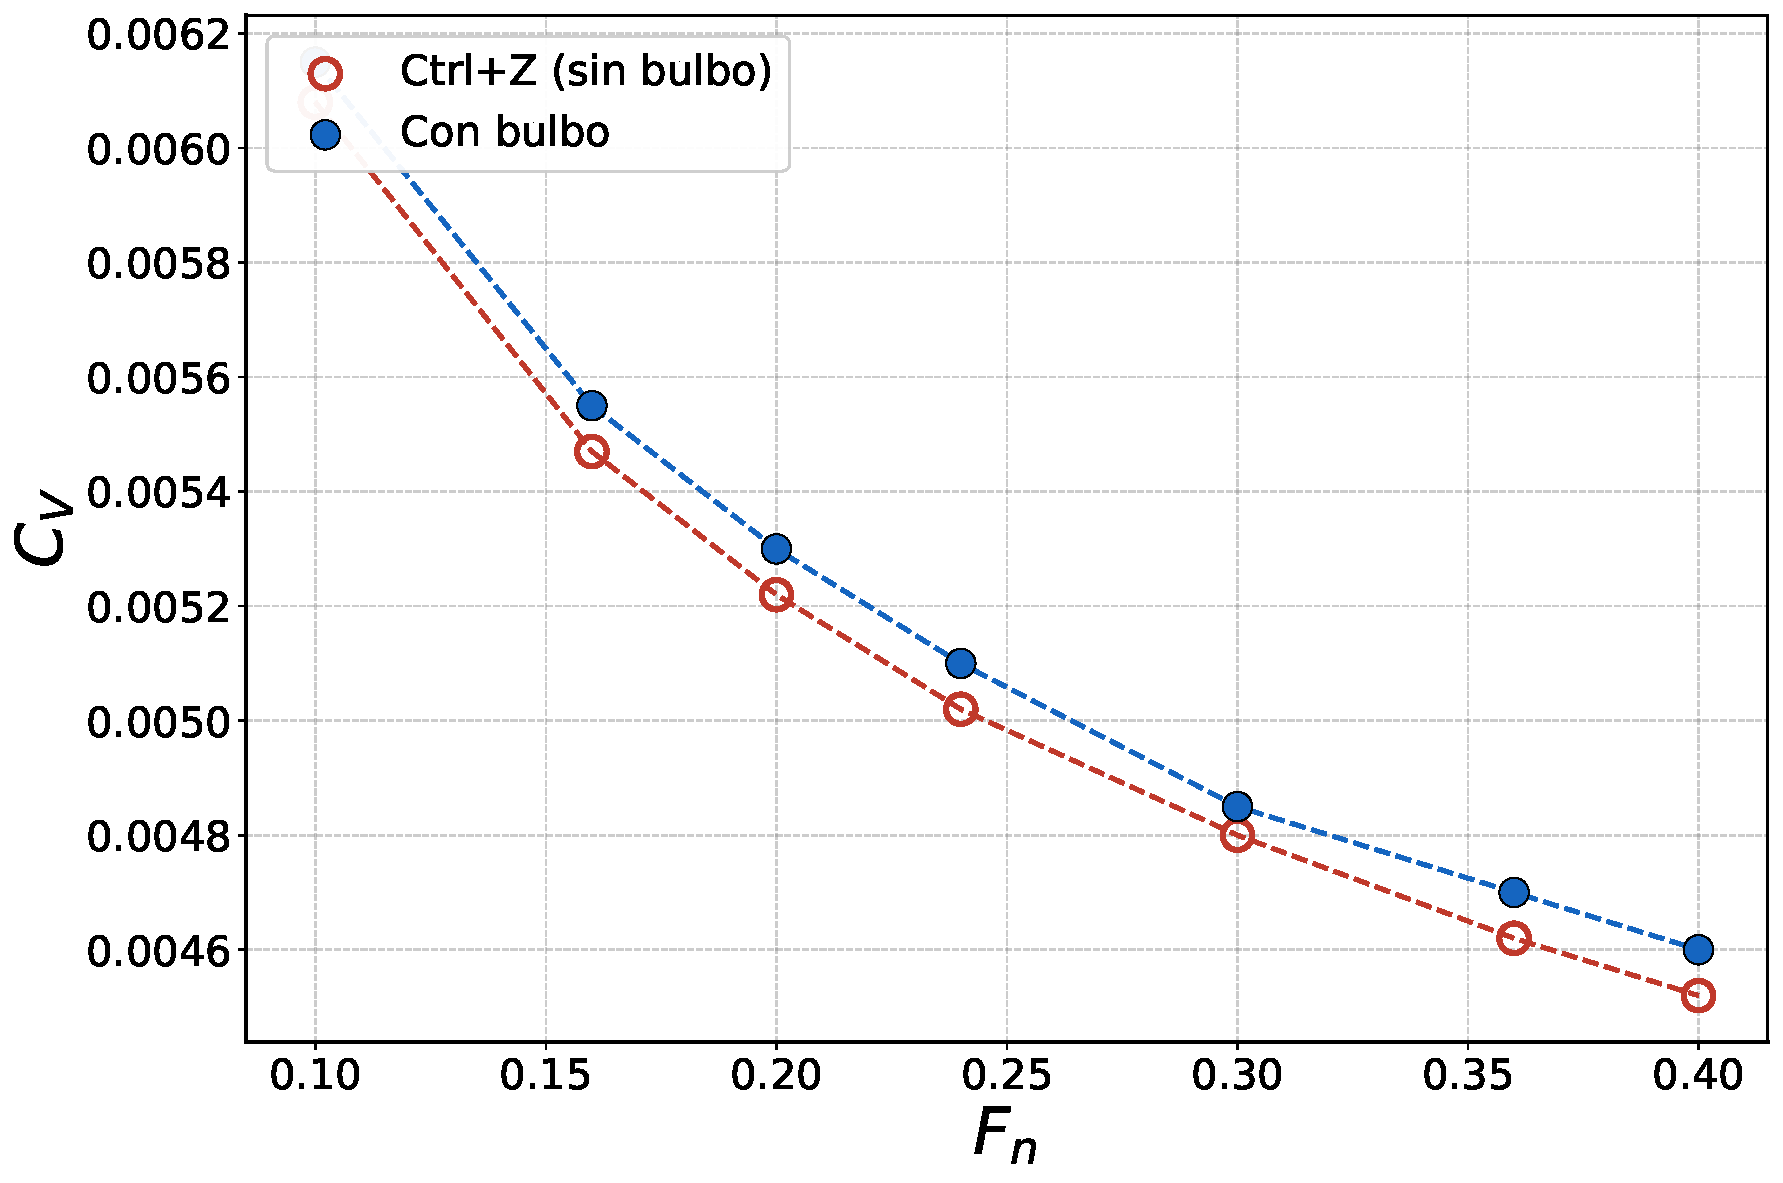
\includegraphics[width=\textwidth]{images/Cv-consinbulbo-165.pdf}
        \caption{Resistencia viscosa.}
        \label{fig:Cv_bulbo_165}
    \end{subfigure}

    \caption{Descomposición de la resistencia del \textit{P1} con y sin proa 
    bulbo para el calado $T = 0{.}165$~m.}
    \label{fig:coef_bulbo_165}
\end{figure}

\paragraph{Calado $T = 0{.}195$~m} Para este calado, la 
Figura~\ref{fig:Ct_bulbo_195} muestra que la configuración con bulbo no 
presenta una mejora neta en resistencia total: la diferencia entre ambas 
curvas oscila a lo largo del rango sin definir una tendencia, alternando 
tramos favorables y desfavorables al bulbo. La 
Figura~\ref{fig:Cv_bulbo_195} muestra que las resistencias viscosas de ambas 
configuraciones resultan prácticamente indistinguibles, de modo que la 
diferencia observada en $C_T$ se explica enteramente por la componente de 
olas. En efecto, la Figura~\ref{fig:Cw_bulbo_195} muestra que el bulbo 
reduce $C_W$ en el entorno de $Fr \approx 0{.}20$--$0{.}30$, pero pierde 
ese beneficio por encima de $Fr \approx 0{.}35$, donde la tendencia se 
invierte y la configuración con bulbo pasa a presentar una resistencia por 
olas superior a la del casco desnudo.

Este comportamiento resulta consistente con la mayor sumergencia del bulbo a 
este calado. Al aumentar su distancia a la superficie libre se modifica el 
sistema de ondas que genera, tanto en amplitud como en fase, de manera que 
la interferencia destructiva con el tren de olas del casco deja de resultar 
favorable en el extremo alto del rango de operación. El beneficio 
hidrodinámico del bulbo aparece así como fuertemente dependiente de la 
condición de carga.

\begin{figure}[htpb]
    \centering
    \begin{subfigure}[b]{0.48\textwidth}
        \centering
        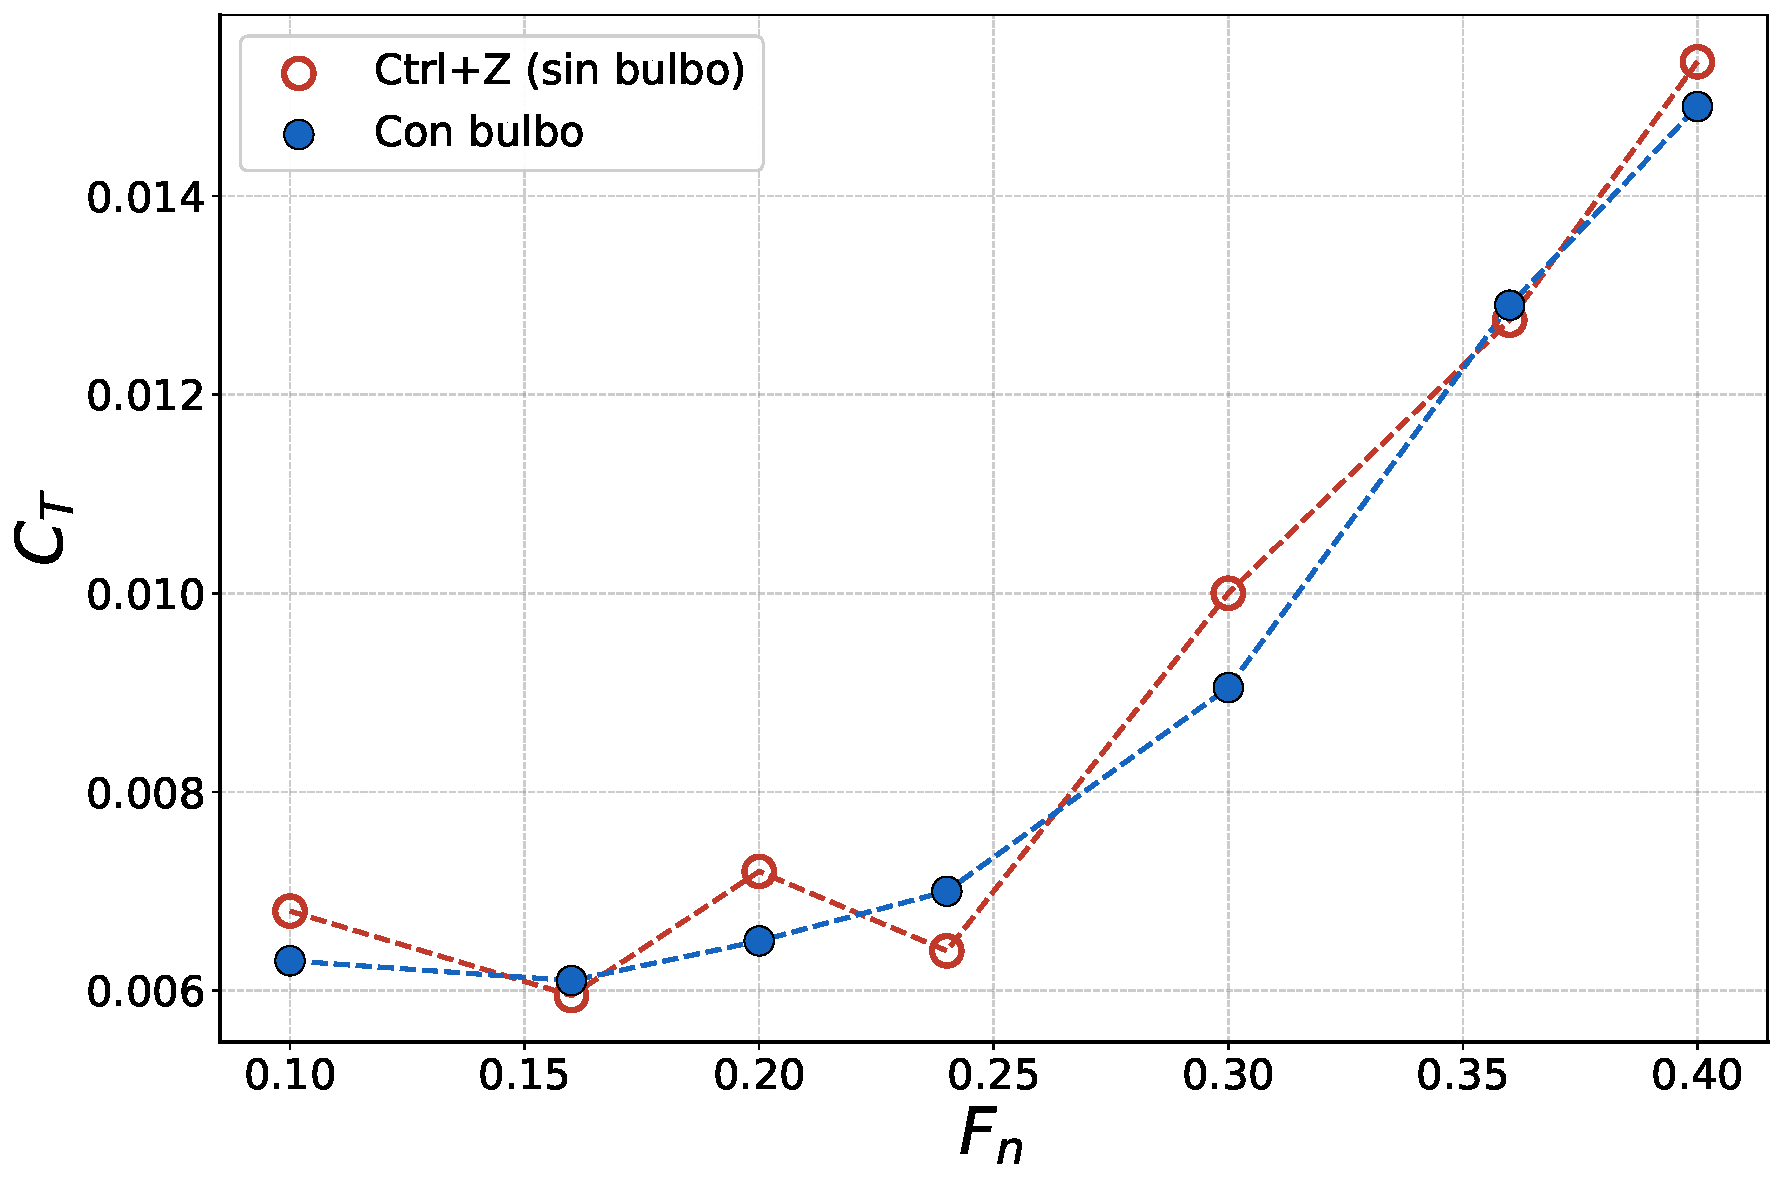
\includegraphics[width=\textwidth]{images/Ct-consinbulbo-195.pdf}
        \caption{Resistencia total.}
        \label{fig:Ct_bulbo_195}
    \end{subfigure}
    \hfill
    \begin{subfigure}[b]{0.48\textwidth}
        \centering
        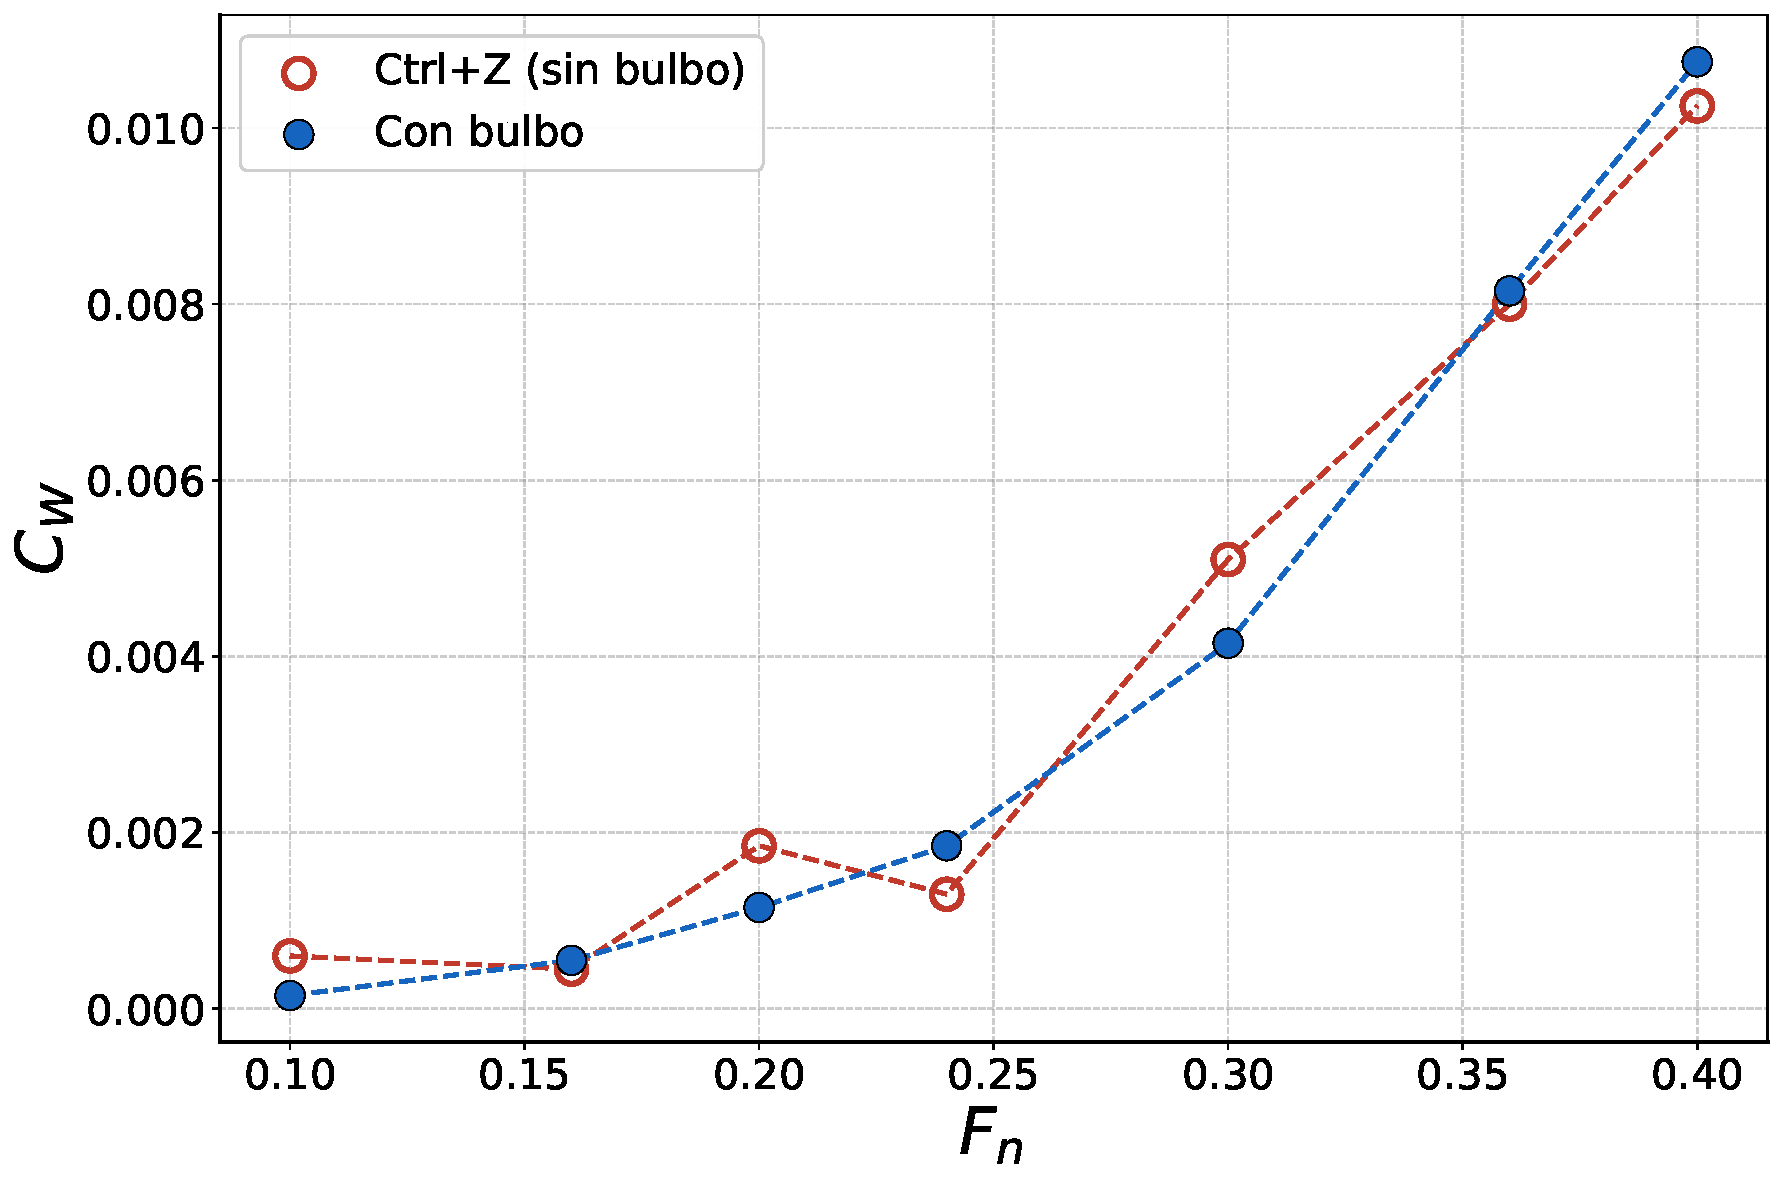
\includegraphics[width=\textwidth]{images/Cw-consinbulbo-195.pdf}
        \caption{Resistencia por olas.}
        \label{fig:Cw_bulbo_195}
    \end{subfigure}

    \vspace{0.6cm}

    \begin{subfigure}[b]{0.48\textwidth}
        \centering
        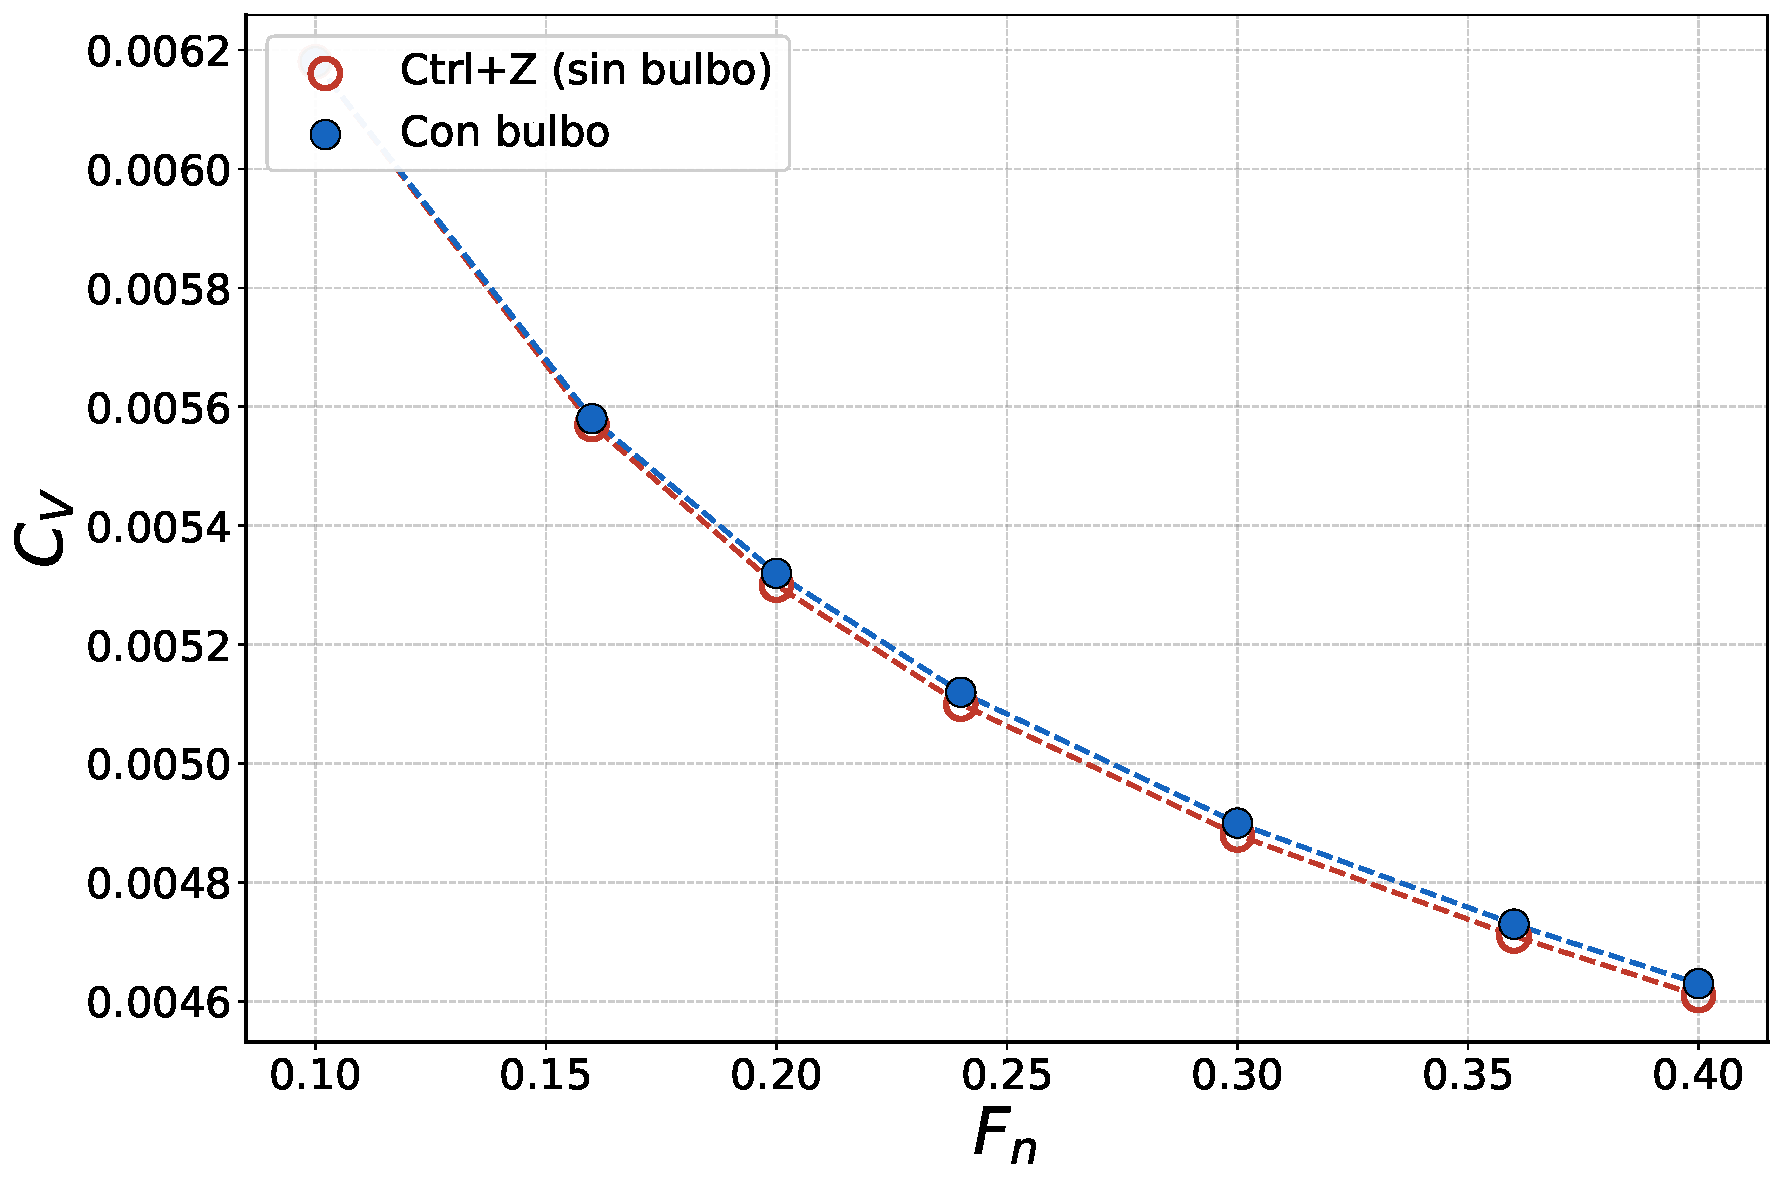
\includegraphics[width=\textwidth]{images/Cv-consinbulbo-195.pdf}
        \caption{Resistencia viscosa. Ambas configuraciones resultan 
        indistinguibles en todo el rango.}
        \label{fig:Cv_bulbo_195}
    \end{subfigure}

    \caption{Descomposición de la resistencia del \textit{P1} con y sin proa 
    bulbo para el calado $T = 0{.}195$~m.}
    \label{fig:coef_bulbo_195}
\end{figure}

Estos resultados, desde el punto de vista hidrodinámico, obligan a repensar 
el diseño de la proa de los pesqueros. Sin embargo, como fue mencionado en 
la introducción, el bulbo ayuda a aumentar la capacidad de carga del buque. 
Aunque su efecto hidrodinámico pueda ser desfavorable según el calado, es 
posible que el análisis económico muestre que la ganancia en capacidad de 
carga supere la pérdida asociada a un diseño no optimizado 
hidrodinámicamente.

\subsection{Efecto sobre el factor de forma}

\paragraph{Efecto sobre el valor de $(1+k)$} La aplicación del método de 
Prohaska a las simulaciones bifásicas de ambas configuraciones arroja los 
valores reunidos en la Tabla~\ref{tab:k_bulbo_ctrlz}. El bulbo incrementa el 
factor de forma en los dos calados analizados, lo cual es consistente con el 
aumento de resistencia por presión viscosa asociado a un cuerpo adicional en 
la proa. La magnitud del efecto, sin embargo, difiere de manera marcada 
entre condiciones de carga: mientras que a $T = 0{.}165$~m el incremento 
alcanza el $3{.}0$\,\%, a $T = 0{.}195$~m se reduce a $0{.}9$\,\%.

\begin{table}[htpb]
\centering
\caption{Factor de forma $(1+k)$ obtenido por el método de Prohaska para 
ambas configuraciones de proa, junto con el rango de $Fr$ empleado en cada 
regresión.}
\label{tab:k_bulbo_ctrlz}
\begin{tabular}{llcc}
\hline
Calado & Configuración & Rango de $Fr$ & $(1+k)$ \\
\hline
\multirow{2}{*}{$T = 0{.}165$~m} & Con bulbo & $0{.}13$--$0{.}20$ & $1{.}204$ \\
                                 & Ctrl+Z    & $0{.}14$--$0{.}20$ & $1{.}169$ \\
\hline
\multirow{2}{*}{$T = 0{.}195$~m} & Con bulbo & $0{.}14$--$0{.}20$ & $1{.}215$ \\
                                 & Ctrl+Z    & $0{.}16$--$0{.}20$ & $1{.}204$ \\
\hline
\end{tabular}
\end{table}

Esta dependencia con el calado resulta coherente con el mecanismo propuesto 
en la literatura: si la contribución del bulbo al factor de forma está 
asociada a su proximidad a la superficie libre, al aumentar el calado el 
bulbo queda más sumergido y su influencia se atenúa. El resultado es 
consistente, además, con el comportamiento de la componente de olas descrito 
en la subsección anterior, donde el beneficio del bulbo también se 
desvanecía al aumentar el calado.

\paragraph{Efecto sobre la tendencia de $(1+k)$ con la velocidad} La 
comparación de las curvas de $(1+k)$ determinadas por doble cuerpo 
(Figuras~\ref{fig:k_bulbo_165} y \ref{fig:k_bulbo_195}) permite abordar la 
segunda de las hipótesis planteadas. Ambas configuraciones presentan un 
crecimiento sostenido de $(1+k)$ con la velocidad, de magnitud comparable, 
sin alcanzar un valor asintótico en el rango analizado. El bulbo desplaza 
las curvas hacia valores mayores, en línea con lo indicado en la 
Tabla~\ref{tab:k_bulbo_ctrlz}, pero no introduce ni modifica 
sustancialmente la tendencia creciente.

Cabe señalar que la determinación por doble cuerpo del casco con bulbo debe 
interpretarse con cautela en cuanto a sus valores absolutos, dado que la 
condición de simetría impuesta en la frontera superior del dominio puede 
distorsionar el campo de presiones en la zona de proa cuando el bulbo se 
encuentra próximo a dicha frontera, tal como se discutió en la 
Sección~\ref{sec:cfd_ff_antec}. El análisis presentado aquí se apoya, por lo 
tanto, en la comparación de tendencias entre configuraciones y no en el 
nivel absoluto de cada curva.

\begin{figure}[htpb]
    \centering
    \begin{subfigure}[b]{0.48\textwidth}
        \centering
        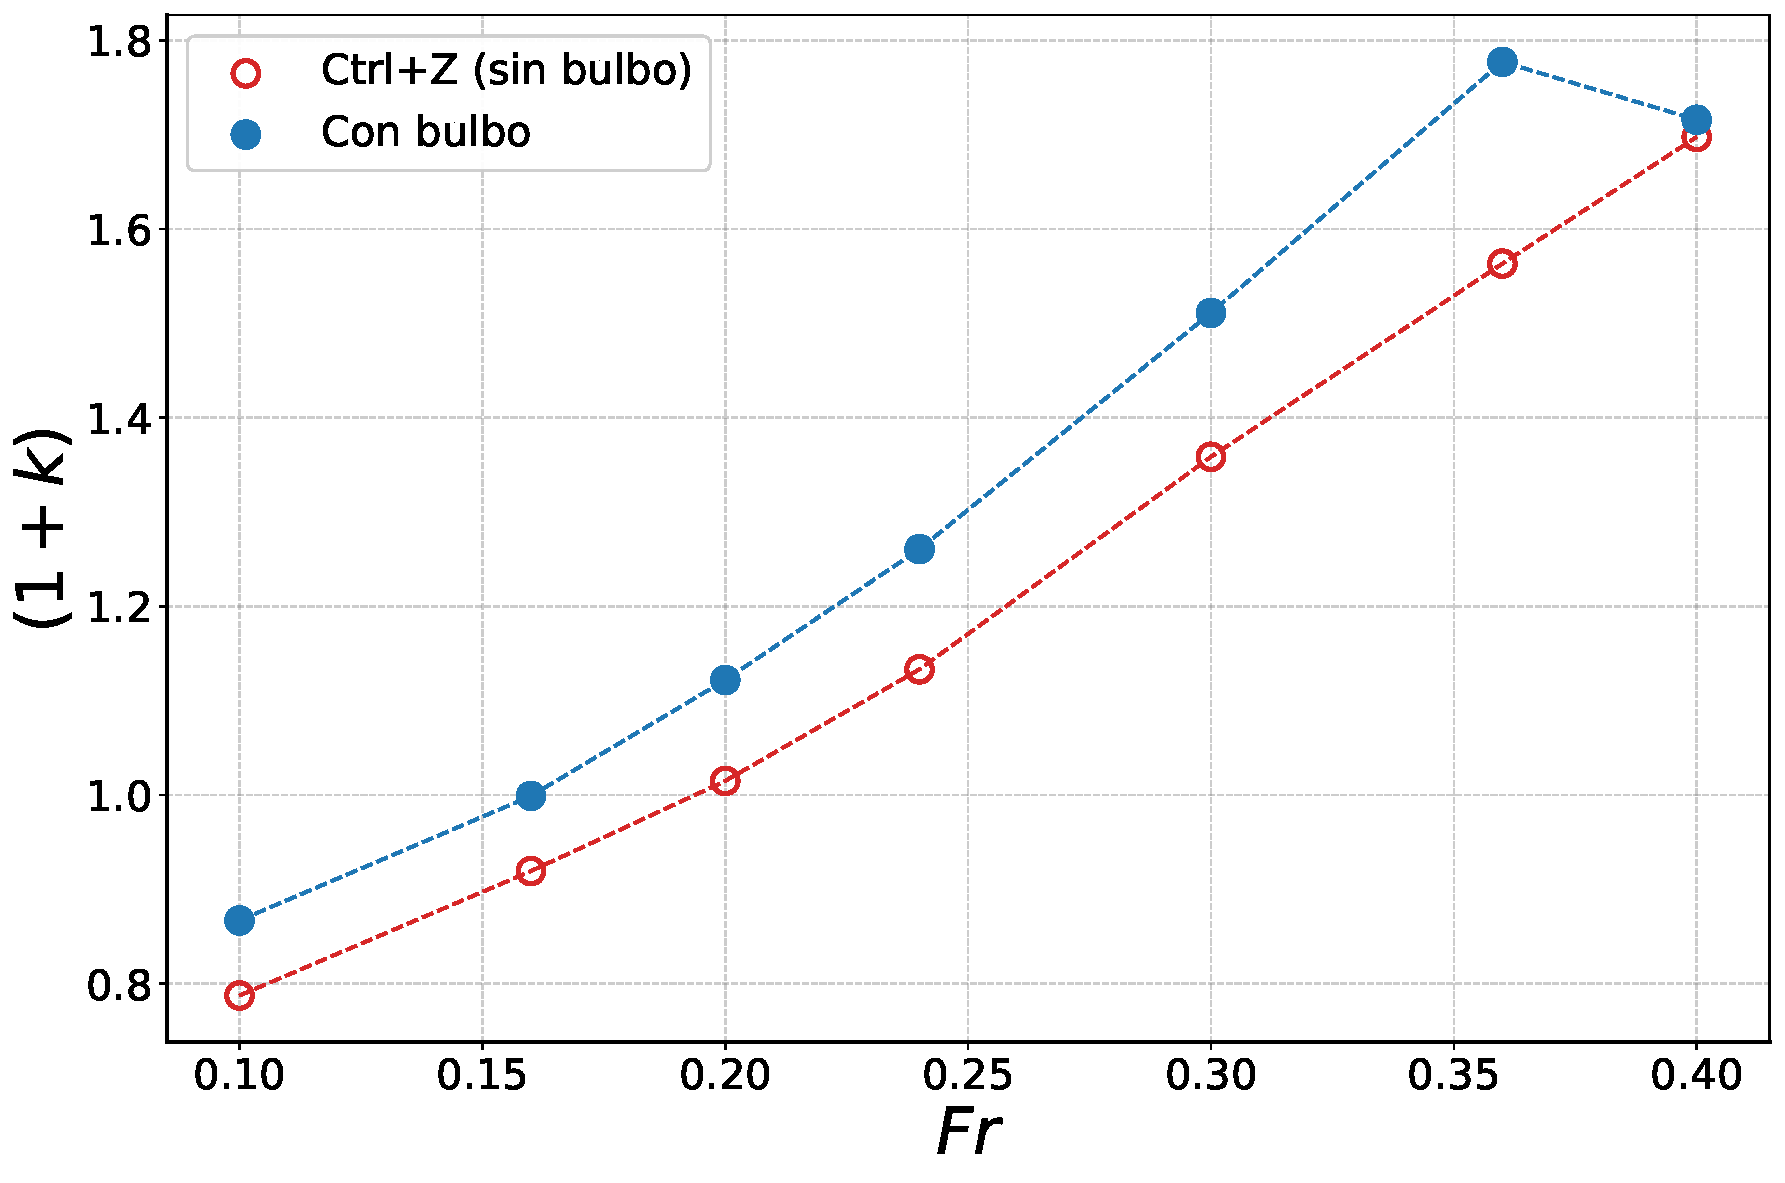
\includegraphics[width=\textwidth]{images/k-consinbulbo-165.pdf}
        \caption{$T = 0{.}165$~m.}
        \label{fig:k_bulbo_165}
    \end{subfigure}
    \hfill
    \begin{subfigure}[b]{0.48\textwidth}
        \centering
        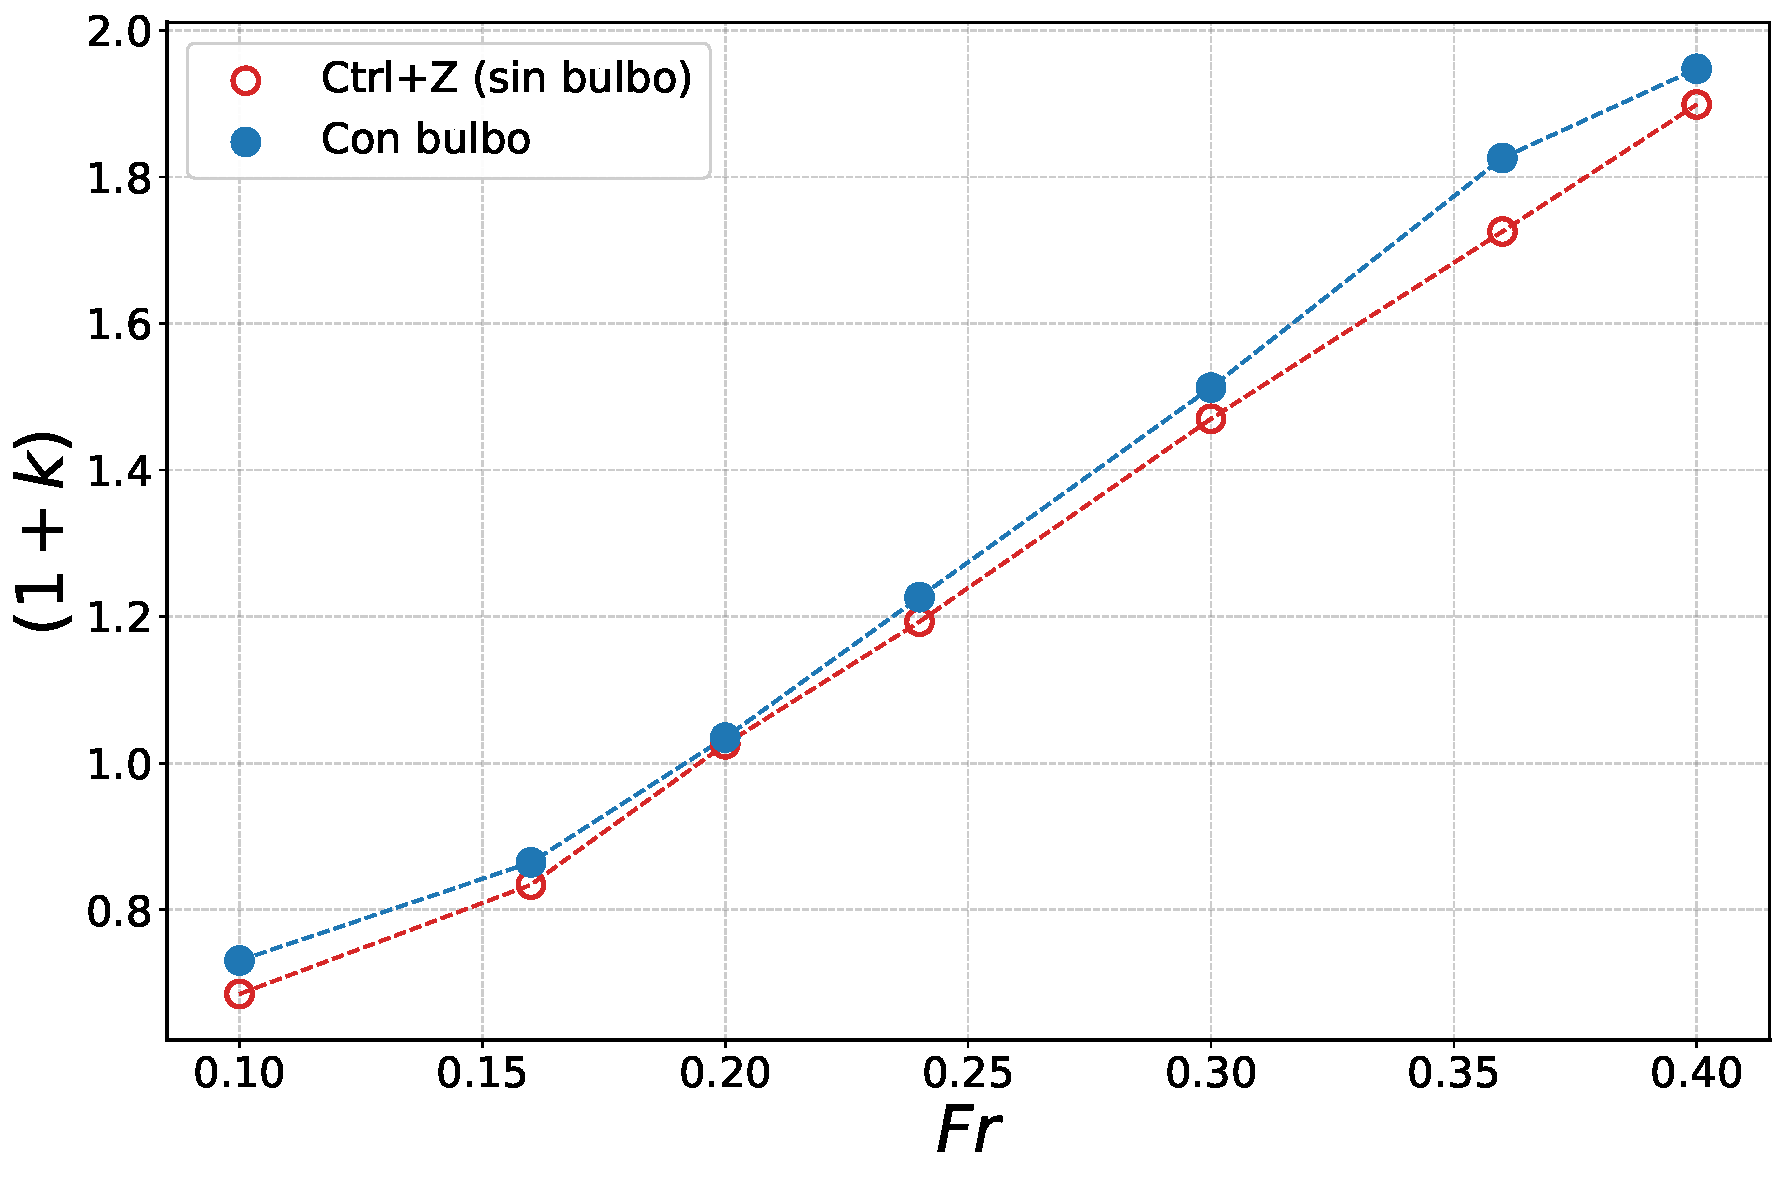
\includegraphics[width=\textwidth]{images/k-consinbulbo-195.pdf}
        \caption{$T = 0{.}195$~m.}
        \label{fig:k_bulbo_195}
    \end{subfigure}

    \caption{Factor de forma $(1+k)$ del \textit{P1} con y sin proa bulbo en 
    función del número de Froude, para ambos calados.}
    \label{fig:k_bulbo}
\end{figure}

\subsection{Conclusiones parciales}

El análisis comparativo entre el \textit{P1} y su variante sin bulbo 
permite extraer tres conclusiones.

En primer lugar, el bulbo modifica el valor del factor de forma determinado 
por el método de Prohaska, incrementándolo en ambos calados, con un efecto 
tres veces mayor en la condición de carga ligera que en la pesada. Esta 
dependencia con el calado es consistente con un mecanismo gobernado por la 
proximidad del bulbo a la superficie libre.

En segundo lugar, el bulbo incrementa la resistencia viscosa y reduce la 
resistencia por olas dentro de su rango de diseño, pero el balance resultante 
depende fuertemente de la condición de carga. A calado reducido resulta 
favorable para la resistencia total por encima de $Fr \approx 0{.}25$, 
mientras que a mayor calado el beneficio desaparece e incluso se invierte en 
el extremo alto del rango de operación.

En tercer lugar, y respecto de la pregunta que motivó este análisis, ni la 
curvatura del diagrama de Prohaska a bajos números de Froude ni la ausencia 
de estabilización de $(1+k)$ con la velocidad pueden atribuirse a la 
presencia del bulbo: ambos comportamientos persisten de manera análoga en el 
modelo Ctrl+Z. Este resultado descarta al bulbo como causa principal y 
refuerza la necesidad de buscar dicha causa en otras características 
geométricas del casco, como su baja relación $L/B$, analizada en la 
Sección~\ref{sec:generalizacion_LB}. Cabe precisar que, en el caso 
particular de la curvatura del diagrama de Prohaska, el análisis aquí 
presentado descarta al bulbo pero no permite distinguir entre un origen 
geométrico y uno numérico asociado al modelado de la transición, dado que 
ambas configuraciones comparten el mismo cierre turbulento.

\section{Influencia de la popa sumergida en el factor de forma}\label{sec:popa_sumergida}

\subsection{Introducción y motivación del estudio}

El estudio de \cite{korkmaz_wetted_transom} analiza la influencia del flujo con \textit{popa mojada} (\textit{wetted-transom flow}) sobre la predicción de la resistencia total y la extrapolación ITTC--78.  
Cuando el espejo de la popa se encuentra sustancialmente sumergido, ya sea por operar a baja velocidad o por calados elevados, se forma una \textbf{zona de recirculación} detrás del espejo, análoga al flujo que ocurre sobre un \textit{backward-facing step} o \textit{escalón hacia atrás}.  
En este régimen, la presión en la arista del espejo no alcanza el valor atmosférico, el flujo se separa y se genera una región de baja presión con un vórtice persistente aguas abajo.

\subsection{Definiciones geométricas y parámetros característicos}

Para describir el grado de inmersión del espejo, \cite{korkmaz_wetted_transom} definió una serie de parámetros adimensionales (Fig.~\ref{fig:transom_defs}), los cuales se expresan mediante las siguientes relaciones:

\begin{equation}
Fr_{tr} = \frac{V}{\sqrt{g\,T_{tr}}}
\end{equation}

\begin{equation}
tr_{\mathrm{ratio}} = \frac{A_{tr}}{A_{\max}}
\end{equation}

\begin{equation}
tr_{\mathrm{fullness}} = \frac{A_{tr}}{2\,y_{tr}\,T_{tr}}
\end{equation}

donde:
\begin{itemize}
  \item $A_{tr}$ es el área del espejo sumergido,
  \item $A_{\max}$ es el área máxima de la sección transversal,
  \item $y_{tr}$ es la mitad de la manga en la intersección del espejo con la superficie libre,
  \item $T_{tr}$ es la inmersión efectiva del borde inferior del espejo,
  \item $T$ el calado total del buque, y
  \item $V$ la velocidad correspondiente a la condición de análisis.
\end{itemize}

El número de Froude del transom $Fr_{tr}$ representa una medida del grado de ``seco o mojado'' del espejo:  
valores bajos indican flujo recirculante (popa mojada), mientras que valores altos ($Fr_{tr} > 3$) corresponden a popas secas o parcialmente mojadas.

\begin{figure}[htpb]
\centering
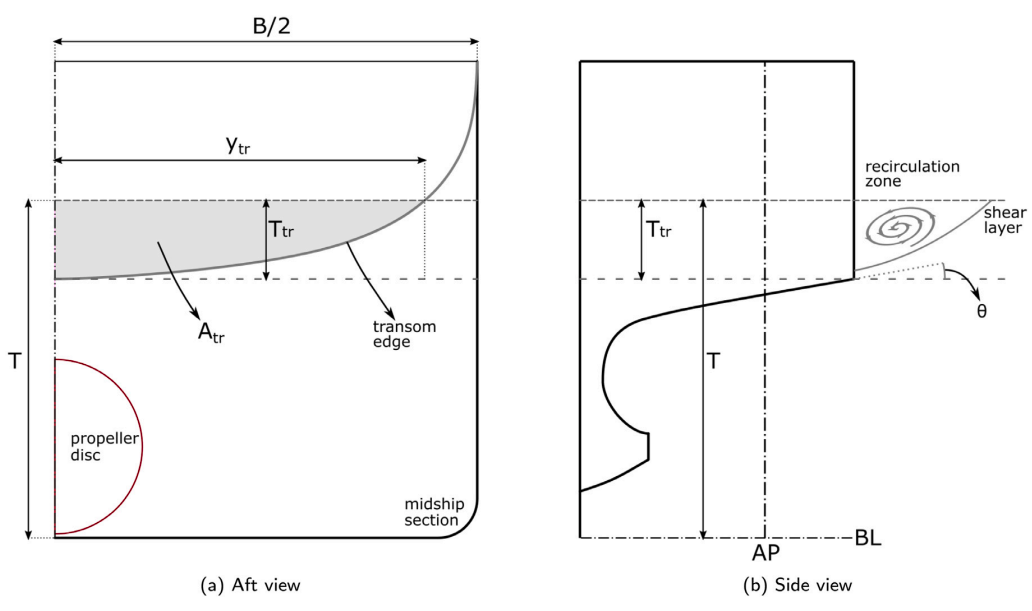
\includegraphics[width=.65\columnwidth]{images/transom_scheme.png}
\caption{Esquema de los parámetros geométricos de popa sumergida, adaptado de \cite{korkmaz_wetted_transom}.}
\label{fig:transom_defs}
\end{figure}

\subsection{Desarrollo del método 2--$k$}

El método \textit{two-form-factor} o 2--$k$ fue propuesto para corregir el déficit de resistencia viscosa generado por la recirculación en popas sumergidas.  
El procedimiento parte de la descomposición clásica de la resistencia viscosa total:

\begin{equation}
C_{V} = (1 + k)\,C_{F0}
\end{equation}

donde $C_{F0}$ es el coeficiente de fricción de ITTC-57 y $(1+k)$ el factor de forma convencional.  
En el caso de popas mojadas, el término $k$ se descompone en dos:

\begin{equation}
k_S = k_M + k_{tr}
\end{equation}

siendo $k_M$ el factor de forma obtenido para el modelo (por método de Prohaska o CFD doble cuerpo), y $k_{tr}$ un incremento asociado al flujo recirculante detrás del espejo, denominado \textit{transom form factor}.  
Este último se expresa como:

\begin{equation}
k_{tr} \simeq \frac{C_{tr,S}}{C_{F,S}}
\end{equation}

donde $C_{tr,S}$ representa la contribución viscosa adicional debida al vórtice de recirculación, y $C_{F,S}$ el coeficiente de fricción a escala buque.

El valor de $k_{tr}$ puede estimarse empíricamente mediante correlaciones con parámetros geométricos del espejo (secciones 6.3 y 7 de \cite{korkmaz_wetted_transom}) o mediante CFD comparativo entre modelo y escala buque:

\begin{equation}
k_{tr} = k_S - k_M
\end{equation}

Este punto es clave, ya que en \citet{korkmaz_wetted_transom} se atribuye la diferencia entre el factor de forma en escala modelo y en escala buque, en los casos de popa espejo sumergida, principalmente al flujo recirculante detrás del espejo. Esta interpretación se enmarca en el trabajo más amplio del mismo autor \citep{korkmaz_cfd_2021, korkmaz_wetted_transom}, donde se demuestra que la dependencia del factor de forma con el número de Reynolds desaparece casi por completo al sustituir la línea ITTC-57 por líneas de fricción numéricas derivadas del mismo código CFD, al menos para cascos de esbeltez moderada como el KCS y el KVLCC2. El efecto de la línea de correlación sobre el \textit{P1} se analiza en la Sección~\ref{sec:linea_de_friccion}. Para cascos de esa clase, donde $C_{PV}$ es comparativamente pequeño, este resultado es consistente con la hipótesis de Hughes: una vez eliminado el sesgo de la línea de referencia, el factor de forma resulta prácticamente independiente de la escala.

De acuerdo con los resultados del autor, el método y las correcciones asociadas deben aplicarse cuando el espejo se encuentra \textbf{considerablemente sumergido}, es decir, para 
$tr_{\mathrm{ratio}} > 0{.}025$. Para espejos poco sumergidos o parcialmente secos, el uso del método 2--$k$ no resulta necesario.

\subsection{Análisis comparativo de flujo}

Antes de aplicar la metodología de \citet{korkmaz_wetted_transom}, es 
necesario verificar que el flujo detrás del espejo sea suficientemente 
similar entre las simulaciones con y sin superficie libre, y que su 
morfología se mantenga estable entre escalas. Ambas condiciones son 
requisitos implícitos del método: la primera asegura que el cálculo de doble 
cuerpo captura adecuadamente la resistencia asociada a la recirculación, y la 
segunda justifica la aplicación de un $k_{tr}$ constante entre modelo y 
buque.

Los resultados de las simulaciones con superficie libre, presentados en la 
Figura~\ref{fig:recirculacion_comparativa1}, muestran que la estructura del 
flujo en la zona de popa se mantiene estable entre escalas para $Fr = 0{.}16$ 
y $Fr = 0{.}36$: no se registran desprendimientos nuevos ni variaciones 
morfológicas significativas en el núcleo de recirculación al pasar de escala 
modelo a escala buque.

\begin{figure}[htpb]
    \centering
    \begin{subfigure}{0.48\textwidth}
        \centering
        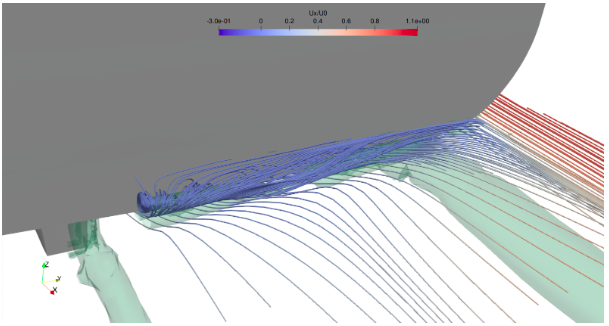
\includegraphics[width=\linewidth]{images/195-016-consup-modelo.png}
        \caption{Escala modelo, $Fr = 0{.}16$}
    \end{subfigure}
    \hfill
    \begin{subfigure}{0.48\textwidth}
        \centering
        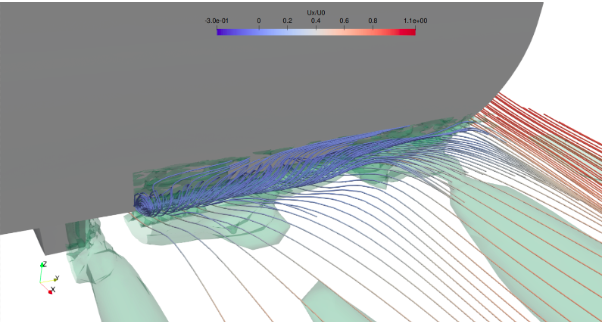
\includegraphics[width=\linewidth]{images/195-016-consup-real.png}
        \caption{Escala buque, $Fr = 0{.}16$}
    \end{subfigure}

    \vspace{0.5cm}

    \begin{subfigure}{0.48\textwidth}
        \centering
        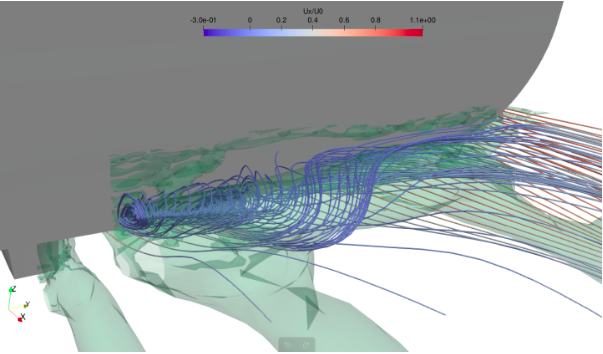
\includegraphics[width=\linewidth]{images/195-036-consup-modelo.png}
        \caption{Escala modelo, $Fr = 0{.}36$}
    \end{subfigure}
    \hfill
    \begin{subfigure}{0.48\textwidth}
        \centering
        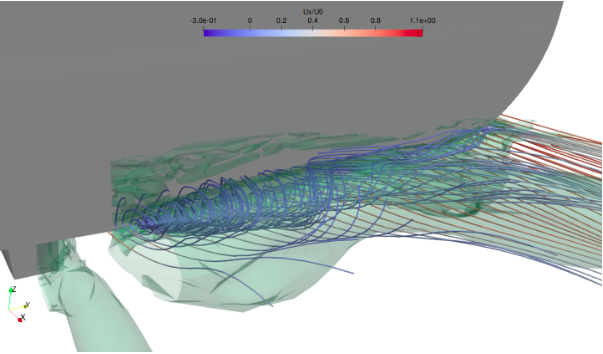
\includegraphics[width=\linewidth]{images/195-036-consup-real.png}
        \caption{Escala buque, $Fr = 0{.}36$}
    \end{subfigure}

    \caption{Comparación de la recirculación en popa sumergida para distintas 
    escalas y números de Froude (calado 0{.}195~m). Casos con superficie libre.}
    \label{fig:recirculacion_comparativa1}
\end{figure}

De manera análoga, en los casos de cuerpo doble ilustrados en la Figura~\ref{fig:recirculacion_comparativa2}, la estructura de recirculación es igualmente estable en todo el rango de velocidades y escalas analizadas. La similitud entre los resultados con y sin superficie libre, tanto a escala 
modelo como a escala buque, confirma que la hipótesis de doble cuerpo captura adecuadamente la física del flujo en la zona de popa para este casco. La persistencia de la recirculación al aumentar $Re$ es precisamente la 
condición que, según \citet{korkmaz_wetted_transom}, origina el déficit de resistencia viscosa en la extrapolación estándar y que motiva la aplicación del método 2--$k$.

\begin{figure}[htpb]
    \centering
    \begin{subfigure}{0.48\textwidth}
        \centering
        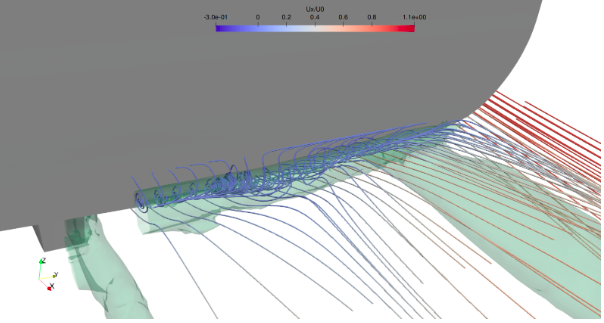
\includegraphics[width=\linewidth]{images/195-016-sinsup-modelo.png}
        \caption{Escala modelo, $Fr = 0{.}16$}
    \end{subfigure}
    \hfill
    \begin{subfigure}{0.48\textwidth}
        \centering
        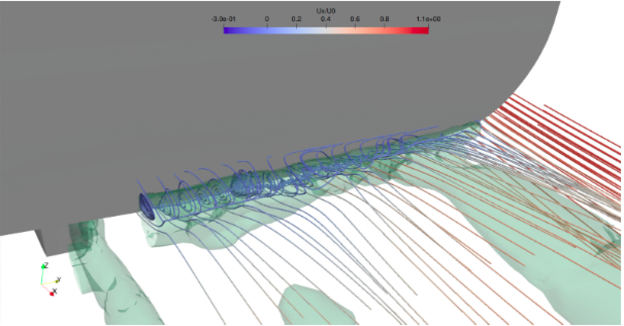
\includegraphics[width=\linewidth]{images/195-016-sinsup-real.png}
        \caption{Escala buque, $Fr = 0{.}16$}
    \end{subfigure}

    \vspace{0.5cm}

    \begin{subfigure}{0.48\textwidth}
        \centering
        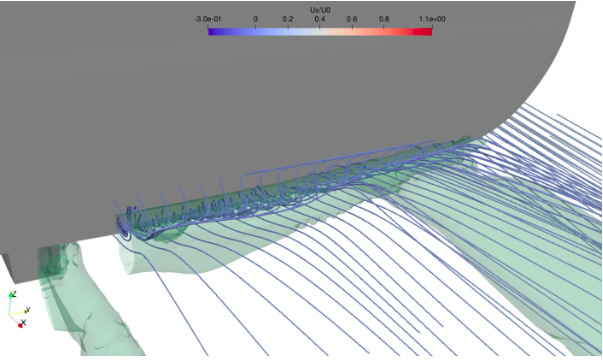
\includegraphics[width=\linewidth]{images/195-036-sinsup-modelo.png}
        \caption{Escala modelo, $Fr = 0{.}36$}
    \end{subfigure}
    \hfill
    \begin{subfigure}{0.48\textwidth}
        \centering
        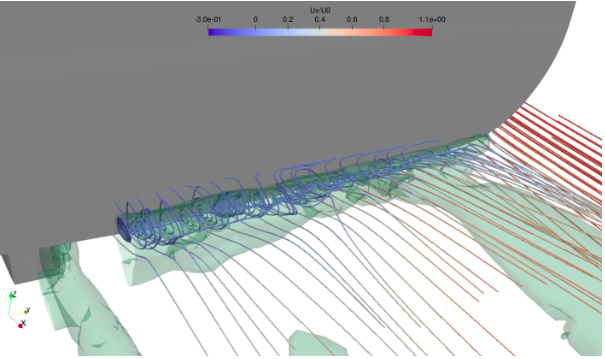
\includegraphics[width=\linewidth]{images/195-036-sinsup-real.png}
        \caption{Escala buque, $Fr = 0{.}36$}
    \end{subfigure}

    \caption{Comparación de la recirculación en popa sumergida para distintas 
    escalas y números de Froude (calado 0{.}195~m). Casos sin superficie libre.}
    \label{fig:recirculacion_comparativa2}
\end{figure}

\subsection{Aplicación al Pesquero~1}

La geometría de popa del Pesquero~1 presenta una inmersión del espejo que, según los criterios establecidos por \citet{korkmaz_wetted_transom}, debe evaluarse en condición estática ($Fr = 0$), ya que el método demanda los parámetros geométricos correspondientes al buque en reposo. La Tabla~\ref{tab:tpa_transom_params} resume los parámetros calculados para esa condición.

\begin{table}[h]
\centering
\caption{Parámetros de popa sumergida del \textit{P1} en condición estática 
($Fr = 0$, calado $T = 0{.}195$~m).}
\label{tab:tpa_transom_params}
\small
\begin{tabular}{lc}
\toprule
\textbf{Parámetro} & \textbf{Valor} \\
\midrule
$A_{tr}$ [m$^2$]            & 0{.}00222 \\
$A_{\max}$ [m$^2$]          & 0{.}04 \\
$y_{tr}$ [m]                & 0{.}198 \\
$T_{tr}$ [m]                & 0{.}0164 \\
$T$ [m]                     & 0{.}195 \\
\addlinespace[3pt]
$tr_{\text{ratio}}$         & 0{.}056 \\
$tr_{\text{fullness}}$      & 0{.}342 \\
\addlinespace[3pt]
$k_{tr}$                    & 0{.}025 \\
\bottomrule
\end{tabular}
\end{table}

El valor de $tr_{\text{ratio}} = 0{.}056$ supera el umbral de $0{.}025$ 
establecido por \citet{korkmaz_wetted_transom}, por lo que corresponde aplicar 
la corrección. El factor de forma de escala buque queda entonces:

\begin{equation}
    k_S = k_M + k_{tr} = 0{.}194 + 0{.}025 = 0{.}219
    \quad \Rightarrow \quad
    (1+k_S) = 1{.}219
\end{equation}

Sin embargo, para evaluar si este mecanismo explica la diferencia observada 
entre escalas, es necesario compararlo con la magnitud total de esa diferencia. 
Según los resultados de CFD DB presentados en la 
Sección~\ref{sec:analisis_efectos_escala}, el valor de $(1+k)$ a escala buque 
es de aproximadamente $1{.}716$ ($k_S = 0{.}716$), mientras que el valor adoptado 
a escala modelo es $(1+k_M) = 1{.}194$ ($k_M = 0{.}194$). La diferencia total es:

\begin{equation}
    k_S - k_M = 0{.}716 - 0{.}194 = 0{.}522
\end{equation}

La corrección de popa mojada $k_{tr} = 0{.}025$ representa apenas el $5\%$ de 
esa diferencia. El método 2--$k$ de \citet{korkmaz_wetted_transom} fue 
desarrollado para cascos donde la recirculación de popa espejo es el 
mecanismo dominante del efecto de escala en el factor de forma; en el 
\textit{P1}, en cambio, la diferencia entre escalas está gobernada por la 
evolución de $C_{PV}$ asociada a las estructuras vorticosas de quilla y 
pantoque, cuya intensidad se mantiene estable con $Re$, como se demostró en 
la Sección~\ref{sec:descomposicion_de_la_res_viscosa}. La recirculación de 
popa espejo contribuye a ese efecto de escala total, pero con un peso 
marginal.

\subsection{Conclusiones parciales}

El análisis comparativo de flujo confirma que la estructura de recirculación en la zona del espejo de popa se mantiene estable frente al cambio de escala, tanto en las simulaciones con superficie libre como en las de doble cuerpo. 
Esta persistencia de la recirculación con $Re$ es precisamente la condición que, según \citet{korkmaz_wetted_transom}, origina un déficit de resistencia viscosa en la extrapolación estándar y que justifica la aplicación del método 2--$k$.

La aplicación del método al \textit{P1} arroja $k_{tr} = 0{.}025$, lo que representa aproximadamente el $5\%$ de la diferencia total observada entre el factor de forma a escala modelo y a escala buque ($k_S - k_M = 0{.}522$). 
Este resultado permite cuantificar la contribución de la popa espejo sumergida al efecto de escala total y, al mismo tiempo, descartarla como causa principal: la diferencia predominante tiene su origen en la evolución de $C_{PV}$ asociada a las estructuras vorticosas de quilla y pantoque, cuyo mecanismo fue analizado en la Sección~\ref{sec:descomposicion_de_la_res_viscosa}. 
El análisis del efecto de la línea de fricción, que completa el diagnóstico de los efectos de escala en el \textit{P1}, se presenta en la Sección~\ref{sec:linea_de_friccion}.

\section{Efecto de la línea de fricción}\label{sec:linea_de_friccion}

Como se discutió en la Sección~\ref{sec:ITTC57}, el uso de la línea de 
correlación ITTC-57 introduce una dependencia artificial del factor de forma 
con el número de Reynolds que desaparece casi por completo al sustituirla 
por líneas de fricción numéricas (NFL), al menos para cascos de esbeltez 
moderada. En esta sección se evalúa si este efecto es suficiente para 
explicar la variación de $(1+k)$ con $Re$ observada en el \textit{P1}.

La Figura~\ref{ittc_nfl} presenta la variación de $(1+k)$ frente al número 
de Reynolds para el \textit{P1}, considerando la línea ITTC-57 
\citep{ITTC_resistance} y la NFL propuesta por \citet{Korkmaz2019NumericalFL}.

\begin{figure}[htpb]
	\centering
	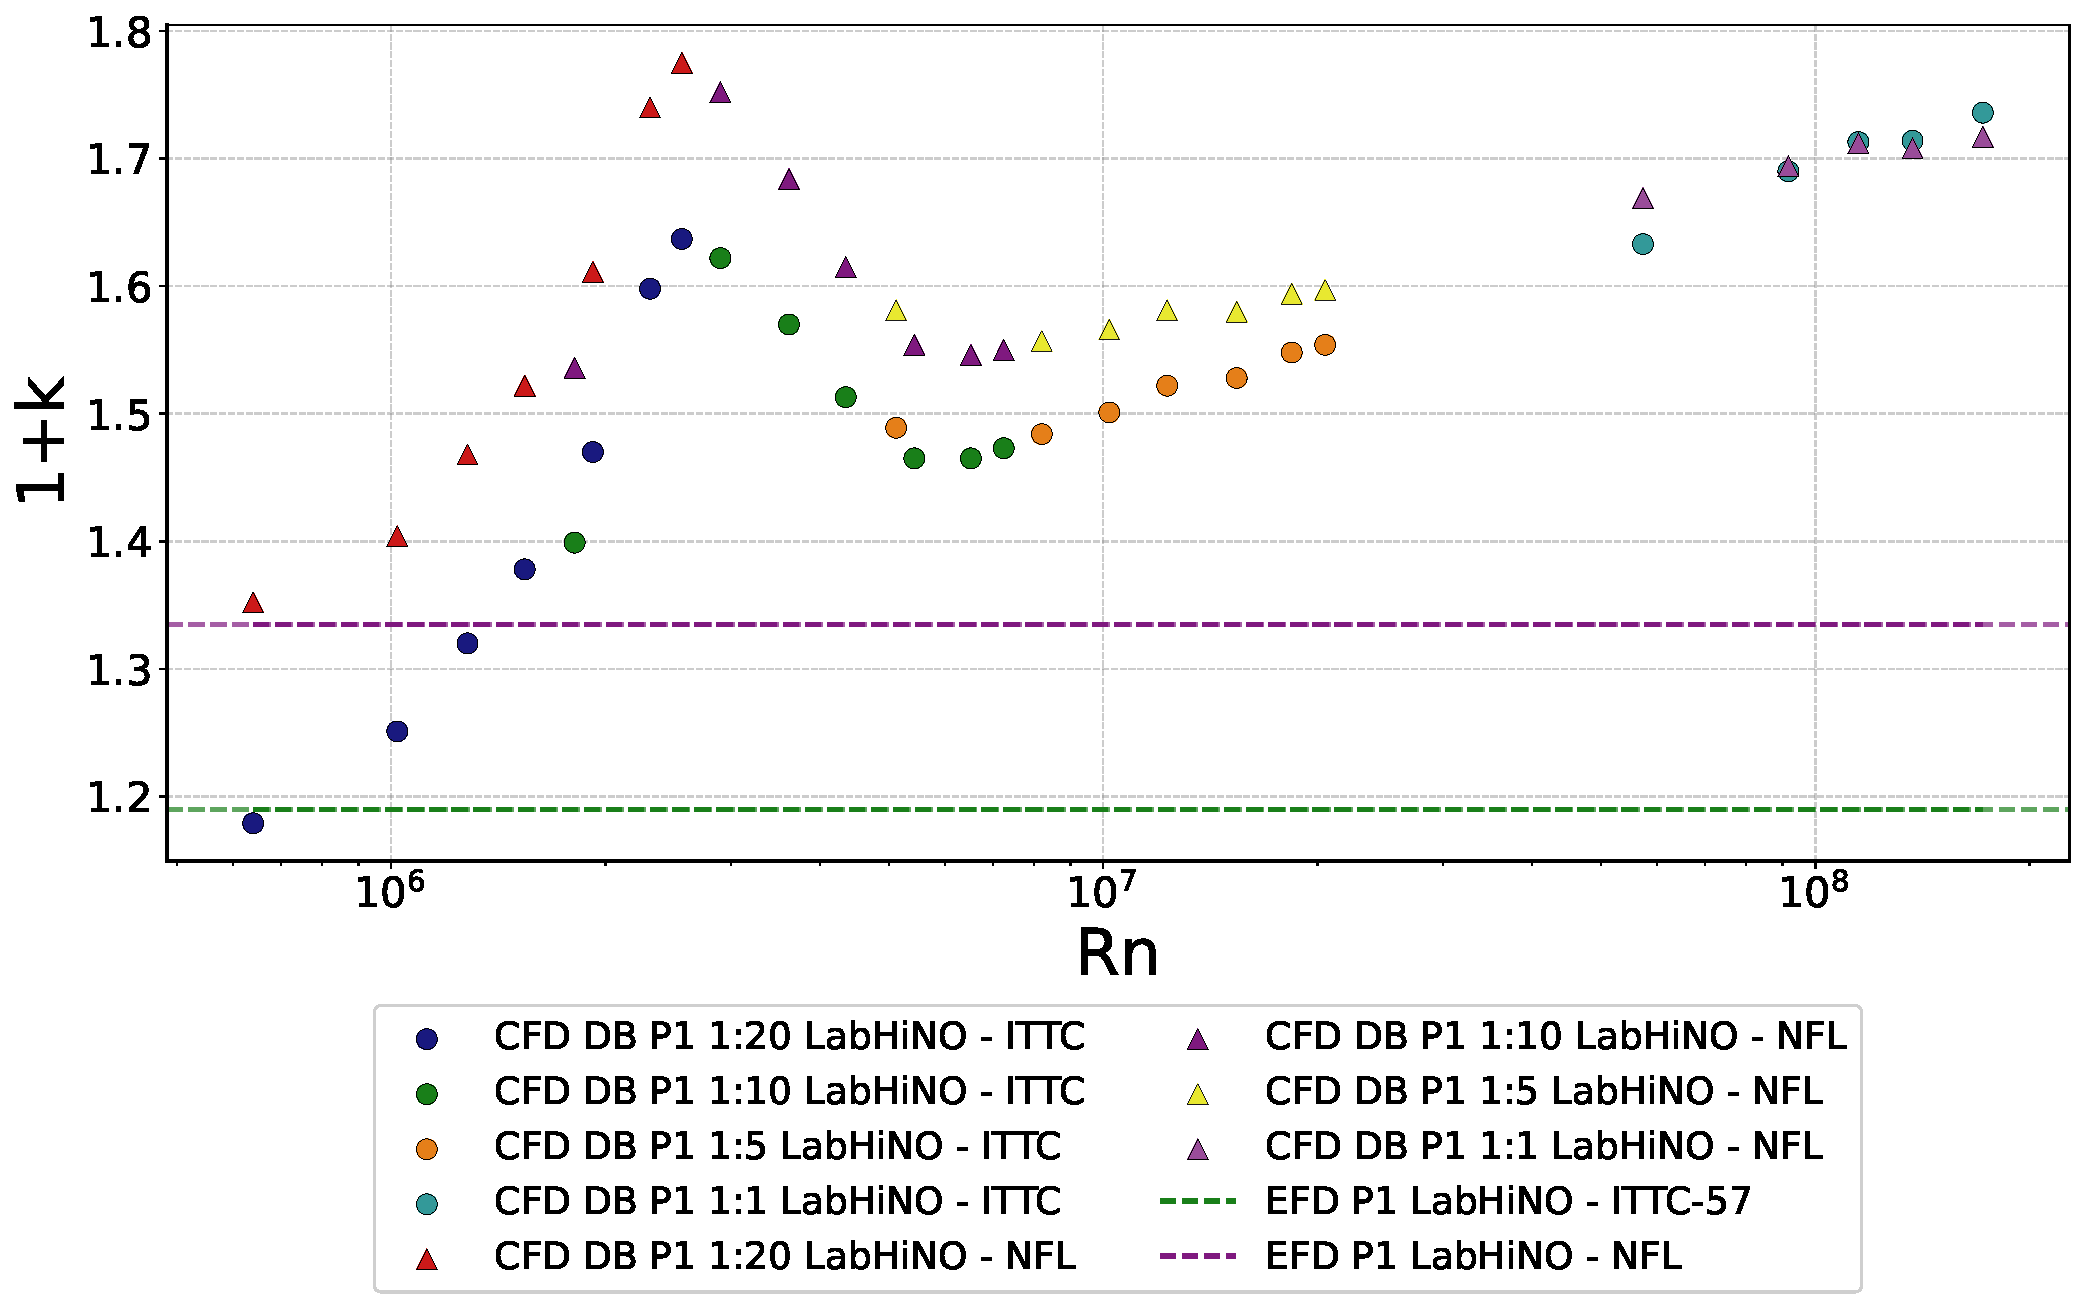
\includegraphics[width=.6\columnwidth]{images/ittc-nfl.pdf}
	\caption{Variación de $(1+k)$ en función de $Re$ para el \textit{P1} 
	empleando la línea ITTC-57 y la NFL de \citet{Korkmaz2019NumericalFL}.}
	\label{ittc_nfl}
\end{figure}

Al emplear la NFL, se observan valores de $(1+k)$ ligeramente más altos a 
bajos $Re$ y, en consecuencia, una variación total algo menor del factor de 
forma a lo largo del rango de escalas. Sin embargo, la diferencia entre el 
valor de $(1+k)$ a bajo y alto $Re$ continúa siendo considerable, del orden 
del 25\%, frente al 40\% obtenido con la ITTC-57. Para altos números de 
Reynolds (escala buque), el valor de $(1+k)$ resulta prácticamente idéntico 
independientemente de la línea de fricción utilizada, como cabría esperar 
dado que las diferencias entre formulaciones se concentran en el régimen de 
bajo $Re$.

En síntesis, la sustitución de la línea ITTC-57 por una NFL reduce 
parcialmente la variación de $(1+k)$ con $Re$, pero no la elimina: la 
diferencia entre escalas continúa siendo sustancial. Esto confirma que el 
efecto de escala en el \textit{P1} no puede atribuirse exclusivamente al 
sesgo de la línea de correlación, sino que responde principalmente a la 
física del flujo, en particular a la evolución de $C_{PV}$ con $Re$ 
asociada a las estructuras vorticosas de popa, como se analizó en la 
Sección~\ref{sec:descomposicion_de_la_res_viscosa}.

\section{Efecto de los modelos de turbulencia}

\subsection{Introducción y motivación del estudio}

El modelado de la turbulencia constituye una de las principales fuentes de 
incertidumbre en la simulación numérica de la resistencia viscosa. Los modelos 
basados en las ecuaciones de Navier--Stokes promediadas por Reynolds (RANS) 
introducen un cierre empírico a través de la denominada \textit{viscosidad 
turbulenta}, cuyo valor depende del modelo de turbulencia seleccionado. Dado 
que la estimación del factor de forma $(1+k)$ se basa en la partición entre 
resistencia friccional y de presión viscosa, cualquier variación en la 
predicción del campo de velocidades o en la distribución de esfuerzos de corte 
puede modificar significativamente el resultado final.

En esta sección se analiza la influencia del modelo de turbulencia sobre la 
determinación numérica del factor de forma, comparando cuatro formulaciones 
ampliamente utilizadas en hidrodinámica naval: $k$--$\omega$, $k$--$\omega$ SST, 
$k$--$\varepsilon$ estándar y $k$--$\varepsilon$ realizable. El objetivo es 
evaluar su sensibilidad en la estimación de $C_F$, $C_{PV}$ y $(1+k)$ para el 
caso del \textit{P1}, y verificar la consistencia de las predicciones frente al 
valor experimental obtenido mediante el método de Prohaska.

\subsection{Metodología y configuración numérica}

Las simulaciones se realizaron bajo las mismas condiciones numéricas y de 
contorno descritas en la Sección~\ref{sec:doble_cuerpo}: dominio de cuerpo 
doble sin superficie libre, flujo estacionario y configuración de malla 
equivalente. Las únicas variaciones entre casos corresponden al modelo de 
turbulencia empleado, de modo que las diferencias observadas sean atribuibles 
exclusivamente al cierre turbulento.

\subsection{Modelos de turbulencia analizados}

A continuación se presenta la formulación y las diferencias conceptuales entre 
los modelos de turbulencia empleados para el análisis de sensibilidad. El 
objetivo es contrastar el modelo $k$--$\omega$ SST, utilizado en todos los 
cálculos presentados hasta ahora, con formulaciones alternativas para evaluar 
su impacto en la predicción de la resistencia viscosa y el factor de forma 
$(1+k)$.

\paragraph{Modelo $k$--$\omega$ SST}

El modelo $k$--$\omega$ SST (\textit{Shear Stress Transport}) fue utilizado 
como modelo de referencia para todos los cálculos presentados en los capítulos 
anteriores. Su formulación detallada y la justificación de su elección se 
encuentran descritas en la Sección~\ref{sec:metodo_SST} del 
Capítulo~\ref{chap:Metodologia}. En esta comparativa, sus resultados sirven 
como línea de referencia frente a la cual se evalúan las desviaciones de los 
otros modelos.

\paragraph{Modelo $k$--$\omega$ estándar}

El modelo $k$--$\omega$ original \citep{Wilcox1988} es un modelo RANS de dos 
ecuaciones que resuelve la energía cinética turbulenta $k$ y la tasa 
específica de disipación $\omega$. Las ecuaciones de transporte se escriben 
como:

\begin{equation}
\frac{\partial k}{\partial t} + U_j \frac{\partial k}{\partial x_j}
=
P_k - \beta^* k \omega
+ \frac{\partial}{\partial x_j}
\left[
(\nu + \sigma_k \nu_t)\frac{\partial k}{\partial x_j}
\right],
\end{equation}

\begin{equation}
\frac{\partial \omega}{\partial t} + U_j \frac{\partial \omega}{\partial x_j}
=
\alpha \frac{\omega}{k} P_k - \beta \omega^2
+ \frac{\partial}{\partial x_j}
\left[
(\nu + \sigma_\omega \nu_t)\frac{\partial \omega}{\partial x_j}
\right],
\end{equation}

donde $U_j$ es la velocidad, $P_k$ es el término de producción de energía 
cinética turbulenta, $\nu$ es la viscosidad cinemática molecular, $\nu_t$ es la viscosidad cinemática turbulenta, y $\beta^*$, $\beta$, $\alpha$, 
$\sigma_k$ y $\sigma_\omega$ son constantes del modelo.

La viscosidad turbulenta se define como:

\begin{equation}
\nu_t = \frac{k}{\omega}.
\end{equation}

Aunque este modelo presenta una buena resolución de la capa límite viscosa 
sin necesidad de funciones de amortiguamiento, es conocido por su fuerte 
sensibilidad a las condiciones de contorno de turbulencia en el flujo libre 
(\textit{freestream sensitivity}), lo que puede afectar la predicción del 
campo turbulento global si el dominio no es suficientemente grande.

\paragraph{Modelo $k$--$\varepsilon$ estándar}

El modelo $k$--$\varepsilon$ estándar \citep{Launder1974} resuelve las 
ecuaciones de transporte para la energía cinética turbulenta $k$ y su tasa 
de disipación $\varepsilon$:

\begin{equation}
\frac{\partial k}{\partial t} + U_j \frac{\partial k}{\partial x_j}
=
P_k - \varepsilon
+ \frac{\partial}{\partial x_j}
\left[
(\nu + \sigma_k \nu_t)\frac{\partial k}{\partial x_j}
\right],
\end{equation}

\begin{equation}
\frac{\partial \varepsilon}{\partial t} + U_j \frac{\partial \varepsilon}{\partial x_j}
=
C_{\varepsilon 1} \frac{\varepsilon}{k} P_k
- C_{\varepsilon 2} \frac{\varepsilon^2}{k}
+ \frac{\partial}{\partial x_j}
\left[
(\nu + \sigma_\varepsilon \nu_t)\frac{\partial \varepsilon}{\partial x_j}
\right],
\end{equation}

donde $C_{\varepsilon 1}$, $C_{\varepsilon 2}$ y $\sigma_\varepsilon$ son 
constantes del modelo. La viscosidad turbulenta se define como:

\begin{equation}
\nu_t = C_\mu \frac{k^2}{\varepsilon},
\end{equation}

con $C_\mu$ constante. Este modelo asume equilibrio local entre producción y 
disipación y fue calibrado para flujos completamente turbulentos y alejados 
de la pared. Como consecuencia, tiende a sobreestimar la difusión turbulenta 
en la capa límite y no resulta adecuado para capturar con precisión efectos 
de separación bajo gradientes de presión adversos, tendiendo a predecir una 
re-adhesión del flujo demasiado temprana en la popa.

\paragraph{Modelo $k$--$\varepsilon$ realizable}

El modelo $k$--$\varepsilon$ realizable \citep{Shih1994} introduce 
modificaciones conceptuales al modelo estándar con el objetivo de cumplir 
restricciones matemáticas sobre los esfuerzos de Reynolds 
(\textit{realizability}), evitando la generación de energía cinética negativa 
en flujos con grandes deformaciones medias. En particular, el coeficiente 
$C_\mu$ deja de ser constante y pasa a depender del estado local del flujo 
(tasa de deformación y rotación), y la ecuación de $\varepsilon$ se 
reformula para mejorar la predicción de flujos con rotación, separación 
moderada y estelas:

\begin{equation}
\nu_t = C_\mu(\mathbf{U}, \nabla \mathbf{U}) \frac{k^2}{\varepsilon},
\end{equation}

donde $\mathbf{U}$ es el vector de velocidades medias y $\nabla \mathbf{U}$ 
su gradiente. Estas modificaciones permiten reducir la difusión excesiva 
característica del modelo estándar y mejorar la predicción de estructuras 
vorticosas coherentes. Se incluye en este análisis para evaluar si una 
formulación $k$--$\varepsilon$ mejorada puede acercarse a los resultados del 
modelo $k$--$\omega$ SST para la determinación del factor de forma.

\subsection{Comparación de resistencia viscosa}

La Figura~\ref{fig:comparacion_cd} presenta los coeficientes de resistencia 
viscosa total $C_V$ obtenidos para los cuatro modelos de turbulencia en 
función del número de Reynolds. A bajo $Re$, donde el flujo se encuentra en 
régimen transicional, se observa una dispersión significativa entre modelos.

Entre los modelos evaluados, el $k$--$\omega$ SST predice los valores más 
bajos de $C_V$, mientras que el $k$--$\varepsilon$ estándar predice los 
valores más altos. El modelo $k$--$\varepsilon$ realizable reduce parcialmente 
esta discrepancia, situándose entre ambos. Este comportamiento coincide con 
lo reportado por \citet{Karim}, quien observó una secuencia análoga en la 
predicción de la resistencia de cuerpos sumergidos a $Re = 2\times10^7$: la 
mayor concordancia con los datos experimentales correspondió al $k$--$\omega$ 
SST, seguido del $k$--$\varepsilon$ realizable, el $k$--$\varepsilon$ estándar 
y finalmente el $k$--$\omega$.

A medida que $Re$ aumenta, las diferencias entre modelos disminuyen y todos 
convergen hacia una tendencia común. Esto sugiere que las discrepancias son 
dominantes solo en el rango transicional, donde la fracción de flujo laminar 
o la intensidad del campo de recirculación varían según el modelo.

\begin{figure}[htpb]
    \centering
    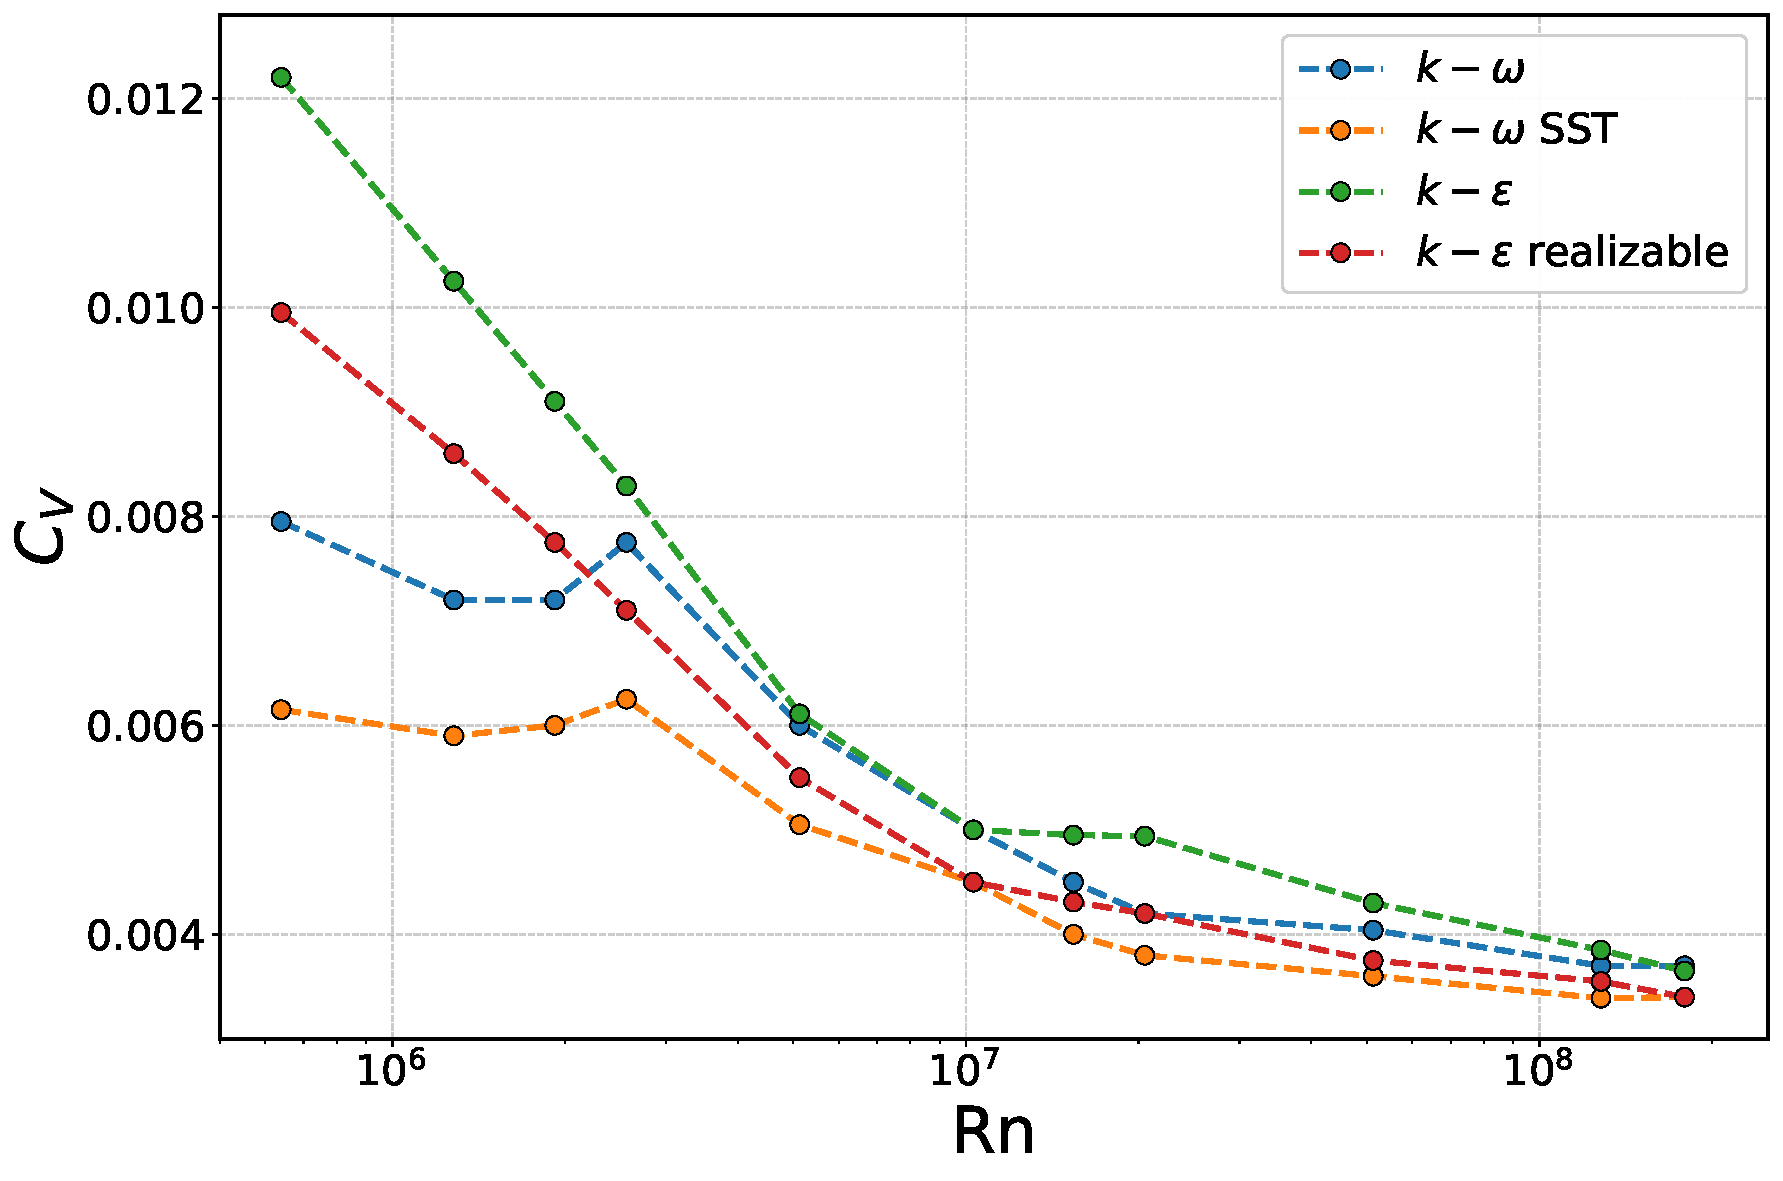
\includegraphics[width=0.75\textwidth]{images/comparacion_ct.pdf}
    \caption{Comparación de $C_V$ obtenido mediante distintos modelos de 
    turbulencia para el \textit{P1}.}
    \label{fig:comparacion_cd}
\end{figure}

\subsection{Efecto sobre el factor de forma}

La Figura~\ref{fig:comparacion_k} muestra la evolución del factor de forma 
$(1+k)$ con el número de Reynolds para los cuatro modelos. El $k$--$\omega$ 
SST presenta la mayor concordancia con el valor experimental del 
\textit{P1} ($1+k \approx 1.30$ en $Re \approx 10^6$). El modelo 
$k$--$\omega$ predice valores más altos de $(1+k)$ que el $k$--$\omega$ SST 
en el rango intermedio ($Re \approx 2\times10^7$), atribuibles al incremento 
de la resistencia de presión viscosa observada en ese régimen. En cambio, el 
$k$--$\varepsilon$ estándar y el $k$--$\varepsilon$ realizable exhiben 
pendientes más suaves y tienden a converger hacia valores similares a los del 
$k$--$\omega$ SST a alto $Re$.

\begin{figure}[htpb]
    \centering
    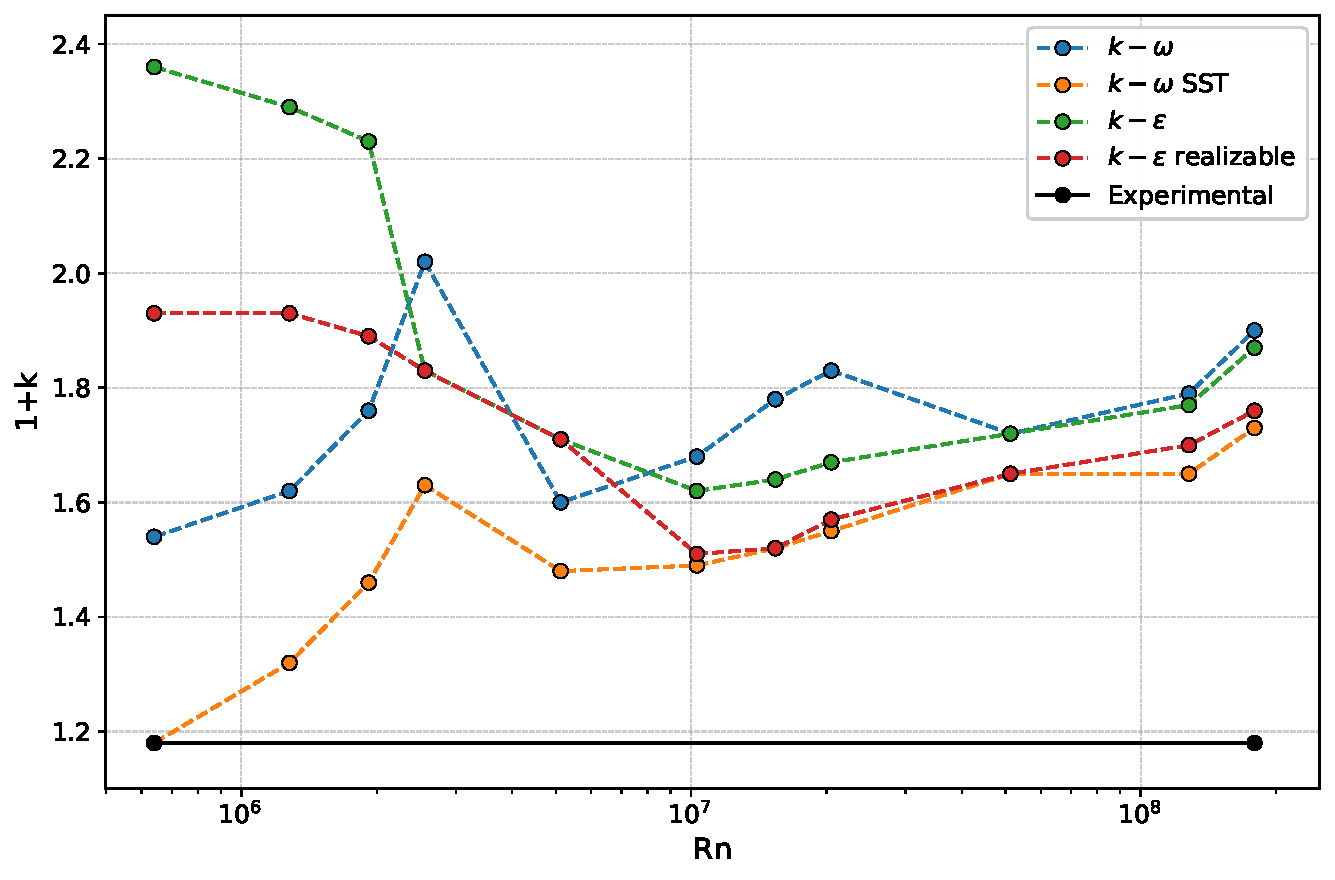
\includegraphics[width=0.75\textwidth]{images/comparacion_k.pdf}
    \caption{Evolución del factor de forma $(1+k)$ en función de $Re$ para 
    distintos modelos de turbulencia. \textit{P1}.}
    \label{fig:comparacion_k}
\end{figure}

Este resultado pone de manifiesto que la elección del modelo de turbulencia 
afecta principalmente el comportamiento del factor de forma a bajo y mediano 
$Re$, donde el flujo puede contener zonas parcialmente laminares o 
recirculaciones locales en popa. A alto $Re$, donde el flujo es plenamente 
turbulento y las capas límite están bien desarrolladas, la sensibilidad del 
cálculo a la elección del modelo disminuye marcadamente.

\subsection{Descomposición de la resistencia según origen friccional y 
de presión viscosa}

Para profundizar en las causas de las diferencias anteriores, las 
Figuras~\ref{fig:comparacion_cf} y \ref{fig:comparacion_cp} muestran la 
variación del coeficiente de fricción $C_F$ y del coeficiente de presión 
viscosa $C_{PV}$ con $Re$. En la primera se aprecia que $k$--$\omega$ SST 
reproduce la correlación ITTC-57 en casi todo el rango de $Re$, salvo en la 
zona más baja donde el flujo se encuentra parcialmente transicional. Por su 
parte, el $k$--$\omega$ tiende a sobreestimar $C_F$, lo que explica los 
mayores valores de $C_V$ y $(1+k)$ obtenidos anteriormente.

El análisis del coeficiente de presión viscosa revela diferencias menores 
entre modelos, pero con tendencias sistemáticas: el $k$--$\omega$ y el 
$k$--$\varepsilon$ estándar predicen valores de $C_{PV}$ ligeramente 
superiores a los del $k$--$\omega$ SST, mientras que el $k$--$\varepsilon$ 
realizable se sitúa entre ambos. Estas diferencias se resumen 
cuantitativamente en la Figura~\ref{fig:dif_pp}, donde se presentan las 
variaciones porcentuales de $C_F$ y $C_{PV}$ respecto de $k$--$\omega$ SST.

\begin{figure}[htpb]
    \centering
    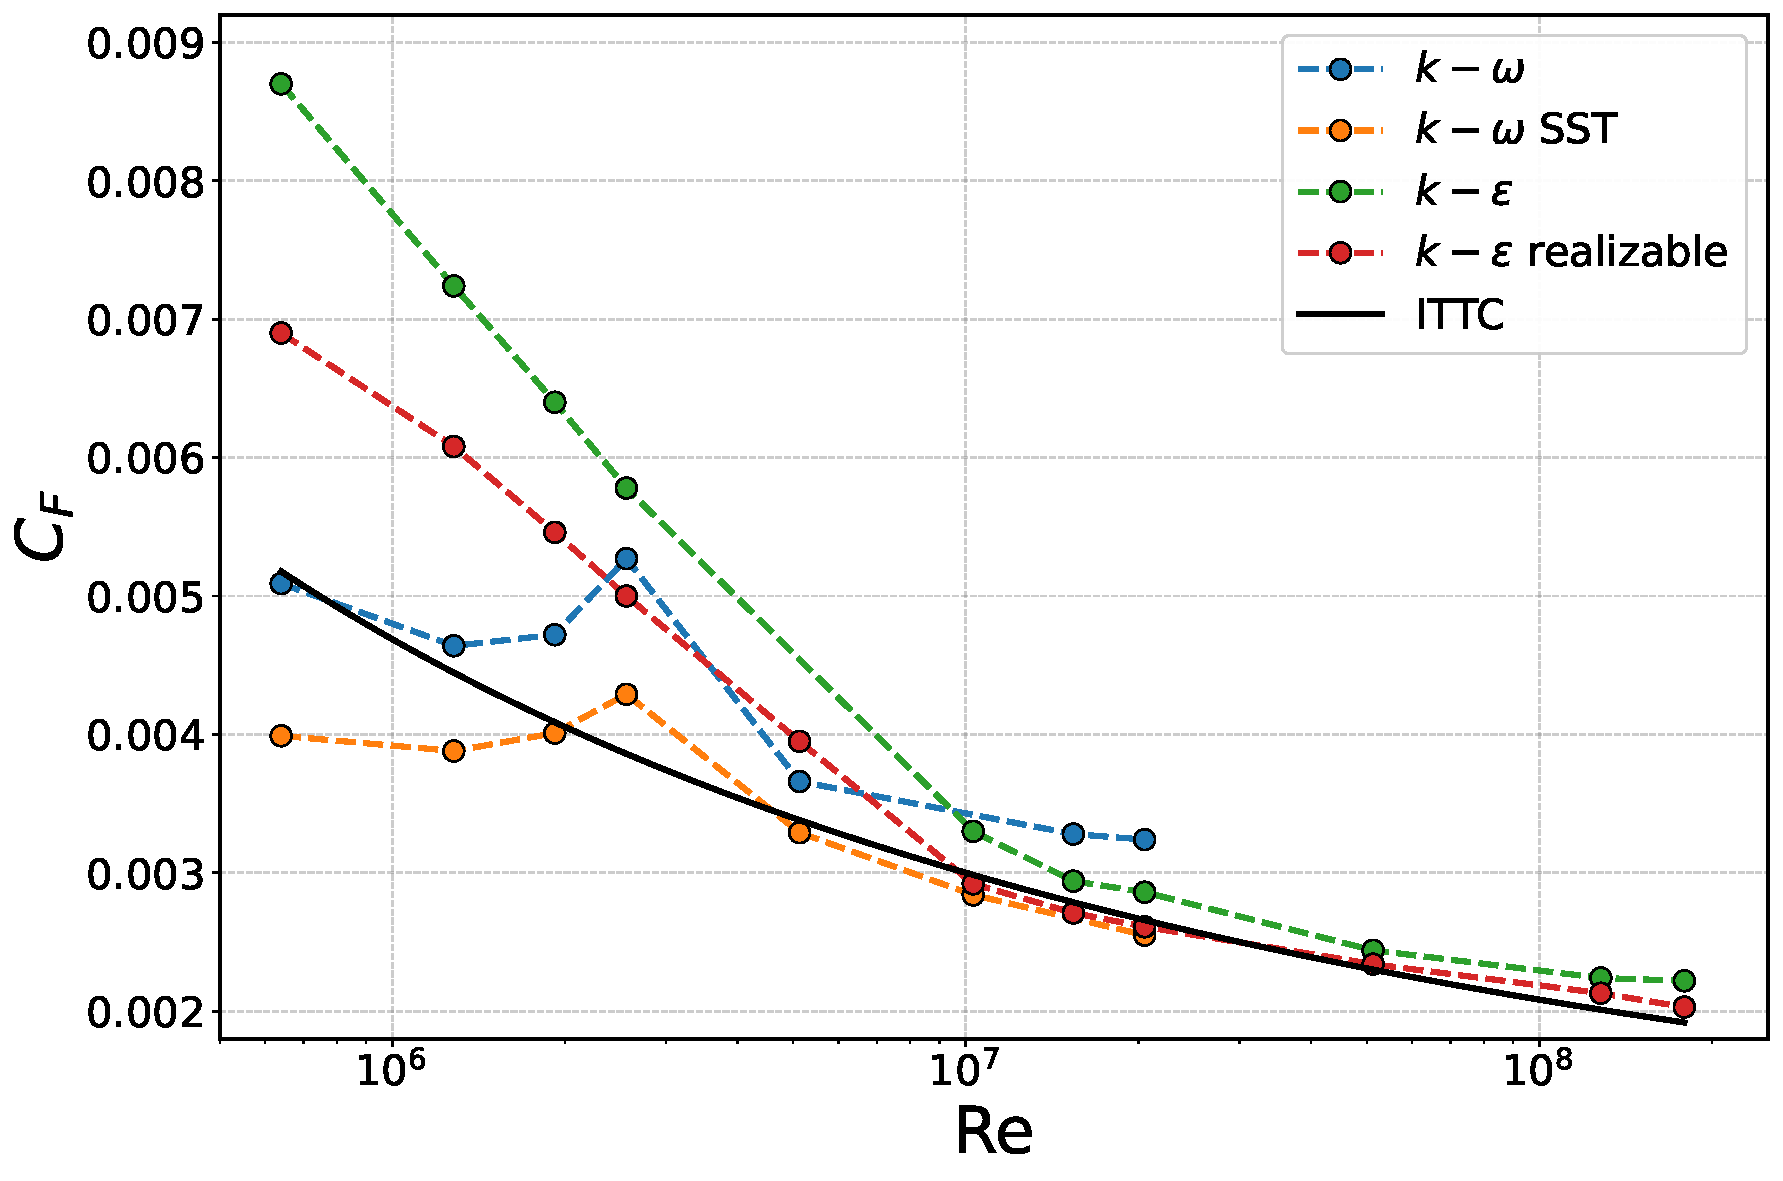
\includegraphics[width=0.75\textwidth]{images/comparacion_cf.pdf}
    \caption{Coeficiente de fricción $C_F$ en función del número de Reynolds 
    para distintos modelos de turbulencia. \textit{P1}.}
    \label{fig:comparacion_cf}
\end{figure}

\begin{figure}[htpb]
    \centering
    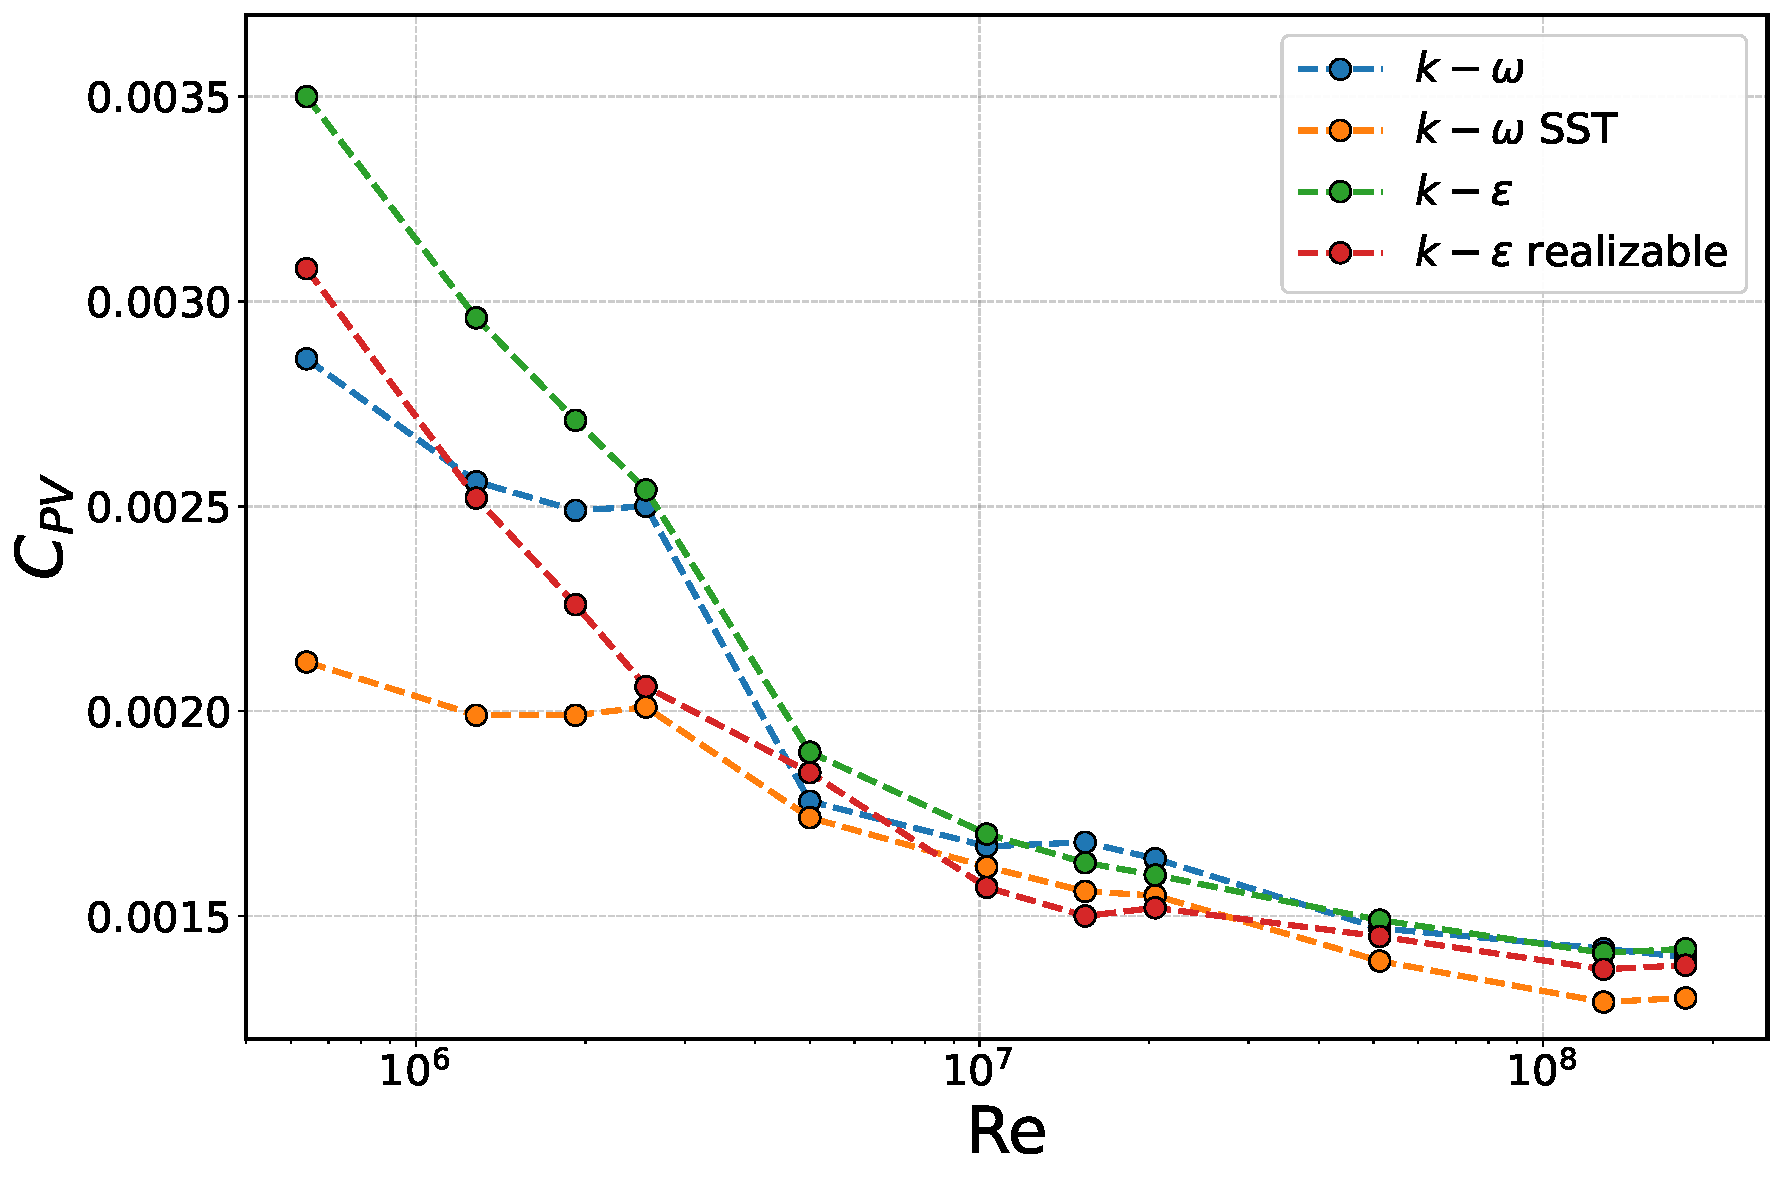
\includegraphics[width=0.75\textwidth]{images/comparacion_cp.pdf}
    \caption{Coeficiente de presión viscosa $C_{PV}$ en función del número 
    de Reynolds para distintos modelos de turbulencia. \textit{P1}.}
    \label{fig:comparacion_cp}
\end{figure}

\begin{figure}[htpb]
    \centering
    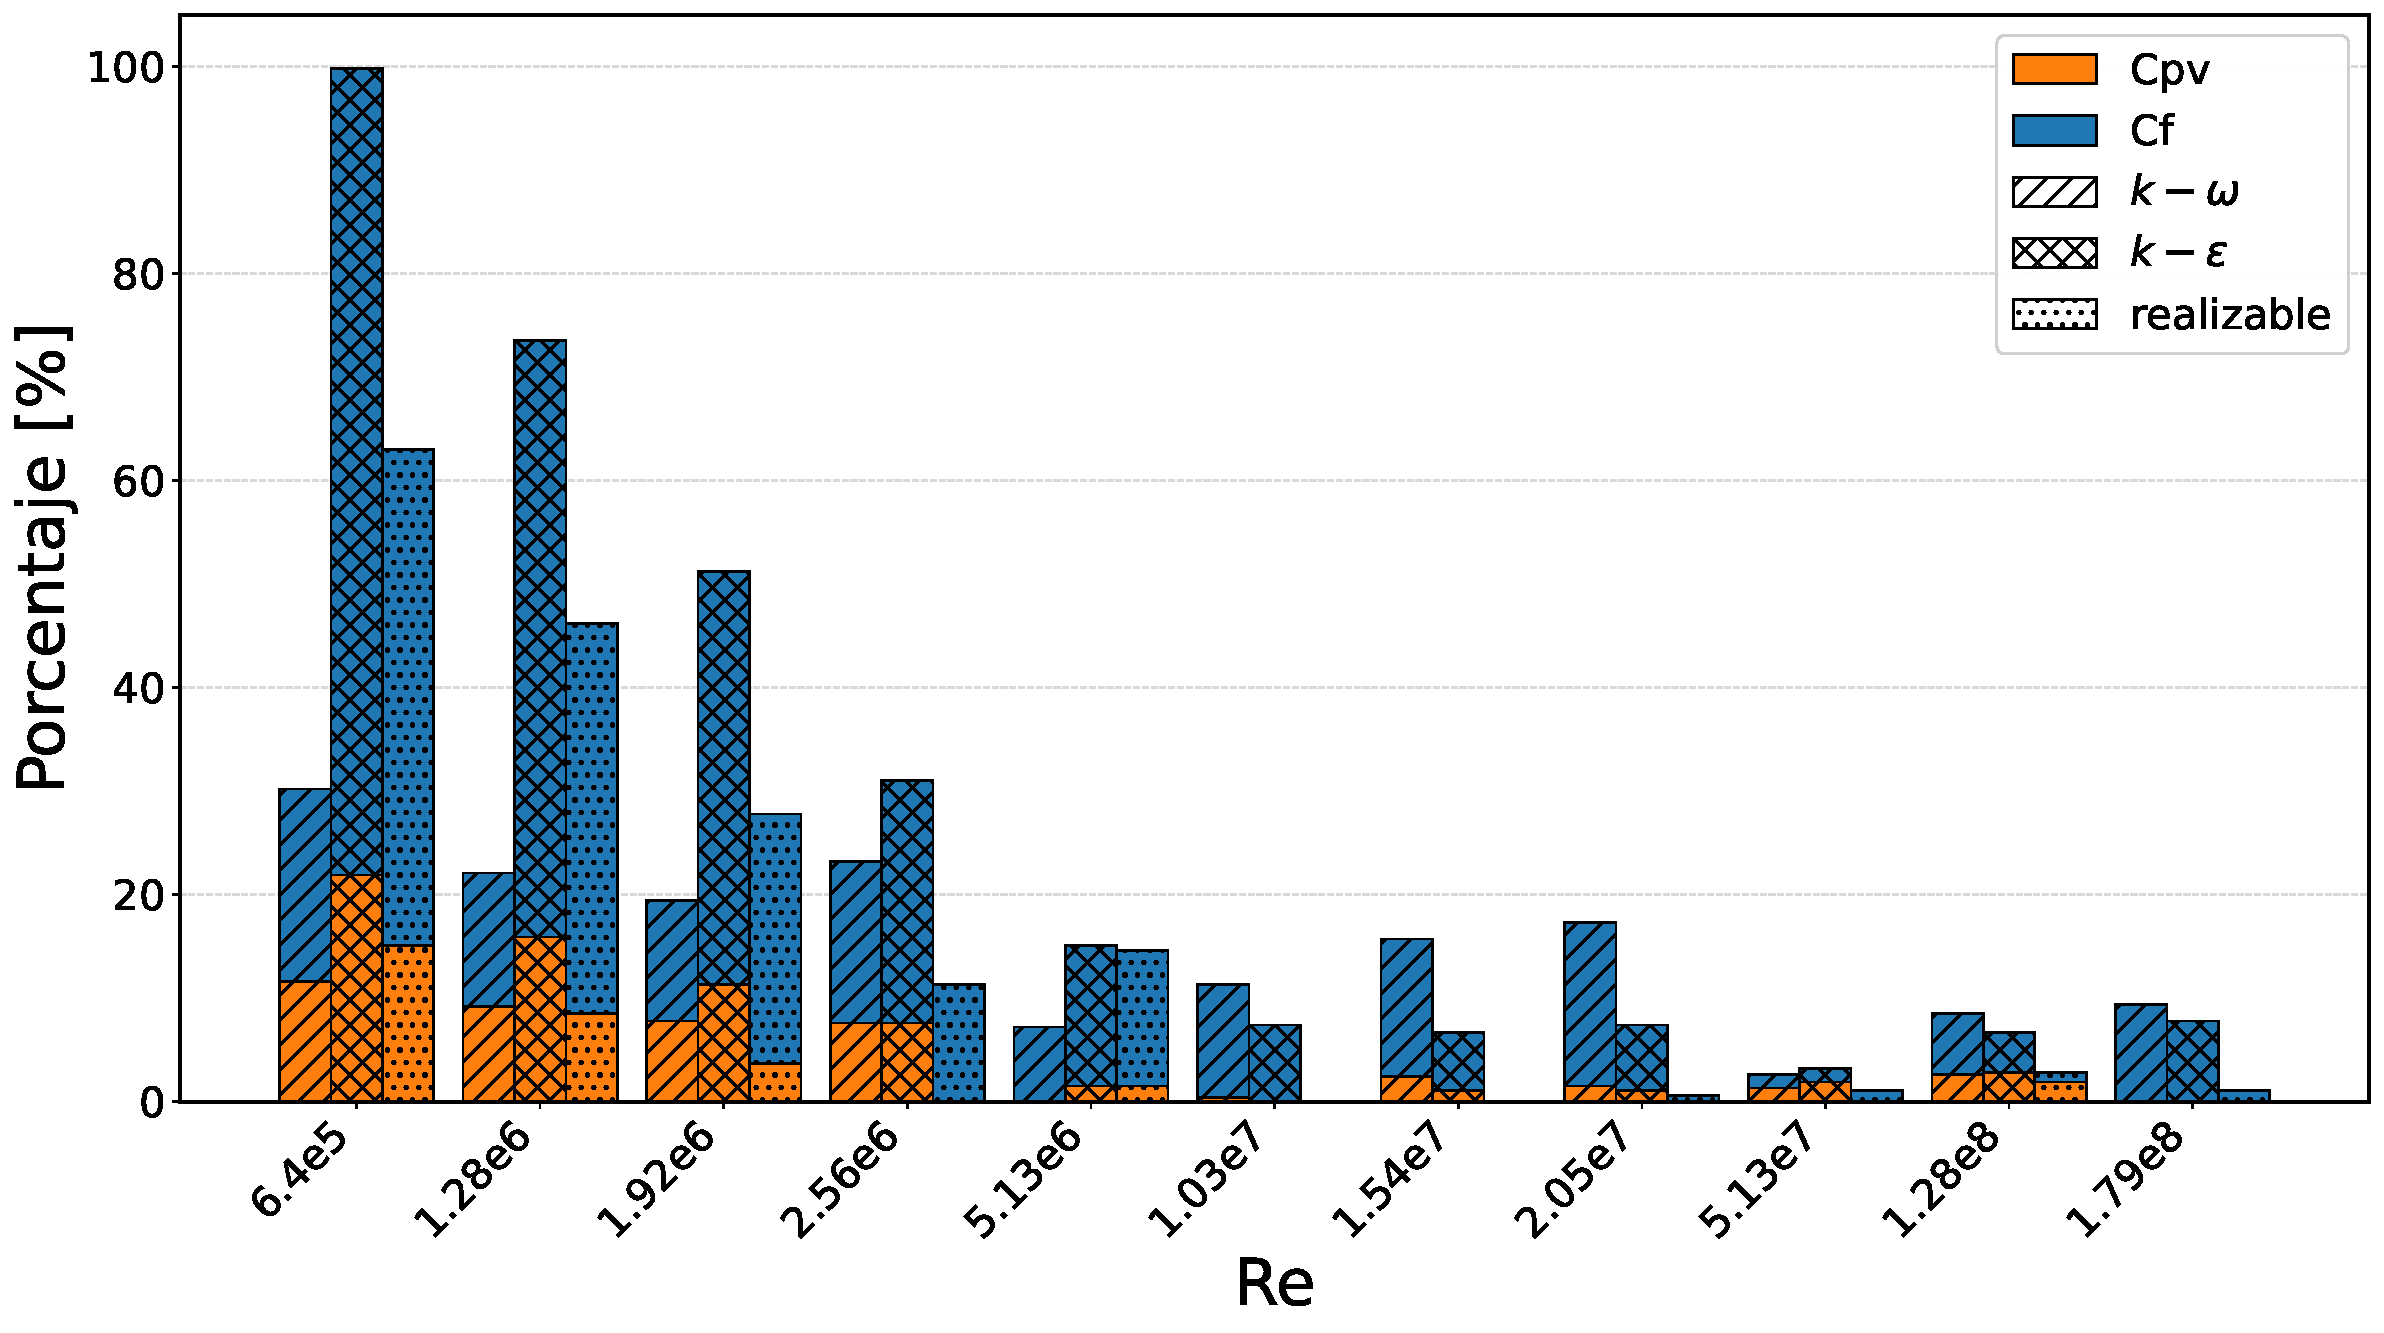
\includegraphics[width=0.85\textwidth]{images/dif_pp.pdf}
    \caption{Diferencia porcentual de $C_F$ y $C_{PV}$ respecto al modelo 
    $k$--$\omega$ SST.}
    \label{fig:dif_pp}
\end{figure}

Se observa que la mayor dispersión entre modelos ocurre a bajo $Re$, 
principalmente en la componente friccional. En ese régimen, una pequeña 
variación en $C_F$ repercute fuertemente en la estimación de $(1+k)$, dado 
que la resistencia por fricción representa la mayor parte de la resistencia 
viscosa. A medida que aumenta $Re$ y el flujo se torna plenamente turbulento, las predicciones de $C_F$ convergen a la línea ITTC-57 y la diferencia entre modelos se reduce notablemente. En cambio, $C_{PV}$ mantiene una tendencia creciente más suave con $Re$, y sus diferencias relativas entre modelos son menores pero más persistentes, lo que explica parte de la dispersión residual en el factor de forma a gran escala.

\subsection{Recomendaciones para la selección de modelos en estudios de escala}

Para estudios CFD orientados a la determinación del factor de forma mediante
extrapolación de resistencia viscosa, los resultados obtenidos permiten
formular las siguientes recomendaciones prácticas:

\begin{itemize}
    \item Priorizar modelos capaces de resolver adecuadamente la región cercana a la pared en régimen transicional, como el $k$--$\omega$ SST, 
    cuya formulación híbrida ofrece un comportamiento estable tanto en la capa límite como en el flujo externo.
    \item Mantener una resolución de malla coherente con el modelo seleccionado, especialmente en términos de $y^+$.
    \item Evaluar explícitamente la sensibilidad del factor de forma al modelo de turbulencia cuando se trabaja a bajos $Re$, en particular 
    antes de emplear $(1+k)$ como base para extrapolaciones a escala buque.
    \item Aplicar los modelos $k$--$\varepsilon$ con cautela en regímenes transicionales, dado que su mayor sensibilidad paramétrica puede 
    conducir a una sobreestimación del efecto viscoso global.
\end{itemize}

\subsection{Conclusiones parciales}

El análisis realizado permite caracterizar la influencia del modelo de turbulencia sobre la estimación de $(1+k)$ en función del régimen de flujo.
A bajos números de Reynolds, las diferencias entre modelos son significativas y afectan tanto $C_F$ como $C_{PV}$, amplificando su impacto en el valor
final del factor de forma. A medida que el flujo evoluciona hacia un régimen plenamente turbulento, esta sensibilidad se atenúa y las predicciones
convergen progresivamente.

En particular, los modelos $k$--$\varepsilon$ tienden a sobreestimar $(1+k)$ en el rango transicional, mientras que el $k$--$\omega$ SST presenta una
evolución más moderada y mejor alineada con el valor experimental. Esto confirma que la correcta interpretación del factor de forma en CFD requiere
considerar explícitamente el régimen de flujo y el modelo de turbulencia empleado, especialmente cuando los resultados se utilizan como base para
extrapolaciones o comparaciones con datos experimentales.

\section{Efecto de la relación de aspecto L/B}

\subsection{Motivación y observaciones sobre L/B en cascos de baja esbeltez}

Como se demostró en las Secciones~\ref{sec:analisis_efectos_escala} 
y~\ref{sec:descomposicion_de_la_res_viscosa}, los métodos tradicionales 
de extrapolación de resistencia, ampliamente validados para buques 
mercantes esbeltos, asumen que el factor de forma $(1+k)$ tiende a 
estabilizarse conforme aumenta el número de Reynolds. Sin embargo, este 
supuesto no se cumple para el \textit{P1}, donde las estructuras 
vorticosas longitudinales desprendidas de la quilla y el pantoque generan 
estelas más anchas y pérdidas viscosas por presión que persisten hasta la 
escala buque, impidiendo la estabilización de $(1+k)$ dentro del rango 
analizado.

En esta sección se mostrará la incapacidad de los métodos empíricos para la estimación del factor de forma en el \textit{P1} y luego se extenderá el análisis al Pesquero 2 y 3, que cuentan con distintas razones $L/B$, para identificar tendencias generalizables.

\subsection{Análisis CFD y comparación de presión y resistencia viscosa}

El comportamiento del coeficiente de presión viscosa $C_{PV}$ resulta 
determinante para comprender la evolución del factor de forma $(1+k)$ con el 
número de Reynolds. Esto se observó claramente al comparar el \textit{P1} con 
el KCS, como fue presentado en la Figura~\ref{cpv_friccion}. Si bien $C_{PV}$ 
disminuye con $Re$ de manera similar en ambos cascos en términos absolutos, 
la proporción que $C_{PV}$ representa dentro de $C_V$ es sustancialmente 
mayor en el \textit{P1} que en el KCS a lo largo de todo el rango de escalas 
analizado.

Esta diferencia responde a la dificultad del flujo para recuperar la presión 
en la popa del \textit{P1}, donde se generan grandes estructuras vorticosas 
que persisten aun a escala buque. En el KCS, $C_F$ domina ampliamente sobre 
$C_{PV}$, de modo que $(1+k) = C_V/C_{F0}$ queda gobernado por el 
comportamiento de $C_F$, que sigue de cerca a $C_{F0}$ y produce un cociente 
prácticamente constante. En el \textit{P1}, en cambio, $C_F$ y $C_{PV}$ son 
de magnitud comparable, y la caída más lenta de $C_{PV}$ respecto a $C_{F0}$ 
impide que el cociente se estabilice dentro del rango de escalas analizado.

Al comparar el valor de $(1+k)$ obtenido para el \textit{P1} con 
correlaciones empíricas desarrolladas para buques mercantes, surge una 
doble inconsistencia. Por un lado, el valor de $(1+k) \approx 1{.}73$ 
obtenido por CFD DB a escala buque no tiene precedente en la literatura 
de hidrodinámica naval: no se ha encontrado un valor comparable para 
ningún casco desnudo documentado hasta la fecha. Por otro lado, las 
fórmulas empíricas consideradas fueron desarrolladas a partir de ensayos 
con buques mercantes de esbeltez convencional. Entre los parámetros 
geométricos de entrada de estas correlaciones ($C_B$, $L/B$, $B/T$, 
$S/L^2$, $L/\nabla^{1/3}$), la relación $L/B = 3{.}75$ del \textit{P1} 
resulta notablemente inferior a la de los buques mercantes típicos para 
los cuales fueron calibradas, lo que compromete la aplicabilidad de estas 
expresiones a este tipo de casco. Como consecuencia, las fórmulas 
disponibles no reproducen los altos valores observados mediante CFD DB 
para escala buque. La Tabla~\ref{tab:empiricos} presenta las expresiones 
utilizadas y los valores obtenidos para el \textit{P1}, y la 
Figura~\ref{empiricos} ilustra la alta dispersión entre correlaciones y 
la falta de coincidencia con los resultados numéricos y experimentales.

\begin{table}[htpb]
\centering
\caption{Correlaciones empíricas para la estimación del factor de forma 
$(1+k)$ y valores obtenidos para el \textit{P1} 
($L = 34{.}8$~m, $B = 9{.}28$~m, $T = 3{.}9$~m, 
$S = 449{.}6$~m$^2$, $C_B = 0{.}64$, $\nabla = 152{.}0$~m$^3$).}
\label{tab:empiricos}
\small
\begin{tabularx}{\textwidth}{lXc}
\toprule
\textbf{Método} & \textbf{Expresión} & \boldmath{$(1+k)$} \\
\midrule
\citet{molland2017ship} (Watanabe) &
$\displaystyle 1 + k = 1 - 0{.}095 + 
\frac{25{.}6\,C_B}{(L/B)^2\,\sqrt{B/T}}$ &
$1{.}660$ \\[10pt]

\citet{conn1968results} &
$\displaystyle 1 + k = 1 + 18{.}7
\left(\frac{C_B\,B}{L}\right)^{2}$ &
$1{.}545$ \\[10pt]

\citet{grigson2000planar} &
$\displaystyle 1 + k = 1 + 0{.}028 + 3{.}3\,
\frac{S}{L^2}\sqrt{\frac{C_B\,B}{L}}$ &
$1{.}534$ \\[10pt]

\citet{wright1984viscous} &
$\displaystyle 1 + k = 2{.}48\,
C_B^{0{.}1526}\,
\left(\frac{B}{T}\right)^{0{.}0533}\,
\left(\frac{B}{L}\right)^{0{.}3856}$ &
$1{.}457$ \\[10pt]

\citet{couser1997calm} &
$\displaystyle 1 + k = 2{.}76\,
\left(\frac{L}{\nabla^{1/3}}\right)^{-0{.}4}$ &
$1{.}616$ \\[10pt]

Prohaska (EFD, presente trabajo) & --- & $1{.}19$ \\
\bottomrule
\end{tabularx}
\end{table}

\begin{figure}[htpb]
    \centering
    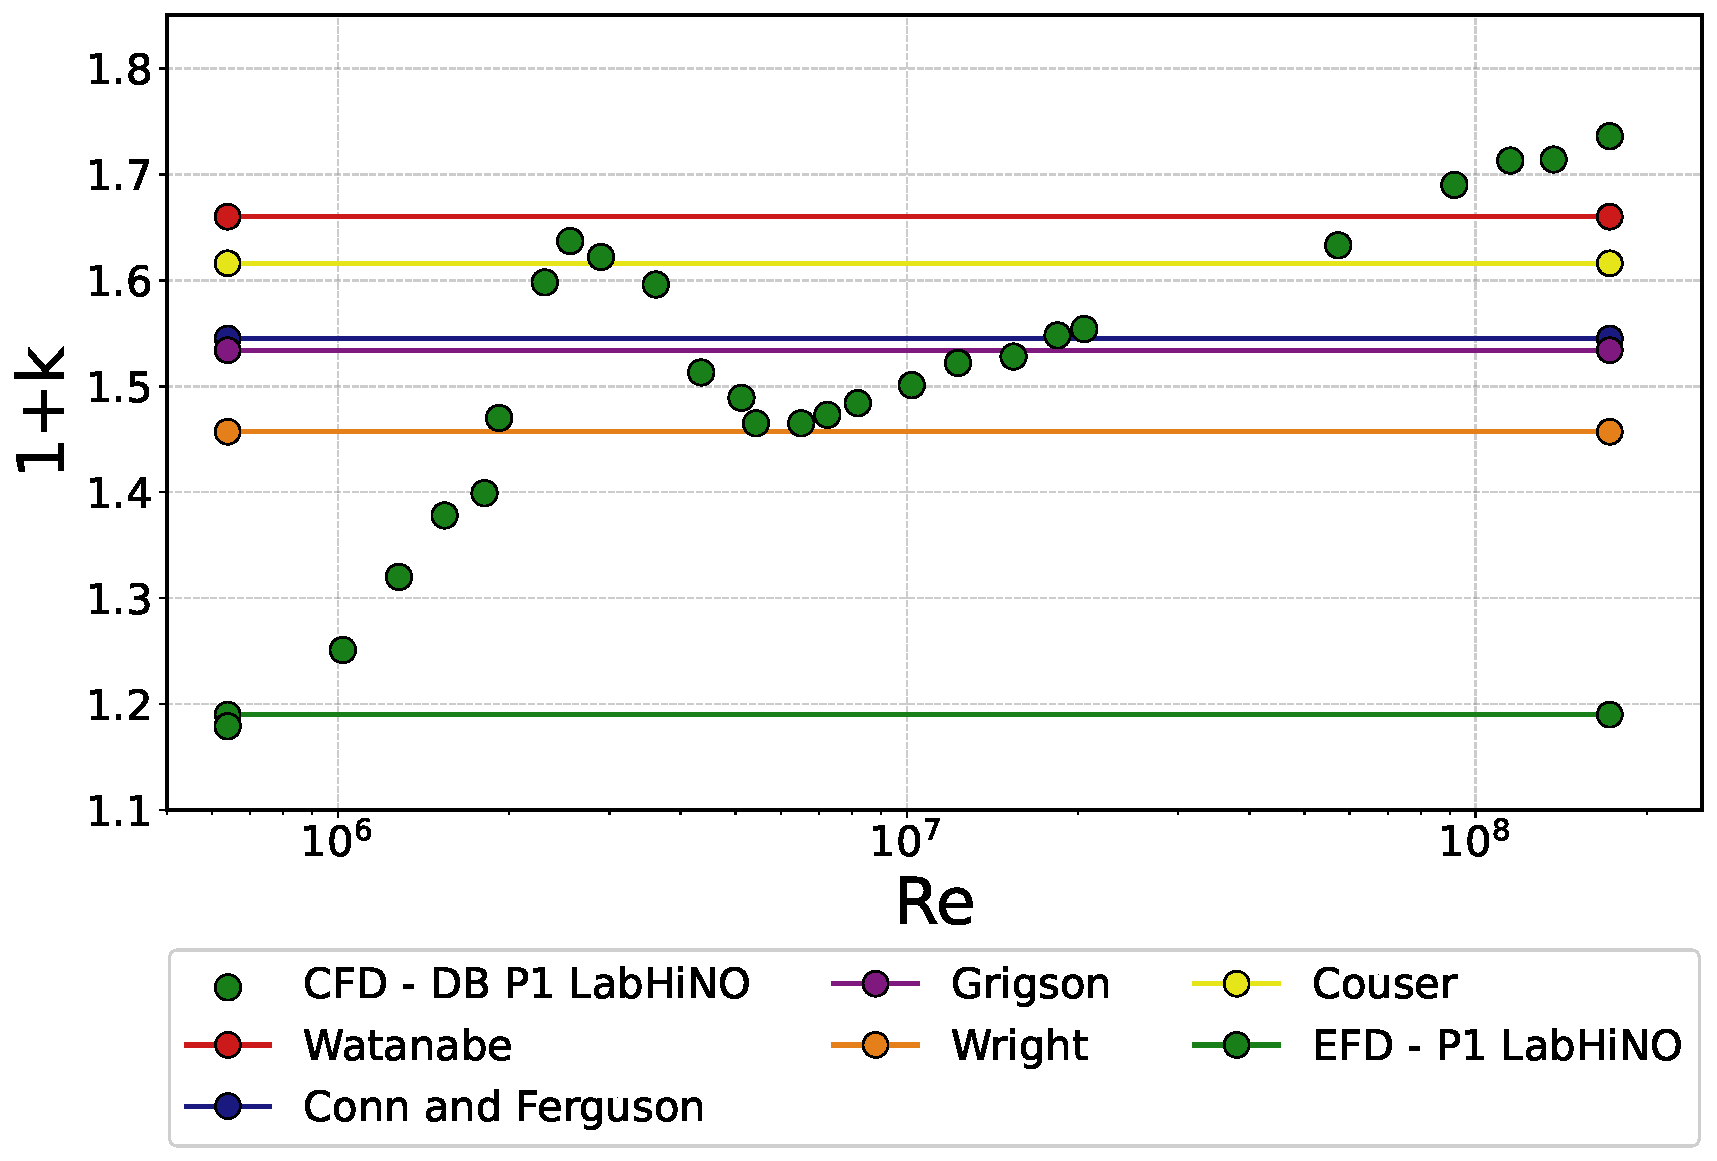
\includegraphics[width=.6\textwidth]{./images/empiricos.pdf}
    \caption{Valores de $(1+k)$ para el \textit{P1} en función de $Re$, 
    obtenidos por CFD DB, EFD y correlaciones empíricas de la literatura 
    \citep{molland2017ship, conn1968results, grigson2000planar, 
    wright1984viscous, couser1997calm}.}
    \label{empiricos}
\end{figure}

Estas dos observaciones en conjunto, la ausencia de valores comparables 
en la literatura naval y la inaplicabilidad de las correlaciones 
existentes, motivaron la búsqueda de referencias en otros ámbitos donde 
la geometría controla la resistencia viscosa y donde se manejan cuerpos 
de baja esbeltez. En aerodinámica, el método clásico de estimación de 
resistencia de fuselajes consiste en multiplicar el coeficiente de 
fricción turbulenta de placa plana por un factor de forma empírico 
dependiente de la razón de esbeltez del cuerpo, y por el área mojada. 
El fuselaje se modela como un cuerpo de revolución, y el parámetro 
geométrico principal es la razón de esbeltez $l/d$, directamente análoga 
a $L/B$ en cascos de buques. \citet{hoerner1965drag} fue el primero en 
derivar un factor de forma para cuerpos de revolución a partir de 
correlaciones con ensayos en túnel de viento, obteniendo una curva válida 
para $l/d > 4.5$ que fue extrapolada hacia valores menores sin validación 
experimental. Autores posteriores \citep{raymer2019aircraft, 
torenbeek2010synthesis, roskam1987airplane, shevell1989fundamentals} 
continuaron ajustando estas correlaciones para extender su rango de 
validez hacia cuerpos menos esbeltos. La Figura~\ref{aerodynamics} 
superpone estas correlaciones con los valores de $(1+k)$ a escala buque 
obtenidos por CFD DB para el \textit{P1} ($L/B = 3.53$) y para el KCS 
($L/B = 7.14$, datos de \citet{TerzievDataSet}), representados en 
función de $l/d = L/B$.

La Tabla~\ref{tab:aerodinamicos} presenta las expresiones de las 
correlaciones aerodinámicas consideradas en la Figura~\ref{aerodynamics}.

\begin{table}[htpb]
\centering
\caption{Correlaciones aerodinámicas de factor de forma para cuerpos de 
revolución en función de la razón de esbeltez $l/d$.}
\label{tab:aerodinamicos}
\small
\begin{tabularx}{\textwidth}{lX}
\toprule
\textbf{Método} & \textbf{Expresión} \\
\midrule
\citet{hoerner1965drag} &
$\displaystyle \mathrm{FF} = 1 + 
\frac{1{.}5}{(l/d)^{1{.}5}} + 
\frac{7}{(l/d)^{3}}$ \\[10pt]

\citet{torenbeek2010synthesis} &
$\displaystyle \mathrm{FF} = 1 + 
\frac{2{.}2}{(l/d)^{1{.}5}} + 
\frac{3{.}8}{(l/d)^{3}}$ \\[10pt]

\citet{shevell1989fundamentals} &
$\displaystyle \mathrm{FF} = 2{.}939 - 0{.}7666\,\frac{l}{d} + 
0{.}1328\left(\frac{l}{d}\right)^{2}
- 0{.}01074\left(\frac{l}{d}\right)^{3}
+ 3{.}275\times10^{-4}\left(\frac{l}{d}\right)^{4}$ \\[10pt]

\citet{raymer2019aircraft} (Raymer new) &
$\displaystyle \mathrm{FF} = 0{.}9 + 0{.}0025\,\frac{l}{d} + 
\frac{5}{(l/d)^{1{.}5}}$ \\[10pt]

\citet{roskam1987airplane} &
$\displaystyle \mathrm{FF} = 1 + 0{.}0025\,\frac{l}{d} + 
\frac{60}{(l/d)^{3}}$ \\
\bottomrule
\end{tabularx}
\end{table}

\begin{figure}[htpb]
    \centering
    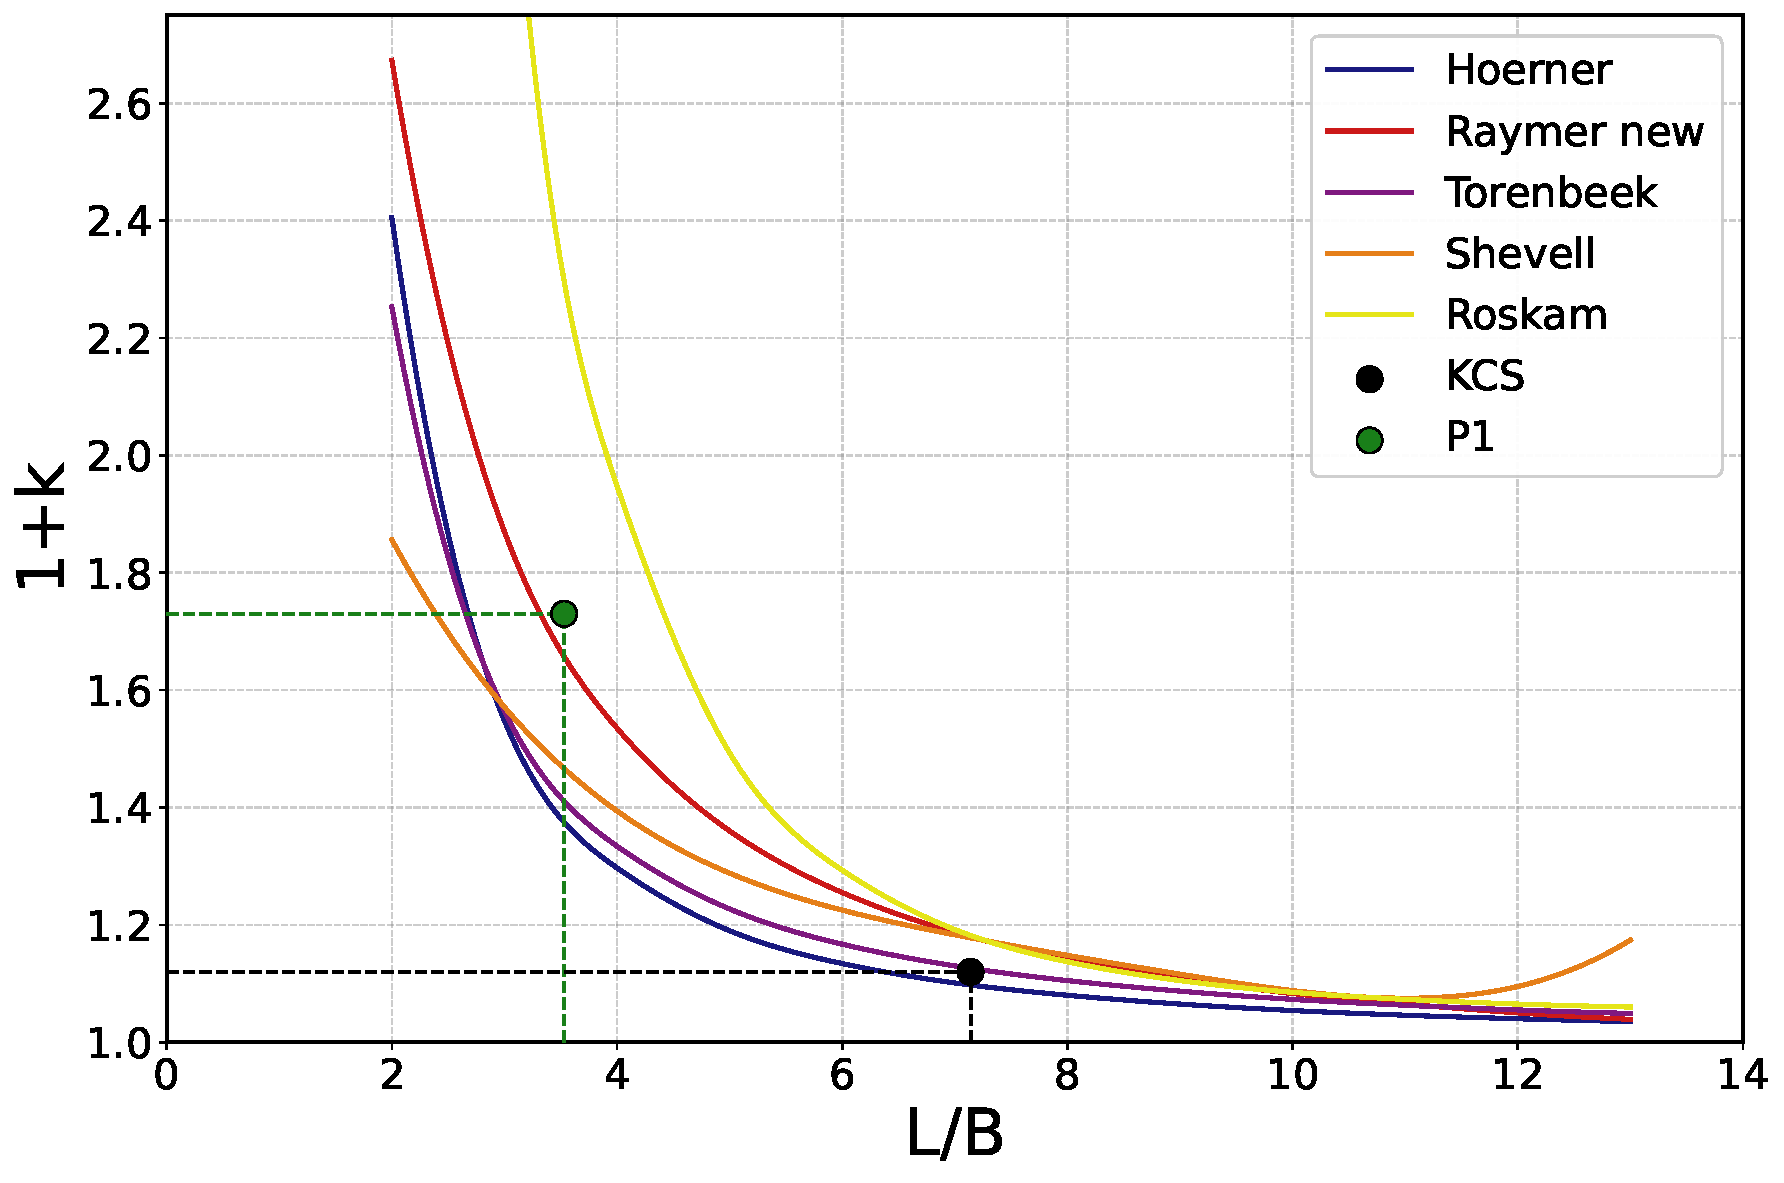
\includegraphics[width=.6\textwidth]{./images/aerodynamics.pdf}
    \caption{Factores de forma para cuerpos de revolución en función de la 
    razón de esbeltez $l/d$ y comparación con valores CFD DB para el 
    \textit{P1} y el KCS. Datos de \citep{hoerner1965drag, 
    raymer2019aircraft, torenbeek2010synthesis, roskam1987airplane, 
    shevell1989fundamentals, TerzievDataSet}.}
    \label{aerodynamics}
\end{figure}

El valor del KCS coincide con la curva de \citet{hoerner1965drag}, coherente 
con su alta esbeltez y con el rango para el que dicha curva fue derivada 
originalmente. El valor del \textit{P1}, en cambio, muestra mayor afinidad 
con la curva ``Raymer New'' \citep{raymer2019aircraft}, ajustada 
específicamente para cuerpos de menor esbeltez. Es notable que correlaciones 
provenientes de un campo de estudio diferente, pero que incluyen valores de 
$l/d$ suficientemente bajos como para abarcar la geometría del \textit{P1}, 
reproduzcan los resultados CFD con mayor fidelidad que las correlaciones 
navales tradicionales.

Este hallazgo sugiere que, para cascos con baja razón $L/B$, las 
correlaciones aerodinámicas representan mejor la dependencia geométrica del 
factor de forma que las correlaciones navales tradicionales, desarrolladas 
para valores de $L/B$ significativamente más altos.


\subsection{Presentación de pesqueros con distintos L/B}

Los tres pesqueros analizados en esta tesis, presentados en la 
Sección~\ref{sec:presentacion_modelos} junto con el KCS, fueron 
seleccionados precisamente por cubrir un rango de relaciones de esbeltez 
$L/B$ distintas: $3{.}53$ (\textit{P1}), $3{.}23$ (\textit{P2}) y 
$2{.}85$ (\textit{P3}). Esta diversidad geométrica permite evaluar de 
manera sistemática si el comportamiento observado para el \textit{P1} 
constituye un caso aislado o refleja una tendencia estructural asociada 
a la baja esbeltez. La Figura~\ref{fig:LB_comparisson} presenta las 
cuatro geometrías escaladas a la misma eslora, con el fin de resaltar 
las diferencias morfológicas asociadas al ancho relativo, volumen 
transversal y forma de popa.

\begin{figure}[h!]
    \centering
    % --- Primera columna: nombres ---
    \begin{subfigure}{.18\textwidth}
        \centering
        \vspace{1em}
        \footnotesize % controla el tamaño de texto
        \textbf{KCS (L/B = 7.12)}\\[3em]
        \textbf{Fishing Vessel 1 (L/B = 3.53)}\\[3.5em]
        \textbf{Fishing Vessel 2 (L/B = 3.23)}\\[3.5em]
        \textbf{Fishing Vessel 3 (L/B = 2.85)}
        \caption*{ }
    \end{subfigure}
    % --- Segunda columna: vista frontal ---
    \begin{subfigure}{.15\textwidth}
        \centering
        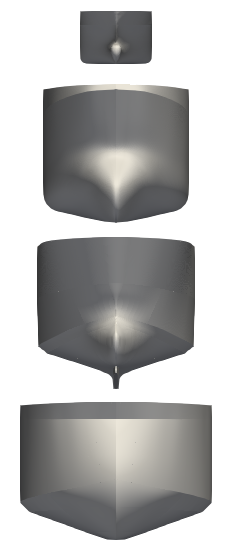
\includegraphics[width=\linewidth]{./images/L-B-front.png}
        \caption{Front view}
    \end{subfigure}%
    % --- Tercera columna: vista lateral ---
    \begin{subfigure}{.395\textwidth}
        \centering
        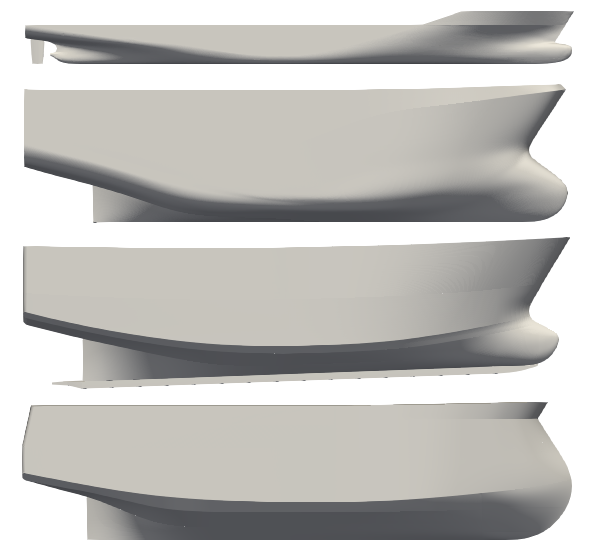
\includegraphics[width=\linewidth]{./images/L-B-side.png}
        \caption{Side view}
    \end{subfigure}
    \begin{subfigure}{.24\textwidth}
        \centering
        \vspace{1em}
        \footnotesize % controla el tamaño de texto
        \textbf{L = 230m , B = 32.2m \\ $\lambda$ = 1:79}\\[3em]
        \textbf{L = 34.79m , B = 9.28m \\ $\lambda$ = 1:20 }\\[3.5em]
        \textbf{L = 27.6m , B = 7.8m \\ $\lambda$ = 1:10}\\[3.5em]
        \textbf{L= 22.3m , B = 7.8m \\ $\lambda$ = 1:13}
        \caption*{ }
    \end{subfigure}
    \caption{Tested models. The four hulls are shown scaled to equal length for direct comparison.}
    \label{fig:LB_comparisson}
\end{figure}

Al disminuir $L/B$, las secciones transversales se vuelven más robustas y la transición hacia la popa más abrupta, lo que favorece la aparición de regiones extensas de presión adversa y el desprendimiento de estructuras vorticosas de gran escala. Estas características inducen mayores valores de $C_{PV}$ y explican la persistencia de la presión viscosa incluso a escala buque. A pesar de sus diferencias individuales, los tres pesqueros comparten proporciones y distribución volumétrica similares, lo que sugiere la presencia de un comportamiento hidrodinámico común asociado a la baja esbeltez.


\subsection{Generalización del comportamiento observado y formulación empírica}\label{sec:generalizacion_LB}

Como se mostró en la Figura~\ref{fig:Re_formfactor} de la 
Sección~\ref{sec:analisis_efectos_escala}, los tres pesqueros presentan 
un crecimiento continuo y no asintótico de $(1+k)$ incluso hacia escala 
buque, en marcado contraste con el KCS, que exhibe el incremento inicial 
y posterior estabilización esperados conforme se desarrolla la capa límite 
turbulenta.

La consistencia entre los tres modelos confirma que este comportamiento no es propio de un caso aislado, sino un rasgo estructural de cascos con $L/B < 4$. A medida que disminuye la esbeltez, aumenta el componente de presión viscosa y, en consecuencia, el factor de forma. La tendencia creciente y no asintótica en los pesqueros sugiere que la influencia de la presión viscosa domina su comportamiento hidrodinámico incluso en condiciones de escala buque.

Para interpretar esta dependencia geométrica, se recurrió nuevamente a correlaciones aerodinámicas desarrolladas para cuerpos de revolución, donde el factor de forma se expresa en función de la razón de esbeltez $l/d$. La Figura~\ref{fig:aero_comparison_full} incorpora simultáneamente las diferentes curvas aerodinámicas clásicas junto con los valores de $(1+k)$ provenientes de CFD DB para los cuatro cascos estudiados, todos representados en términos de $l/d = L/B$.

\begin{figure}[h]
    \centering
    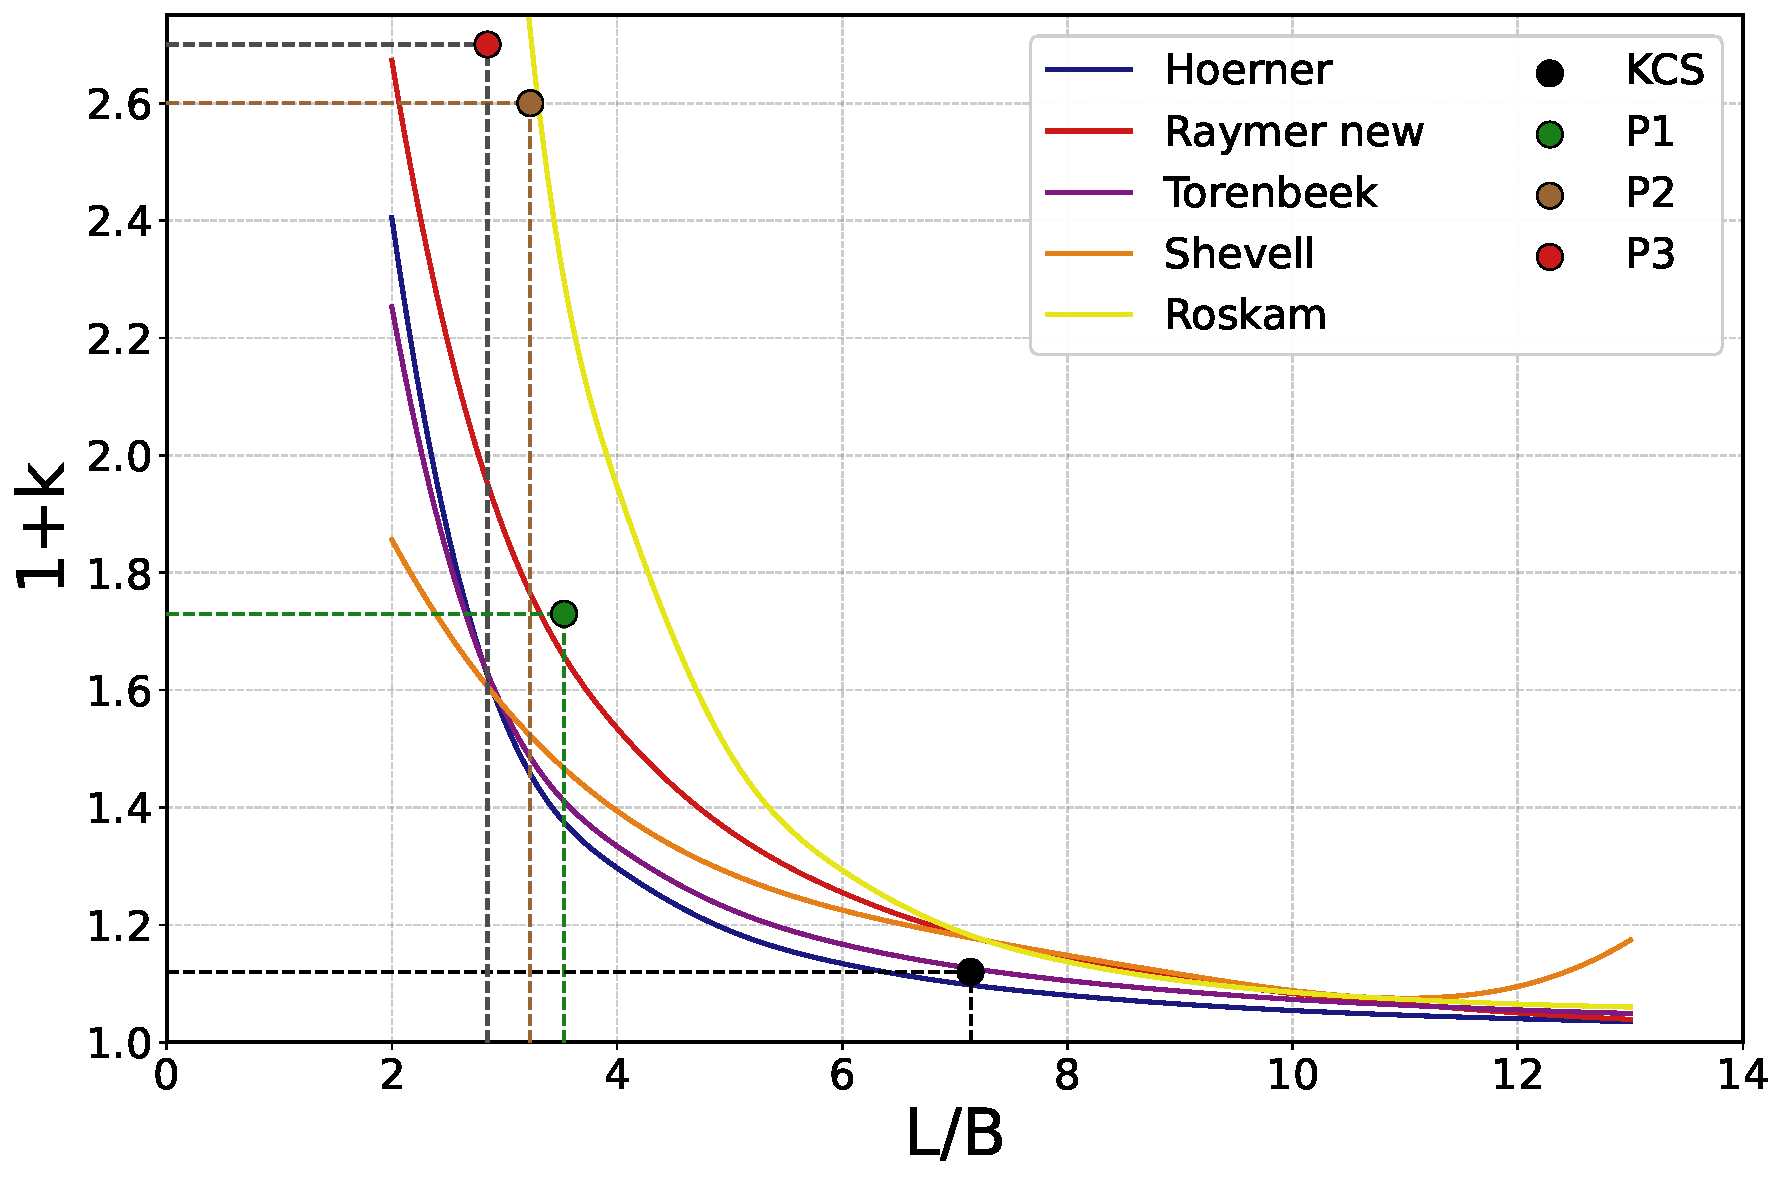
\includegraphics[width=.6\textwidth]{./images/aerodynamics2.pdf}
    \caption{Comparación entre correlaciones aerodinámicas de factor de forma y los valores $(1+k)$ obtenidos mediante CFD DB para los tres pesqueros y el KCS, representados en función de $l/d = L/B$.}
    \label{fig:aero_comparison_full}
\end{figure}

El gráfico revela una tendencia clara:  
\begin{itemize}
    \item El valor correspondiente al KCS se ubica en la región de altas esbelteces y coincide con la curva clásica de Hoerner, como era de esperar para un casco alargado.
    \item Los tres pesqueros, caracterizados por $L/B < 4$, se agrupan en la región de cuerpos poco esbeltos y exhiben proximidad a las correlaciones propuestas por \cite{roskam1987airplane} y \cite{raymer2019aircraft}.
    \item La alineación de los tres pesqueros refuerza la existencia de un mecanismo geométrico común que explica sus elevados valores de $(1+k)$.
\end{itemize}

Estos resultados sugieren que, para cascos de baja esbeltez, la relación entre $(1+k)$ y $L/B$ se comporta de manera análoga a la que se observa en cuerpos de revolución evaluados en aerodinámica. En consecuencia, la utilización directa de correlaciones aerodinámicas provee un marco más apropiado para interpretar la evolución del factor de forma en esta clase de buques que las fórmulas navales tradicionales, desarrolladas para valores significativamente más altos de $L/B$.

Este hallazgo abre la posibilidad de desarrollar una formulación empírica específica para pesqueros de baja esbeltez que permita predecir el comportamiento de $(1+k)$ a escala buque sin necesidad de extrapolar correlaciones que fueron diseñadas en base a buques considerablemente más esbeltos.


\subsection{Implicancias para el escalado y la extrapolación de resultados}

La marcada dependencia del factor de forma con el número de Reynolds, 
observada en los pesqueros analizados, tiene consecuencias directas sobre 
la extrapolación de resistencia y la estimación de la potencia efectiva a 
escala buque. En particular, los valores elevados de $(1+k)$ obtenidos para 
estos cascos, junto con su crecimiento sostenido hacia altas escalas, 
desafían el supuesto central del método ITTC: la igualdad entre los factores 
de forma del modelo y del buque ($k_{M} = k_{S}$).

Como se desarrolla en la Sección~\ref{sec:prediccion_potencia}, el 
procedimiento estándar de predicción de potencia \citep{ITTC_Performance_prediction} 
estima la resistencia total del buque como:
%
\begin{equation}
    C_{TS} = (1 + k_S)\,C_{FS0} + C_W + \Delta C_F + C_A
\end{equation}
%
donde $C_{FS0}$ es el coeficiente de fricción del buque calculado mediante 
la línea ITTC-57, $C_W$ es el coeficiente de resistencia por formación de 
olas obtenido del modelo físico como residuo de la descomposición viscosa, 
y $\Delta C_F$ y $C_A$ corresponden a las correcciones por rugosidad y 
correlación recomendadas por la ITTC. Este método supone que $k_S = k_M$, 
es decir, que el factor de forma es independiente de la escala.

Sin embargo, los resultados CFD DB demostraron que este supuesto no se 
cumple para los pesqueros estudiados. El fuerte incremento de $(1+k)$ con 
$Re$ implica que:
%
\begin{equation}
    k_S \gg k_M,
\end{equation}
%
lo que significa que la extrapolación tradicional subestima sistemáticamente 
la resistencia viscosa del buque y, por ende, la potencia efectiva necesaria.

La resistencia total del buque a escala buque y la potencia efectiva se 
obtienen como (Sección~\ref{sec:prediccion_potencia}):
%
\begin{equation}
    R_{TS} = \tfrac{1}{2}\,\rho\,V_S^2\,S_S\,C_{TS}
\end{equation}
%
\begin{equation}
    P_{ES} = R_{TS}\,V_S
\end{equation}
%
donde $\rho$ es la densidad del agua, $V_S$ la velocidad del buque y $S_S$ 
la superficie mojada a escala buque.

Para cuantificar la magnitud del error introducido por la selección de un valor inapropiado de $k$, se compararon tres enfoques (Tablas~\ref{tbl:metodos_abs} y \ref{tbl:metodos_delta}):

\begin{itemize}
    \item \textbf{Método 1 (ITTC–EFD)}: $k_M = k_S$, obtenido por el método de Prohaska en modelo.
    \item \textbf{Método 2 (CFD–EFD, doble k)}: valores distintos de $k_M$ y $k_S$, determinados mediante CFD DB para modelo y buque. La idea es propuesta por \cite{korkmaz_wetted_transom} pero en su caso la diferencia nace exclusivamente de la popa sumergida, mientras que según la presente tesis la necesidad surge de los efectos de escala presentados en la Sección \ref{sec:descomposicion_de_la_res_viscosa} (Cpv).
    \item \textbf{Método 3 ($k = 0$)}: empleado cuando no es posible determinar el factor de forma ni experimentalmente ni mediante CFD; asume resistencia viscosa puramente friccional, equivalente a tratar el casco como una placa plana. Provee una cota de referencia para cuantificar el error asociado a ignorar completamente los efectos de forma.

\end{itemize}

\begin{table*}[htbp]
\caption{$C_{TS}$, $R_{TS}$ y $P_{ES}$ estimados mediante tres enfoques distintos para velocidades de operación del \textit{P1}.}

\label{tbl:metodos_abs}
\scriptsize
\centering

\begin{tabular}{c c c
    r r r
    r r r
    r r r}
\toprule
\multirow{2}{*}{$Fr$} &
\multicolumn{2}{c}{Velocidad} &
\multicolumn{3}{c}{Method 1 (EFD)} &
\multicolumn{3}{c}{Method 2 (EFD--CFD)} &
\multicolumn{3}{c}{Method 3 ($k=0$)} \\
\cmidrule(lr){2-3}
\cmidrule(lr){4-6}
\cmidrule(lr){7-9}
\cmidrule(lr){10-12}
 & $v_S$ & $v_S$ &
 $C_{TS}$ & $R_{TS}$ & $P_{ES}$ &
 $C_{TS}$ & $R_{TS}$ & $P_{ES}$ &
 $C_{TS}$ & $R_{TS}$ & $P_{ES}$ \\
 & {[m/s]} & {[kn]} &
 & {[kN]} & {[kW]} &
 & {[kN]} & {[kW]} &
 & {[kN]} & {[kW]} \\
\midrule
0.26 & 4.71 & 9.16
     & 6.28 & 32.16 & 151.51
     & 7.33 & 37.53 & 176.79
     & 6.70 & 34.27 & 161.46 \\
0.30 & 5.34 & 10.38
     & 7.68 & 50.46 & 269.34
     & 8.71 & 57.22 & 305.45
     & 8.08 & 53.08 & 283.34 \\
\bottomrule
\end{tabular}
\end{table*}

\begin{table}[htbp]
\caption{Diferencias porcentuales en la potencia efectiva estimada respecto al método ITTC (Método 1).}
\label{tbl:metodos_delta}
\scriptsize
\centering

\begin{tabular}{c c c c c}
\toprule
$Fr$ & $v_S$ & $v_S$ & Method 2 vs 1 & Method 3 vs 1 \\
     & {[m/s]} & {[kn]} & {$\Delta P_{ES}$ [\%]} & {$\Delta P_{ES}$ [\%]} \\
\midrule
0.26 & 4.71 & 9.16  & 16.7 & 6.6 \\
0.30 & 5.34 & 10.38 & 13.4 & 5.2 \\
\bottomrule
\end{tabular}

\end{table}




Los resultados muestran que asumir $k=0$ (método 3) produce una sobreestimación de la potencia efectiva de aproximadamente $5\%$ respecto al método estándar ITTC. Como era de esperar, este método sobreestima la resistencia al ignorar la contribución viscosa de la forma del casco; sin embargo, su utilidad radica en que provee una referencia cuando no se dispone de ningún ensayo ni simulación para estimar el factor de forma, permitiendo acotar el error esperado.

En cambio, el método de doble $k$ basado en CFD DB (método 2) arroja una \textbf{potencia un 13–17$\%$ mayor} que la obtenida mediante el enfoque ITTC (método 1), diferencia atribuible al mayor valor de $k_S$ predicho numéricamente.

Estas discrepancias, del orden del 15$\%$ en términos de potencia instalada, son suficientemente significativas como para justificar una validación mediante pruebas de mar. Además, sugieren que las correlaciones empíricas introducidas en la Sección \ref{sec:generalizacion_LB}, originadas en aeronáutica y dependientes de la razón de esbeltez, podrían ser utilizadas como una estimación preliminar de $k_S$ de forma más confiable que las metodologías navales actuales. Esto permitiría implementar un método de extrapolación de doble $k$, donde $k_M$ se obtenga de CFD DB a escala modelo y $k_S$ de una correlación basada en $L/B$, evitando la necesidad de simulaciones CFD a escala buque.

El desarrollo de una curva específica de $(1+k)$ en función de $L/B$ para cascos pesqueros, particularmente para el rango $L/B < 4$, aparece por lo tanto como un paso clave para mejorar la predicción de resistencia y potencia efectiva en este tipo de buques.


\subsection{Conclusiones parciales}

La comparación con correlaciones empíricas desarrolladas para buques mercantes confirma la incapacidad de dichas formulaciones para reproducir los valores de $(1+k)$ obtenidos para el \textit{P1}, tanto a escala modelo como hacia escala buque. En contraste, las correlaciones aerodinámicas basadas en cuerpos de revolución muestran una correspondencia notable con los resultados CFD DB, ubicando al KCS y a los pesqueros en regiones coherentes con su respectiva esbeltez geométrica.

La incorporación de dos pesqueros adicionales con distintas relaciones $L/B$ refuerza esta observación: los tres cascos, pese a sus diferencias geométricas particulares, presentan un comportamiento hidrodinámico consistente, caracterizado por valores elevados y no asintóticos del factor de forma. Esta consistencia indica que la dependencia de $(1+k)$ con la relación de aspecto constituye un rasgo estructural de los cascos pesqueros de baja esbeltez y no una singularidad del \textit{P1}.

Finalmente, los resultados ponen de manifiesto que el supuesto fundamental del método ITTC (la igualdad entre los factores de forma del modelo y del buque) tiene incluso menor validez para este tipo de buques. Las diferencias observadas en la extrapolación de resistencia y potencia efectiva alcanzan magnitudes relevantes desde el punto de vista del diseño, lo que justifica la necesidad de enfoques alternativos. En este contexto, el uso combinado de CFD en configuración de doble cuerpo y correlaciones empíricas dependientes de $L/B$ emerge como una vía más consistente para la estimación del factor de forma en cascos pesqueros.